% siminos/xiong/thesis/thesis.tex
% $Author: predrag $ $Date: 2021-01-22 16:12:00 -0500 (Fri, 22 Jan 2021) $

% type.tex      select the public/editing version of thesis to compile
% $Author: predrag $ $Date: 2017-03-12 19:06:17 -0400 (Sun, 12 Mar 2017) $

% Predrag                                          26jun2008
%%%%%%%%%%%%%%%%%%%%%%%%%%%%%%%%%%%%%%%%%%%%%%%%%%%%%%%%%%%%

                        %% logical setup, no need to edit %%%%%%%%%%
                        \newif\ifpaper \newif\ifPDF               %%
                        \newif\ifboyscout\boyscouttrue            %%
                        \PDFtrue \paperfalse                      %%
                        %%         uncomment the desired version: %%

%%%%%% hyperlinked PDF version:
%  \boyscouttrue  % default : commented, internal version
   \boyscoutfalse % public: cp thesis.pdf ~siminos/public_html/thesis/

%%%%%% uncomment to generate paper B&W pdf for GaTech thesis submission:
%  \papertrue\boyscoutfalse

%%%%%%%%%%%%%%%%%%	index generated with ./update file
                       %% type: public/editing version
% siminos/inputs/setupThesis.tex
% $Author: xiong $ $Date: 2017-04-04 18:04:07 -0400 (Tue, 04 Apr 2017) $

% E Siminos, NB Budanur, X Diong  thesis setup

%\ifpaper %%%%%%% GaTech PAPER VERSION  %%%%%
    %\documentclass{gatech-thesis}
%\else    %%%%%%% PREPARE WEB, HYPERLINKED VERSION, SAVE PAPER
    %\documentclass[11pt,doublespaced,hyperref]{gatech-thesis}
%\fi

\ifgatech %%%%%%% GaTech VERSION - Burak  %%%%%
    \documentclass[11pt,doublespaced,hyperref]{gatech-thesis}
\else    %%%%%%% PREPARE WEB, HYPERLINKED VERSION, SAVE PAPER
    \documentclass[11pt,singlespaced,hyperref]{gatech-thesis}
\fi

    \ifgatech               %% GT SUBMISSION
\usepackage[square,sort,comma,numbers]{natbib}
    \else                   %% Predrag WHILE EDITING
% comment out \usepackage[...]{natbib}
    \fi
\usepackage{amsmath,amsfonts,amssymb,amsbsy,amscd}
\usepackage{ifthen}             %% used for boolean logic commands
%\usepackage{url}

\usepackage{../../inputs/prlabels}    %% DasBuch homemade footer package
\usepackage{makeidx}
\usepackage{gatech-thesis-index}
\usepackage{gatech-thesis-gloss}

  %\makeindex    %% Predrag: cannot generate index file book.idx?

\ifboyscout %%%%%%% EDITING VERSION  %%%%%
  \typeout{============ boyscout =====}
  \newcommand{\booktype}{boyscout}
  \usepackage{showidx}          %% display index entries on margins
  \setbodypagestyle{headings}
\else        %%%%%%% PUBLIC, WEB VERSIONS  %%%%%
  \typeout{============ public version =====}
  \newcommand{\booktype}{GaTech thesis}
\fi

\ifPDF %%%%%%%% HYPERLINKED VS PAPER PDF VERSIONS %%%%%%%%%%%%%%%%%%%%
   \usepackage[pdftex]{graphicx} % test switch to pdflatex?
  \ifpaper % prepare public B&W pdf individual chapters:
    \newcommand{\color}[1]{}
  \else    % prepare hyperlinked WWW/chapters/ChaosBook.pdf
    \usepackage[pdftex]{color}
            %% pdfmark produces Acroread index:
    \ifgatech
        \usepackage[pdfauthor={Nazmi Burak Budanur}% must be LAST package loaded
                    pdftitle={Exact coherent structures in spatiotemporal chaos},%
                    pdftex,colorlinks,
                    linkcolor=black,
                    urlcolor=black,
                    citecolor=black]{hyperref} %% hyperlinks
    \else
        \usepackage[pdfauthor={Nazmi Burak Budanur}% must be LAST package loaded
                    pdftitle={Exact coherent structures in spatiotemporal chaos},%
                    pdftex,colorlinks]{hyperref} %% hyperlinks
    \fi
            %% TEMPORARILY COMMENTED OUT backref:
    %       pdfmark,colorlinks,backref]{hyperref}
  \fi

% to enable the kile forward dvi search feature:
%       cd /opt/kde3/share/doc/HTML/en/kdvi/
%        cp srcltx.sty /usr/share/texmf/tex/latex/misc/
%       texhash
% then add this to your .tex file (comment out if not using kile):
%\usepackage[active]{inputs/srcltx}

\graphicspath{{../../figs/}{../figures/}}         %% directories with graphics files

%%%%%%%%%%%%%%% PAGE STYLE %%%%%%%%%%%%%%%%%%%%%%%%%%%%%%%%%%%%%%%%%%%%%

%% writeversion & date footers%
\providecommand{\basedirectory}{}
\makeatletter
\newcommand{\inputfile}{ }  % the rest is in the prlabels.sty
\newcommand{\version}{}
%% disable footers by  commenting out in thesis.tex
%% the line after \end{preliminary}:
%% \pagestyle{headings}

%%%%%%%% eventually delete these: %%%%%%%%%%%%%%%%%%%%%%%%%
%%% Example macros (most are not used in steady.tex) %%%

% Various bold symbols
% \providecommand\bcdot{\boldsymbol{\cdot}}
% \newcommand\biS{\boldsymbol{S}}
% \newcommand\etb{\boldsymbol{\eta}}

% For multiletter symbols
% \newcommand\Pran{\mbox{\textit{Pr}}} % Prandtl number, cf TeX's \Pr product
% \newcommand\Pen{\mbox{\textit{Pe}}}  % Peclet number
% \newcommand\Ai{\mbox{Ai}}            % Airy function
% \newcommand\Bi{\mbox{Bi}}            % Airy function

% For sans serif characters:
% The following macros are setup in JFM.cls for sans-serif fonts in text
% and math.  If you use these macros in your article, the required fonts
% will be substitued when you article is typeset by the typesetter.
%
% \textsfi, \mathsfi   : sans-serif slanted
% \textsfb, \mathsfb   : sans-serif bold
% \textsfbi, \mathsfbi : sans-serif bold slanted (doesnt exist in CM fonts)
%
% For san-serif roman use \textsf and \mathsf as normal.
%
\newcommand\ssC{\mathsf{C}}    % for sans serif C
\newcommand\sfsP{\mathsfi{P}}  % for sans serif sloping P
\newcommand\slsQ{\mathsfbi{Q}} % for sans serif bold-sloping Q

% Hat position
% \newcommand\hatp{\skew3\hat{p}}      % p with hat
\newcommand\hatR{\skew3\hat{R}}      % R with hat
\newcommand\hatRR{\skew3\hat{\hatR}} % R with 2 hats
\newcommand\doubletildesigma{\skew2\tilde{\skew2\tilde{\Sigma}}}
%       italic Sigma with double tilde

% array strut to make delimiters come out right size both ends
\newsavebox{\astrutbox}
\sbox{\astrutbox}{\rule[-5pt]{0pt}{20pt}}
\newcommand{\astrut}{\usebox{\astrutbox}}

\newcommand\GaPQ{\ensuremath{G_a(P,Q)}}
\newcommand\GsPQ{\ensuremath{G_s(P,Q)}}
% \newcommand\p{\ensuremath{\partial}}
\newcommand\tti{\ensuremath{\rightarrow\infty}}
\newcommand\kgd{\ensuremath{k\gamma d}}
\newcommand\shalf{\ensuremath{{\scriptstyle\frac{1}{2}}}}
\newcommand\sh{\ensuremath{^{\shalf}}}
\newcommand\smh{\ensuremath{^{-\shalf}}}
\newcommand\squart{\ensuremath{{\textstyle\frac{1}{4}}}}
\newcommand\thalf{\ensuremath{{\textstyle\frac{1}{2}}}}
\newcommand\Gat{\ensuremath{\widetilde{G_a}}}
\newcommand\ttz{\ensuremath{\rightarrow 0}}
\newcommand\ndq{\ensuremath{\frac{\mbox{$\partial$}}{\mbox{$\partial$} n_q}}}
\newcommand\sumjm{\ensuremath{\sum_{j=1}^{M}}}
\newcommand\pvi{\ensuremath{\int_0^{\infty}%
  \mskip \ifCUPmtlplainloaded -30mu\else -33mu\fi -\quad}}

\ifgatech
\renewcommand{\bibname}{REFERENCES}
\fi
%%%%%%%%%%%%%%%%%%%%%%%%%%%%%%%%%%%%%%%%%%%%%%%
   %% logical chores (nothing to edit)
% siminos/inputs/layoutThesis.tex
% $Author: predrag $ $Date: 2020-05-25 15:18:45 -0400 (Mon, 25 May 2020) $

% PC: temporary, Feb 27 2008 - eliminate eventually: \FIG \SFIG
%               Predrag         14aug2008
% derived from dasbuch/book/inputs/layout.tex
% copy to here ChaosBook specific environments

% TO FIX: \addtocontents{toc}{....,

\newcommand{\Resume}{\section*{\textsf{\textbf{R\'esum\'e}}}
    %   \addcontentsline{toc}{section}{{~~~~Resum\'e}}
                \addtocontents{toc}{{\small r\'esum\'e \thepage ~}} }
\newcommand{\ResumeEnd}{}

\newcommand{\Remarks}{\section{\textsf{Commentary}} %{\textbf{Commentary}}}
    %   \addtocontents{toc}{{\small commentary \thepage ~ }}
                     }
\newcommand{\RemarksEnd}{}


%%%%%%%%%%%%%%% NUMBERED ENVIRONMENTS %%%%%%%%%%%%%%%%%%%
%%%

\newcommand{\exercise}[2]{
    \item
    {\textbf{#1}} ~ {#2}}

\newcommand{\Exercise}[2]{
    \item
    {\textbf{\underline{#1}}} ~ {#2}}

\newtheorem{rmark}{{\small\textsf{Remark}}}[chapter] %\textbf{Remark}
\newcommand{\remark}[2]{
        % \begin{quotation}
        \begin{rmark}
        {\small\em\noindent {\small\sf \underline{ #1} ~} #2 }
    \end{rmark}
    % \end{quotation}
              }

\newenvironment{offset}
               {\list{}{\listparindent 3em%
                        \advance\rightmargin -3em}%
                \item\relax}
               {\endlist}

\newtheorem{exmple}{\noindent\small\textsf{\textbf{Example}}}[chapter]
\newcommand{\exampl}[2]{
  \vskip -13mm
  \begin{offset}
    \begin{exmple}
      \noindent\small
      \textsf{\textbf{#1}} ~
      \slshape\sffamily{#2}
      % \textsl would not work...
    \end{exmple}
  \end{offset}
  \vskip -1mm
}

%%%%%%%%%%%%%%% FIGURES %%%%%%%%%%%%%%%%%%%%%%%%%%%%%%%
%%%
%%% Figure captions should be placed below the figure
%%% Table captions should be placed above the table
%%% Tables should be constructed without vertical rules

% PC: temporary, Feb 27 2008 - eliminate eventually
% \FIG{#1}    % \includegraphics[width=0.40\textwidth]{Fig/f_name.ps}  ...
%     {#2}    % short caption text omitted here
%     {#3}    % full caption text
%     {#4}    % f-figure-label
\newcommand{\FIG}[4]{\begin{figure}
                    {#1}\caption[#2]{{\small #3}}
                    \vspace*{-5pt}\label{#4}
                    \end{figure}}

% PC: temporary, Feb 27 2008 - eliminate eventually
%  \SFIG{#1}    % f_name.eps
%       {#2}    % short caption text
%       {#3}    % full caption text
%       {#4}    % f-figure-label
\newcommand{\SFIG}[4]{\begin{figure}
                \includegraphics[width=0.40\textwidth]{#1}
                \caption[#2]{{\small #3}}
                \vspace*{-5pt}\label{#4}
                \end{figure} }
  %% copy to here from dasbuch/book/layout.tex environments
% editsDasbuch.tex
% $Author: predrag $ $Date: 2020-05-25 14:22:35 -0400 (Mon, 25 May 2020) $

% Predrag redefined \PC{...}							   15dec2010
% Predrag extracted from DasBuch def.tex                   25jun2008

\newcommand{\NBBpost}[2]{\item[#1 Burak] {#2}}
\newcommand{\PCpost}[2]{\item[#1 Predrag] {#2}}
\newcommand{\BGpost}[2]{\item[#1 Boris] {#2}}
\newcommand{\APWpost}[2]{\item[#1 Ashley] {#2}}
\newcommand{\KYSpost}[2]{\item[#1 Kimberly] {#2}}
\newcommand{\KZWpost}[2]{\item[#1 Kinsey] {#2}}
\newcommand{\AKSpost}[2]{\item[#1 Adrien] {#2}}
\newcommand{\RJpost}[2]{\item[#1 Rana] {#2}}
\newcommand{\LHpost}[2]{\item[#1 Li Han] {#2}}
\newcommand{\HLpost}[2]{\item[#1 Han] {#2}}
\newcommand{\MFpost}[2]{\item[#1 Mohammad] {#2}}
\newcommand{\MNGpost}[2]{\item[#1 Matt] {#2}}
\newcommand{\ACpost}[2]{\item[#1 Andy] {#2}}
\newcommand{\XDpost}[2]{\item[#1 Xiong] {#2}}

\ifboyscout %%%%%%%% DISPLAY COMMENTS IN THE TEXT %%%%%%%%%%%%%%%%%%%%
            %%%%%%%% turn on labeling of equations on margins %%%%%%%%
    % also search the text for lines starting with %%  to
    % locate various internal comments, recent edits etc.
    \typeout{============ COMMENTED =====}
  \newcommand{\PublicPrivate}[2]
    {\marginpar{\color{blue}$\Downarrow$\footnotesize PRIVATE}%
    {\color{blue}#2}%
    \marginpar{\color{blue}$\Uparrow$\footnotesize PRIVATE}}
  \newcommand{\PC}[1]{$\footnotemark\footnotetext{Predrag: #1}$}
  % \newcommand{\PC}[1]{\\{\color{red} [{Predrag: #1}]}\\}
  \newcommand{\PCedit}[1]{{\color{magenta}#1}}
  \newcommand{\AC}[1]{$\footnotemark\footnotetext{Andy: #1}$}
  \newcommand{\ACedit}[1]{{\color{blue}#1}}
  \newcommand{\HC}[1]{$\footnotemark\footnotetext{Hugues: #1}$}
  \newcommand{\JG}[1]{$\footnotemark\footnotetext{John G: #1}$}
  \newcommand{\JGedit}[1]{{\color{magenta}#1}}
  \newcommand{\ES}[1]{$\footnotemark\footnotetext{Evangelos: #1}$}
  \newcommand{\ESedit}[1]{{\color{red}#1}}
  \newcommand{\CS}[1]{$\footnotemark\footnotetext{Chao: #1}$}
  \newcommand{\CSedit}[1]{{\color{magenta}#1}}
  \newcommand{\BG}[1]{$\footnotemark\footnotetext{Boris: #1}$}
  \newcommand{\BGedit}[1]{{\color{red}#1}}
  \newcommand{\AB}[1]{$\footnotemark\footnotetext{Annalisa: #1}$}
  \newcommand{\ABedit}[1]{{\color{red}#1}}
  \newcommand{\AKS}[1]{$\footnotemark\footnotetext{Adrien: #1}$}
  \newcommand{\AKSedit}[1]{{\color{green}#1}}
  \newcommand{\RJ}[1]{$\footnotemark\footnotetext{Rana: #1}$}
  \newcommand{\RJedit}[1]{{\color{blue}#1}}
  \newcommand{\HL}[1]{$\footnotemark\footnotetext{Han: #1}$}
  \newcommand{\HLedit}[1]{{\color{blue}#1}}
  \newcommand{\MMF}[1]{$\footnotemark\footnotetext{Mohammad: #1}$}
  \newcommand{\MMFedit}[1]{{\color{green}#1}}
  \newcommand{\MNG}[1]{$\footnotemark\footnotetext{Matt: #1}$}
  \newcommand{\MNGedit}[1]{{\color{red}#1}}
  \newcommand{\BB}[2]{$\footnotemark\footnotetext{Burak #1: #2}$}
  \newcommand{\BBedit}[1]{{\color{red}#1}}
  \newcommand{\RLD}[1]{$\footnotemark\footnotetext{Ruslan: #1}$}
  \newcommand{\RLDedit}[1]{{\color{magenta}#1}}
  \newcommand{\SF}[1]{$\footnotemark\footnotetext{Stefan: #1}$}
  \newcommand{\SFedit}[1]{{\color{magenta}#1}}
  \newcommand{\SOA}[1]{$\footnotemark\footnotetext{Sebastian: #1}$}
  \newcommand{\SOAedit}[1]{{\color{red}#1}}
  \newcommand{\DB}[2]{$\footnotemark\footnotetext{DB #1: #2}$} %date, comment
  \newcommand{\DBedit}[1]{{\color{green}#1}}
  \newcommand{\KC}[2]{$\footnotemark\footnotetext{KC #1: #2}$} %date, comment
  \newcommand{\KCedit}[1]{{\color{magenta}#1}}
  \newcommand{\Xiong}[2]{$\footnotemark\footnotetext{XD #1: #2}$} %date, comment
  \newcommand{\Xiongedit}[1]{{\color{green}#1}}
  \newcommand{\QG}[2]{$\footnotemark\footnotetext{QG #1: #2}$} %date, comment
  \newcommand{\QGedit}[1]{{\color{green}#1}}
  \newcommand{\MAP}[1]{$\footnotemark\footnotetext{Mason: #1}$}
  \newcommand{\LZ}[2]{$\footnotemark\footnotetext{LZ #1: #2}$} %date, comment
  \newcommand{\LZedit}[1]{{\color{green}#1}}
  \newcommand{\Private}[1]{{\color{blue}#1}}
    %    \newcommand{\Preliminary}[1]
    %{\marginpar{\color{magenta}$\Downarrow$\footnotesize PRELIMINARY}%
    %{\color{magenta}#1}%
    %\marginpar{\color{magenta}$\Uparrow$\footnotesize PRELIMINARY}}
\else % drop comments
      % do not turn on labeling of equations on margins
  \typeout{============ UNCOMMENTED =====}
  \newcommand{\PublicPrivate}[2]{#1}
  \newcommand{\PC}[1]{}
  \newcommand{\PCedit}[1]{#1}
  \newcommand{\AC}[2]{}{}
  \newcommand{\BG}[1]{}
  \newcommand{\MNG}[2]{}
  \newcommand{\MNGedit}[1]{}
  \newcommand{\HC}[1]{}
  \newcommand{\JG}[1]{}
  \newcommand{\JGedit}[1]{#1}
  \newcommand{\ES}[1]{}
  \newcommand{\ESedit}[1]{#1}
  \newcommand{\CS}[1]{}
  \newcommand{\CSedit}[1]{#1}
  \newcommand{\AKS}[1]{}
  \newcommand{\AKSedit}[1]{#1}
  \newcommand{\RJ}[1]{}
  \newcommand{\RJedit}[1]{#1}
  \newcommand{\HL}[1]{}
  \newcommand{\HLedit}[1]{#1}
  \newcommand{\MMF}[1]{}
  \newcommand{\MMFedit}[1]{#1}
  \newcommand{\AB}[1]{}
  \newcommand{\ABedit}[1]{#1}
  \newcommand{\BB}[2]{}{}
  \newcommand{\BBedit}[1]{#1}
  \newcommand{\RLD}[1]{}
  \newcommand{\RLDedit}[1]{#1}
  \newcommand{\SF}[1]{}
  \newcommand{\SFedit}[1]{#1}
  \newcommand{\SOA}[1]{}
  \newcommand{\SOAedit}[1]{#1}
  \newcommand{\DB}[2]{}{}
  \newcommand{\DBedit}[1]{#1}
  \newcommand{\KC}[2]{}{}
  \newcommand{\KCedit}[1]{#1}
  \newcommand{\Xiong}[2]{}{} %date, comment
  \newcommand{\Xiongedit}[1]{#1}
  \newcommand{\QG}[2]{}{} %date, comment
  \newcommand{\QGedit}[1]{#1}
  \newcommand{\MAP}[1]{}
  \newcommand{\LZedit}[1]{#1}
  \newcommand{\Private}[1]{}
\fi  %%%%%%%%%%%% END OF ON/OFF COMMENTS SWITCH %%%%%%%%%%%%%%%%%%%%
  %% editing comments, DasBuch style
% dasbuch/book/inputs/def.tex
% $Author: predrag $ $Date: 2021-07-23 16:15:21 -0400 (Fri, 23 Jul 2021) $

%%%%%%%%%%%%%%%%%%%%%%%%%%%%%%%%%%%%%%%%%%%%%%%%%%%%%%%%%%%%%%%%%%%%%%%%%
%% defines macros used throughout ChaosBook and related
%%%%%%%%%%%%%%%%%%%%%%%%%%%%%%%%%%%%%%%%%%%%%%%%%%%%%%%%%%%%%%%%%%%%%%%%%

%               Predrag         17dec2020
%               Predrag         23may2020
%               Predrag          6oct2017
% \input{inputs/defBtracks} after def.tex to pdfLaTeX birdtracks macros
%               Predrag         11apr2015
% collected group theoretic macros
%               Predrag         25jan2014
% defined graphicspath
%               Predrag         15sep2013
% \goodbreak arXiv -> arXiv
%               Predrag         27feb2012
%               Predrag         17feb2012
%               Predrag          4feb2012
%               Predrag          9oct2009
%               Predrag         12jun2008
%               Predrag         15dec2008
%               Predrag         29oct2005
%               Predrag         13jul2005
%               Predrag         24apr2005
%               Predrag         14feb2005
%               Predrag         22jan2005
%               Predrag         16nov2004
%               Predrag         13jun2004
%               Predrag          3may2004
%               Predrag         10apr2004
%               Predrag         21feb2004
%               Predrag          4oct2003
%               Predrag         30aug2003
%               Predrag         20jun2003
%               Predrag         17jan2003
%               Predrag          6dec2002
%               Predrag          7jul2002
%               Predrag         19nov2000
%               Ronnie          23sep2000
% Predrag disabled \basedirectory machine identifier    25aug2000
% Predrag created               30oct1994

    %%%%%%% CL18 specific %%%%%%%%%%%%%%%%%%%%%%%%%%%%
\newcommand{\fundPip}{fundamental parallelepiped}
\newcommand{\brick}{block}
\newcommand{\Brick}{Block}
\newcommand{\jacobianOrb}{orbit Jacobian matrix}
\newcommand{\JacobianOrb}{Orbit Jacobian matrix}
\newcommand{\jacobianOrbs}{orbit Jacobian matrices}
\newcommand{\JacobianOrbs}{Orbit Jacobian matrices}
\newcommand{\HillDet}{Hill determinant}
\newcommand{\PV}{Percival-Vivaldi}
\newcommand{\AW}{Adler-Weiss}
% \newcommand{\GO}{Gutkin-Osipov}
\newcommand{\SLn}[2]{\ensuremath{\textrm{SL}_{#1}(#2)}}
\newcommand{\jMorb}{{\ensuremath{\cal \jMps}}}
\newcommand{\conf}{\ensuremath{x}}      % Configuration space coordinate
\newcommand{\lattice}{\ensuremath{\mathcal{L}}}
\newcommand{\jMat}{\mathbb{\jMps}}

    %%%%%% Boris definitions  %%%%%%%%%%%%%%%%%%%%%%%%%%%%
\newcommand{\Aa}{\ensuremath{\bar{\A}}}         % alphabet with a bar
\newcommand{\A}{\ensuremath{\mathcal{A}}}       % alphabet
% \newcommand{\Ai}{\ensuremath{\mathcal{A}_0}}    % alphabet inner
% \newcommand{\Ae}{\ensuremath{\mathcal{A}_1}}    % alphabet outer
% \newcommand{\R}{\ensuremath{\mathcal{R}}}
% \newcommand{\m}{\ensuremath{\mathsf{m}}}     % Boris
% \newcommand{\m}{\ensuremath{m}}     % Predrag experimental 2016-11-08
\newcommand{\Mm}{\ensuremath{\mathsf{M}}}
% \newcommand{\MmR}{\Mm_\R}
\newcommand{\Xx}{\ensuremath{\mathsf{X}}}
% \newcommand{\Zz}{\ensuremath{\mathbb{Z}^2}}
% \newcommand{\Spshift}{\mathrm{S}}
% \newcommand{\Tshift}{\mathrm{T}}
% \newcommand{\Pol}{\mathcal{P}}                  % Boris
% \newcommand{\ZLT}{\mathbb{Z}^2_{\scriptscriptstyle\mathrm{LT}}}
%\newcommand{\q}{\ensuremath{\mathsf{m}}}     % Boris
% \newcommand{\q}{\ensuremath{q}}     % Predrag experimental 2016-11-08
% \newcommand{\D}{\mathcal{D}}
% \newcommand{\gd}{\mathsf{g}}
% \newcommand{\gp}{\mathsf{g}^0}


\ifpaper % prepare for B&W paper printing:
       \newcommand{\href}[2]{{#2}}  % no hyperref
       \newcommand{\HREF}[2]{{#2}}
       \renewcommand{\color}[1]{}       % B&W
       \newcommand{\wwwcb}[1]{{ChaosBook.org#1}}
       \newcommand{\wwwgt}{{birdtracks.eu}}
       \newcommand{\wwwQFT}[1]{{ChaosBook.org/\-Field\-Theory#1}}
       \newcommand{\wwwcnsQFT}[1]{{ChaosBook.org/\-Field\-Theory#1}}
       \newcommand{\weblink}[1]{{#1}}
       \newcommand{\arXiv}[1]{{arXiv:#1}}
       \newcommand{\bioRxiv}[1]{{bioRxiv:#1}}
       \newcommand{\mpArc}[1]{{mp\_arc~#1}}
\else % prepare hyperlinked pdf
        \newcommand{\wwwcb}[1]{       % keep homepage flexible:
                  {\href{http://ChaosBook.org#1}
              {ChaosBook.org#1}}}
       \newcommand{\wwwgt}{{\href{http://birdtracks.eu}
              {birdtracks.eu}}}
       \newcommand{\wwwQFT}[1]{
                  {\href{http://ChaosBook.org/FieldTheory#1}
              {ChaosBook.org/\-Field\-Theory#1}}}
       \newcommand{\wwwcnsQFT}[1]{
                  {\href{http://ChaosBook.org/FieldTheory#1}
              {ChaosBook.org/\-Field\-Theory#1}}}
       \newcommand{\weblink}[1]{{\href{http://#1}{#1}}}
       \newcommand{\HREF}[2]{
              {\href{#1}{#2}}}
       \newcommand{\mpArc}[1]{
              {\href{http://www.ma.utexas.edu/mp_arc-bin/mpa?yn=#1}
                   {mp\_arc~#1}}}
       \newcommand{\arXiv}[1]{
              {\href{https://arXiv.org/abs/#1}{arXiv:#1}}}
       \newcommand{\bioRxiv}[1]{
              {\href{https://biorxiv.org/content/10.1101/#1}{bioRxiv:#1}}}
\fi

%%%%%%%%%%%%%%%%%%%%%% QUOTATIONS %%%%%%%%%%%%%%%%%%%%%%%%%%%%%%%%%%%%%%
%
%  the learned/witty quotes at the chapter and section headings
%
\newsavebox{\bartName}
\newcommand{\bauthor}[1]{\sbox{\bartName}{\parbox{\textwidth}{\vspace*{0.8ex}
       %\hspace*{\fill}
       \hspace{2em}---\small\noindent #1}}}
\newenvironment{bartlett}{\hfill\begin{minipage}[t]{0.65\textwidth}\small}%
{\hspace*{\fill}\nolinebreak[1]\usebox{\bartName}\vspace*{1ex}\end{minipage}}
%
%  a quotation inserted into the text
%
\newenvironment{txtquote}{\begin{quotation} \small}{\end{quotation}}

\newcommand{\student}{Henriette Roux}
%\newcommand{\student}{Jens J. Jensen}

%%%%%%%%%%%%%%%%%%%%%% INDEXING %%%%%%%%%%%%%%%%%%%%%%%%%%%%%%%%%%%%%%%%%
\newcommand{\indx}[1] {#1\index{#1}}    % do not need to repeat the word

\newcommand{\file}[1]{$\footnotemark\footnotetext{{\bf file} #1}$}
% PC 9sep2008 commented out (is it used?):
%\newcommand{\lecture}[2]{ \addtocontents{toc}
%           {{\scriptsize #1}{\sf\small lecture: \scriptsize #2}} }

%%%%%%%%%%%%%%% EQUATIONS %%%%%%%%%%%%%%%%%%%%%%%%%%%%%%%
\newcommand{\beq}{\begin{equation}}
\newcommand{\continue}{\nonumber \\ }
\newcommand{\nnu}{\nonumber}
\newcommand{\eeq}{\end{equation}}
\newcommand{\ee}[1] {\label{#1} \end{equation}}
\newcommand{\bea}{\begin{eqnarray}}
\newcommand{\ceq}{\nonumber \\ & & }
\newcommand{\eea}{\end{eqnarray}}
\newcommand{\barr}{\begin{array}}
\newcommand{\earr}{\end{array}}

%%%%%%%%%%%%%%% REFERENCING EQUATIONS ETC. %%%%%%%%%%%%%%%%%%%%%%%%%%%%%%%
\newcommand{\rf}     [1] {~\cite{#1}}
\newcommand{\refref} [1] {ref.~\cite{#1}}
\newcommand{\refRef} [1] {Ref.~\cite{#1}}
\newcommand{\refrefs}[1] {refs.~\cite{#1}}
\newcommand{\refRefs}[1] {Refs.~\cite{#1}}
\newcommand{\refeq}  [1] {(\ref{#1})}
            % in amstex, \eqref is predefined and better than \refeq
\newcommand{\refeqs} [2]{(\ref{#1}--\ref{#2})}
\newcommand{\refpage}[1] {page~\pageref{#1}}
\newcommand{\reffig} [1] {figure~\ref{#1}}
\newcommand{\reffigs} [2] {figures~\ref{#1} and~\ref{#2}}
\newcommand{\refFig} [1] {Figure~\ref{#1}}
\newcommand{\refFigs} [2] {Figures~\ref{#1} and~\ref{#2}}
\newcommand{\reftab} [1] {table~\ref{#1}}
\newcommand{\refTab} [1] {Table~\ref{#1}}
\newcommand{\reftabs}[2] {tables~\ref{#1} and~\ref{#2}}
\newcommand{\refsect}[1] {sect.~\ref{#1}}
\newcommand{\refsects}[2] {sects.~\ref{#1} and \ref{#2}}
\newcommand{\refSect}[1] {Sect.~\ref{#1}}
\newcommand{\refSects}[2] {Sects.~\ref{#1} and \ref{#2}}
\newcommand{\refsecttosect}[2] {Sects.~\ref{#1} to~\ref{#2}}
\newcommand{\refchap}[1] {chapter~\ref{#1}}
\newcommand{\refChap}[1] {Chapter~\ref{#1}}
\newcommand{\refchaps}[2] {chapters~\ref{#1} and~\ref{#2}}
\newcommand{\refchaptochap}[2] {chapters~\ref{#1} to~\ref{#2}}
\newcommand{\refappe}[1] {appendix~\ref{#1}}
\newcommand{\refappes}[2] {appendices~\ref{#1} and~\ref{#2}}
\newcommand{\refAppe}[1] {Appendix~\ref{#1}}
\newcommand{\refrem} [1] {remark~\ref{#1}}
\newcommand{\refRem} [1] {Remark~\ref{#1}}
\newcommand{\refexam}[1] {example~\ref{#1}}
\newcommand{\refExam}[1] {Example~\ref{#1}}
\newcommand{\refexer}[1] {exercise~\ref{#1}}
\newcommand{\refExer}[1] {Exercise~\ref{#1}}
\newcommand{\refsolu}[1] {solution~\ref{#1}}
\newcommand{\refSolu}[1] {Solution~\ref{#1}}

%%%%%%%%%%%%%%  Abbreviations %%%%%%%%%%%%%%%%%%%%%%%%%%%%%%%%%%%%%%%%
%%% APS (American Physiology Society, it seems) style:
%%%     Latin or foreign words or phrases should be roman, not italic.
%%%     Insert a `hard' space after full points
%%%                                         that do not end sentences.

\newcommand{\etc}{{etc.}}       % APS
\newcommand{\etal}{{\em et al.}}    % etal in italics, APS too
\newcommand{\ie}{{i.e.}}        % APS
\newcommand{\cf}{{\em cf.\ }}     % APS
\newcommand{\eg}{{e.g.\ }}        % APS, OUP, hard space '\eg\ NextWord'
% \newcommand{\etc}{{\em etc.}}     % etcetera in italics
% \newcommand{\ie}{{that is}}       % use Latin or English?  Decide later.
% \newcommand{\cf}{{cf.}}
% \newcommand{\eg}{{\it e.g.,\ }}   % Wirzba 2sep2001

%%%%%%%%%%%%%%% ChaosBook Abbreviations %%%%%%%%%%%%%%%%%%%%%%%%

\newcommand{\evOper}{evolution oper\-ator}
\newcommand{\EvOper}{Evolution oper\-ator}
 %% \newcommand{\evOp}{Ruelle operator} %could be ``evolution'' instead?
%\newcommand{\FPoper}{Frobenius-Perron oper\-ator}
\newcommand{\FPoper}{Perron-Frobenius oper\-ator} % Pesin's ordering
\newcommand{\FP}{Perron-Frobenius}
\newcommand{\statesp}{state space}
\newcommand{\Statesp}{State space}
\newcommand{\stateDsp}{state-space}
\newcommand{\StateDsp}{State-space}
\newcommand{\fixedpnt}{fixed point}
\newcommand{\Fixedpnt}{fixed point}
\newcommand{\maslov}{topological}
\newcommand{\Maslov}{Topological}
%\newcommand{\Maslov}{Keller-Maslov}
\newcommand{\jacobian}{Jacobian}        % determinant
% \newcommand{\jacobianM}{fundamental matrix} % no known standard name?
% \newcommand{\jacobianMs}{fundamental matrices}  %
% \newcommand{\JacobianM}{Fundamental matrix} %
% \newcommand{\JacobianMs}{Fundamental matrices}  %
\newcommand{\jacobianM}{Jacobian matrix}  % back to Predrag's name 20oct2009
\newcommand{\jacobianMs}{Jacobian matrices}   % matrices
\newcommand{\JacobianM}{Jacobian matrix} %
\newcommand{\JacobianMs}{Jacobian matrices}  %
\newcommand{\FloquetM}{Floquet matrix} % specialized to periodic orb
\newcommand{\FloquetMs}{Floquet matrices}  %
% \newcommand{\stabmat}{matrix of variations}   % Arnold, says Vattay
\newcommand{\stabmat}{stability matrix}     % stability matrix, velocity gradients
\newcommand{\Stabmat}{Stability matrix}     % Stability matrix
\newcommand{\stabmats}{stability matrices}
\newcommand{\monodromyM}{monodromy matrix} % monodromy matrix, Poincare cut
\newcommand{\MonodromyM}{Monodromy matrix} % monodromy matrix, Poincare cut
\newcommand{\dzeta}{dyn\-am\-ic\-al zeta func\-tion}
\newcommand{\Dzeta}{Dyn\-am\-ic\-al zeta func\-tion}
\newcommand{\tzeta}{top\-o\-lo\-gi\-cal zeta func\-tion}
\newcommand{\Tzeta}{Top\-o\-lo\-gi\-cal zeta func\-tion}
\newcommand{\BERzeta}{BER zeta func\-tion}
%\newcommand{\tzeta}{Artin-Mazur zeta func\-tion} %alternative to topological
\newcommand{\qS}{semi\-classical zeta func\-tion}
%\newcommand{\qS}{Gutz\-willer-Voros zeta func\-tion}
\newcommand{\Gt}{Gutz\-willer trace formula}
\newcommand{\Fd}{spec\-tral det\-er\-min\-ant}
%\newcommand{\fd}{spec\-tral det\-er\-min\-ant} %in many articles
\newcommand{\FD}{Spec\-tral det\-er\-min\-ant}
\newcommand{\cFd}{semiclass\-ic\-al spec\-tral det\-er\-mi\-nant}
\newcommand{\cFD}{Semiclass\-ic\-al spec\-tral det\-er\-mi\-nant}
% \newcommand{\cFd}{semiclass\-ic\-al Fred\-holm det\-er\-mi\-nant}
\newcommand{\Vd}{Vattay det\-er\-mi\-nant}
\newcommand{\cycForm}{cycle averaging formula}
\newcommand{\CycForm}{Cycle averaging formula}
\newcommand{\freeFlight}{mean free flight time}
\newcommand{\FreeFlight}{Mean free flight time}
\newcommand{\pdes}{partial differential equations}
\newcommand{\Pdes}{Partial differential equations}
% \newcommand{\dof}{dof}         % Hamiltonian deegree of freedom
\newcommand{\dof}{degree of freedom}
% \newcommand{\Dof}{Degree of freedom}
\newcommand{\dofs}{degrees of freedom}
% \newcommand{\Dofs}{Degrees of freedom}
\newcommand{\cdof}{computational degree of freedom}
\newcommand{\Cdof}{Computational degree of freedom}
\newcommand{\cdofs}{computational degrees of freedom}
\newcommand{\Cdofs}{Computational degrees of freedom}

%%%%%%%%%%%%%%% VECTORS, MATRICES, NORMS %%%%%%%%%%%%%%%%%%%%%%%%%%%%%%%%%

	% without large brackets:
\newcommand{\braket}[2]
		   {\langle{#1}\vphantom{#2}|\vphantom{#1}{#2}\rangle}
\newcommand{\bra}[1]{\langle{#1}\vphantom{ }|}
\newcommand{\ket}[1]{|\vphantom{}{#1}\rangle}
	% with large brackets:
%\newcommand{\bra}[1]{\left\langle{#1}\vphantom{ }\right|}
%\newcommand{\ket}[1]{\left|\vphantom{}{#1}\right\rangle}
%\newcommand{\braket}[2]{\left\langle{#1}
%                        \vphantom{#2}\right|\left.\vphantom{#1}
%                        {#2}\right\rangle}

\newcommand{\dual}[1]{{#1}^\dag}
% \newcommand{\dual}[1]{{#1}^\ast}
% \newcommand{\transp}[1]{\bar{#1}}
% \newcommand{\transp}[1]{{#1}{}^T}
\newcommand{\transp}[1]{{#1}{}^\top}

% Commented out AMS-style pmatrix, which is incompatible with TeX/LaTeX pmatrix
% used throughout dasbuch. Fri Oct 12 15:51:03 EDT 2007

\newcommand{\MatrixII}[4]{\left[
\begin{array}{cc}
{#1}  &  {#2} \\
{#3}  &  {#4} \end{array} \right]}
% a problem with \pmatrix 12oct 2007
%\newcommand{\MatrixII}[4]{
%   \begin{bmatrix}{#1}  &  {#2} \\
%                  {#3}  &  {#4} \end{bmatrix}}

\newcommand{\MatrixIII}[9]{
\begin{bmatrix}
  {#1}  &  {#2} &  {#3} \\
  {#4}  &  {#5} &  {#6} \\
  {#7}  &  {#8} &  {#9}
\end{bmatrix}
          }

\newcommand{\transpVectorII}[2]{
    \begin{bmatrix}{#1}  &  {#2}  \end{bmatrix}}

%\newcommand{\VectorII}[2]{\left(
%\begin{array}{cc}
%{#1}  &  {#2} \end{array} \right)}
%
%\newcommand{\VectorII}[2]{
%  \pmatrix{ {#1} \cr {#2}}
%}

 \newcommand{\VectorII}[2]{
    \begin{bmatrix} {#1} \\
                    {#2}  \end{bmatrix}}

 \newcommand{\VectorIII}[3]{
    \begin{bmatrix} {#1} \\
                    {#2} \\
                    {#3} \end{bmatrix}}

%\newcommand{\transpVectorII}[2]{\left(
%\begin{array}{c}
%   {#1} \cr
%   {#2}\end{array} \right)
%}

%\newcommand{\VectorIII}[3]{
%  \pmatrix{ {#1} \cr
%            {#2} \cr
%            {#3}
%          }
%}

\newcommand{\combinatorial}[2]{ {#1 \choose #2}}

%%%%%%%%%%%%%%% Sundry symbols within math eviron.: %%%%%%%%%%%%

\newcommand{\obser}{\ensuremath{a}}     % an observable from phase space to R^n
\newcommand{\Obser}{\ensuremath{A}}     % time integral of an observable
\newcommand{\onefun}{\iota} % the function that returns one no matter what
\newcommand{\defeq}{=}      % the different equal for a definition
\newcommand {\deff}{\stackrel{\rm def}{=}}
\newcommand{\reals}{\mathbb{R}}
\newcommand{\complex}{\mathbb{C}}
\newcommand{\integers}{\mathbb{Z}}
\newcommand{\rationals}{\mathbb{Q}}
\newcommand{\naturals}{\mathbb{N}}
\newcommand{\LieD}{{\mathcal{L}\!\!\llap{-}\,\,}}  % {{\pound}} % Lie Derivative
\newcommand{\half}{{\scriptstyle{\frac{1}{2}}}}
\newcommand{\pde}{\partial}
\newcommand{\pdfrac}[2]{\frac{\partial #1}{\partial #2}}
\renewcommand\Im{\ensuremath{\mathrm{Im}\,}}
\renewcommand\Re{\ensuremath{\mathrm{Re}\,}}
\renewcommand{\det}{\mathrm{det}\,}
\newcommand{\Det}{\mathrm{Det}\,}
\newcommand{\tr}{\mathrm{tr}\,}
\newcommand{\Tr}{\mathrm{Tr}\,}
\newcommand{\trDiscr}[2]{\Cn{#1}^{#2}}  % Xiong Ding
\newcommand{\sign}[1]{\sigma_{#1}}
%\newcommand{\sign}[1]{{\rm sign}(#1)}
\newcommand{\mInv}{{I}}                 % material invariant
\newcommand{\msr}{\ensuremath{\rho}}                % measure
\newcommand{\Msr}{{\mu}}                % coarse measure
\newcommand{\dMsr}{{d\mu}}              % measure infinitesimal
\newcommand{\SRB}{{\rho_0}}             % natural measure
\newcommand{\vol}{{V}}                  % volume of i-th tile
\newcommand{\prpgtr}[1]{\delta\negthinspace\left( {#1} \right)}
%\newcommand{\Zqm}{\ensuremath{Z_{qm}}}         % Gutz-Voros zeta function
\newcommand{\Zqm}{\ensuremath{\det(\hat{H} - E)_{sc} }} % semicls spectr. det:
\newcommand{\Fqm}{\ensuremath{F_{qm}}}
\newcommand{\zfct}[1]{\zeta ^{-1}_{#1}}
\newcommand{\zetaInv}{\ensuremath{1/\zeta}}
% \newcommand{\zetaInv}{{\zeta^{-1}}}
\newcommand{\zetatop}{\ensuremath{1/\zeta_{\mbox{\footnotesize top}} }}
\newcommand{\zetaInvBER}[1]{1/\zeta_{\mbox{\footnotesize BER}}(#1)}
\newcommand{\BER}[1]{{\mbox{\footnotesize BER}}} % Baladi-Ruelle-Eckmann
\newcommand{\eigCond}{\ensuremath{F}}           % eigenvalue cond. function
\newcommand{\expct}    [1]{\langle {#1} \rangle}
\newcommand{\spaceAver}[1]{\langle {#1} \rangle}
%\newcommand{\expct}    [1]{\left\langle {#1} \right\rangle}
%\newcommand{\spaceAver}[1]{\left\langle {#1} \right\rangle}
\newcommand{\timeAver} [1]{\overline{#1}}
\newcommand{\norm}[1]{\left\Arrowvert \, #1 \, \right\Arrowvert}
\newcommand{\pS}{\ensuremath{\mathcal{M}}}          % symbol for state space
\newcommand{\ssp}{\ensuremath{x}}                % state space point
\newcommand{\cssp}{\ensuremath{\tilde{u}}}                % Complex state space point
\newcommand{\csspR}{\ensuremath{b}}                % Real part of complex state space point
\newcommand{\csspI}{\ensuremath{c}}                % Imaginary part of complex state space point
\newcommand{\tissp}{\tilde{\Delta\ssp}} % Rytis \CostFct
\newcommand{\pSpace}{x}       % Hamiltonian phase space x=(q,p) coordinate
\newcommand{\coord}{q}        % configuration space p coordinate
\newcommand{\DOF}{\ensuremath{D}}          % Hamiltonian deegree of freedom
\newcommand{\NWS}{\ensuremath{\Omega}}     % symbol for the non--wandering set
\newcommand{\AdmItnr}{\Sigma}      % set of admissible itineraries
\newcommand{\intM}[1]{{\int_\pS{\!d #1}\:}} %state space integral
\newcommand{\Cint}[1]{\oint\frac{d#1}{2 \pi i}\;} %Cauchy contour integral
\newcommand{\Lint}[1]{\frac{1}{L}\!\oint d#1\,}
\newcommand{\PoincS}{\ensuremath{\mathcal{P}}}  % symbol for Poincare section
%\newcommand{\PoincS}{\partial\mathcal{M}}    % billiard Poincare section
\newcommand{\PoincM}{\ensuremath{P}}       % symbol for Poincare map
\newcommand{\PoincC}{\ensuremath{U}}       % symbol for Poincare constraint function
\newcommand{\arc}{\ensuremath{s}}          % symbol for billiard wall arc
\newcommand{\mompar}{\ensuremath{p}}       % billiard wall parall. momentum
%\newcommand{\mompar}{\ensuremath{p_\para}} % billiard wall parall. momentum
\newcommand{\restCoeff}{\ensuremath{\gamma}}  % billiard wall restitution coeff
\newcommand{\timeIn}[1]{{t^{-}_{#1}}}      % billiard wall time of arrival
\newcommand{\timeOut}[1]{{t^{+}_{#1}}}     % billiard wall time of departure
\newcommand{\Lop}{\ensuremath{\mathcal{L}}}       % evolution operator
\newcommand{\Uop}{\ensuremath{\mathcal{K}}}       % Koopman operator, Driebe notation
%\newcommand{\Uop}{\ensuremath{\mathcal{L}^\dagger}}  % Koopman, adjoint notation
\newcommand{\Aop}{\ensuremath{\mathcal{A}}}        % evolution generator
\newcommand{\TrOp}{\ensuremath{\mathcal{T}}}       % transfer operator, like in statmech

\newcommand{\matId}{\ensuremath{{\bf 1}}}       % matrix identity
\newcommand {\id}{{\ \hbox{{\rm 1}\kern-.62em\hbox{\rm 1}}}} % Roberto
\newcommand{\unit}{{\bf 1}}                     %% in lattFT.tex %%
                                                %experiment with {\bf 1\!\!\!1}
\newcommand{\Bell}{{\boldsymbol{\ell}}}
\newcommand{\eigenvL}{\ensuremath{s}}      % evolution operator eigenvalue
\newcommand{\inFix}[1]{{\in \mbox{\footnotesize Fix}f^{#1}}}
\newcommand{\inZero}[1]{{\in \mbox{\footnotesize Zero} \, f^{#1} }}
\newcommand{\xzero}[1]{{x_{#1}^\ast}}
\newcommand{\fractal}{{\mathcal{F}}}
\newcommand{\contract}{F}
% \newcommand{\presentation}{P} % PC commented out 7sep2008
\newcommand{\orderof}[1]{o(#1)} % Rytis 22mar2005

     %%%%%%%%%% flows: %%%%%%%%%%%%%%%%%%%%%%%%%%%%
\newcommand\map{f}                  % other people like \phi's etc
\newcommand\flow[2]{{f^{#1}(#2)}}
\newcommand{\vel}{\ensuremath{v}}   % state space velocity
\newcommand\velField[1]{{v(#1)}}    % ODE velocity field
\newcommand\invFlow{F}
\newcommand\hflow[2]{{\hat{f}^{#1}(#2)}}
\newcommand\timeflow{{f^\zeit}}
\newcommand\tflow[2]{{\tilde{f}^{#1}(#2)}}
%\newcommand\tflow{\tilde{f}^\tau}        %RECHECK USE OF THIS!
\newcommand\xInit{{\ssp_0}}        %initial x
%\newcommand\xInit{\xi}     %initial x, Spiegel notation
\newcommand{\para}{\parallel}
\newcommand\multiX{x}       %multi point n-dim vector
\newcommand\multiF{f}       %multi point n-dim vector mapping

   %%%%%%% 3D physical flow
\newcommand{\stagp}{stagnation point}
\newcommand{\Stagp}{Stagnation point}
\newcommand{\relstagp}{traveling stagnation point}
\newcommand{\Relstagp}{Traveling stagnation point}
\newcommand{\velgradmat}{velocity gradients matrix}

   %%%%%%%% Siminos thesis %%%%%%%%%%%%%%%%%%%%%%%%%%%%
\newcommand{\Le}{Lorenz equations}
\newcommand{\rLor}{\rho}    % parameter r in Lorenz paper
\newcommand{\cLe}{complex Lorenz equations}
\newcommand{\cLf}{complex Lorenz flow}
\newcommand{\CLe}{Complex Lorenz equations}
\newcommand{\CLf}{Complex Lorenz flow}
\newcommand{\RerCLor}{\rho_1}    % real      part of parameter r, CLe
\newcommand{\ImrCLor}{\rho_2}    % imaginary part of parameter r, CLe
% \newcommand{\AGHe}{Armbruster-Guckenheimer-Holmes flow}

   %%%%%%%% Porter-Knobloch  %%%%%%%%%%%%%%%%%%%%%%%%%%%%
\newcommand{\twomode}{two-modes}
\newcommand{\twoMode}{Two-modes}
%\newcommand{\twomode}{Porter-Knobloch} for cgang paper
%\newcommand{\twoMode}{Porter-Knobloch}

     %%%%%%%%%% periods: %%%%%%%%%%%%%%%%%%%%%%%%%%%%
\newcommand\period[1]{{\ensuremath{T_{#1}}}}         %continuous cycle period
%\newcommand\period[1]{{\tau_{#1}}}
\newcommand{\cl}[1]{{\ensuremath{n_{#1}}}}   % discrete length of a cycle, Predrag
%\newcommand{\cl}[1]{|#1|}  % the length of a periodic orbit, Ronnie
\newcommand{\speriod}[1]{{\ensuremath{L_{#1}}}}  %spatial period
\newcommand{\tilt}[1]{{\ensuremath{S_{#1}}}}  %relative shift
\newcommand{\nCutoff}{N}    % maximal cycle length
                % maximal stability cutoff:
\newcommand{\stabCutoff}{\ExpaEig_{\mbox{\footnotesize max}}}
\newcommand{\timeSegm}[1]{{\tau_{#1}}}      %billiard segment time period
\newcommand{\timeStep}{\ensuremath{{\delta \tau}}}  %integration step
\newcommand{\deltaX}{\ensuremath{{\delta x}}}       %trajectory displacement
\newcommand{\unitVec}{\ensuremath{\hat{n}}}     %unit vector

\newcommand{\Mvar}{\ensuremath{A}}  % stability matrix
\newcommand{\derF}[1]{\ensuremath{A(#1)}}   % Predrag stability matrix
 %\newcommand{\derF}[1]{{DF |_{#1}}}        % Gibson stability matrix
\newcommand{\jMps}{\ensuremath{J}}   % jacobian matrix, phase space/state space
% \newcommand{\jMps}{\ensuremath{{\bf J}}}  % bold fundamental matrix phase space
\newcommand{\derf}[2]{\ensuremath{{J}^{#1}(#2)}}    % Predrag fundamental matrix
% \newcommand{\derf}[2]{\ensuremath{{\bf J}^{#1}(#2)}}  % Predrag bold fundamental matrix
 % \newcommand{\derf}[2]{{Df^{#1}|_{#2}}}   % Gibson fundamental matrix
\newcommand{\jMConfig}{\ensuremath{{\bf j}}}    % fundamental matrix, configuration space
\newcommand{\jConfig}{\ensuremath{j}}      % jacobian, configuration space
\newcommand{\jMP}{\ensuremath{\hat{J}}}   % jacobian matrix, Poincare return
% \newcommand{\jMP}{\ensuremath{{\bf \hat{J}}}}   % bold jacobian matrix, Poincare return
\newcommand{\monodromy}{\ensuremath{M}}   % monodromy matrix, full Poincare cut
% \newcommand{\monodromy}{\ensuremath{{\bf M}}}   % bold monodromy matrix, full Poincare cut
                   % Fredholm det jacobian weight:
%\newcommand{\jEigvec}[1]{\ensuremath{{\bf e}^{(#1)}}}  % right jacobiam eigenvector
%\newcommand{\jEigvecT}[1]{\ensuremath{{\bf e}_{(#1)}}}  % left jacobiam eigenvector
\newcommand{\jEigvec}[1][]{\ensuremath{{\bf e}^{(#1)}}} % right jacobiam eigenvector
\newcommand{\jEigvecT}[1][]{\ensuremath{{\bf e}_{(#1)}}} % left jacobiam eigenvector
\newcommand{\oneMinJ}[1]
           {\left|\det\!\left(\matId-\monodromy_p^{#1}\right)\right|}
\newcommand{\maslovInd}{\ensuremath{m}}        % Maslov index
\newcommand{\ExpaEig}{\ensuremath{\Lambda}}
\newcommand{\Lyap}{\ensuremath{\lambda}}            %Lyapunov exponent

%%   optional parameter comes in [\ldots], for example
%%   \newcommand\eigRe[1][ ]{\ensuremath{\mu_{#1}}}
%%   no subscript: \eigRe\
%%   with subscript j: \eigRe[j]
%%
% \newcommand{\eigExp}[1][ ]{\ensuremath{\lambda_{#1}}}   % complex eigenexponent
%%  Guckenheimer&Holmes:  lambda = alpha + i beta
%%  Hirsch-Smale:         lambda = a     + i b
%%  Boyce-di Prima:       lambda = mu    + i nu
% \newcommand{\eigRe}[1][ ]{\ensuremath{\mu_{#1}}}    % Re eigenexponent
% \newcommand{\eigIm}[1][ ]{\ensuremath{\nu_{#1}}}    % Im eigenexponent

\newcommand{\eigExp}[1][]{
     \ifthenelse{\equal{#1}{}}{\ensuremath{\lambda}}{\ensuremath{\lambda^{(#1)}}}}
\newcommand{\eigRe}[1][]{
     \ifthenelse{\equal{#1}{}}{\ensuremath{\mu}}{\ensuremath{\mu^{(#1)}}}}
\newcommand{\eigIm}[1][]{
     \ifthenelse{\equal{#1}{}}{\ensuremath{\omega}}{\ensuremath{\omega^{(#1)}}}}

\newcommand\LyapTime{T_{\mbox{\footnotesize Lyap}}} %Lyapunov time
\newcommand{\hatx}{{\hat{x}}}
% \newcommand{\hatx}{{\hat{x}_t}}               %RECHECK USE OF THIS!
\newcommand{\hatp}{{\hat{x}_p}}
\newcommand{\phat}{{\hat{p}}}
\newcommand{\curvR}{\rho}           %billiard curvature
\newcommand{\dz}{{\delta z}}
\newcommand{\dth}{{\delta \theta}}
\newcommand{\delh}{{\delta h}}
\newcommand{\NN}{{\mathcal{N}}}

%%%%%%%%%%%%%%% symbolic dynamics %%%%%%%%%%%%%%%%%%%%%%%%%%%%%%%%%%
\newcommand{\MarkGraph}{Transition graph} % following Yorke
\newcommand{\markGraph}{transition graph} % following Yorke
% \newcommand{\MarkGraph}{Markov graph}
\newcommand{\admissible}{admissible}
\newcommand{\Admissible}{Admissible}
\newcommand{\inadmissible}{inadmissible}
\newcommand{\cycle}[1]{{\ensuremath{\overline{#1}}}}
\newcommand{\cycpt}{_{p,m}}
\newcommand\sumprime{\mathop{{\sum}'}}
\newcommand{\pseudos}{\pi}
% \newcommand{\pseudos}{{p_1+p_2+\dots+p_k}}
% \newcommand{\pseudos}{{\{p_1 p_2 \dots p_k\}}}
\newcommand{\block}[1]{\ensuremath{#1}} % PC 07sep2008: conflict with beamer
\newcommand{\prune}[1]{\ensuremath{\_{#1}\_}}        % fits into math env.
%\newcommand{\prune}[1]{\ldots{#1}\ldots}
%\newcommand{\strng}[1]{$\_#1\_$}    % fits into text without $'s
% replaced \strng by \prune throughout
\newcommand{\biinf}[2]{\ensuremath{\cdots#1.#2\cdots}}
\newcommand{\rctngl}[2]{\ensuremath{[#1.#2]}}
\newcommand{\BKsym}[1]{\ensuremath{S_{#1}}}
\newcommand{\Ksym}[1]{{\ensuremath{\sigma_{#1}}}}
\newcommand{\alphabet}{\ensuremath{\mathcal{A}}}
\newcommand{\domain}{\ensuremath{\mathcal{R}}}  % region
\newcommand{\Ssym}[1]{{\ensuremath{s_{#1}}}}
\newcommand{\gmax}{\ensuremath{\hat{\gamma}}}
\newcommand{\Spast}{\ensuremath{S^\textrm{-}}}       % past itenerary
\newcommand{\Sfuture}{\ensuremath{S^\textrm{\scriptsize +}}} % future itenerary
\newcommand{\Sbiinf}{\ensuremath{S}}             % biinf. itenerary
\newcommand{\str}{\ensuremath{\epsilon_{1},\epsilon_{2}, \ldots} } % Ronnie's problems

%%%%%%%%%%%%%%% relative periodic orbits: %%%%%%%%%%%%%%%%%%%%%%%%%%%%
\newcommand{\po}{periodic orbit}
\newcommand{\Po}{Periodic orbit}
\newcommand{\rpo}{rela\-ti\-ve periodic orbit}
%   \newcommand{\rpo}{equi\-vari\-ant periodic orbit}
\newcommand{\Rpo}{Rela\-ti\-ve periodic orbit}
%   \newcommand{\Rpo}{Equi\-vari\-ant periodic orbit}
\newcommand{\wurst}{wurst}
\newcommand{\Wurst}{Wurst}
\newcommand{\ppo}{pre-periodic orbit}
\newcommand{\Ppo}{Pre-periodic orbit}
\newcommand{\eqv}{equi\-lib\-rium}
\newcommand{\Eqv}{Equi\-lib\-rium}
\newcommand{\eqva}{equi\-lib\-ria}
\newcommand{\Eqva}{Equi\-lib\-ria}
\newcommand{\reqv}{rela\-ti\-ve equi\-lib\-rium}
%   \newcommand{\reqv}{equi\-vari\-ant equilibrium}
%   \newcommand{\reqv}{travelling wave}
\newcommand{\Reqv}{Rela\-ti\-ve equi\-lib\-rium}
%   \newcommand{\Reqv}{Equi\-variant equi\-librium}
%   \newcommand{\Reqv}{Travelling wave}
\newcommand{\reqva}{rela\-ti\-ve equi\-lib\-ria}
%   \newcommand{\reqva}{travelling waves}
%   \newcommand{\reqva}{equivariant equilibria}
\newcommand{\Reqva}{Rela\-ti\-ve equi\-lib\-ria}
%   \newcommand{\Reqva}{Travelling waves}
%   \newcommand{\Reqva}{Equivariant equilibria}
\newcommand{\equilibrium}{equi\-lib\-rium}
\newcommand{\equilibria}{equi\-lib\-ria}
\newcommand{\Equilibria}{Equi\-lib\-ria}
% \newcommand{\equilibrium}{steady state}
% \newcommand{\equilibria}{steady states}
% \newcommand{\Equilibria}{Steady states}
\newcommand{\Hec}{Hetero\-clinic connect\-ion}
\newcommand{\hec}{hetero\-clinic connect\-ion}
\newcommand{\HeC}{Hetero\-clinic Connect\-ion}

%%%%%%%%%%%%%%% SECTIONS, SLICES %%%%%%%%%%%%%%%%%%%%%%%%%%%%%%%%%

\newcommand{\Poincare}{Poincar\'e}
\newcommand{\PoincSec}{Poincar\'e section}
\newcommand{\PoincMap}{return map} %\Poincare\ return map
\newcommand{\equivariantsp}{equivariant {\statesp}} % full state space
\newcommand{\Equivariantsp}{Equivariant {\statesp}}
% \newcommand{\reducedsp}{orbit space}
% \newcommand{\Reducedsp}{Orbit space}
\newcommand{\reducedsp}{reduced state space}
\newcommand{\Reducedsp}{Reduced state space}
\newcommand{\fixedsp}{fixed-point subspace}
\newcommand{\Fixedsp}{Fixed-point subspace}
\newcommand{\csection}{cross-section} % eventually eliminate
\newcommand{\Csection}{Cross-section} % eventually eliminate
\newcommand{\slice}{slice}
\newcommand{\Slice}{Slice}
\newcommand{\mslices}{method of slices}
\newcommand{\Mslices}{Method of slices}
\newcommand{\mframes}{method of moving frames}
\newcommand{\Mframes}{Method of moving frames}
\newcommand{\template}{template} % {slice-fixing point} % {reference state}
\newcommand{\Template}{Template} % {Slice-fixing point} % {Reference state}
\newcommand{\templates}{templates} % {slice-fixing points} % {reference states}
\newcommand{\Templates}{Templates} % {Slice-fixing point} % {Reference states}
\newcommand{\movframe}{moving frame}
\newcommand{\movFrame}{Moving frame}
\newcommand{\comovframe}{comoving frame}
\newcommand{\comovFrame}{Comoving frame}
% \newcommand{\mconn}{method of connections}
% \newcommand{\Mconn}{Method of connections}
\newcommand{\mconn}{method of \comovframe s}
\newcommand{\Mconn}{Method of \comovframe s}
\newcommand{\fFslice}{first Fourier mode slice}
\newcommand{\FFslice}{First Fourier mode slice}
\newcommand{\chartBord}{chart border}
\newcommand{\ChartBord}{Chart border}
\newcommand{\poincBord}{section border}
\newcommand{\PoincBord}{Section border}
% \newcommand{\poincBord}{\PoincSec\ border}
% \newcommand{\PoincBord}{\PoincSec\ border}
% \newcommand{\poincBord}{border of transversality}
\newcommand{\sliceBord}{slice border}
\newcommand{\SliceBord}{Slice border}
\newcommand{\slicePlane}{slice hyperplane}
\newcommand{\SlicePlane}{Slice hyperplane}
\newcommand{\Sset}{Inflection hyperplane}
\newcommand{\sset}{inflection hyperplane} 	% {singularity hyperplane}
											% {singular set}
\newcommand{\pSRed}{\ensuremath{\hat{\mathcal{M}}}} % reduced state space Jan 2012
%\newcommand{\pSRed}{\ensuremath{\bar\mathcal{M}}} % reduced state space
\newcommand{\sspRed}{\ensuremath{\hat{\ssp}}}    % reduced state space point Jan 2012
% \newcommand{\sspRed}{\ensuremath{y}}    % reduced state space point, experiment
% \newcommand{\sspRed}{\ensuremath{\bar{x}}}    % reduced state space point
\newcommand{\csspRed}{\ensuremath{\hat{u}}}      % Symmetry reduced complex state space point
\newcommand{\velRed}{\ensuremath{\hat{\vel}}}    % ES reduced state space velocity Jan 2012
% \newcommand{\velRed}{\ensuremath{\bar{v}}}    % PC reduced state space velocity
% \newcommand{\velRed}{\ensuremath{u}}    % ES reduced state space velocity
\newcommand{\MvarRed}{\ensuremath{\hat{\Mvar}}}  %Reduced stability matrix
\newcommand{\velRel}{\ensuremath{c}}    % relative state or phase velocity
\newcommand{\angVel}{angular velocity}      % Froehlich
\newcommand{\angVels}{angular velocities}   % Froehlich
\newcommand{\phaseVel}{phase velocity}      % pipe slicing
\newcommand{\phaseVels}{phase velocities}   % pipe slicing
\newcommand{\PhaseVel}{Phase velocity}      % pipe slicing
\newcommand{\PhaseVels}{Phase velocities}   % pipe slicing

\newcommand{\slicep}{{\ensuremath{\sspRed'}}}   % slice-fixing point Jan 2012
% \newcommand{\slicep}{{\ensuremath{y'}}}   % slice-fixing point, experimental
% \newcommand{\slicep}{\ensuremath{\ssp'}}   % slice-fixing point
%\newcommand{\sliceTan}[1]{\ensuremath{t_{#1}(y')}}    % tangent at slice-fixing, experimental
\newcommand{\sliceTan}[1]{\ensuremath{t'_{#1}}}    % group orbit tangent at slice-fixing
\newcommand{\groupTan}{\ensuremath{t}}    % group orbit tangent

\newcommand{\zeit}{\ensuremath{t}}  %time variable Ashley
\newcommand{\sspSing}{\ensuremath{\ssp^\ast}} 	% inflection point
\newcommand{\sspRSing}{\ensuremath{\sspRed^\ast}} 	% inflection point, reduced space

%%%%%%%%%%%%%%% Group theory %%%%%%%%%%%%%%%%%%%%%%
%\newcommand{\Group}{\ensuremath{\Gamma}}    % Siminos Lie group
\newcommand{\Group}{\ensuremath{G}}         % Predrag Lie or discrete group
\newcommand{\LieEl}{\ensuremath{g}}  % Predrag group element
%\newcommand{\Lg}{\mathfrak{a}}             % Siminos Lie algebra generator
\newcommand{\Lg}{\ensuremath{\mathbf{T}}}   % Predrag Lie algebra generator
\newcommand{\gSpace}{\ensuremath{{\bf \phi}}}   % MA group rotation parameters
% \newcommand{\gSpace}{\ensuremath{{\bf \theta}}}   % PC group rotation parameters

\newcommand{\regrep}{regular representation}
\newcommand{\Regrep}{Regular representation}
\newcommand{\regmatrep}[1]{\ensuremath{D^{reg}(#1)}}
\newcommand{\irrep}{irrep} % irreducible representation
\newcommand{\Irrep}{Irrep} % Irreducible representation
\newcommand{\matrep}[1]{\ensuremath{D(#1)}} % matrix representation
    %%          with matrix indices: \matrep{\LieEl}{}^a{}_b
\newcommand{\matirrep}[2]{\ensuremath{D^{(#1)}(#2)}} % irreduc matrix rep
    %% example. no matrix indices:   \matirrep{irrep}{\LieEl}
    %%          with matrix indices: \matirrep{irrep}{\LieEl}{}^a{}_b
\newcommand{\character}[2]{\ensuremath{\chi^{(#1)}(#2)}}
\newcommand{\irreplab}{\mu} % irrep label, the same as \eigenvG

%%%%%%%% Siminos macros %%%%%%%%%%%%%%%%%%%%%%%%%%%%%%
\newcommand{\Rls}[1]{\ensuremath{\mathbb{R}^{#1}}}
%\newcommand{\Idg}{\ensuremath{\mathbf{1}}}
%\newcommand{\Clx}[1]{\ensuremath{\mathbb{C}^{#1}}}
\newcommand{\ii}{\ensuremath{\mathrm{i}}} % sqrt{-1}
%\newcommand{\conj}[1]{\ensuremath{\bar{#1}}}
%\newcommand{\trace}{\mathrm{trace}\,}
\newcommand{\Un}[1]{\ensuremath{\textrm{U}(#1)}}         % in DasBuch
\newcommand{\SUn}[1]{\ensuremath{\textrm{SU}(#1)}}         % in DasBuch
%\newcommand{\On}[1]{\ensuremath{\mathbf{O}(#1)}}
\newcommand{\On}[1]{\ensuremath{\textrm{O}(#1)}}
%\newcommand{\SOn}[1]{\ensuremath{\mathbf{SO}(#1)}} % in Siminos thesis
\newcommand{\SOn}[1]{\ensuremath{\textrm{SO}(#1)}}         % in DasBuch
\newcommand{\Spn}[1]{\ensuremath{\textrm{Sp}(#1)}}         % in DasBuch
\newcommand{\Cn}[1]{\ensuremath{\textrm{C}_{#1}}}
\newcommand{\Cnv}[1]{\ensuremath{\textrm{C}_{#1v}}}
%\newcommand{\Dn}[1]{\ensuremath{\mathbf{D}_{#1}}    % in Siminos thesis
\newcommand{\Dn}[1]{\ensuremath{\textrm{D}_{#1}}}              % in DasBuch
\newcommand{\Zn}[1]{\ensuremath{\textrm{Z}_{#1}}}   % C_n in DasBuch
%\newcommand{\Zn}[1]{\ensuremath{\mathbf{Z}_{#1}}}    % in Siminos thesis
%\newcommand{\Zn}[1]{\ensuremath{\textrm{C}_{#1}}}  % until 2018-05-02
%\newcommand{\Ztwo}{\ensuremath{\mathbf{Z}_2}}      % in Siminos thesis
\newcommand{\Ztwo}{\ensuremath{\textrm{Z}_2}}       % in DasBuch
%\newcommand{\Ztwo}{\ensuremath{\textrm{C}_2}}      % until 2018-05-02
%\newcommand{\Refl}{\ensuremath{\kappa}}            % Siminos uses R for rotations.
\newcommand{\Refl}{\ensuremath{\sigma}}             % in DasBuch
%\newcommand{\Shift}{\ensuremath{\tau}}
\newcommand{\Rot}[1]{\ensuremath{r^{#1}}}           % wiki 2021-0626
% \newcommand{\Rot}[1]{\ensuremath{C^{#1}}}         % in DasBuch, e.g. C^{1/3}
%\newcommand{\Rot}[1]{\ensuremath{R(#1)}}           % Siminos uses R for rotations.
%\newcommand{\Drot}{\ensuremath{\zeta}}
%\newcommand{\Lg}{\mathcal{G}}
%\newcommand{\stab}[1]{\ensuremath{\Sigma_{#1}}}
\newcommand{\stab}[1]{\ensuremath{G_{#1}}}
\newcommand{\shift}{\ensuremath{d}}
\newcommand{\Shift}{\ensuremath{\tau}}
\newcommand{\Fix}[1]{\ensuremath{\mathrm{Fix}\left(#1\right)}}

%%%%%%%%%%%%%%% symmetric, asymmetric orbits: %%%%%%%%%%%%%%%%%%%%%%%%%%%%
\newcommand{\sym}{{s}}
\newcommand{\nsym}{{n_s}}
\newcommand{\asym}{{a}}
\newcommand{\nasym}{{n_a}}
% fundamental domain:
\newcommand{\pf}{{\tilde p}}
\newcommand{\nf}{n_{\tilde p}}
\newcommand{\symf}{{\tilde s}}
\newcommand{\nsymf}{n_{\tilde s}}
%\newcommand\stagn{*}        %equilibrium/stagnation point suffix
\newcommand\stagn{q}      %equilibrium/stagnation point suffix
\newcommand{\bbU}{\mathbb{U}}
\newcommand{\bbUsymm}{\bbU_{c}}
\newcommand{\rpprime}{{\tilde{p}}}  % relative periodic prime orbit

%%%%%%%%%%%% loopDef.tex, defCrete.tex specific %%%%%%%%%%%%%
% Predrag   defCrete.tex             4mar2003
% Predrag   loopDefs.tex            10jul2003
\newcommand{\descent}{Newton descent}
\newcommand{\Descent}{Newton Descent}
\newcommand{\CostFct}{Cost function}    % functional to minimize
\newcommand{\costFct}{cost function}    % functional to minimize
\newcommand{\costF}{F^2}        % cost function,
\newcommand{\Loop}{L}
\newcommand{\pVeloc}{v}         % phase-space velocity
\newcommand{\lSpace}{\tilde{x}}     % a point on a loop
\newcommand{\lVeloc}{\tilde{v}}     % loop tangent
\newcommand{\damp}{\Delta\tau}      % descrete fictitous time step
% \newcommand{\pSpaceDer}[1]{x^{(#1)}}
% \newcommand{\lSpaceDer}[1]{\tilde{x}^{(#1)}}

%%%%%%%%%%%%%%% fluids specific %%%%%%%%%%%%%%%%%
\newcommand{\recFlow}{recurrent flow}
\newcommand{\RecFlow}{Recurrent flow}
\newcommand{\cohStr}{coherent structure}
\newcommand{\CohStr}{Coherent structure}
\newcommand{\recurrStr}{recurrent coherent structure}
\newcommand{\RecurrStr}{Recurrent coherent structure}
\newcommand{\ecs}{exact coherent structure}
\newcommand{\Ecs}{Exact coherent structure}
\newcommand{\hc}{heteroclinic connection}

%%%%%%%%%%%%%% ks.tex specific %%%%%%%%%%%%%%%%%%%%%%%%%%%%
\newcommand{\KS}{Ku\-ra\-mo\-to-Siva\-shin\-sky}
\newcommand{\KSe}{Ku\-ra\-mo\-to-Siva\-shin\-sky equation}
\newcommand{\ringOfFire}{the Ring of Fire}  % or {Kuramoto-Siva\-shin\-sky equation}
\newcommand{\RingOfFire}{The Ring of Fire}
\newcommand{\NS}{Navier-Stokes}
\newcommand{\NSe}{Navier-Stokes equation}
\newcommand{\pCf}{plane Couette flow}
\newcommand{\PCf}{Plane Couette flow}
\newcommand{\dmn}{-dim\-en\-sion\-al}  %  experimental 220ct2009
%\newcommand{\dmn}{\ensuremath{d}}  %  n-dimensional
%\newcommand{\dmn}{\ensuremath{\!-\!d}}  %  n-dimensional
\newcommand{\expctE}{\ensuremath{E}}    % E space averaged
\newcommand{\tildeL}{\ensuremath{\tilde{L}}}
\newcommand{\EQV}[1]{\ensuremath{EQ_{#1}}} %experimental
% \newcommand{\EQV}[1]{\ensuremath{q_{#1}}} %ChaosBook
% \newcommand{\EQV}[1]{\ensuremath{E_{#1}}} %Ruslan
% E_0: u = 0 - trivial equilibrium
% E_1,E_2,E_3, for 1,2,3-wave equilibria
\newcommand{\REQV}[2]{\ensuremath{TW_{#1#2}}} % #1 is + or -
% TW_1^{+,-} for 1-wave traveling waves (positive and negative velocity).
\newcommand{\PO}[1]{\ensuremath{PO_{#1}}}
% PO_{period to 2-4 significant digits} - periodic orbits
\newcommand{\RPO}[1]{\ensuremath{\overline{rpo}_{#1}}} % Xiang experimental
%\newcommand{\RPO}[1]{\ensuremath{RPO_{#1}}}
% RPO_{period to 2-4 significant digits} - relative PO.  We use ^{+,-}
% to distinguish between members of a reflection-symmetric pair.
% \newcommand{\PPO}[1]{\ensuremath{PPO_{#1}}}
\newcommand{\PPO}[1]{\ensuremath{\overline{ppo}_{#1}}} % Xiang experimental
\newcommand{\tEQ}{\ensuremath{{EQ}}} % Gibson likes:

%%%%%%%%%%%%%%% Lorentz gas section %%%%%%%%%%%%%%%%%%%%%%%%%%%%%%%%
\newcommand{\hn}{\hat{n}}
\newcommand\hM{\hat \pS}
\newcommand\hx{\hat x}
\newcommand{\tx}{\tilde x}
%\newcommand{\tpk}{_{\tilde p,k}}
\newcommand{\tpk}{}              %why redefined?
\newcommand{\ttime}{\sigma_{\tilde{p}}}

%%%%%%%%%%%%%%% Henon map specific %%%%%%%%%%%%%%%%%%%%%%%%%%%%%%%%%%
\newcommand{\fullTent}{full tent map}
\newcommand{\FullTent}{Full tent map}
% \newcommand{\fullTent}{Ulam tent map}
% \newcommand{\FullTent}{Ulam tent map}
\newcommand{\logisticm}{quadratic map}
\newcommand{\Logisticm}{Quadratic map}
\newcommand{\Henon}{H\'enon}
\newcommand{\HenonMap}{H\'enon map}
\newcommand{\stretchf}{`stretch \&\ fold'}
\newcommand{\Stretchf}{`Stretch \&\ fold'}
\newcommand{\ofm}{once-folding map}
\newcommand{\Ofm}{Once-folding map}
\newcommand{\mHt}{map of the H\'enon type}
\newcommand{\mHts}{maps of the H\'enon type}
\newcommand{\MHts}{Maps of the H\'enon type}
\newcommand{\opres}{orientation preserving}
\newcommand{\Opres}{Orientation preserving}
\newcommand{\orev}{orientation reversing}
\newcommand{\Orev}{Orientation reversing}
\newcommand{\nws}{non--wandering set}
\newcommand{\stranges}{non--wandering set}
%\newcommand{\stranges}{strange set}
\newcommand{\ki}{kneading value}
\newcommand{\Ki}{Kneading value}
\newcommand{\ks}{kneading sequence}
\newcommand{\turnback}{turning point}    % {turnback} ??
    % previously {\turn}, conflicts with package rotating
\newcommand{\Turnback}{Turning point}    % {Turnback} ??
\newcommand{\pturn}{primary turning point}    % {turnback} ??
\newcommand{\Pturn}{Primary turning point}    % {Primary turnback} ??
\newcommand{\topc}{topological coordinate}
\newcommand{\Topc}{Topological coordinate}
\newcommand{\critVal}{f(x_c)}
\newcommand{\topcv}{maximal value}
\newcommand{\Topcv}{Maximal value}
\newcommand{\toppar}{topological parameter}
\newcommand{\toppp}{topological parameter plane}
\newcommand{\topp}{symbol square}
\newcommand{\Topp}{Symbol square}
\newcommand{\bimappr}{bimodal approximation}
\newcommand{\Bimappr}{Bimodal approximation}
\newcommand{\henappr}{bimodal approximation}
\newcommand{\fourfa}{four-folds approximation}
\newcommand{\Fourfa}{Four-folds approximation}
\newcommand{\snbif}{saddle-node bifurcation}
\newcommand{\Snbif}{Saddle-node bifurcation}

%%%%%%%% Noisy stuff %%%%%%%%%%%%%%%%%%%%%%%%%%%%
\newcommand{\Fokker}{Fokker-Planck}
\newcommand{\evOperFP}{Fokker-Planck evo\-lution oper\-ator} % Dec 2012
% \newcommand{\DiffC}{\ensuremath{D}}       % diffusion constant, Gabor's
\newcommand{\diffCon}{\ensuremath{D}}       % diffusion constant
\newcommand{\diffTen}{\ensuremath{\Delta}}  % diffusion tensor
\newcommand{\covMat}{\ensuremath{Q}}             % covariance matrix
% \newcommand{\Lnoise}[1]{\mathcal{L}^{#1}}    % noisy evolution operator, Lippolis
% \newcommand{\Lnoise}[1]{\mathcal{L}_D^{#1}}  % noisy evolution operator, ChaosBook
\newcommand{\Lnoise}[1]{\mathcal{L}_{FP}^{#1}} % noisy evolution operator, Dec 2012
\newcommand{\LopFP}{\ensuremath{\mathcal{L}_{PF}}} % Perron-Frob operator Dec 2012
\newcommand{\Lmat}[1]{{{\bf L}_{#1}}}       % evolution matrix
\newcommand{\orbitDist}{\ensuremath{z}}     % Langevin distance from orbit point


%%%%%%%%%%%%%% Quantum mechanical stuff %%%%%%%%%%%%%%%%%%%%%%%%%%%%
\newcommand{\HamPrincFct}[4]{R_{#4}({#1},{#2},{#3})}
               % \HamPrincFct{q}{q'}{t}{j}

%%%%%%%%%%%%%% SPECIFIC TO lattFT.tex NOTES %%%%%%%%%%%%%%%%%%%%%%%%%%%%
%\newcommand{\hopMat}{{\bf h}}
%\newcommand{\hop}{h}
\newcommand{\hopMat}{\mathbf{\sigma}} % Dec 2012 experimental
\newcommand{\hop}{\sigma} % Dec 2012 experimental
\newcommand{\shiftOp}{shift operator}  % was \stepOp
\newcommand{\ShiftOp}{Shift operator}
%\newcommand{\shiftOp}{stepping operator}
%\newcommand{\ShiftOp}{Stepping operator}
\newcommand{\fix}{\marginpar{$\diamond$}}
\newcommand{\source}{{J}}
\newcommand{\sourceFT}{{\tilde{J}}}
\newcommand{\derSource}{\frac{d~}{d\source}}
\newcommand{\derSourceFT}{\frac{d~}{d\sourceFT}}
\newcommand{\field}{{\phi}}     % used in lattFT.tex
%\newcommand{\field}{{x}}       % not a good notation
\newcommand{\fieldFT}{{\tilde{\phi}}}
\newcommand{\derField}{\frac{d~}{d\field}}
\newcommand{\saddleField}{{\field^c}}
\newcommand{\saddleCoord}{{\coord^c}}
\newcommand{\Laplacian}{\Delta}
% \newcommand{\Prpgtr}{{G_0}}       % modified in lattFT.tex
\newcommand{\Prpgtr}{{M}}
\newcommand{\PrpgtrFT}{{\tilde{G}_0}}
% \newcommand{\InvPrpgtr}{{G_0^{-1}}}   % modified in lattFT.tex
\newcommand{\InvPrpgtr}{{M^{-1}}}
\newcommand{\GreenF}{{G}}
\newcommand{\Df}[1]{f^{'}_{#1}}
\newcommand{\DDf}[1]{f^{''}_{#1}}
\newcommand{\nosum}{\not\!\!{\scriptstyle\sum}}
\newcommand{\doublespace}{\baselineskip = \normalbaselineskip \multiply\baselineskip by 2}
%%%%%%%%%%%%%% end of SPECIFIC TO lattFT.tex NOTES %%%%%%%%%%%%%%%%%%%%%%%%%%%%

%%%%  gli commandi di Commandottore Roberto   %%%%%%%%%%%%
% \newcommand {\tidue}{{\mbox{\bf T}}^{2}}
% \newcommand {\bom}[1]{\mathbf{#1}}
% \newcommand {\polit}{\mathcal{P}_{T}}
% \newcommand {\ep}{\epsilon}

%%%%%%%%%%%%%%% Ronnie's problems %%%%%%%%%%%%%%%%%%%%%%%%%%%%%%%%
\newcommand{\estr}[1] {\epsilon_{1},\epsilon_{2}, \ldots, \epsilon_{#1}}
\newcommand{\eestr}[2] {#1,\epsilon_{1},\epsilon_{2}, \ldots,\epsilon_{#2}}

%%%%%%% Wirzba scattering.tex  %%%%%%%%%%%%%%%%%%%%%%%%%%%%
\newcommand{\gesim}{\mbox{\raisebox{-.6ex}{$\,{\stackrel{>}{\sim}}\,$}}}
\newcommand{\lesim}{\mbox{\raisebox{-.6ex}{$\,{\stackrel{<}{\sim}}\,$}}}
\newcommand{\Ageom}[1]{{\bf A}^{#1}}
\newcommand{\Aghost}[1]{{\underline{\bf A}}^{#1}}
\newcommand{\Acreep}[1]{{\mathbb{A}}^{#1}}
%\newcommand{\Acreep}[1]{{\hat{\bf A}}^{#1}}

%%%%%%%%%%%%%%%%%%%%%% birdtracks SPECIFIC %%%%%%%%%%%%%%%%%%%%%%%%%%%%%%%
\newcommand{\PP}{P}    % projection operator,          Predrag  2019-10-16
\newcommand{\RR}{R}    % real part, projection oper.,  Predrag  2019-10-16
\newcommand{\QQ}{Q}    % imaginary part, projec. oper, Predrag  2019-10-16
%% from def_group.tex
%\newcommand{\PP}{{\mathbf P}}    % projection operator
%\newcommand{\RR}{{\mathbf R}}    % real part, projection operator
%\newcommand{\QQ}{{\mathbf Q}}    % imaginary part, projection operator

%% Young diagrams (multiplication-stuff due to C. Holm -- cheers!)
%% command \btrackYt[size of one box (optional)]{filename}{number of boxes}
\newdimen\onebox
\newdimen\boxsize
\newcount\boxnum
\gdef\mult#1#2#3{% #1 = #2 * #3
    \ifx#1\relax\else%
      \ifx#2\relax\else%
        #1=#2%
        \ifx#3\relax\else%
          \multiply#1#3%
        \fi%
      \fi%
    \fi}

\newcommand{\btrack}[1]{\raisebox{-2.0ex}[3.5ex][2.5ex]
    {\includegraphics[height=5ex]{f_#1.eps}\negthinspace} }
    %{\epsfig{file=Fig/f_#1.eps,height=5ex}\negthinspace} }
%% A is 7/5-ths taller
\newcommand{\btrackA}[1]{\raisebox{-3.0ex}[4.5ex][3.5ex]
         { \epsfig{file=Fig/f_#1.eps,height=7ex}\negthinspace} }
%% B is 9/5-ths taller
\newcommand{\btrackB}[1]{\raisebox{-4.0ex}[5.5ex][4.5ex]
          { \epsfig{file=Fig/f_#1.eps,height=9ex}\negthinspace} }
%% BB is 11/5 larger
\newcommand{\btrackBB}[1]{\raisebox{-5.0ex}[6.5ex][5.5ex]
          { \epsfig{file=Fig/f_#1.eps,height=11ex}\negthinspace} }
%% C is 1/2 smaller
\newcommand{\btrackC}[1]{\raisebox{-0.4ex}[1.75ex][1.25ex]
          { \epsfig{file=Fig/f_#1.eps,height=2.5ex}\negthinspace} }
%% birdtrack to be drawn:
\newcommand{\zzzz}{{\tt birdTrack}}
%%   Birdtracks with vertical alignment info
%%%% copied from Anders Johansen inputs/anders_def.tex  15 May 2002
\newlength{\verti}
\newcommand{\btrackAl}[3]{%
    \setlength{\verti}{-#3pt*5+2.5pt}% -(5pt*m)+2.5pt  m=#3
    \setlength{\boxsize}{#2pt*5}%
    \raisebox{\verti}{\includegraphics[width=\boxsize]{f_#1.eps}}}
%% Birdtracks with sizes in terms of #Young diagram boxes
\newcommand{\btrackYq}[3][5pt]{%
    \boxnum=#3%
    \onebox=#1%
    \mult{\boxsize}{\onebox}{\boxnum}%
    \parbox{\boxsize}{\includegraphics[width=\boxsize]{f_#2.eps}}}

%%%%%%%%%%%%%%%%%% FEYNMANN DIAGRAMS %%%%%%%%%%%%%%%%%%%%%%%%%%%%%%%%
\thicklines
\newlength{\Fsize}   % allow for easy resizing of diagrams
\newlength{\Fdotsize}
\setlength{\Fsize}{20pt}
\setlength{\Fdotsize}{5pt}
\setlength{\unitlength}{\Fsize}
\newcommand{\Fdot}{  % vertex
        \begin{picture}(0,0)
        \setlength{\unitlength}{\Fdotsize}
    \put(0,0){\circle*{1}}
        \end{picture}}
%Propagator naming conventions: \F(d|D)(h|[c](u|d|l|r)(u|d|l|r))
%d=dotted, D=solid, h=horizontal, c=curved, u=up, d=down, l=left, r=right
%The straight propagators are specified u|d then l|r
%The curved propagators end up in the location specified by the last letter
\newcommand{\Fdh}{   % horizontal dotted propagator
    \begin{picture}(0,0)
    \setlength{\unitlength}{\Fsize}
    \qbezier[10](0,0)(0.5,0)(1,0)
    \end{picture}}
\newcommand{\FDh}{   % horizontal solid propagator
        \begin{picture}(0,0)
        \setlength{\unitlength}{\Fsize}
    \put(0,0){\line(1,0){1}}
        \end{picture}}
\newcommand{\FDur}{  % diagonal solid propagators
        \begin{picture}(0,0)
        \setlength{\unitlength}{\Fsize}
    \put(0,0){\line(1,1){0.7}}
        \end{picture}}
\newcommand{\FDdr}{
        \begin{picture}(0,0)
        \setlength{\unitlength}{\Fsize}
        \put(0,0){\line(1,-1){0.7}}
        \end{picture}}
\newcommand{\FDul}{
        \begin{picture}(0,0)
        \setlength{\unitlength}{\Fsize}
        \put(0,0){\line(-1,1){0.7}}
        \end{picture}}
\newcommand{\FDdl}{
        \begin{picture}(0,0)
        \setlength{\unitlength}{\Fsize}
        \put(0,0){\line(-1,-1){0.7}}
        \end{picture}}
\newcommand{\Fdcul}{  % curved propagators
        \begin{picture}(0,0)
        \setlength{\unitlength}{\Fsize}
    \qbezier[15](0,0)(-1,1)(-1,0)
        \end{picture}}
\newcommand{\FDcdl}{
        \begin{picture}(0,0)
        \setlength{\unitlength}{\Fsize}
        \qbezier(0,0)(-1,-1)(-1,0)
        \end{picture}}
\newcommand{\Fdcur}{
        \begin{picture}(0,0)
        \setlength{\unitlength}{\Fsize}
        \qbezier[15](0,0)(1,1)(1,0)
        \end{picture}}
\newcommand{\FDcur}{
        \begin{picture}(0,0)
        \setlength{\unitlength}{\Fsize}
        \qbezier(0,0)(1,1)(1,0)
        \end{picture}}
\newcommand{\FDcdr}{
        \begin{picture}(0,0)
        \setlength{\unitlength}{\Fsize}
        \qbezier(0,0)(1,-1)(1,0)
        \end{picture}}
\newcommand{\Fdclu}{
        \begin{picture}(0,0)
        \setlength{\unitlength}{\Fsize}
        \qbezier[20](0,0)(-1,1)(1,1)
        \end{picture}}
\newcommand{\FDcld}{
        \begin{picture}(0,0)
        \setlength{\unitlength}{\Fsize}
        \qbezier(0,0)(-1,-1)(1,-1)
        \end{picture}}
\newcommand{\FDcru}{
        \begin{picture}(0,0)
        \setlength{\unitlength}{\Fsize}
        \qbezier(0,0)(1,1)(-1,1)
        \end{picture}}
\newcommand{\FDcrd}{
        \begin{picture}(0,0)
        \setlength{\unitlength}{\Fsize}
        \qbezier(0,0)(1,-1)(-1,-1)
        \end{picture}}
\setlength{\unitlength}{1pt}

%%%%%%%%%%%%      stuff below this line will probably be dropped%%%%%%%%%%%

\newcommand{\eigenvG}{\ensuremath{m}} % compact group eigenvalues, sse \irreplab
\renewcommand{\b}{\beta}
\newcommand{\w}{\omega}
\newcommand{\p}{2\pi}
\newcommand{\J}{\mbox{  \rule[.03ex]{.03em}{1.5ex} \hspace*{-0.9em} \rm J}}
\newcommand{\f}{\varphi}

%\def\hM{\widehat M}

%%%%%%%%%%%%%%%%%%%%%%%%%%%%%%%%%%%%%%%%%%%%%%%%%%%%
% changes bars package collides with everything, abandoned Apr 2000
% \setlength{\changebarwidth}{0.5cm}    % margin changes bars width
% %?\setcounter{\changebargray}{85}     % margin changes bars blackness
%%%%%%%%%%%%%%%%%%%%%%%%%%%%%%%%%%%%%%%%%%%%%%%%%%%%
           %% do not edit; update from dasbuch/book/inputs/def.tex
% siminos/gudorf/thesis/defsThesis.tex
% $Author: mgudorf3 $ $Date: 2020-10-22 10:19:52 -0400 (Thu, 22 Oct 2020) $

\ifboyscout %%%%%%%% DISPLAY COMMENTS IN THE TEXT %%%%%%%%%%%%%%%%%%%%
            %%%%%%%% turn on labeling of equations on margins %%%%%%%%
    % also search the text for lines starting with %%  to
    % locate various internal comments, recent edits etc.
    \typeout{============ COMMENTED =====}
 \renewcommand{\PC}[2]{$\footnotemark\footnotetext{#1 Predrag: #2}$} %date, comment
 \renewcommand{\AC}[2]{$\footnotemark\footnotetext{Andy #1: #2}$} %date, comment
 \renewcommand{\BG}[2]{$\footnotemark\footnotetext{Boris #1: #2}$} %date, comment
 \renewcommand{\AKS}[2]{$\footnotemark\footnotetext{Adrien #1: #2}$} %date, comment
 \renewcommand{\RJ}[2]{$\footnotemark\footnotetext{Rana #1: #2}$} %date, comment
 \renewcommand{\HL}[2]{$\footnotemark\footnotetext{Han #1: #2}$} %date, comment
 \renewcommand{\MNG}[2]{$\footnotemark\footnotetext{#1 Matt: #2}$} %date, comment
\else % drop comments
      % do not turn on labeling of equations on margins
  \typeout{============ UNCOMMENTED =====}
 \renewcommand{\PC}[2]{}
 \renewcommand{\AC}[2]{}
 \renewcommand{\BG}[2]{}
 \renewcommand{\AKS}[2]{}
 \renewcommand{\AC}[2]{}
 \renewcommand{\RJ}[2]{}
 \renewcommand{\HL}[2]{}
 \renewcommand{\MNG}[2]{}
\fi  %%%%%%%%%%%% END OF ON/OFF COMMENTS SWITCH %%%%%%%%%%%%%%%%%%%%

%\newcommand{\YTlink}[1]{\marginpar{   %% links to YouTube videos
%    \HREF{http://#1}{
\includegraphics[width=16pt]{start-32}}}
%                       }
\newcommand{\YTlink}[1]{    %% in text, links to YouTube videos
    \raisebox{-0.4ex}[0pt][0pt]{\!\!\!
    \HREF{http://#1}{
\includegraphics[height=1em]{start-32}}
    \!\!\!            }  }
% in-text pointer to a video   2014-01-18
\newcommand{\videoLink}[1]{    %% in text, links to YouTube videos
    \raisebox{-0.4ex}[0pt][0pt]{$\!\!\!$
    \HREF{http://#1}{
\includegraphics[height=1em]{YouTubeIcon}}
                    % or maybe streamThisRed}}
                    % do not have compact eps for {start-32}
    $\!$             }}
% in-text pointer to a video   2014-01-18
\newcommand{\toVideo}[1]
{\marginpar[\videoLink{#1}]{\videoLink{#1} \hfill}}

% \renewcommand{\toChap}[1]{}
\renewcommand{\cl}[1]{{\ensuremath{|#1|}}}  % the length of a periodic orbit, Ronnie

\ifpaper % prepare for B&W paper printing:
       \renewcommand{\arXiv}[1]{ {arXiv:#1}}
\else % prepare hyperlinked pdf
       \renewcommand{\arXiv}[1]{
              {\href{http://arXiv.org/abs/#1}{arXiv:#1}}}
\fi

    \ifboyscout
\newcommand{\toCB}{\marginpar{\footnotesize 2CB}}  % to compare with ChaosBook
\newcommand{\inCB}{\marginpar{\footnotesize now in CB}} % entered in ChaosBook
\newcommand{\CBlibrary}[1]
{\href{http://ChaosBook.org/library/#1.pdf} { (click here)}}
    \else
\newcommand{\toCB}{}
\newcommand{\inCB}{}
\newcommand{\CBlibrary}[1]{}
    \fi %end of internal draft switch

\newcommand{\conf}{\ensuremath{x}}      % Configuration space coordinate
\newcommand{\Fu}{\ensuremath{\tilde{u}}}
\newcommand{\abs}[1]{\lvert#1\rvert}    % Absolute value
\newcommand{\twot}{invariant 2-torus} % Predrag, to distinguish from a PO
\newcommand{\twots}{invariant 2-tori}
\newcommand{\twoT}{Invariant 2-torus}
\newcommand{\twoTs}{Invariant 2-tori}
\newcommand{\dtor}{invariant $d$-torus} % Predrag, to distinguish from a PO
\newcommand{\dtors}{invariant $d$-tori}
\newcommand{\dTor}{Invariant $d$-torus}
\newcommand{\dTors}{Invariant $d$-tori}

\newcommand{\brick}{block}
\newcommand{\Brick}{Block}
\newcommand{\action}{W}                 % PC 07jan2018
% \newcommand{\action}{S}               % Boris
%\newcommand{\genF}{F}                  % Li and Tomsovic generating function
\newcommand{\genF}{L}                   % McKay generating function

%%%%%% Boris definitions
\newcommand{\Aa}{\ensuremath{\bar{\A}}}
\newcommand{\A}{\ensuremath{\mathcal{A}}}       % alphabet
\newcommand{\Ai}{\ensuremath{\mathcal{A}_0}}    % alphabet inner
\newcommand{\Ae}{\ensuremath{\mathcal{A}_1}}    % alphabet outer
\newcommand{\R}{\ensuremath{\mathcal{R}}}
%\newcommand{\m}{\ensuremath{\mathsf{m}}}     % Boris
\newcommand{\m}{\ensuremath{m}}     % Predrag experimental 2016-11-08
\newcommand{\Mm}{\ensuremath{\mathsf{M}}}
\newcommand{\Xx}{\ensuremath{\mathsf{X}}}
\newcommand{\Zz}{\ensuremath{\mathbb{Z}^2}}
\newcommand{\ZLT}{\mathbb{Z}^2_{\scriptscriptstyle\mathrm{LT}}}
%\newcommand{\q}{\ensuremath{\mathsf{m}}}     % Boris
\newcommand{\q}{\ensuremath{q}}     % Predrag experimental 2016-11-08
\newcommand{\D}{\mathcal{D}}
\newcommand{\gd}{\mathsf{g}}
\newcommand{\gp}{\mathsf{g}^0}

%%%%%%%%%%%% MACROS, Gudorf specific %%%%%%%%%%
%\DeclareMathOperator{\im}{Im}
%\DeclareMathOperator{\re}{Re}
%\DeclareMathOperator{\diag}{Diag}
%\DeclareMathOperator{\dist}{dist}
%\DeclareMathOperator{\const}{const}
% ==============================
\newcommand{\KSf}{Ku\-ra\-mo\-to-Siva\-shin\-sky flow}
%\newcommand{\NS}{Navier-Stokes}
%\newcommand{\NSe}{Navier-Stokes equation}
\newcommand{\cGL}{complex Ginzburg-Landau}
\newcommand{\cGLe}{complex Ginzburg-Landau equation}
\newcommand{\PV}{Percival-Vivaldi}
\newcommand{\jMorb}{{\ensuremath{\cal \jMps}}}
\newcommand{\jacobianOrb}{orbit Jacobian matrix}
\newcommand{\JacobianOrb}{Orbit Jacobian matrix}
\newcommand{\symbolic}{symbolic represention}
\newcommand{\extent}{spatiotemporal domain size}
\newcommand{\wiggle}{spatiotemporal wiggle}
\newcommand{\defect}{spatiotemporal defect}
\newcommand{\streak}{spatiotemporal streak}
\newcommand{\spt}{spatiotemporal}
\newcommand{\Spt}{Spatiotemporal}
\newcommand{\sPe}{screened Poisson equation}
\newcommand{\SPe}{Screened Poisson equation}
\newcommand{\catlatt}{spatiotemporal cat}
\newcommand{\catLatt}{Spatiotemporal cat}     % Predrag, experimental
\newcommand{\templatt}{temporal cat}     % Predrag, experimental
\newcommand{\tempLatt}{Temporal cat}     % Predrag, experimental
\newcommand{\bcs}{bc's}
\newcommand{\xdFt}{discrete Fourier transform}
\newcommand{\xDFt}{Discrete Fourier transform}
\newcommand{\xDft}{Discrete Fourier Transform }
\newcommand{\Fcs}{Fourier coefficients}
\newcommand{\FFT}{\ensuremath{\mathcal{F}}}
\newcommand{\IFFT}{\ensuremath{\mathcal{F}^{-1}}}
\newcommand{\omegaj}{\omega_{\sss j}}
\newcommand{\freqj}{\omega_{\sss j}}
\newcommand{\wavek}{q_{\sss k}}
\newcommand{\sm}{\scalebox{.8}{\ensuremath{-}}}
\newcommand{\sml}[1]{\scalebox{.8}{\ensuremath{#1}}}
%\newcommand{\ukj}{\hat{u}_{\sss{kj}}}
%\newcommand{\ajk}{\hat{a}_{\sss{kj}}}
%\newcommand{\cjk}{\hat{b}_{\sss{kj}}}
%\newcommand{\bjk}{\hat{c}_{\sss{kj}}}
%\newcommand{\djk}{\hat{d}_{\sss{kj}}}
%\newcommand{\ajk}{\hat{a}_{\sss{jk}}}
%\newcommand{\cjk}{\hat{b}_{\sss{jk}}}
%\newcommand{\bjk}{\hat{c}_{\sss{jk}}}
%\newcommand{\djk}{\hat{d}_{\sss{jk}}}
%\newcommand{\ujk}{\hat{u}_{\sss{jk}}}
\newcommand{\xm}{x_{\sss{m}}}
\newcommand{\tn}{t_{\sss{n}}}
%\newcommand{\bu}{\ensuremath{{\bf u}}}
%\newcommand{\bx}{\ensuremath{{\bf \conf}}}
\newcommand{\bv}{\ensuremath{{\bf \vel}}}
%\newcommand{\be}{{\bf e}}
\newcommand{\bi}[1]{\ensuremath{\boldsymbol{#1}}} % IOP journals bold italic
\newcommand{\fpo}{fundamental periodic orbit}

%%%%%%%%%%%% MACROS, Siminos specific %%%%%%%%%%
\newcommand{\edit}[1]{{\color{blue} #1}} % for referees
%\newcommand{\edit}[1]{#1}               % for the journal
\newcommand{\vf}{v}	%%% keep notation for vector field flexible.
                    % For the time being follow Das Buch.
\newcommand{\conj}[1]{\ensuremath{\bar{#1}}}
\newcommand{\Manif}{\ensuremath{\mathcal{M}}}
\newcommand{\Order}[1]{\mathrm{O}(#1)}
\newcommand{\steady}{\textdollar~}

%%%%%%%% Symmetries, Siminos specific %%%%%%%%%%
%\renewcommand{\shift}{\ensuremath{\ell}}
%\newcommand{\Shift}{\ensuremath{\tau}}
\newcommand{\Idg}{\ensuremath{\mathbf{1}}}
\newcommand{\En}[1]{\ensuremath{\mathrm{E}(#1)}}
\newcommand{\Rotn}[1]{\ensuremath{R_{#1}}}
\newcommand{\Drot}{\ensuremath{\zeta}}
\newcommand{\globstab}[1]{\ensuremath{\Sigma_{#1}}} % Change to be the same as stab. Was \Sigma^\ast_{#1}
\newcommand{\Str}[1]{\ensuremath{\mathcal{S}_{#1}}} % Stratum
\newcommand{\Nlz}[1]{\ensuremath{N(#1)}}
\newcommand{\doubleperiod}[1]{{\ensuremath{\mathcal{T}_{#1}}}}
%%%%%%%%%%%% Theorems, Siminos specific %%%%%%%%%%
%%%%%%%%%%%%%% Solution labels %%%%%%%%%%%%%%%%%%%%

% Redefine using mathrm, it is a label not a math symbol
%\renewcommand{\EQV}[1]{\ensuremath{\mathrm{E}_{#1}}}
% E_0: u = 0 - trivial equilibrium
% E_1,E_2,E_3, for 1,2,3-wave equilibria
%\renewcommand{\REQV}[2]{\ensuremath{\mathrm{TW}_{#1#2}}} % #1 is + or -
% TW_1^{+,-} for 1-wave traveling waves (positive and negative velocity).
%\renewcommand{\PO}[1]{\ensuremath{\mathrm{PO}_{#1}}}
% PO_{period to 2-4 significant digits} - periodic orbits
%\renewcommand{\RPO}[1]{\ensuremath{\mathrm{RPO}_{#1}}}
% RPO_{period to 2-4 significant digits} - relative PO.  We use ^{+,-}
% to distinguish between members of a reflection-symmetric pair.
% Gibson likes:
%\renewcommand{\tEQ}{\ensuremath{\mathrm{EQ}}}

\newcommand{\tLB}{\ensuremath{{\text{EQ}_1}}}
\newcommand{\tUB}{\ensuremath{{\text{EQ}_2}}}

%%%%%%%%%%%%%% Operators %%%%%%%%%%%%%%%%%%%%%%%
\newcommand{\PperpOp}{\mathbf{P}^{\perp}}
%\newcommand{\Pperp}{P^{\perp}}
%

%%%%%%%%%%% Equations, Siminos specific %%%%%%%%%%
\newcommand{\cont}{\,, \\ }

%%%%%%%%%%%%%%%%%%%%%%%%%%%%%%%%%%%%%%%%%%%%%%%%%%%%%%%%%%%
% JFG favorite macros
\newcommand{\bu}{\ensuremath{{\bf u}}}
\newcommand{\bx}{{\bf x}}
\newcommand{\trHalf}[1]{\tau_{#1}}    % 1/2 cell translation
\newcommand{\GPCF}{\ensuremath{\Gamma}} % Hoyle notation, equivariant symmetry group

%%%%%%%%%%%%%%%%%%%%%%%%%%%%%%%%%%%%%%%%%%%%%%%%%%%%%%%%%%%
% GUDORF specific macros.
\newcommand\numberthis{\addtocounter{equation}{1}\tag{\theequation}}
\newcommand{\Dfourx}{\ensuremath{\mathcal{D}_{\conf \conf \conf \conf}}}
\newcommand{\Sop}{\ensuremath{\mathcal{S}}}
\newcommand{\Dt}{\ensuremath{\mathcal{D}_{\zeit}}}
\newcommand{\Dx}{\ensuremath{\mathcal{D}_{\conf}}}
\newcommand{\ufield}{\ensuremath{u(\zeit, \conf)}}
\newcommand{\dtile}{\ensuremath{(\tn, \xm)}}
\newcommand{\tile}{\ensuremath{(\period{}, \speriod{})}}
\newcommand{\dufield}{\ensuremath{u(\zeit_{n}, \conf_{m})}}
\newcommand{\dzeit}{\ensuremath{\zeit_{n}}}
\newcommand{\dconf}{\ensuremath{\conf_{m}}}
\newcommand{\rfft}{\texttt{rfft}}
\newcommand{\irfft}{\texttt{irfft}}
\newcommand{\sFb}{spatiotemporal Fourier basis}
\newcommand{\rv}{real valued}
\newcommand{\utensor}{\ensuremath{\mathbf{u}}}
\newcommand{\umn}{\ensuremath{\tilde{u}_{\sss{m,n}}}}
\newcommand{\nm}[1]{\tilde{{#1}}_{\sss{n,m}}}
\newcommand{\qm}{\ensuremath{q_{\sss m}}}
\newcommand{\wavevec}{\ensuremath{\frac{2\pi m}{L}}}
\newcommand{\wn}{\ensuremath{\omega_{\sss n}}}
\newcommand{\freqvec}{\ensuremath{\frac{2\pi n}{T}}}
\newcommand{\gspt}{\ensuremath{\mathbf{\LieEl}(\phi_n)}}
\newcommand{\uvec}{\ensuremath{\vec{\mathbf{u}}}}
\newcommand{\statev}{\ensuremath{\mathbf{v}}}
\newcommand{\adjointv}{\ensuremath{\mathbf{\lambda}}}
\newcommand{\re}{\ensuremath{\operatorname{Re}}}
\newcommand{\im}{\ensuremath{\operatorname{Im}}}
%%%%%%%%%%%%%%%%%%%%%%%%%%%%%%%%%%%%%%%%%%%%%%%%%%%%%%%%%%%
% Lopez favorite macros, REMOVE MOST EVENTUALLY
\newcommand{\sss}{\scriptscriptstyle}	
\newcommand{\e}{\mathrm{e}}
\newcommand{\mmbf}[1]{\mbox{\boldmath ${#1}$}}
\newcommand{\Arot}{\theta}
\newcommand{\spacetrans}{\sigma}
\newcommand{\timetrans}{\tau}
\newcommand{\lsym}{l}
\newcommand{\ce}{c_{\sss{1}}}
\newcommand{\co}{c_{\sss{2}}}
\newcommand{\Lx}{L_{\sss x}}
\newcommand{\omegan}{\omega_{\sss n}}
\newcommand{\km}{k_{\sss m}}
\newcommand{\am}[1]{a_{\sss{{#1}}}}
\newcommand{\amn}[2]{a_{\sss{{#1}{#2}}}}
\newcommand{\bmn}[2]{b_{\sss{{#1}{#2}}}}
\newcommand{\ajk}{a_{\sss{{j}{k}}}}
\newcommand{\bjk}{b_{\sss{{j}{k}}}}
\newcommand{\cjk}{c_{\sss{{j}{k}}}}
\newcommand{\djk}{d_{\sss{{j}{k}}}}
\newcommand{\azk}{a_{\sss{{0}{k}}}}
\newcommand{\czk}{c_{\sss{{0}{k}}}}
\newcommand{\ajknum}[2]{a_{\sss{({#1},{#2})}}}
\newcommand{\bjknum}[2]{b_{\sss{({#1},{#2})}}}
\newcommand{\cjknum}[2]{c_{\sss{({#1},{#2})}}}
\newcommand{\djknum}[2]{d_{\sss{({#1},{#2})}}}
\newcommand{\torus}{{\mathbb{T}}}
\newcommand{\orbit}{\ensuremath{\mathbf{z}}}
\newcommand{\dd}{\mathrm{d}}
\newcommand{\cglegroup}{G}
\newcommand{\cgleisotropy}[1]{\cglegroup_{\!{\sss{{#1}}}}}
\newcommand{\baseSpace}{\mathcal{B}}
\newcommand{\moduliSpace}{\pS} %\EuFrak{M}}
% \newcommand{\moduliSpaceC}{\mathcal{M}} % conflicts with \pS
\newcommand{\moduliSpaceI}{\mathcal{I}}
\newcommand{\solSpace}{\mathcal{S}}
\newcommand{\fiberM}[2]{\mathcal{#1}_{\sss{#2}}}
\newcommand{\goveqn}{\ensuremath{f{(\mathbf{v})}}}
\newcommand{\xshift}{\ensuremath{\mathrm{S}}}
\newcommand{\cmshift}{\ensuremath{\frac{\xshift\tn}{\period{}}}}
\newcommand{\mat}[1]{\ensuremath{\mathbf{M}[{#1}]}}

%\renewcommand{\period}[1]{{\ensuremath{\mathrm{T}_{#1}}}}         %continuous cycle period
%\renewcommand{\speriod}[1]{{\ensuremath{\mathrm{L}_{#1}}}}  %spatial period
%\renewcommand{\tilt}[1]{{\ensuremath{\mathrm{S}_{#1}}}}  %relative shift
%%%%%%%%%%%% REMOVE THIS EVENTUALLY %%%%%%%%%%%
                 %% all Xiong Ding edits: \renewcommand, etc
% version.tex
% $Author: predrag $ $Date: 2009-08-18 16:59:26 -0400 (Tue, 18 Aug 2009) $

            \renewcommand{\version}{% \booktype\ %
version 2.2		June 26 2009
% Predrag: introduced Lie derivative, bracket
% version 2.1		June 18 2009
% Predrag: rewriting `cross-section' method
% version 2.0		April 6 2009
% Vaggelis: Georgia Tech copy
% version 1.2, 		Mar 11 2009
% Predrag, Vaggelis: post-delivery, pre-defense edits
            }
% version 1.11, 		Mar 10 2009
% Vaggelis: delivered to committee
% version 1.1,		Mar 10 2009
% Vaggelis redoing it: no globstab
% version 1.0,		  Mar 9 2009
% Vaggelis thought he did it
% version 0.4,            Mar 8 2009
% Vaggelis keeps on doing it
% version 0.3,            Mar 2 2009
% Vaggelis just does it
% version 0.2,            Jun  25 2008
% Predrag: harmonized with the new ChaosBook macros layout
% version 0.1,            Jun 10 2007
% Predrag, Vaggelis: initial setup
                 %% version      keep updating this!

% ==============================
% additional setup except for those in setupThesis
% customized for Xiong
\usepackage{ifthen}
\usepackage{tikz}
\usetikzlibrary{calc}
\usetikzlibrary{decorations.pathreplacing}

\usepackage{bm}
\usepackage{array}

\graphicspath{{../../figs/}{../figures/}{../../dimension/}{../../schur/figs/}}

\newcommand{\edit}[1]{{\color{blue} #1}}
\newcommand{\nssp}{u}
\newcommand{\sspRedM}{\sspRed^{(-)}}
\renewcommand{\ssp}{u}
\renewcommand{\zeit}{t}
\renewcommand{\jEigvec}[1][]{\ensuremath{{\bf e}_{#1}}} % right jacobiam eigenvector
\renewcommand{\jEigvecT}[1][]{\ensuremath{{\bf e}_{#1}^\top}} % left jacobiam
\newcommand{\jEigvecRed}[1][]{\ensuremath{\hat{{\bf e}}_{#1}}}

\renewcommand{\RPO}[1]{\ensuremath{\overline{rpo}_{#1}}} % Xiang experimental
\renewcommand{\trDiscr}[2]{C_{#1}^{#2}}
\renewcommand{\Lg}{\ensuremath{\mathbf{T}}}
\renewcommand{\exampl}[2]{
  \vskip -13mm
  %\begin{offset}
    \begin{exmple}
      \noindent\small
      \textsf{\textbf{#1}} ~
      \slshape\sffamily{#2}
      % \textsl would not work...
    \end{exmple}
  %\end{offset}
  \vskip -1mm
}

\DeclareMathOperator{\im}{Im}
\DeclareMathOperator{\re}{Re}
\DeclareMathOperator{\diag}{Diag}
\DeclareMathOperator{\dist}{dist}
\DeclareMathOperator{\const}{const}
% ==============================

\title{Is time space?}
\author{Andy Cheng}

\principaladviser{Professor Predrag Cvitanovi\'c}
% \committeechair{}
\firstreader{Professor Roman Grigoriev}
\secondreader{Professor Luca Dieci}[School of Mathematics]
\thirdreader{Professor Flavio Fenton}
\fourthreader{Professor Turgay \"Uzer}

\department{School of Physics}
\degree{Apprentice of Matt}
\copyrightyear{2017}

\ifgatech
 \submitdate{March 8, 2017}
 \approveddate{March 8, 2017}
% \figurespagefalse          %% FIX THIS!
\else                   %% Predrag WHILE EDITING
 \submitdate{\version}
 \signaturepagefalse
 \approveddate{[not yet]}
 \figurespagefalse    %% drop from th2e web version
 \tablespagefalse     %% drop from the web version
 \fi
%% The following are the defaults
%% \titlepagetrue
%% \signaturepagetrue
\copyrighttrue
\figurespagetrue
\tablespagetrue
%% \contentspagetrue
%% \dedicationheadingfalse
%% \thesisproposalfalse
%% \strictmarginstrue

    \ifgatech               %% GT SUBMISSION
\bibfiles{../../bibtex/siminos}
    \else                   %% Predrag
% siminos/inputs/biblatex.tex
% $Author: predrag $ $Date: 2018-03-26 13:14:38 -0400 (Mon, 26 Mar 2018) $

  % % GitHub cvitanov/reducesymm/inputs/biblatex.tex

% Predrag 2015-11-27 activates hyperlinks for journals and URL's

%%%%%%%%%%%%%%%%%%%%%% need elsewhere in the master file %%%%%%%%%%%%%%%%%%%%%%%%%%
   %%%%%%%%%%%%%%%%%%%%%% in the header:
% \usepackage[pdftex,colorlinks]{hyperref}
% % siminos/inputs/biblatex.tex
% $Author: predrag $ $Date: 2018-02-24 19:23:48 -0500 (Sat, 24 Feb 2018) $

  % % GitHub cvitanov/reducesymm/inputs/biblatex.tex

% Predrag 2015-11-27 activates hyperlinks for journals and URL's

%%%%%%%%%%%%%%%%%%%%%% need elsewhere in the master file %%%%%%%%%%%%%%%%%%%%%%%%%%
   %%%%%%%%%%%%%%%%%%%%%% in the header:
% \usepackage[pdftex,colorlinks]{hyperref}
% % siminos/inputs/biblatex.tex
% $Author: predrag $ $Date: 2018-02-24 19:23:48 -0500 (Sat, 24 Feb 2018) $

  % % GitHub cvitanov/reducesymm/inputs/biblatex.tex

% Predrag 2015-11-27 activates hyperlinks for journals and URL's

%%%%%%%%%%%%%%%%%%%%%% need elsewhere in the master file %%%%%%%%%%%%%%%%%%%%%%%%%%
   %%%%%%%%%%%%%%%%%%%%%% in the header:
% \usepackage[pdftex,colorlinks]{hyperref}
% \input{../inputs/biblatex}
% \addbibresource{../bibtex/xxx1.bib}
% \addbibresource{../bibtex/xxx2.bib}
% comment out \usepackage[...]{natbib}
   %%%%%%%%%%%%%%%%%%%%%% in the body, presumably at the very end:
% replace
%   \addcontentsline{toc}{chapter}{References}
%   \bibliographystyle{../inputs/adkPCphysrev} % (or whichever .bst style)
%   \bibliography{../bibtex/siminos}
% by
% \printbibliography[heading=bibintoc,title={References}] %, type=online]  % if not using default "Bibliography"
%%%%%%%%%%%%%%%%%%%%%%%%%%%%%%%%%%%%%%%%%%%%%%%%%%%%%%%%%%%%%

%%%%%%%%%%%%%%%%%%  BIBLATEX MACROS %%%%%%%%%%%%%%%%%%%%%%%%%%%%%%%%
    % AIP, APS style source: https://github.com/josephwright/biblatex-phys
\usepackage[
    backend=bibtex,
    sorting=nyt,
    style=numeric, %alphabetic, % %style=authoryear,
    natbib=true,
    style=phys, % aps
    biblabel= brackets, % superscript, %
    articletitle=true,  % false, % aps
    chaptertitle=true,  % aip;  % false, % aps
    pageranges = true , % aip: the full range
             % = false, % aps: only the first page being printed
    sortlocale=en_US,
    firstinits=true,
    url=false, %true,  %
    doi=false, %true,
    eprint=false
            ]{biblatex}
%\AtEveryBibitem{\clearfield{issn}} \AtEveryCitekey{\clearfield{issn}}
%\ExecuteBibliographyOptions{doi=false}
%\newbibmacro{string+doi}[1]{%
%  \iffieldundef{doi}{#1}{\href{https://doi.org/\thefield{doi}}{#1}}}
%\DeclareFieldFormat{title}{\usebibmacro{string+doi}{\mkbibemph{#1}}}
%\DeclareFieldFormat[article]{title}{\usebibmacro{string+doi}{\mkbibquote{#1}}}

    % http://tex.stackexchange.com/questions/133373/biblatex-adding-url-to-techreport-title-doesnt-work/133374#133374
\DeclareFieldFormat
  [article,
   inbook,
   incollection,
   inproceedings,
   patent,
   thesis, % also phdthesis
   unpublished,
   report, % also techreport
   misc,
  ]{title}{\href{\thefield{url}}{#1}}

\newbibmacro{string+doiurlisbn}[1]{%
  \iffieldundef{doi}{%
    \iffieldundef{url}{%
      \iffieldundef{isbn}{%
        \iffieldundef{issn}{%
          #1%
        }{%
          \href{http://books.google.com/books?vid=ISSN\thefield{issn}}{#1}%
        }%
      }{%
        \href{http://books.google.com/books?vid=ISBN\thefield{isbn}}{#1}%
      }%
    }{%
      \href{\thefield{url}}{#1}%
    }%
  }{%
    \href{https://doi.org/\thefield{doi}}{#1}%
  }%
}

\DeclareFieldFormat{title}{\usebibmacro{string+doiurlisbn}{\mkbibemph{#1}}}
\DeclareFieldFormat[article,incollection]{title}%
    {\usebibmacro{string+doiurlisbn}{\mkbibquote{#1}}}

% \DeclareFieldFormat[norm]{chapter}{Chapter #1} % did nothing????

%%%%%%%%%%%%%%%%%%  BIBLATEX END %%%%%%%%%%%%%%%%%%%%%%%%%%%%%%%%

% \addbibresource{../bibtex/xxx1.bib}
% \addbibresource{../bibtex/xxx2.bib}
% comment out \usepackage[...]{natbib}
   %%%%%%%%%%%%%%%%%%%%%% in the body, presumably at the very end:
% replace
%   \addcontentsline{toc}{chapter}{References}
%   \bibliographystyle{../inputs/adkPCphysrev} % (or whichever .bst style)
%   \bibliography{../bibtex/siminos}
% by
% \printbibliography[heading=bibintoc,title={References}] %, type=online]  % if not using default "Bibliography"
%%%%%%%%%%%%%%%%%%%%%%%%%%%%%%%%%%%%%%%%%%%%%%%%%%%%%%%%%%%%%

%%%%%%%%%%%%%%%%%%  BIBLATEX MACROS %%%%%%%%%%%%%%%%%%%%%%%%%%%%%%%%
    % AIP, APS style source: https://github.com/josephwright/biblatex-phys
\usepackage[
    backend=bibtex,
    sorting=nyt,
    style=numeric, %alphabetic, % %style=authoryear,
    natbib=true,
    style=phys, % aps
    biblabel= brackets, % superscript, %
    articletitle=true,  % false, % aps
    chaptertitle=true,  % aip;  % false, % aps
    pageranges = true , % aip: the full range
             % = false, % aps: only the first page being printed
    sortlocale=en_US,
    firstinits=true,
    url=false, %true,  %
    doi=false, %true,
    eprint=false
            ]{biblatex}
%\AtEveryBibitem{\clearfield{issn}} \AtEveryCitekey{\clearfield{issn}}
%\ExecuteBibliographyOptions{doi=false}
%\newbibmacro{string+doi}[1]{%
%  \iffieldundef{doi}{#1}{\href{https://doi.org/\thefield{doi}}{#1}}}
%\DeclareFieldFormat{title}{\usebibmacro{string+doi}{\mkbibemph{#1}}}
%\DeclareFieldFormat[article]{title}{\usebibmacro{string+doi}{\mkbibquote{#1}}}

    % http://tex.stackexchange.com/questions/133373/biblatex-adding-url-to-techreport-title-doesnt-work/133374#133374
\DeclareFieldFormat
  [article,
   inbook,
   incollection,
   inproceedings,
   patent,
   thesis, % also phdthesis
   unpublished,
   report, % also techreport
   misc,
  ]{title}{\href{\thefield{url}}{#1}}

\newbibmacro{string+doiurlisbn}[1]{%
  \iffieldundef{doi}{%
    \iffieldundef{url}{%
      \iffieldundef{isbn}{%
        \iffieldundef{issn}{%
          #1%
        }{%
          \href{http://books.google.com/books?vid=ISSN\thefield{issn}}{#1}%
        }%
      }{%
        \href{http://books.google.com/books?vid=ISBN\thefield{isbn}}{#1}%
      }%
    }{%
      \href{\thefield{url}}{#1}%
    }%
  }{%
    \href{https://doi.org/\thefield{doi}}{#1}%
  }%
}

\DeclareFieldFormat{title}{\usebibmacro{string+doiurlisbn}{\mkbibemph{#1}}}
\DeclareFieldFormat[article,incollection]{title}%
    {\usebibmacro{string+doiurlisbn}{\mkbibquote{#1}}}

% \DeclareFieldFormat[norm]{chapter}{Chapter #1} % did nothing????

%%%%%%%%%%%%%%%%%%  BIBLATEX END %%%%%%%%%%%%%%%%%%%%%%%%%%%%%%%%

% \addbibresource{../bibtex/xxx1.bib}
% \addbibresource{../bibtex/xxx2.bib}
% comment out \usepackage[...]{natbib}
   %%%%%%%%%%%%%%%%%%%%%% in the body, presumably at the very end:
% replace 
%   \addcontentsline{toc}{chapter}{References}
%   \bibliographystyle{../inputs/adkPCphysrev} % (or whichever .bst style) 
%   \bibliography{../bibtex/siminos}
% by
% \printbibliography[heading=bibintoc,title={References}] %, type=online]  % if not using default "Bibliography"
%%%%%%%%%%%%%%%%%%%%%%%%%%%%%%%%%%%%%%%%%%%%%%%%%%%%%%%%%%%%%

%%%%%%%%%%%%%%%%%%  BIBLATEX MACROS %%%%%%%%%%%%%%%%%%%%%%%%%%%%%%%%
    % AIP, APS style source: https://github.com/josephwright/biblatex-phys
\usepackage[
    backend=bibtex,
    sorting=nyt,
    style=numeric, %alphabetic, % %style=authoryear,
    natbib=true,
    style=phys, % aps
    biblabel= brackets, % superscript, %
    articletitle=true,  % false, % aps
    chaptertitle=true,  % aip;  % false, % aps
    pageranges = true , % aip: the full range
             % = false, % aps: only the first page being printed
    sortlocale=en_US,
    firstinits=true,
    url=false, %true,  %
    doi=false, %true,
    eprint=false
            ]{biblatex}
%\AtEveryBibitem{\clearfield{issn}} \AtEveryCitekey{\clearfield{issn}}
%\ExecuteBibliographyOptions{doi=false}
%\newbibmacro{string+doi}[1]{%
%  \iffieldundef{doi}{#1}{\href{http://dx.doi.org/\thefield{doi}}{#1}}}
%\DeclareFieldFormat{title}{\usebibmacro{string+doi}{\mkbibemph{#1}}}
%\DeclareFieldFormat[article]{title}{\usebibmacro{string+doi}{\mkbibquote{#1}}}

    % http://tex.stackexchange.com/questions/133373/biblatex-adding-url-to-techreport-title-doesnt-work/133374#133374
\DeclareFieldFormat
  [article,
   inbook,
   incollection,
   inproceedings,
   patent,
   thesis, % also phdthesis
   unpublished,
   report, % also techreport
   misc,
  ]{title}{\href{\thefield{url}}{#1}}

\newbibmacro{string+doiurlisbn}[1]{%
  \iffieldundef{doi}{%
    \iffieldundef{url}{%
      \iffieldundef{isbn}{%
        \iffieldundef{issn}{%
          #1%
        }{%
          \href{http://books.google.com/books?vid=ISSN\thefield{issn}}{#1}%
        }%
      }{%
        \href{http://books.google.com/books?vid=ISBN\thefield{isbn}}{#1}%
      }%
    }{%
      \href{\thefield{url}}{#1}%
    }%
  }{%
    \href{http://dx.doi.org/\thefield{doi}}{#1}%
  }%
}

\DeclareFieldFormat{title}{\usebibmacro{string+doiurlisbn}{\mkbibemph{#1}}}
\DeclareFieldFormat[article,incollection]{title}%
    {\usebibmacro{string+doiurlisbn}{\mkbibquote{#1}}}

% \DeclareFieldFormat[norm]{chapter}{Chapter #1} % did nothing????

%%%%%%%%%%%%%%%%%%  BIBLATEX END %%%%%%%%%%%%%%%%%%%%%%%%%%%%%%%%
	\addbibresource{../../bibtex/siminos.bib}
% comment out \usepackage[...]{natbib}
    \fi

% \glossfiles{../bibtex/gloss} % ``List of Symbols or Abbreviations''
%                % explained in gatech-thesis-gloss.sty.
\bibpagetrue


\begin{document}
    \ifgatech               %% GT SUBMISSION
\bibliographystyle{gatech-thesis} %% must place right after \begin{document}
    \fi

%% Preliminary Stuff
\begin{preliminary}

  \begin{acknowledgements}
    I would like to sincerely thank my advisor Prof. Predrag Cvitanovi\'c for
his persistent and patient guidance in the past few years.
He introduced me to the research of chaos, a fascinating field of 
physics. And I learned a lot from him about turbulence theory, 
cycle-averaging theory, group theory and so on. I really
appreciate the resources he is providing for graduate students
working at \emph{Center for Nonlinear Science} at \emph{Georgia Tech}.
Especially, I admire his attitude of regarding studying and researching
as lifetime habits.

At the same time, I thank everyone who has assisted my research.
I thank Prof. Flavio Fenton for his guidance on the heart dynamics 
when I was trying different research topics. 
I thank Prof. Luca Dieci for his valuable suggestions on the \ped\ 
algorithm. I thank Prof. Sung Ha Kang for her guidance in the adaptive 
time-stepping exponential integrators.
I thank my colleague Matthew Gudorf for proofreading my thesis.
I thank my classmate Nazmi Burak Budanur for the 
discussions of symmetry reduction. 
I thank Mohammad Farazmand, Christopher Marcotte, Han Li,
Simon Berman, Kimberly Short,
Pallantla Ravi Kumar and other colleagues 
for all the enlightening discussions.


At last, I thank my parents for insisting that I pursue 
higher education, and the efforts they made to make it possible.


  \end{acknowledgements}

  % print table of contents, figures and tables here.
  \contents

  % if you need a "List of Symbols or Abbreviations" look into
  % gatech-thesis-gloss.sty.
  \begin{summary}
%    % siminos/xiong/thesis/chapters/summaryNref.tex
% $Author: xiong $ $Date: 2017-03-31 22:38:06 -0400 (Fri, 31 Mar 2017) $


High- and infinite\dmn\ nonlinear dynamical systems often exhibit
complicated flow (\spt\ chaos or turbulence) in their \statesp\
(phase space).
Sets invariant under time evolution, such as equilibria, periodic orbits,
invariant tori and unstable manifolds, play a key role in shaping the
geometry of such system's longtime dynamics. These invariant solutions
form the backbone of the
global attractor, and their linear stability controls the nearby dynamics.

In this thesis we study the geometrical structure of inertial manifolds of
nonlinear dissipative systems. As an exponentially attracting subset of the
\statesp, inertial manifold serves as a tool to reduce the study of an
infinite\dmn\ system to the study of a finite set of determining
modes.
We determine the dimension of the inertial manifold for the one\dmn\
\KSe\ using the information about the linear stability of system's unstable
\po s.
In order to attain the numerical precision required to study the exponentially
unstable \po s, we
formulate and implement ``\ped'', a new algorithm that enables us
to calculate all Floquet multipliers and vectors of a given \po, for a given
discretization of system's partial differential equations (PDEs).
It turns out that the \On{2} symmetry of \KSe\ significantly complicates
the geometrical structure of the global attractor, so a symmetry reduction
is required in order that the geometry of the flow can be clearly
visualized. We reduce the continuous symmetry using so-called slicing
technique.
The main result of the thesis is that for one\dmn\ \KSe\ defined on a
periodic domain of size $L=22$, the dimension of the inertial manifold is 8,
a number considerably smaller that the number of Fourier modes, 62, used in our simulations.

Based on our results, we believe that inertial manifolds can, in general,
be approximately constructed by using sufficiently dense sets of \po s and
their linearized neighborhoods.
With the advances in numerical algorithms for finding \po s in
chaotic/turbulent flows, we hope that methods developed in this thesis for a
one\dmn\ nonlinear PDE, \ie, using \po s to
determine the dimension of an inertial manifold, can be ported to
higher\dmn\ physical nonlinear dissipative systems, such as \NSe.

  \end{summary}

\end{preliminary}

%%%%%%%%%%%%%%%%%%%%%%%%%%%%%%%%%%%%%%%%%%%%%%%%%%%%%%%%%%%%%%%%%%%%%%%%%%%%
% BEGIN MAIN BODY OF THESIS
%%%%%%%%%%%%%%%%%%%%%%%%%%%%%%%%%%%%%%%%%%%%%%%%%%%%%%%%%%%%%%%%%%%%%%%%%%%%

\ifboyscout \pagestyle{headings} \fi  %% Predrag: while editing

\chapter{Introduction}
\label{chap:intro}

\ifsvnmulti
 \svnkwsave{$RepoFile: lyapunov/intro.tex $}
 \svnidlong {$HeadURL: svn://zero.physics.gatech.edu/siminos/lyapunov/intro.tex $}
 {$LastChangedDate: 2016-03-06 15:29:29 -0500 (Sun, 06 Mar 2016) $}
 {$LastChangedRevision: 4688 $} {$LastChangedBy: predrag $}
 \svnid{$Id: intro.tex 4688 2016-03-06 20:29:29Z predrag $}
\fi

\chapter{The physical dimension of a \KS\ flow}
    \label{c-draft}

Bits and pieces for a putative article.

\section{Introduction}
\label{sect:intro}

Inspired by the global
studies of \refrefs{PoGiYaMa06,ginelli-2007-99,YaTaGiChRa08,TaGiCh09} of
`{\cLvs}' we use Floquet vectors of unstable \po s to
identify the \emph{local} number of degrees of freedom that capture the
physics of a `turbulent' PDE on a compact spatial domain. That number is
proportional to the system size, for \KS\ flow roughly four times the
number of positive/marginal Floquet (or Lyapunov) exponents, and twice its
Kaplan-Yorke estimate.

The idea is to coarsely cover the \emph{continuous-symmetry reduced}
nonlinear strange attractor with a set of hyperplanes\rf{SiCvi10,FrCv11},
as in \reffig{fig:Tesselate}. Any adjacent pair intersects in a `ridge'
hyperplane of one less dimension. So our task is to, for a given strange
attractor, pick a set of {\PoincSec}-fixing points, such that each local
section is approximately tangent to the strange attractor. For simplicity
here we shall consider only the flows with a 1 continuous parameter (the
time), postponing the more general case of continuous symmetries to a
happier time. An example of such dynamics is the \KS\ flow restricted to
the antisymmetric subspace\rf{Christiansen97,lanCvit07}; some examples of
flows with continuous symmetries are the \KS\ flow on a periodic
domain\rf{SCD07}, the pipe flow\rf{ACHKW11} and the \pCf\rf{GHCW07}.

We propose to construct a global atlas by deploying a finite
number of linear {\PoincSec s} in
neighborhoods of the most important equilibria and/or periodic orbits
as local charts.
This is the periodic-orbit implementation of the idea of {\statesp\
tessellation} so dear to professional cyclists, \reffig{fig:Tesselate}.

% In FrCv11.tex replace by Tesselate.png
%%%%%%%%%%%%%%%%%%%%%%%%%%%%%%%%%%%%%%%%%%%%%%%%%%
\SFIG{f_1_08_1}
{}{
Smooth dynamics  (left frame) tesselated by the skeleton of periodic
points, together with their linearized neighborhoods, (right frame).
Indicated are segments of two 1-cycles and a 2-cycle that alternates
between the neighborhoods of the two 1-cycles, shadowing first one of the
two 1-cycles, and then the other.
}{fig:Tesselate} %{Hyp} %{fig6} and {tr:fig6} in ChaosBook
%
%%%%%%%%%%%%%%%%%%%%%%%%%%%%%%%%%%%%%%%%%%%%%%%%%%
%


\section{Charting the \statesp}
	\label{sec:chart}
% extracted from siminos/froehlich/slice/FrCv11.tex   2011-02-20

Work on \KS\ suggests how to proceed: it was shown in
\refrefs{lanCvit07,SCD07} that for turbulent/chaotic systems a set of
{\PoincSec s} is needed to capture the dynamics. The choice of
sections should reflect the dynamically dominant patterns seen in the
solutions of nonlinear PDEs. We propose to construct a global atlas of
the dimensionally \reducedsp\ $\pSRed$ by deploying linear {\PoincSec s} $\PoincS{}^{(j)}$ across neighborhoods of the qualitatively most important
patterns $\slicep{}^{(j)}$.
We shall refer to these states as \emph{\template s}, each
represented in the \statesp\ $\pS$ of the system by
a \emph{\template\ point} $\slicep$. Together with the velocity
field at this point, a template defines a linear {\PoincSec},
an affine hyperplane $\sspRed \in \PoincS$,
\beq
    \vel(\slicep) \cdot (\sspRed - \slicep)= 0
\,,
\ee{locTransvVar1}
locally normal to the $\vel(\slicep)$ at the \template\ point $\slicep$.
(For a discussion of inner products, see
\refappe{def:innerProduct}.)
(For a motivation, see
\refappe{s-POs-flows} \emph{Newton method for flows}.)
Each {\PoincSec} $\PoincS{}^{(j)}$, provides a local chart
at $\slicep{}^{(j)}$ for a
neighborhood of an important, qualitatively distinct class of solutions
(2-rolls states, 3-rolls states, \etc); together they `Voronoi'
tessellate  the curved manifold in which the reduced strange attractor is
embedded by a finite set of hyperplane
tiles\rf{rowley_reconstruction_2000,RoSa00}.

The physical task is to, for a given dynamical flow, pick a set of
qualitatively distinct {\template s} whose {\PoincSec s} are locally tangent
to the strange attractor\ES{Do you mean locally transverse?}.
A {\PoincSec} is a
($d\!-\!1$)\dmn\ hyperplane. If we pick another {\template} point
$\slicep{}^{(2)}$, it comes along with its own {\PoincSec}. Any
neighboring pair of $(d\!-\!1)$\dmn\ {\PoincSec s} intersects in a `ridge'
(`boundary,' `edge'), a $(d\!-\!2)$\dmn\ hyperplane, easy to compute.
A global atlas so constructed should be sufficiently
fine-grained: each `chart' or `tile,' bounded by ridges to
neighboring {\PoincSec s}, should be sufficiently small.

Follow an ant as it traces out a trajectory
$\sspRed{}^{(1)}(\tau)$, confined to the {\PoincSec} $\PoincS{}^{(1)}$
The
moment $\braket{(\sspRed{}^{(1)}(\tau)-\slicep{}^{(2)})}{\vel{}{}^{(2)}}$ changes
sign, the ant has crossed the ridge and  continues its merry stroll within the
$\PoincS{}^{(2)}$ {\PoincSec}.

There is a rub, though - you need to know how to pick the
neighboring {\template s}. This is a reflection of the flaw inherent in use
of a {\PoincSec} hyperplane globally: a {\PoincSec} is derived from the Euclidean
notion of distance, but for nonlinear flows the distance has to be
measured curvilinearly, along unstable
manifolds\rf{Christiansen97,DasBuch}. We nevertheless have to stick with
tessellation by linearized tangent spaces, as curvilinear charts appear
computationally prohibitive. Perhaps a glance at
\reffig{fig:Tesselate} helps visualize the problem; imagine that the
tiles belong to the
{\PoincSec s} through {\template} points on these orbits. One could slide
{\template s} along their trajectories until the pairs of straight line
segments connecting neighboring {\template} points are minimized, but
that is not physical: one would like the dynamical trajectories to cross
ridges as continuously as possible. So how is one to orient
the {\template s} relative to each other? The choice of the first template fixes all {\em
relative phases} to the succeeding {\template s}, as was demonstrated in
\refref{SCD07}: the universe of all other solutions is rigidly fixed
through a web of heteroclinic connections between them. This insight
garnered from study of a 1-dimensional \KS\ PDE is more remarkable still
when applied to the plane Couette flow\rf{GHCW07}, with 3-$d$ velocity
fields. The {\em relative phase} between
two {\template s} is thus fixed  by the shortest heteroclinic connection,
a rigid bridge from one neighborhood to the next. Once the relative phase
between the templates {\template s} is fixed, so are their their {\PoincSec s},
\ie, their tangent hyperplanes, and their intersection, \ie, the  ridge
joining them.

\section{Les r\`egles du jeu}
    \label{sec:defs}

% 2013-10-18 Predrag from \Chapter{stability}{13jun2013}{Local stability}

flow transports the
displacement $\deltaX (\zeit)$ along the trajectory
$\ssp(\xInit,\zeit) = \flow{\zeit}{\xInit}$
\beq
{d \over dt} \deltaX(\xInit,t) =
{\Mvar}(\ssp) \,  \deltaX(\xInit,t)
	\,,\qquad \ssp=\ssp(\xInit,t)
\, .
\label{lin_odes}
\eeq
\stabmat, %stability matrix
velocity gradients matrix (instantaneous rate of deformation)
\beq
{\Mvar}_{ij}(\ssp) ={\pde \vel_i(\ssp)\over \pde \ssp_j  }
\ee{DerMatrix}
The finite time $\zeit$
deformation of an infinitesimal neighborhood, with initial frame at $\xInit$,
into the co-moving, non-orthogonal frame at $\ssp(\zeit)$
is described by the eigen\-vectors and eigen\-values
\beq
\jMps^\zeit\, \jEigvec[k] = \ExpaEig_{k} \,\jEigvec[k]
\,,\qquad
j = 1,2, \cdots,d
\,.
\ee{cplxExpaEig1}
of the {\jacobianM} $\jMps^\zeit$
of the linearized flow
\beq
    \deltaX(t) = \jMps^\zeit(\xInit) \, \deltaX_0
    \,, \qquad
\jMps^\zeit_{ij}(\xInit)
  =  \frac{\pde \ssp(\zeit)_i}{\pde \ssp(0)_j}
    \,, \quad
\jMps^0(\xInit) = \matId
\, .
\label{hOdes}
\eeq
%
%\beq
% \jMps^t(\ssp_\stagn) = e^{{\Mvar}_\stagn t}
%    \,,\qquad
% {\Mvar}_\stagn={\Mvar}(\ssp_\stagn)
%\,.
%\ee{eqPointStab}
The symbol $\ExpaEig_k$ denotes the $k$th {\em eigen\-value}
({\em stability multiplier}) of the finite time {\jacobianM} $\jMps^\zeit$.
Symbol $\eigExp[k]$ will be reserved for the $k$th \emph{stability exponent},
with real part $\eigRe[k]$ and phase $\eigIm[k]$:
\beq
\ExpaEig_k = e^{\zeit \eigExp[k]}
    \,\qquad
\eigExp[k] = \eigRe[k] +i \eigIm[k]
\,.
\ee{stabExpon}
Stability multipliers are either real or
come in complex pairs,
\[
\{\ExpaEig_{k},\ExpaEig_{k+1}\}
= \{e^{\period{}(\eigRe[k] + i\eigIm[k])}, e^{\period{}(\eigRe[k] - i\eigIm[k])}\}
\,,
\]
with magnitude $|\ExpaEig_k|$ and phase $\eigIm[k]$.  The phase describes the
rotation velocity in the plane defined by the corresponding pair of
real orthogonal eigen\-vectors, $\{\Re\jEigvec[k],\Im\jEigvec[k]\}$,
with one period of rotation given by
\( %beq
    \period{} = 2\pi/\eigIm[k]
\,.
\) %ee{RotPeriod}
$\derf{t}{\xInit}$ depends on the initial point $\xInit$ and the
elapsed time $t$. For notational brevity we omitted this dependence,
but in general both the stability
multiplier and the eigenvectors,
\(
\ExpaEig_j = \ExpaEig_j(\xInit,t)
    \,,\; \cdots \,,\;
\jEigvec[j] = \jEigvec[j](\xInit,t)
\,,
\)
also depend on the trajectory traversed and the choice of
coordinates. We shall refer to the eigenvectors $\jEigvec[j]$ as
\emph{{\cLvs}}.

an important property of \jacobianMs\ is that they
are multiplicative along the flow,
\beq
\jMps^{\zeit+\zeit'}\!(\ssp)
    = \jMps^{\zeit'}\!(\ssp')\, \jMps^\zeit(\ssp), \qquad \mbox{where} \,\;
\ssp'=\flow{\zeit}{\xInit}
\,.
\ee{Jmultiplic}


Nearby trajectories separate along the {\em unstable directions},
approach each other along the {\em stable directions}, and change
their distance along the {\em marginal directions} at a rate slower
than exponential, corresponding to the eigen\-values of  the
{\jacobianM} with magnitude larger than, smaller than, or equal to 1.
One of the preferred directions is the
direction of the flow itself: $\jMps^{\zeit} (\xInit)$ transports
the velocity vector at $\xInit$ to the velocity vector at
$\ssp(\zeit)$:
\beq
\velField{\ssp(\zeit)} = \jMps^{\zeit} (\xInit) \,\velField{\xInit} \, .
\ee{JacobVeloc}

% 2013-10-18 Predrag from \Chapter{invariants}{17mar2013}{Cycle stability}
consider the case where $\ssp_\stagn$ is an \eqv\ point.
% \refeq{EquilPoint}.
The \stabmat\ ${\Mvar}={\Mvar}(\ssp_\stagn)$
is a constant matrix,
\( %beq
\flow{\zeit}{\ssp}
  = \ssp_\stagn + e^{{\Mvar} \zeit} (\ssp-\ssp_\stagn) + \cdots
\,,
\) %ee{EquilPtStab}
the {\jacobianM} of an \eqv\ point is
\beq
 \jMps^\zeit_\stagn = e^{{\Mvar_\stagn} \zeit}
    \,,\qquad
 \jMps^\zeit_\stagn =  \jMps^\zeit(\ssp_\stagn)
     \,,\;
 {\Mvar_\stagn}={\Mvar}(\ssp_\stagn)
\,.
\ee{eqPointStab}
The eigenvalues and the eigen\-vectors of \stabmat\  ${\Mvar}_\stagn$
\beq
{\Mvar}_\stagn \, \jEigvec[j]
   = \eigExp[j]_\stagn \,\jEigvec[j]
\,,
\ee{cplxEigExp}
describe the linearized neighborhood of the \eqv\ point, with
stability exponents
$\eigExp[j]_p = \eigRe[j]_p \pm i\eigIm[j]_p$
independent of any particular coordinate choice.
The eigenvectors are also the eigenvectors of the \jacobianM,
\( %beq
\jMps^\zeit_\stagn \, \jEigvec[j]
   = \exp({\zeit\eigExp[j]_\stagn })\,\jEigvec[j]
\,.
\) %ee{equilJacob}

$\jMps_{p}(\ssp) = \jMps^\period{}(\ssp)$ is the \jacobianM\
for a single traversal of the prime cycle $p$, $\ssp \in \pS_p$ is
any point on the cycle, and $f^{r\period{}}(\ssp)=\ssp$ as
$f^{t}(\ssp)$ returns to $\ssp$ every multiple of the period
$\period{}$.

The \jacobianM\ $\jMps_p(\ssp)$ depends upon $\ssp$ (the
`starting' point of the periodic orbit),
but its eigenvalues do not, so we
write the eigenvalue equation as
\beq
\jMps_{p}(\ssp)\, \jEigvec[j](\ssp)
   = \ExpaEig_{j} \,\jEigvec[j] (\ssp)
\,,
\ee{cplxExpaEig}
where $\ExpaEig_{j}$ are independent of $\ssp$, and we refer to
eigen\-vectors $\jEigvec[j]$ as `{\cLvs}', or, for \po s,
as `Floquet vectors'.

The time-dependent $\period{}$-periodic vector fields, such as the
flow linearized around a \po, are described by Floquet theory. Hence
from now on we shall refer to a \jacobianM\ evaluated on a periodic
orbit $p$ either as a [$d\!\times\!d$] {\em \FloquetM} $\jMps_p$ or a
 [$(d\!-\!1)\times(d\!-\!1)$] {\em \monodromyM} $\monodromy_p$, to its
eigenvalues $\ExpaEig_{j}$ as \emph{Floquet multipliers}
\refeq{cplxExpaEig}, and to $\eigExp[j]_p = \eigRe[j]_p+i\eigIm[j]_p$
as \emph{Floquet exponents}.
The stretching/contraction rates per unit time
are given by the real parts of {Floquet exponents}
\beq
\eigRe[j]_p = {1 \over \period{p}} \ln \left|\ExpaEig_{p,j}\right|
\,.
\ee{stabExps}
The factor ${1 / \period{p}}$ in the definition of the Floquet exponents
is motivated by its form for the linear dynamical systems.
A Floquet exponent is \emph{not} a Lyapunov
exponent evaluated on one period the prime cycle $p$.
When $\ExpaEig_{j}$ is real, we do care about
\(\sign{}^{(j)}
     =   \ExpaEig_{j}/|\ExpaEig_{j}|
     \in \{+1,-1\}
\,,
\)
the sign of the $j$th Floquet multiplier.
If $\sign{}^{(j)}  = -1$ and $|\ExpaEig_{j}| \neq 1$, the corresponding
eigen-direction is said to be {\em inverse hyperbolic}. Keeping track
of this by case-by-case enumeration is an unnecessary nuisance, so
most of our formulas will be stated in terms of the Floquet
multipliers $\ExpaEig_j$ rather than in the terms of the multiplier
signs $\sign{}^{(j)}$, exponents $\eigRe[j]$ and phases $ \eigIm[j]$.

The expanding directions, $|\ExpaEig_e| > 1$, have to be
taken care of first, while the contracting directions $|\ExpaEig_c| <
1$ tend to take care of themselves, hence one orders multipliers
$\ExpaEig_k$ in order of decreasing magnitude
\( %beq
| \ExpaEig_1 | \geq | \ExpaEig_2 |
    \geq \ldots \geq | \ExpaEig_d |
\,.
\) %ee{LambdaOrd}
Since $| \ExpaEig_j | = e^{t \eigRe[j]}$, this is the same as
ordering by
\( %beq
\eigRe[1] \geq \eigRe[2]
    \geq \ldots \geq \eigRe[d]
\,.
\) %ee{lambdaOrd}
We sort the {Floquet multipliers} $\{\ExpaEig_{p,1}$,
$\ExpaEig_{p,2}$, $\dots$, $\ExpaEig_{p,d}\}$ of the
\FloquetM\  evaluated on the $p$-cycle into three sets
$\{e,m,c\}$
\bea
\mbox{expanding:}
        &\quad \{ \ExpaEig \}_e &
        =\, \{ \ExpaEig_{p,j}: \left|\ExpaEig_{p,j}\right| > 1 \}
                \continue
        &\quad \{ \eigExp \}_e &
        =\, \{ \eigExp[j]_p:~\eigRe[j]_p > 0 \}
                \continue
\mbox{marginal:}
        &\quad \{ \ExpaEig \}_m &
        =\, \{ \ExpaEig_{p,j}: \left|\ExpaEig_{p,j}\right| = 1 \}
                \label{EigSorted}\\
        &\quad \{ \eigExp \}_m &
        =\, \{ \eigExp[j]_p:~\eigRe[j]_p = 0 \}
                \continue
\mbox{contracting:}
        &\quad \{ \ExpaEig \}_c &
        =\, \{ \ExpaEig_{p,j}: \left|\ExpaEig_{p,j}\right| < 1 \}
                \continue
        &\quad \{ \eigExp \}_c &
        =\, \{ \eigExp[j]_p:~\eigRe[j]_p < 0 \}
\,.
\nnu
\eea
The volume of expanding manifold plays an
important role. We denote by $\ExpaEig_{p}$ (no $j$th eigenvalue
index) the product of {\em expanding} Floquet multipliers
\beq
\ExpaEig_p=\prod_e \ExpaEig_{p,e}
\,.
\ee{expVol}

If {\em all} Floquet exponents (other than the vanishing longitudinal
exponent) of {\em all} periodic orbits of a flow are strictly bounded
away from zero, the flow is said to be {\em hyperbolic}. Otherwise the
flow is said to be {\em nonhyperbolic}. A confined smooth flow or map is
generically nonhyperbolic, with partial {ellipticity}  or {marginality}
expected only in presence of continuous symmetries, or for bifurcation
parameter values. In presence
of continuous symmetries \eqva\ and \po s are not likely solutions, and
their role is played by higher-dimensional, toroidal, \reqva\ and \rpo s.



\section{Conclusions}
    \label{sec:concl}

If a physical flow is confined to a lower-dimensional manifold, one should
use this fact to implement a dimensionality reduction.  In this
paper we have investigated dimensionality reduction by the method
linear {\PoincSec s}, a linear
procedure particularly simple and practical to implement.

 However, while a {\PoincSec} intersects each trajectory
  in a neighborhood of a {\template} only once, extended globally any
{\PoincSec} intersects a longer trajectory segment multiple times. So
it makes no sense physically to use one
{\PoincSec} globally. We propose instead to construct a global atlas by
deploying sets of linear {\PoincSec s} as charts of
neighborhoods of the most important (relative) equilibria and/or
(relative) periodic orbits.

Such global atlas should be sufficiently fine-grained.

It should be emphasized that the atlas so constructed retains the
dimensionality of the original problem. The full dynamics is faithfully
retained, we are \emph{not} constructing a lower-dimensional model of the
dynamics. Neighborhoods of unstable \eqva\ and \po s are dominated by
their unstable and least contracting stable eigenvalues and are, for all
practical purposes, low-dimensional. Traversals of the ridges are,
however, higher dimensional. For example, crossing from the neighborhood
of a two-rolls state into the neighborhood of a three-rolls state entails
going through a pattern `defect,' a rapid transient whose precise
description requires many Fourier modes. Nevertheless, the recent
progress on separation of `{\entangled}' and `hyperbolically isolated'
{\cLvs}\rf{PoGiYaMa06,ginelli-2007-99,YaTaGiChRa08,TaGiCh09} gives us
hope that the proposed atlas could provide a systematic and controllable
framework for construction of lower-dimensional models of `turbulent'
dynamics of dissipative PDEs.

One still has to show that the method can be implemented for a truly
high-dimensional flow. In \refref{SCD07} it was found that the
coexistence of four \eqva, two \reqva\ (traveling waves) and a nested
\fixedsp\ structure in an effectively $8$-dimensional \KS. Even more
importantly, a dimensionality reduction of pipe and \pCf s remains an
outstanding challenge\rf{ACHKW11}.


	%\begin{acknowledgments}
	\medskip
	\noindent{\bf Acknowledgments}
We sought in vain Hugues Chat\'e's sage counsel on how to reduce
physical dimensionality, but none was forthcoming - hence this
confusion.
We are grateful to
??,
and in particular R.L.~Davidchack
for spirited exchanges.
P.C. work was supported by  Glen Robinson Jr.
and the National Science Foundation grant
DMR~0820054. 	
	%\end{acknowledgments}



\Remarks

\remark{Nomenclature.}{\label{rem:Lyapunov}
(2011-03-04 Predrag: this is tedious, give up for now...)
} %end of \remark{Nomenclature

\RemarksEnd

\section{Can the inertial manifold be captured by unstable periodic orbits?}
\label{sec:TaCh11}

\begin{description}

\item[2011-07-21 Takeuchi and Chat\'e]\rf{TaCh11}
% \arXiv{1107.2567},
gave us a draft of \emph{Phys. Rev. Lett.} to read:
\emph{Can the inertial manifold be captured by unstable periodic orbits?},
Kazz says:

`` We show numerical evidence that, as previously conjectured,
{\cLvs} form a natural basis to describe the
chaotic solutions of spatially-extended dissipative dynamical
systems, which can be seen as a local linear approximation of the
inertial manifold. This is achieved by studying in detail the
relation between a chaotic trajectory and nearby unstable periodic
orbits, in particular with their {\cLvs}.''

It is a nice result; they take Siminos-Davidchack $\period{p} = 10.253$
\po\ \PO{10.25} for \KS\ on $L = 22$ and run a long chaotic trajectory until it
comes very close to a periodic point $\ssp_p(t^*) $ on $p$. The nice
result is that in neighborhood of that point (forgot to ask whether they
let both the \po\ and the chaotic trajectory evolve, $\ssp(t+t^*) -
\ssp_p(t+t^*)$, or are measuring distance $\ssp(t+t^*) - \ssp_p(t^*)$ from a
static periodic point) the separation vector lies in the 9-dimensional
physical space (and not a subspace of it, for example, the unstable
manifold of $p$). That verifies that $p$ is embedded into the chaotic
attractor (it could have been an isolated but nearby cycle).
Other result to be mindful of:

Kazz uses ``the pseudospectral method with Fourier modes up to a cut off
wave number chosen so that no aliasing may occur.'' I think we do not
worry about this because it is of imprtance only for computing correctly
the high Lyapunove/Floquet eigenvectors.

Most $\jEigvec[j](\ssp_p(t^*))$, Floquet eigenvectors of $p$, do not match
up well with Lyapunov vectors $\jEigvec[j](\ssp(t^*))$. As Evangelos has
tried to get across, that means that while $\ssp(t^*)$ is close to
$\ssp_p(t^*) $ in Euclidean distance, they presumably sit on different
stable / unstable manifold sheets, and will have the corresponding
eigenvectors different.

As is my fate, Kazz resolutely refuses to do anything I ask him to do.
Instead of slicing he minimizes distance by running in circles, so
Froehlich\rf{FrCv11} apparently fails to get across that slice \emph{is
the minimal distance} symmetry reduction. He does not want to look at anything in
\statesp. They insist that \po s cannot be used to diagnose the physical dimension.
I told him that vast majority of \po s are hyperbolic and cannot exhibit angle crossings,
but the claim is still in the draft as the main result, number (2). Und so weiter.

Chat\'e says that \statesp\ visualization of regions with tangencies is a
low hanging fruit, and that they will do it (but not in this paper).

Sorry, getting too late - need to go to bed.

\end{description}


\newpage
\section{Draft of the paper(s) blog}
\label{sect:DraftBlog}

\begin{description}

\item[2011-07-21 Kazz] writes:
``
Since the last video-conference, Hugues and I have much developed our
study on the {\entangled}-{\transient} splitting in the KS equation using
periodic orbits.

Here I send you a summary of our latest results, which we think are
interesting and important enough to prepare a letter on that (Predrag's
copy is dowloadable
\HREF{http://www.scribd.com/fullscreen/60910182?access_key=key-2e56zhcvvnqo7amghf6j}
{110721Kazz.pdf} from Scribd.com). Attached is a summary and not a draft of
an article, and therefore words and structure are not refined enough, but
we think we can take it as a prototype of our article on this subject. We
didn't put your names as the authors simply because we don't know yet
what you think about our results.
,,

\item[2011-07-24 Siminos]
Is the spatial shift a multiple of the spatial discretization step?

\item[2011-07-25 Kazz]
No. First of all I use the quasispectral method for space discretization,
so I don't have any step in space. The spatial shift is expressed as a
shift in the phase of the Fourier modes, $e^{ik\ell}$ for a shift ${\ell}$ (which
can be any real number) for mode $k$.

However, it doesn't mean that our spatial and temporal shifts are really
the optimal ones. To determine the shift l, I look at the most weighted
Fourier mode ($k=2$ in the studied case) and match the shift with this
particular mode. Because this mode has a dominating weight in the power
spectrum, the value of l determined thereby is quite close to the best
one, but strictly speaking not. As for the resolution of the temporal
shift, it is obviously restricted by the choice of the time step.

\item[2011-07-24 Siminos]
Spatial shift in eq. (2) of 2011-07-21 draft seems to take care
of that, although this approach seems to be somewhat inefficient.

\item[2011-07-25 Kazz]
If you have a better idea, please let me know!

\item[2011-07-24 Siminos]
    Using ``the vector defined by the points of minimal distance along
    these two trajectories as a local approximation to the inertial
    manifold'' makes no sense to me. The local approximation to the
    inertial manifold is spanned by the transverse periodic orbit Floquet
    eigenvectors at that periodic point (simplest to take a local
    {\PoincSec} normal to $v(a)$ at $a$).

\item[2011-07-25 Kazz]
The problem about the Floquet eigenvectors is that, we cannot distinguish
{\entangled} and {\transient} modes for each periodic orbit (as explained in our
draft). Moreover, the goal here is to find a direct link between the
{\entangled}/{\transient} modes defined in the tangent space and the inertial
manifold defined in the phase space. This is why we studied the vector
connecting nearby points on the periodic orbit and on the chaotic
trajectory, both of which should be in the inertial manifold.

\item[2011-07-24 Siminos]
    I've actually raised the objection about the generic trajectory
    belonging to a different fold of the unstable manifold of the
    periodic orbit

\item[2011-07-25 Kazz]
I'm not sure about which results you are talking here and against what
I'm supposed to counter-argue. What I showed in Fig.5(c) is the numerical
observation that the angle between the difference vector (defined above;
between two nearby points in the inertial manifold) and the subspace
spanned by all the {\entangled} modes goes to zero proportionally to the
distance. This shows that for infinitesimal distances the difference
vector indeed lives in the `{\entangled} manifold' defined by all the
{\entangled} modes (NB: the unstable manifold is not the right one) in the
fold of the linear approximation. I don't make any reference to other
folds.

\item[2011-07-21 Kazz] writes in 110721Kazz.pdf:
``
the fact that for UPOs the Lyapunov exponents and the
{\cLvs} are simply given by its Floquet multipliers (eigenvalues)
and eigenvectors
''

\item[2011-07-25 Predrag 2 Kazz]
A factoid, not correct - next public update of ChaosBook.org should fix
that. The Lyapunov exponents are logs of \emph{singular values} of
$\jMps^{T}_p\jMps_p$ which are \emph{not} Floquet exponents of
\jacobianM\ $\jMps_p$. Only in the $t_p \to \infty$ limit the Oseledec
(1968) theorem\rf{lyaos} applies (and I am not even sure of that).

\item[2011-07-21 Kazz] writes in 110721Kazz.pdf:
``
When integrating UPOs, we retake the initial condition on each cycle
(adjustment in the order of 10-13 in u for the UPO mainly studied in the
following), in order to suppress numerical error accumulated during
integration. We confirm that the values of their Lyapunov exponents
computed thereby agree with the direct calculation of the Floquet
multipliers.
''

\item[2011-07-25 Predrag 2 Kazz]
Been through this many times, but anyway: wouldn't it be swell to
generalize Ginelli \etal\ so you do not run around a \po\ more than once?
The thing that is attractive to us about your methods is that you can
compute all eigenvectors, while we can compute only those whose
contracting multipliers (divided by the most expanding one) are above the
machine precision.

\item[2011-07-21 Kazz] writes in 110721Kazz.pdf:
``
In contrast, it seems impossible to set a well-defined threshold for the
{\cLvs} of the \po s.
''

\item[2011-07-25 Predrag 2 Kazz]
Do you understand my ``Daily blog'' comment  [2011-06-30 Predrag 2 Kazz]?
Almost all unstable cycles are nicely hyperbolic - only a very few cycles
close to tangencies will show glimpses of non-hyperbolicity. It's OK that
you do not see small angles on hyperbolic \po s - it should be this way.
If you actually looked at \statesp\ visualizations of the
flow\rf{SCD07,GHCW07,GibsonMovies}, you would most likely see that
episodes of small inter-eigenvector angles are spatially localized, and
concentrated on the most prominent near tangencies. Read also [2011-06-30
Predrag] on Kobayashi and Saiki, and [2011-07-02 Predrag] on Inubushi.

This communication in unspeakably laborious - it's like trying to deal
with reactor in Fukushima, while sitting in my Chicao apartment. Wouldn't
it be easier if you just checked out the repository, wrote into it
yourself, checked in the draft, and I edited it directly? Guess too
computer-nerdy for the 20th century ways...

\item[2011-07-27 Kazz 2 Evangelos] As you may follow, Predrag sent Hugues
and me comments on our summary of the results. There, Predrag criticizes
our definition of the distance between the chaotic trajectory and the
periodic orbit, referring us to the Froehlich-Cvitanovi\'c paper. I
understood that he proposes using the symmetry reduction to compute the
exact distance. My question is how to do this in the KS equation. I had a
look at your thesis Chapter 8, but I am not sure if I correctly
understand it and if this is what we want.

In your thesis, you found invariant quantities under the \SOn{2} rotation
of the Fourier modes and plotted trajectories on these invariants, right?
Then, to obtain the exact distance, we need to know all the (N-1)
invariants (N is the number of the Fourier modes), which you did not list
all in your thesis. Am I right? Moreover, as they are nonlinear functions
of the Fourier coefficients, I don't know how to compute the geometric
distance in the phase space (i.e., the one I defined in the draft with
the optimal spatial and temporal shifts). This is essential to compare
the approach and separation rates with the Lyapunov exponents, and
moreover to reach our central conclusion shown in Fig.~5(c).

By the way, if you argue only such invariants, I don't understand why you
specify the rotation angle theta as in Eq.(138). I also wonder how you
automated the computation of the (N-1) invariants in Mathematica (or
whatever... I just wonder if I can compute all of them).

At any rate, I have the impression that our approximate distance is
accurate enough to discuss physics behind and honestly don't understand
why Predrag takes it so seriously.

\item[2011-07-29 Evangelos 2 Kazz]
I am not sure I understand what exactly you do to "match the shift"
and why is it approximate? I will therefore try to describe what I
would do and see how we differ.

First of all, I am glad someone is reading my thesis! However it
should not be necessary for your purposes. Our goal was global
state-space visualization and return maps, so we had to work with a
global (and well behaved) basis of invariant variables. This is why we
had to go beyond eq. (138) of my thesis and write out the invariants
in explicit form (to cure singularities later on).

However, to compare the distance of a point on a periodic orbit and a
point on a generic trajectory, I think it is enough to follow the steps
which led to eq. (138) of my thesis, with any convenient "slice fixing"
convention. In your case you could indeed use the k=2 mode or more
general choices discussed in our papers (Siminos and
Cvitanovi\'c\rf{SiCvi10}, Froehlich and Cvitanovi\'c\rf{FrCv11}). The
choice does not have to be a global one but could depend on the point
on the periodic orbit under consideration (e.g. take your slice to be
transverse to the group action at the given point on the periodic
orbit). Having computed (numerically) the angle that maps the points
under consideration onto the chosen slice, you can then apply the
group transformations with the angle that you compute. This would be a
rotation in all Fourier modes by the same angle. Measuring distance of
points mapped onto the slice is exactly what you need: distance of the
initial points up to translations. There is no approximation, except
in the numerical determination of the angle.

Predrag makes a great deal out of this because there are certain
annoying singularities in the resulting transformations which can lead
to trouble if you care about the global picture or global quantities.
However, as you only care to compute the distance of two points up to
translations, I do not see any problem. Any numerical difficulties can
be eliminated by redefining your slice fixing condition when problems
arise.

For me this slice fixing business is just a precise way to eliminate
the spatial shifts while ensuring meaningful Euclidean norms and
without the need to write out the explicit invariants.

\item[2011-08-01 Kazz 2 Evangelos] Hugues will be in Dresden during
the whole conference
\HREF{http://www.pks.mpg.de/~dynact11/}{http://www.pks.mpg.de/~dynact11/}
and I will be on 5-9 and 14-16 September.

Here I explain what I did to compare the chaotic trajectory and the periodic
orbit... honestly I don't think it's different from yours when we deal
with small distances, at which the two trajectories look almost the same.

Imagine a situation where the trajectory and the orbit are so close to each
other that they look practically the same, except spatial translation.
Let's say, their spatial profiles are different by length 6, with the highest
peak of the trajectory at x=7 and of the orbit at x=13, for example.
Then, to compute the distance between the two trajectories, we would like
to shift both or either of them in space in order that they overlap as well
as possible: in this case we can shift the trajectory by 6, or we can also
shift the trajectory by -7 and the orbit by -13. The former and the latter
are what I and you did, respectively, if I correctly understood your method.

Of course, in reality, the question is how to estimate the appropriate
length of the spatial shift, because the location of the highest peak is
not a good quantity to look at (it can change abruptly when there are two
equally high peaks). I used the Fourier mode k=2, which is the most dominating,
and thus the most reliable one. The location of its peaks is encoded as
the angle (argument) of its Fourier coefficient, so I shifted that of
the chaotic trajectory so that it becomes equal to that of the periodic orbit.
I of course shifted the angle of all the other Fourier modes accordingly.

I am aware that my way to determine the spatial shift is only approximative,
since I look only at the k=2 mode, but it seems that you don't have a better
solution for this, right?

A question: do you actually distinguish the "spatial shift" and the "angle"
that you explained to me? It seems to me that you do in your reply, but
I don't see how. To me this is the same thing, because the spatial shift
I'm dealing with is nothing but a \SOn{2} group action. It's true that
I don't fix any "slide" for the comparison, which has the highest peak
always at a fixed position, say x=0, in the example above, but it's obvious
that the two methods in the example are equivalent.

\item[2011-08-10 Evangelos 2 Kazz] I still cannot understand why you say that
what you do is approximate.
You are free to shift in space any solution by any amount you like and
therefore you are also free to fix the angle of any Fourier mode and
rotate the rest appropriately. From what you write, I understand that
it is the latter approach that you finally implement so you also work
in Fourier space. Talking about aligning the highest peaks is just a
visual way to interpret the rotation in Fourier space, right?

In our SIADS paper notation, a spatial shift by $l$ is equivalent to a
rotation in the complex plane of the kth Fourier mode by $2\pi k l /L$.

\item[2011-08-11 Kazz 2 Evangelos] To answer your question, you're in principle
right in saying that
``You are free to shift in space any solution by any amount you like.''
However, the question is how to determine the optimal shift that really yields
the minimum distance. Since I have to compute it at every time step,
I cannot use a time-consuming code here, and so I gave up computing the
optimal shift. Instead, I estimated an appropriate value of the shift by
looking only at the most dominating, k=2 Fourier mode, in place of their
entire spatial profiles. The shift is then simply the phase difference
between the k=2 Fourier coefficients of the two solutions.
In my view, this is the best compromise between accuracy and efficiency.

\item[2011-08-11 Evangelos] I do not understand. Fourier transform is
linear so it shouldn't matter which mode you use to compute the shift.
Do I miss something here?



Sorry, getting too late - need to go to bed.
\end{description}


\section{Overview of the thesis and its results}
\label{sect:overview}
    % siminos/xiong/thesis/chapters/overview.tex
% $Author: xiong $ $Date: 2017-03-05 17:40:12 -0500 (Sun, 05 Mar 2017) $


\section{Overview of the thesis and its results}

% \PC{2017-03-01 This is my first draft. Rewrite Burak text.
%     Make this into a concise overview, like we do for our papers. State
%     clearly what is NEW that you did, in a separate paragraph
%     }
This thesis is organized as follows.
In \refchap{chap:intro}, we recall some basic facts about dissipative
dynamical systems relevant to this thesis, the traditional types of fractal
dimensions, and introduce the concept of the inertial manifold.
We review the literature on estimating
the dimension of inertial manifolds by covariant
(Lyapunov) vectors, and related algorithms.
\refchap{chap:Symmetry} is devoted to the discussion of symmetries in
dynamical systems. A reader who is familiar with the group representation
theory can skip \refsect{sect:group}.
\refsect{sec:symReduce} discusses the slicing technique we use to reduce
continuous symmetries of dynamical systems, and the tangent dynamics in the
slice.
Methods of \refchap{chap:Symmetry} are a prerequisite to the calculations of
\refchap{chap:ks}, where we study invariant structures in the
symmetry-reduced \statesp\ of the one\dmn\ \KSe.
\refChap{chap:im} contains the main result of this thesis. We investigate the
dimension of the inertial manifold in the one\dmn\ \KSe\ using the
information about the linear stability of pre/relative \po s of the system.
\refChap{chap:ped} introduces our \ped\ algorithm, essential tool for
computation of the Floquet multipliers and \Fv s reported in
\refchap{chap:im}. Readers not interested in the implementation
details can go directly to \refsect{sect:applic}, where the
performance of the algorithm is reported.
We summarize our results and outline some future directions in
\refchap{chap:conc}.

The original contributions of this thesis are mainly contained in
\refchap{chap:im} and \refchap{chap:ped}. The \ped\ introduced
in \refchap{chap:ped} is capable of resolving Floquet
multipliers as small as $10^{-27\,067}$.
In \refchap{chap:im}, we estimate the dimension of an
inertial manifold from the \po s embedded in it, and verify that our results
are consistent with earlier work based on averaging \cLvs\ over ergodic
trajectories.
This calculation is the first of its kind on this subject that is not an ergodic
average, but it actually pins down the geometry of inertial manifold's
embedding in the \statesp. It opens a door to tiling inertial manifolds by
invariant structures of system's dynamics.


%% siminos/xiong/thesis/chapters/dissipative.tex
% $Author: xiong $ $Date: 2017-03-31 22:38:06 -0400 (Fri, 31 Mar 2017) $


%% ======================================================================
\section{Dissipative nonlinear systems}
\label{sect:diss}

Dissipative nonlinear systems described by PDEs
are infinite\dmn\ in principle, but a lot of them
exhibit finite dimensional behavior after a
transient period of evolution. In this context,
the concept of global attractor was
introduced to describe the asymptotic behavior of a dissipative
system. Different definitions of dimension
have been proposed to characterize the dimensionality of a
global attractor. The estimated dimension provides a sense
of the
size of the global attractor, but such numbers, usually not integers,
are smaller than the number
of degrees of
freedom needed to determine the system. This is where the inertial
manifold is introduced to account for the question that how many modes
are needed to effectively describe a dissipative chaotic system.

\subsection{Global attractor}

Before we introduce a global attractor, let us define all necessary
tools first. Here we follow expositions of
Robinson\rf{Robinson2001} and Temam\rf{infdymnon}.
Let a dynamical system $\ssp(t)$, $t\ge 0$
be defined in a \statesp\ $\pS$. $\pS$ is a Hilbert space, usually
the $L^2$ space, with $L^2$ norm the appropriate norm for measuring
distances between different states.
$\semiflow{t}$ is a \emph{semigroup} that
evolves the system forward in time, $\ssp(t) = \semiflow{t}\ssp_0$, with following
properties:
\begin{align*}
  & \semiflow{0} = 1 \,, \\
  & \semiflow{t}\semiflow{s} = \semiflow{s+t} \,, \\
  & \semiflow{t}\ssp_0 \; \text{is continuous in} \; \ssp_0\; \text{and}\; t
    \,.
\end{align*}
An absorbing set is a bounded set that attracts all orbits in this
system. We define dissipative systems as follows.
\begin{definition}
  A semigroup is dissipative if it possesses a compact
  absorbing set $B$ and for any bounded set $X$ there exists
  a $t_0(X)$ such that
  \[
    \semiflow{t}X \subset B\quad \text{for all} \quad t \ge t_0(X)
  \]
  \label{def:dissi}
\end{definition}
% \advise{I don't think this is accurate. What if the absorbing set is a
% single point? Then this definition makes no sense. $\semiflow{t}X$ should be in,
% or equal, to B. Or you have to require that B is an open set.}
% \Xiong{I think I did not mention that $\subset$ only means a subset not a proper
% subset $\subsetneq$. I follow the convention in\rf{Robinson2001}. I add one more
% sentence below to emphasize it.
% }
Here, symbol $\subset$ means that the left side is a proper subset of, or equal to
the right side.
Therefore,  in a dissipative system,
all trajectories eventually enter and stay in
an absorbing set. Moreover, we say that
a set $X\subset \pS$ is \emph{invariant} if
\begin{equation}
  \label{eq:invariant}
  \semiflow{t}X = X  \quad \text{for all} \quad t \ge 0
\end{equation}
and a set $X\subset \pS$ is \emph{positive-invariant} if
\begin{equation}
  \label{eq:pos_invar}
  \semiflow{t}X \subset X  \quad \text{for all} \quad t \ge 0
  \,.
\end{equation}
With the above setup, let us turn to the definition of a global
attractor.
\begin{definition}
  The global attractor $\mathcal{A}$ is
  the maximal compact invariant set
  \begin{equation}
    \semiflow{t}\mathcal{A} = \mathcal{A} \quad \text{for all} \quad
    t \ge 0
    \label{eq:ga1}
  \end{equation}
  and the minimal set that attracts all bounded sets:
  \begin{equation}
    \dist(\semiflow{t}X, A) \to 0 \quad \text{as} \quad t\to\infty
    \label{eq:ga2}
  \end{equation}
  for any bounded set $X\subset \pS$, where $\pS$ is the \statesp.
\end{definition}
Here, the distance between two sets is defined as
\begin{equation}
  \label{eq:dist}
  \dist(X, Y) = \sup_{x\in X} \inf_{y\in Y} |x - y|
  \,.
\end{equation}
Requirement \refeq{eq:ga1} says that
a global attractor does not contain any transient trajectories,
and any trajectory in the \statesp\ will approach the
global attractor arbitrarily close according to \refeq{eq:ga2}.
Note,
the definition emphasizes that the attractor is ``global/maximal'' because
it attracts any bounded sets in \statesp\ $\pS$. If it only attracts some
portion of $\pS$, then it is an
attractor but not a global one. On the other hand,
the word ``minimal'' in the definition
is a consequence of \refeq{eq:ga2}. Suppose there is a
smaller compact set $\mathcal{B}\subsetneq \mathcal{A}$, then
we take the bounded set $X = \mathcal{A}$ and get
$\dist(\semiflow{t}\mathcal{A}, \mathcal{B}) = \dist(\mathcal{A}, \mathcal{B})$
which cannot reach zero in a Hausdorff space.
\footnote{
  A Hausdorff space is a topological space in which distinct points
  have disjoint neighborhoods. Therefore, distinct points have
  positive distance.
}

Now, we turn to the question that whether a global attractor exists
for a dissipative system, and
if it does, then what subsets in the \statesp\
should be included in it. We have
some expectations in mind. First,
the concept of global attractor was introduced to assist the
study of the asymptotic behavior in a
dissipative system, so we expect its existence in
dissipative systems.
Second, the global attractor should include all the important
dynamical structures of a dissipative system, such as equilibria,
\po s, their unstable manifolds, homoclinic/heteroclinic
orbits and so on. If a global attractor fails either of these
two requirements, then it makes no sense to use it in practice.
Both questions are answered by the following theorem.
\begin{theorem}
  If $\semiflow{t}$ is dissipative and $B\subset \pS$ is a compact absorbing
  set then there exists a global attractor $\mathcal{A} = \omega(B)$.
  \label{them:attractor}
\end{theorem}
Here, $\omega(B)$ is the $\omega$-limit set of $B$. For any
subset $X\subset \pS$, its $\omega$-limit set is defined as
\begin{equation}
  \label{eq:omega}
  \omega(X) = \{y :
  \text{there exist sequences}\; t_n\to\infty\;\text{and}\; \ssp_n\in X \;
  \text{with}\; \semiflow{t_n}\ssp_n\to y\}
  \,.
\end{equation}
An equivalent limit supremum definition is
\[
  \omega(X) = \bigcap_{t\ge 0}\overline{\bigcup_{s\ge t}\semiflow{s}X}
\]
Here, the overbar of a set means taking the closure of this set.
It is easy to see
that the $\omega$-limit set of a single point $\ssp$ consists
of all limiting points of $\semiflow{t_n}\ssp$
given it converges for a sequence of $\{t_n\}_{n=1}^\infty$,
$t_n\to\infty$,
i.e.,
\begin{equation}
  \omega(\ssp) = \{y :
  \text{there exists a sequence}\; t_n\to\infty \;
  \text{with}\; \semiflow{t_n}\ssp \to y
  \}
  \,.
  \label{eq:omega2}
\end{equation}
Theorem \ref{them:attractor} not only claims the existence of a
global attractor in a dissipative system but also
gives the explicit form of it as the $\omega$-limit set of a bounded
set. Now, let us check whether $\omega(B)$ contains all the important
invariant structures in this system as expected.
By definition \refeq{eq:omega} and \refeq{eq:omega2}, we can obtain
the $\omega$-limit set for a few invariant
dynamical structures.
For an equilibrium $\ssp$: $\semiflow{t}\ssp=\ssp$, so
$\omega(\ssp) = \ssp$.
For a \po\ $p$, $\omega(p) = p$,
and for any $\ssp\in p$, $\omega(\ssp) = p$.
These two simple examples may tempt you to
think that $\cup_{\ssp\in X}\omega(\ssp) = \omega(X)$. However, this
is not true. Actually, what we only know is that
\begin{equation}
  \label{eq:omega3}
  \bigcup_{\ssp\in X}\omega(\ssp)\subset \omega(X)
  \,.
\end{equation}
Usually, the left-side set in \refeq{eq:omega3} is much smaller than
the right-side set. To illustrate this point,
\reffig{fig:attractor_portrait}, taken from\rf{Robinson2001}, depicts a planar system
with 3 equilibria $\{a, b, c\}$. $a$ and $c$ are stable.
$b$ has a homoclinic orbit denoted as $W^u(b)$
\footnote{
  The stable and unstable manifolds of a subset $X\subset \pS$ are denoted respectively
  as $W^s(X)$ and $W^u(X)$.
}
since it is
also an unstable manifold of $b$. For any $\ssp\in W^u(b)$,
$\omega(\ssp) = b$. However, for the whole orbit
$\omega(W^u(b)) = W^u(b)$. An intuitive explanation goes as follows.
For any $y\in W^u(b)$ and a $t_n > 0$, we can find a point $\ssp_n$
ahead of $y$ on the homoclinic orbit $\ssp_n\in W^u(b)$
such that $\semiflow{t_n}\ssp_n = y$. The larger $t_n$ is, the closer $\ssp_n$ is to $b$.
It takes an infinitely long time to go backward from $y$ to $b$.
So we find sequences $t_n\to \infty$ and $\ssp_n \in W^u(b)$ such that
$\semiflow{t_n}x_n \to y$, and by definition, $y\in \omega(W^u(b))$.
The same argument can be applied
to the bounded stable manifold of $c$ in \reffig{fig:attractor_portrait}(a),
$\omega(W^s(c)) = W^s(c)$.
\begin{figure}[h]
  \centering
  (a)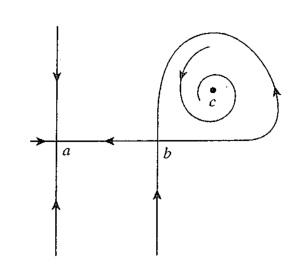
\includegraphics[width=0.4\textwidth]{attractor_portrait_2dsystem}
  (b)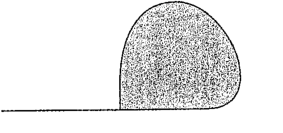
\includegraphics[width=0.5\textwidth]{attractor_2dsystem}
  \caption[The global attractor of a 2d system]{
    (a) \Statesp\ portrait of a 2d system.
    (b) The corresponding global attractor.
  }
  \label{fig:attractor_portrait}
\end{figure}

The $\omega$-limit sets of equilibria, \po s, and homoclinic
orbits are the objects
themselves, so they all belong to the global attractor,
as we would expect. Meanwhile, concerning the stable and unstable manifolds,
we have the following theorem.
\begin{theorem}
  The unstable manifolds and bounded stable manifolds
  of a compact invariant set are contained in the global attractor.
  \label{them:unstable}
\end{theorem}
We stress that the global attractor does not contain unbounded
stable/unstable manifolds. Unstable manifolds are intrinsically bounded
in dissipative systems,
so we omit the word ``bounded'' in front of it in theorem
\ref{them:unstable}. The explanation is simple.
Let $\ssp(t)$  be a point in the unstable manifold of an invariant set $X$, \ie,
$\ssp(t) \in W^{u}(X)$, then $\ssp(t)$ approaches $X$ for $t\to -\infty$ by
definition,
and $\ssp(t) \in B$ when $t\to\infty$ because the system is dissipative with
$B$ an absorbing set. Therefore, unstable manifold $W^u(X)$ is bounded.
However, not all stable manifolds are bounded. For example, one\dmn\
dissipative system $\dot{\ssp} = -\lambda \ssp$, $\lambda>0$
has a global attractor $\ssp=0$, but its stable manifold
extends to $\ssp\to\pm\infty$.
Such a distinction between stable and unstable
manifolds in dissipative systems is crucial for us to understand the finite
dimensionality of such systems.
In an infinite\dmn\ system described by a PDE, an unstable
invariant structure usually has only a few unstable modes and
the rest, infinite many, are all stable modes. Only a finite
subset of these stable modes participates in the dynamics.
As we shall show in this thesis,
the rest stable modes are
decoupled from other modes, decay exponentially, and do not belong to
the global attractor.

In the example shown in \reffig{fig:attractor_portrait}(a),
the 3 equilibria $\{a, b, c\}$, the
stable manifold of $c$, the homoclinic orbit of $b$ and the
heteroclinic orbit from $b$ to $a$ compose the global attractor,
which is shown in \reffig{fig:attractor_portrait}(b).


\paragraph{The global attractor in the Lorenz system}
We now prove the existence of a global attractor for the Lorenz system
to illustrate the concepts introduced in this section.
Theorem \ref{them:attractor} tells us that the key point of showing the
existence of a global attractor is to find a compact absorbing set $B$
in the system. For Lorenz system
\begin{align*}
  \dot{x} & = -\sigma x + \sigma y \\
  \dot{y} & = rx - y - xz \\
  \dot{z} & = xy - bz
\end{align*}
with $\sigma, r, b > 0$, consider
\[
  V(x, y, z) = x^2 + y^2 + (z-r-\sigma)^2
  \,.
\]
Then,
\begin{align*}
  \frac{dV}{dt}
  & = -2\sigma x^2 - 2y^2 - 2bz^2 + 2b(r+\sigma)z \\
  & = -2\sigma x^2 - 2y^2 - b(z-r-\sigma)^2 -bz^2 + b(r+\sigma)^2 \\
  & \le -\alpha V + b(r+\sigma)^2
\end{align*}
Here $\alpha = \min(2\sigma, 2, b)$.
By the Gronwall inequality, we obtain
\[
  V \le \frac{2b(r+\sigma)^2}{\alpha}
  \,.
\]
\begin{lemma}
  (Gronwall's Inequality) If
  \[
    \frac{du}{dt} \le au+b
    \,,
  \]
  then
  \[
    \ssp(t) \le (\ssp_0 + \frac{b}{a})e^{at} - \frac{b}{a}
    \,.
  \]
  \label{lem:Gronwall}
\end{lemma}
Therefore, there is an absorbing sphere
$S$ with radius $(2b/\alpha)^{1/2}(r+\sigma)$ in Lorenz system.
So a global attractor exists and it is given as $\omega(S)$.

\subsection{The dimension of an attractor}

Though the \statesp\ $\pS$ may be infinite\dmn,
after a transient period of evolution,
the dynamics is usually
determined only by a finite number of degrees of freedom.
The global attractor lives in a finite\dmn\ subspace of the
\statesp. Consequently, the study of the dimension of the global
attractor is crucial for us to understand the longtime behavior of
this system.
According to \refref{FaOttYo83}, the types of dimensions of chaotic attractors
can be classified into three categories. One is \emph{fractal dimensions},
based purely on the
geometry of the attractor such as the
box-counting dimension $D_{C}$ and the Hausdorff dimension $D_H$.
The second type
incorporates the frequency with which a typical
trajectory visits various parts of the attractor, namely the natural
measure of the attractor, such as  the information dimension $D_I$,
correlation
dimension $D_\mu$\rf{GraPro83a}, and so on. The third one,
Kaplan-Yorke
dimension $D_{KY}$ is defined in terms of the dynamical properties of an
attractor rather than the geometry or the natural measure.
Kaplan and Yorke\rf{KapYor79a, FKYY83}
initially conjectured that $D_{KY} = D_{C}$, but later
it was shown that $D_{KY}$ is an upper bound of the information dimension.
Some comparison of these various definitions of dimension can be found in
\refrefs{FaOttYo83, GraPro83a,Hunt96}. In this subsection, we list some
representative definitions related to our research.

\paragraph{Box-counting dimension (capacity dimension, Kolmogorov dimension)}
By using a minimal set of balls with radius $\epsilon$ to cover the
attractor and record the number of balls $N(\epsilon)$,
the \emph{box-counting dimension}
is given by
\begin{equation}
  \label{eq:dc}
  D_C = \limsup_{\epsilon \to 0} \frac{\log N(\epsilon)}{\log(1/\epsilon)}
\end{equation}
Note, we can also use cubes of side length $\epsilon$, which
does not change the result.
Basically, $D_C$ tells us how dense the state points are inside the
attractor. Trivial cases, like $D_C = 1$ for a straight line and
$D_C = 2$ for an area, are within our expectation, but for
fractal objects, it usually produces fraction/irrational numbers.
For instance, $D_C = \log 3/ \log 2$ for the Sierpinski triangle shown in
\reffig{fig:sier-tri}.
\begin{figure}[h]
  \centering
  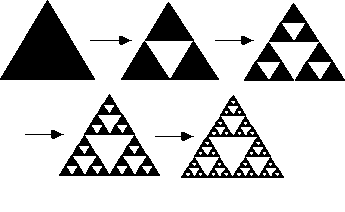
\includegraphics[width=0.5\textwidth]{sierp-det}
  \caption[The Sierpinski triangle]{
    The iterative process to get the Sierpinski triangle
    (from \refref{Devaney95}).
  }
  \label{fig:sier-tri}
\end{figure}


\paragraph{Hausdorff dimension}
The box-counting dimension uses balls of the same radius $\epsilon$
to cover the
attractor. Here, we try to cover the attractor with nonuniform open balls
whose radius is no larger than $\epsilon$.
First, we define the  $d$\dmn\ Hausdorff measure of a set $X$ in
$\pS$.
\begin{equation}
  \label{eq:haus_measure}
  \mathcal{H}^d(X) = \liminf_{\epsilon\to 0} \left\{\sum_{i=0}^\infty r_i^d :
    r_i < \epsilon \text{ and }
    X \subset \bigcup_{i=0}^\infty B_{r_i}(\ssp_i)
  \right\}
  \,.
\end{equation}
Here, $B_{r_i}(\ssp_i)$ is a $d$\dmn\
open ball centered at $\ssp_i$ with radius $r_i$. The definition
is analogous to the definition of Lebesgue measure. The basic idea is to estimate the
volume of the attractor by the total volume of finer and finer countable
$d$\dmn\ covering balls, where $d$ is a parameter in this measure. If $d$ is
larger than the actual dimension of the attractor, then $\mathcal{H}^d(X) = 0$.
For example, we need $1/2r$ circles whose radius is $r$
to cover a unit one\dmn\ segment. The total
area of these circles goes to zero when $r\to 0$. On the other hand, if $d$ is smaller
than the actual dimension, then $\mathcal{H}^d(X) \to \infty$. For instance, we need
infinitely long one\dmn\ segments to cover a two\dmn\ plane.
Based on this observation,
the \emph{Hausdorff dimension} of a compact set $X$ is defined as
\begin{equation}
  \label{eq:haus}
  D_H(X) = \inf \left\{d : \mathcal{H}^d(X) = 0 \text{ with } d > 0 \right\}
  \,.
\end{equation}
In general, the
Hausdorff dimension is not easy to get for a dynamical system.
But we do have an upper bound
\begin{equation}
  \label{eq:dhlsdc}
  D_H(X) \le D_C(X) \,.
\end{equation}
This relation is easy to understand. In defining Hausdorff dimension we have more
choices of the covering balls than that in box-counting dimension. Also,
\refeq{eq:haus_measure} is taking an infimum of all choices while $D_C$ takes the
supremum. For a rigorous proof of \refeq{eq:dhlsdc}, see \refref{Robinson2001}.

\paragraph{Information dimension}
The fractal dimension does not count the frequency with which each small region
is visited on the attractor. In order to incorporate such information,
the number of covering balls $N(\epsilon)$ is replaced by the entropy
function $-\sum^{N(\epsilon)} P_i \log P_i$, where $P_{i}$ is the probability
contained in cube $c_i$, namely the natural measure $\mu(c_i)$
of the attractor. The information dimension is then given as\rf{FaOttYo83}
\begin{equation}
  \label{eq:di}
  D_I = \lim_{\epsilon \to 0} \frac{-\displaystyle \sum^{N(\epsilon)}_{i=1}
    P_{i} \log P_i}{\log(1/\epsilon)}
  \,.
\end{equation}
The information dimension is no larger than the box-counting dimension, and
$D_I = D_C$ when the natural measure is constant across the attractor.

\paragraph{Kaplan-Yorke dimension (Lyapunov dimension)}
Kaplan and Yorke first proposed the idea of defining the dimension of a
chaotic attractor by the Lyapunov exponents
    \footnote{Actually, they used the magnitudes of
    multipliers or the `Lyapunov numbers', defined as the exponentials of
    the Lyapunov exponents. }
in \refref{KapYor79a}, and later they elaborated their proposal it in \refref{FKYY83}.
Here I sketch their basic idea\rf{RusHanOtt1980}.

Let $\lambda_1 \ge \cdots \ge \lambda_n$
are the Lyapunov spectrum
of an $n$\dmn\ chaotic system ($\lambda_1 > 0$). We try to
determine how many cubes needed to cover the neighborhood of a template
point $\ssp(0)$ as the system evolves. Suppose the neighborhood is an
$n$\dmn\ parallelogram with initially each edge oriented in the covariant
direction at $\ssp(0)$, and the number of $\epsilon$-cubes needed
to cover this parallelogram is $N(\epsilon)$; then after an infinitesimal
time $\delta t$, the neighborhood moves to $\ssp(\delta t)$ and the parallelogram
gets stretched/contracted in each covariant direction.
Choose some $j+1$ such that
$\lambda_{j+1} < 0$, we use a smaller cube with length
$e^{\lambda_{j+1} \delta t}\epsilon$ to cover the new neighborhood, then
\begin{equation}
N(e^{\lambda_{j+1} \delta t}\epsilon) =
\left( \prod_{i=1}^{j} e^{(\lambda_i - \lambda_{j+1})\delta t}\right)
N(\epsilon)
\label{eq:ky_relation}
\end{equation}
Let's explain the coefficient above. The $i$th direction with $i<j+1$
has been stretched by a factor $e^{\lambda_i \delta t}$, and the
new cube length is $e^{\lambda_{j+1} \delta t}\epsilon$, so it needs
$e^{(\lambda_i - \lambda_{j+1})\delta t}$ times more cubes along this direction.
Also, since choose $\lambda_{j+1} < 0$, then for the $i$th direction
with $i > j+1$, the original number of cubes along this direction
is enough to cover it, which means the above formula is actually
over-counting in this direction. The exponential law
$N(\epsilon) \propto \epsilon^{-d}$ from \refeq{eq:dc} is valid
when $\epsilon$ is small enough. Then \eqref{eq:ky_relation} reduces to
$(e^{\lambda_{j+1} \delta t}\epsilon)^{-d}  =
\prod_{i=1}^{j} e^{(\lambda_i - \lambda_{j+1})\delta t} \epsilon^{-d}$ and thus
\begin{equation}
  d(j) = j - \frac{\sum_{i=1}^{j} \lambda_i}{\lambda_{j+1}}
  \,.
  \label{eq:ky1}
\end{equation}
Just as stated above, formula \refeq{eq:ky1} is an upper bound of the dimension.
We need to find the smallest $d(j)$ under condition $\lambda_{j+1} < 0$.
\begin{align*}
  d(j+1) - d(j) &= 1 -\frac{\sum_{i=1}^{j+1} \lambda_i}{\lambda_{j+2}}
  + \frac{\sum_{i=1}^{j} \lambda_i}{\lambda_{j+1}} \\
  & = \frac{(\lambda_{j+2} - \lambda_{j+1})(\lambda_1 + \cdots + \lambda_{j+1})}
  {\lambda_{j+2}\lambda_{j+1}}
\end{align*}
Let $\lambda_1 + \cdots + \lambda_k \ge 0$ and
$\lambda_1 + \cdots + \lambda_{k+1} < 0$, then $d_{k+1} > d_{k}$ and
$d_k < d_{k-1}$. Therefore
\begin{equation}
  D_{KY} = k + \frac{\sum_{i=1}^{k} \lambda_i}{|\lambda_{k+1}|}
  \label{eq:ky2}
\end{equation}
with $k$ the largest number making $\lambda_1 + \cdots + \lambda_k$
non-negative.


\paragraph{Summary}
The definitions of dimension introduced in this section provide valuable
information about the size of the global attractor. However,
except for the Kaplan-Yorke dimension, all the other definitions
try to cover the global attractor with cubes statically. The information
about the topological structure of a global attractor has not been
used. On the other hand, strange attractors are almost always
fractal, and thus the dimension is an irrational number.
With this number, we
still do not know how many degrees of freedom are
needed to effectively describe the dynamics of a dissipative PDE in an
infinite\dmn\ space. In the next section, we introduce the concept of the
\emph{inertial manifold} that contains the global attractor and determines
the dynamics by a finite number of degrees of freedom.


\subsection{Inertial manifold}
\label{subsec:IM}

For dissipative chaotic systems, asymptotic orbits are contained in a
lower\dmn\ subspace of
the \statesp\ $\pS$. Thus the effective dynamics can be described by a
finite number of degrees of freedom.
A global attractor usually has fractal dimension, which make it hard to
analyze, so we need to construct
a `tight' smooth manifold that encloses it, and whose dimension gives the
effective degrees of freedom of this system. This
is called the \emph{inertial manifold}\rf{Foias1988a,
Robinson1995, infdymnon, Robinson2001}.

Here we use the concept of
``\emph{slaving}'' in order to understand how the transition from infinite\dmn\
space to finite\dmn\ subspace happens. Let $\ssp(t)$ be a dynamical
system in an infinite\dmn\ \statesp\ $\pS$ governed by
\begin{equation}
  \label{eq:proto}
  \frac{d\ssp}{dt} + \vlo \ssp + \vno(\ssp) = 0
  \,.
\end{equation}
We split the ``velocity'' field into a linear part and a nonlinear part.
Linear
operator $\vlo$ is usually a negative Laplace operator or a higher-order spatial
derivative. If the nonlinear term $\vno(\ssp)$ is weak, then the dynamics is
largely determined by the eigenspaces of $\vlo$. That is why in practice
solution $\ssp(t)$ is usually expanded in terms of the eigenvectors of $\vlo$.
Specifically, if $\vlo$ is a negative Laplace operator, and the system is
defined either on an infinite or periodic domain,
then its eigenvectors are pure Fourier modes.
$\ssp(t)$ is determined by an infinite number of its
Fourier coefficients. We say that \highmode s are \emph{slaved to}
\lowmode s if
there is a map that uniquely maps \lowmode s to \highmode s. With such a map,
the dynamics of the system is totally determined by the \lowmode s. To make this
idea more precise,
let $P_n$ denote the projection from \statesp\ $\pS$ to the subspace spanned
by the eigenvectors of $\vlo$ corresponding to its smallest $n$ eigenvalues,
and let $Q_n = I - P_n$. Ranges of $P_n$ and $Q_n$ are denoted
as $P_n\pS$ and $Q_n\pS$ respectively.
Subspaces $P_n\pS$ and $Q_n\pS$ contain the low and \highmode s of
the solution $\ssp(t)$.
Though $Q_n\pS$ is infinite\dmn\, the effective dynamics is trapped in a
finite\dmn\ subspace of $\pS$. So we anticipate that there is
a map $\Phi:P_n\pS\mapsto Q_n\pS$ that determines the \highmode s
of $\ssp(t)$ given its \lowmode s.
Denote
\begin{equation}
  \label{eq:pq}
  p(t) = P_n\ssp(t) \,,\quad q(t) = Q_n\ssp(t)
\end{equation}
and project \eqref{eq:proto} onto $P_n\pS$, we obtain
\begin{equation}
  \label{eq:projected}
  \frac{dp}{dt} + \vlo p + P_n \vno(p+\Phi(p)) = 0
  \,.
\end{equation}
So we have reduced the dynamics to a
subspace given the existence of such a mapping $\Phi$.
Equation \eqref{eq:projected} is
called the \emph{inertial form} of this system.
The graph of $\Phi$
\[
  \mathcal{G}[\Phi] := \{\ssp: \ssp = p + \Phi(p)\,, p\in P_n\pS\}
\]
defines an $n$\dmn\ manifold $\IM$. This manifold is
proved\rf{Robinson2001} to be an inertial manifold
defined below.
\begin{definition}
  An inertial manifold $\IM$ is a finite\dmn\ Lipschitz manifold,
  which is positively invariant and attracts all trajectories exponentially,
  \begin{equation}
    \label{eq:im_def}
    \dist(\semiflow{t}\ssp_0, \IM) \le C(|\ssp_0|)e^{-kt}\quad
    \text{for some } k > 0 \text{ and all } \ssp_0 \in \pS
    \,.
  \end{equation}
\end{definition}
Lipschitz means $|\Phi(p_1) - \Phi(p_2)| \le L |p_1 - p_2|$ for any
$p_1, p_2\in P_n\pS$ and some positive
constant $L$. The Lipschitz condition
is required for the initial form \refeq{eq:projected} to
have unique solutions.
There are several differences between a global attractor and an inertial manifold.
First, an inertial manifold, by definition, has an integer number of dimensions, but
a global attractor of a chaotic system usually has a fractal dimension.
Second, an inertial manifold is
only positive-invariant \refeq{eq:pos_invar}, but a global attractor is the maximal
invariant subset of $\pS$. Therefore, the global attractor is contained in the
inertial manifold. Third, a global attractor can attract trajectories arbitrarily slowly
by definition \refeq{eq:ga2}, while an inertial manifold attracts trajectories
exponentially fast.

Equation \refeq{eq:im_def} also implies that the error introduced by
approximating $q(t)$ by $\Phi(p(t)$ decays exponentially with time:
\begin{equation}
  |q(t)-\Phi(p(t))| \le C(|\ssp_0|)e^{-kt}
  \,.
  \label{eq:im_def2}
\end{equation}
The reason is as follows. From the definition of distance of two sets
\refeq{eq:dist} and the fact that
$\ssp(t) = \semiflow{t}\ssp_0 = P_n\ssp + Q_n\ssp$, we have
\[
  \dist(\semiflow{t}\ssp_0, \IM) = \inf_{s\in P_n\pS} \left|(P_n\ssp + Q_n\ssp) -
    (s + \Phi(s))\right|
  \,.
\]
Since projection $P_n$ and $Q_n$ are orthogonal to each other, the above
infimum is reached when $s = P_nu$. Thus we have we
\[
  \dist(\semiflow{t}\ssp_0, \IM) = \left|Q_n\ssp - \Phi(P_n\ssp)) \right| =
  \left|q(t) - \Phi(p(t)) \right|
  \,.
\]
The equivalence between \refeq{eq:im_def} and \refeq{eq:im_def2} confirms that
the idea of \emph{mode slaving} works in a dissipative system given the existence
of an inertial manifold. For any point in the \statesp, we can find an
approximate state on the inertial manifold. These two states share the same \lowmode s
and only differ in their
\highmode s. \Highmode s are slaved to \lowmode s,
and their difference decays exponentially. So after a short transient
period, all orbits are effectively captured by the inertial manifold.

An inertial manifold exists in systems which possess the
\emph{strong squeezing property}\rf{Robinson2001}. A system says to have the
strong squeezing property if for any two solutions
$\ssp(t) = p(t) + q(t)$ and $\bar{\ssp}(t) =  \bar{p}(t) + \bar{q}(t)$, the following
two properties hold. (i) the \emph{cone invariance property}: if
\begin{equation}
  \label{eq:ssp1}
  |q(0) - \bar{q}(0)| \le |p(0) - \bar{p}(0)|
\end{equation}
then
\begin{equation}
  \label{eq:ssp2}
  |q(t) - \bar{q}(t)| \le |p(t) - \bar{p}(t)|
\end{equation}
for all $t \le 0$, and (ii) the \emph{decay property}: if
\begin{equation}
  \label{eq:ssp3}
  |q(t) - \bar{q}(t)| \ge |p(t) - \bar{p}(t)|
\end{equation}
then
\begin{equation}
  \label{eq:ssp4}
  |q(t) - \bar{q}(t)| \le |q(0) - \bar{q}(0)| e^{-kt}
\end{equation}
for some $k > 0$. The first property says that initially if two states
satisfy the Lipschitz condition with Lipschitz constant $1$, then
such a Lipschitz condition holds at any later time.
The second property accounts for the exponential attraction \refeq{eq:im_def}
of the inertial manifold.
In practice, it is hard to verify the strong squeezing property
directly. Here we provide an intuitive argument to
show that a large gap in the eigenspectrum of operator $\vlo$ in \refeq{eq:proto}
leads to the strong squeezing property. Let $\vlo$ have eigenvalues
$\lambda_1 \le \lambda_2 \le \cdots$. Inertial form
\refeq{eq:projected} describes the dynamics of the $n$ \lowmode s
which correspond to eigenvalues $\lambda_1,\cdots, \lambda_n$.
The minimal growth rate in subspace $P_n\pS$ is $-\lambda_n$. While, the rest
\highmode s should have approximately the largest growing rate $-\lambda_{n+1}$. If
$-\lambda_{n+1}$ is far smaller than $-\lambda_n$, then we anticipate that
$|p(t)-\bar{p}(t)|$ should grow faster than $|q(t)-\bar{q}(t)|$, so
\refeq{eq:ssp2} holds.
Also, if $-\lambda_{n+1} < 0$, then
\refeq{eq:ssp4} should hold too. Note that we have not taken into consideration the
coupling between low and \highmode s by the nonlinear term
$\vno(\ssp)$ in \refeq{eq:proto}.
Therefore, to ensure strong squeezing property,
the threshold of gap $\lambda_{n+1}-\lambda_{n}$
should depend on $\vno(\ssp)$. Such a \emph{spectral gap condition}
is precisely described in the following theorem.
\begin{theorem}
  \label{them:spectGap}
  If $\vno(\ssp)$ is Lipschitz
  \[
    |\vno(\ssp) - \vno(v)| \le C_1 |\ssp - v|, \quad \ssp, v \in \pS
  \]
  and eigenvalues of $\vlo$ in \refeq{eq:proto} satisfies
  \begin{equation}
    \label{eq:im_gap}
    \lambda_{n+1} - \lambda_n > 4 C_1
  \end{equation}
  for some integer $n$, then the strong squeezing property holds, with
  $k$ in \refeq{eq:ssp4} satisfying $k \ge \lambda_n + 2C_1$.
\end{theorem}
See\rf{Robinson2001} for the proof of this theorem.

The existence of an inertial manifold has been proved
for many chaotic or turbulent systems such as \KSe, \cGLe\ and
the two\dmn\ \NSe\rf{infdymnon}.
Also, numerical methods such as Euler-Galerkin\rf{foias88} and nonlinear
Galerkin method\rf{Marion1989} have been proposed to approximate
inertial manifolds. Approximating
mapping $\Phi:P_n\pS\mapsto Q_n\pS$ requires choosing an appropriate $n$ first.
If $n$ is smaller than the dimension of the inertial manifold, then $\Phi$
fails to describe the inertial manifold. However, if $n$
is far larger than the dimension of the inertial manifold, then simulations on
such approximations to the inertial manifold
are not numerically efficient.
At present, one uses empirical or some test number to truncate the
original system. For example, in\rf{foias88}, 3 modes are
used to represent the inertial manifold of the one\dmn\ \KSe, but this
truncated model is not sufficient to preserve the bifurcation diagram.
At the same time, mathematical upper bounds for the dimension are not always tight.
Therefore, little is known about the exact dimension of inertial manifolds in
dissipative chaotic systems.

%%% ======================================================================
\section{\CLvs}
\label{sec:covVecs}

The recent progress
in numerical methods to calculate \emph{\cLv}s\rf{GiChLiPo12, KuPa12}
has motivated us to explore an inertial manifold by
\cLvs\ locally through a statistical study of the tangency among
\cLvs\rf{YaTaGiChRa08} and
difference vector projection\rf{YaRa11}. The number of the \cLvs\ needed
for locally spanning the inertial manifold is
regarded as the dimension of an inertial manifold. The key observation
in this study is that tangent space can be decomposed into an
entangled ``physical'' subspace and its complement, a contracting
disentangled subspace.
The latter plays no role in the longtime behavior
on the inertial manifold.

In this section, we will introduce covariant vectors (often called
``covariant Lyapunov vectors'' in the literature\rf{GiChLiPo12,
ginelli-2007-99}) associated with \po s and ergodic orbits. The
general setup is that we have an autonomous continuous flow described by
\begin{equation}
  \label{eq:flow}
  \dot{\ssp} = \vel(\ssp) \,, \quad \ssp(x, t) \in \reals^n
  \,.
\end{equation}
The corresponding time-forward trajectory starting from $\ssp_0$ is
$\ssp(t)=\flow{t}{\ssp_0}$.
In the linear approximation, the equation that governs
the deformation of an infinitesimal neighborhood of
$\ssp(t)$ (dynamics in tangent space) is
\begin{equation}
  \label{eq:stab}
  \frac{d}{dt}\delta \ssp = A \delta\ssp \,, \quad
  A = \frac{\partial \vel}{\partial \ssp}
  \,.
\end{equation}
Matrix $A$ is called the stability matrix of the flow. It describes the
rates of instantaneous expansion/contraction and shearing in the tangent space.
The \JacobianM\ of the flow transports linear perturbation along the orbit:
\begin{equation}
  \label{eq:jacob}
  \delta \ssp(\ssp, t)=\jMps^\zeit(\ssp_0, 0)\,\delta \ssp(\ssp_0, 0)
\end{equation}
Here we make it explicit that the infinitesimal deformation
$\delta \ssp$ depends on both
the orbit and time. The \JacobianM\ is obtained by integrating equation
\begin{equation}
  \label{eq:tangentDynamics}
  \frac{d}{dt}\jMps = A \jMps \,, \quad
  J_0 = I
  \,.
\end{equation}
\JacobianM\ satisfies the semi-group multiplicative property (chain rule)
along an orbit,
\begin{equation}
  \jMps^{\zeit-\zeit_{0}}(\ssp(\zeit_{0}) ,\zeit_{0})
  =
  \jMps^{\zeit-\zeit_{1}}(\ssp(\zeit_{1}),\zeit_{1})
  \jMps^{\zeit_{1}-\zeit_{0}}(\ssp(\zeit_{0}),\zeit_{0})
  \,.
  \label{eq:xjacobian}
\end{equation}


\subsection{\Fv s}
\label{sect:LinStab}

For a point
$\ssp(\zeit)$ on a \po\ $p$ of period \period{p},
\begin{equation}
  \label{eq:fm}
  \jMps_p=\jMps^{\period{p}}(\ssp, \zeit)
\end{equation}
is called the Floquet matrix
(monodromy matrix), and its
eigenvalues the Floquet multipliers $\ExpaEig_{j}$.
The $j$th Floquet multiplier is a dimensionless ratio of
the final/initial
deformation along the $j$th eigendirection. It is an intrinsic, local
property of a smooth flow, invariant under all smooth coordinate
transformations. The associated
\Fv s $\jEigvec[j](\ssp)$,
\begin{equation}
  \label{eq:fv}
  \jMps_p\,\jEigvec[j]=\ExpaEig_{j}\jEigvec[j]
\end{equation} define the invariant
directions of the tangent space at periodic point
$\ssp(\zeit)\in p$. Evolving a small initial perturbation aligned with
an expanding Floquet direction will generate the corresponding
unstable manifold along
the \po. Written in exponential form
\[
  \ExpaEig_{j} = \exp(\period{p}\Lyap^{(j)}_p)\
  = \exp(\period{p}\eigRe[j] + i\theta_j)
  \,,
\]
where $\Lyap^{(j)}_p$\footnote{Here, subscript $p$ emphasizes
  that it is
  associated with a \po\ so as to distinguish it
  with the Lyapunov exponents defined in
  the next section.} are the
Floquet exponents.
Floquet multipliers are either real,
$\theta_j = 0, \pi$, or form
complex pairs, $\{\ExpaEig_{j},\ExpaEig_{j+1}\} =
\{|\ExpaEig_{j}|\exp(i\theta_j),|\ExpaEig_{j}|\exp(-i\theta_j)\}$, $0
<\theta_j <\pi$. The real parts of the
Floquet exponents
\begin{equation}
  \label{eq:fe}
  \eigRe[j] = (\ln|\ExpaEig_{j}|)/\period{p}
\end{equation}
describe the mean contraction or
expansion rates per one period of the orbit.
Appendix \ref{sec:floq} talks about the form of the \JacobianM\ of
a general linear flow with periodic coefficients.

\subsection{\CLv s}

For a \po, the Jacobian matrix of $n$ periods is the $n$th power of the Jacobian
corresponding to a single period. However, for an ergodic orbit, there is no
such simple relation. Integrating \JacobianM\ by
\refeq{eq:tangentDynamics} cannot be avoided for studying asymptotic stability of this
orbit. However, similar to \Fv s of a \po, a set of \cLvs\
exists for an ergodic orbit.
\emph{Multiplicative ergodic theorem}\rf{lyaos,ruelle79} says that the forward and backward
Oseledets matrices
\begin{equation}
  \Xi^{\pm}(\ssp) :=\lim_{t\to\pm\infty}[J^t(\ssp)^\top J^{t}(\ssp)]^{1/2t}
  \label{eq:oseledets}
\end{equation}
both exist for an invertible dynamical system equipped with an invariant measure.
Their eigenvalues are
$e^{\Lyap^{+}_1(\ssp)}<\cdots<e^{\Lyap^{+}_s(\ssp)}$,
and $e^{\Lyap^{-}_1(\ssp)}>\cdots>e^{\Lyap^{-}_s(\ssp)}$ respectively,
with $\Lyap^{\pm}_i(\ssp)$ the
Lyapunov exponents (characteristic exponents) and $s$
the total number of distinct exponents ($s\le n$). For an ergodic system,
Lyapunov exponents are the same almost everywhere, and
\begin{equation}
  \label{eq:lyap}
  \Lyap^{+}_i(\ssp)=-\Lyap^{-}_{i}(\ssp)=\Lyap_i
\end{equation}
The corresponding eigenspaces
$U^\pm_1(\ssp), \cdots, U^\pm_s(\ssp)$
can be used to construct the forward and backward invariant subspaces:
\begin{align*}
  V^+_i(\ssp) & = U^+_1(\ssp) \oplus \cdots \oplus U^+_i(\ssp) \\
  V^-_i(\ssp) & = U^-_i(\ssp) \oplus \cdots \oplus U^-_{s}(\ssp)
  \,.
\end{align*}
So the intersections
\begin{equation}
  \label{eq:inter}
  W_i(\ssp)=V^+_i(\ssp)\cap V^-_i(\ssp)
\end{equation}
are dynamically
forward and backward invariant: $J^{\pm t}(\ssp)W_i(\ssp) \to W_i(\flow{\pm t}{\ssp})$,
$i = 1, 2,\cdots,s$. \refeq{eq:inter} is called the Oseledets splitting.
The expansion rate in the invariant subspace $W_i(\ssp)$ is given
by the corresponding Lyapunov exponent,
\begin{equation}
  \label{eq:lyapunov}
  \lim_{t\to\pm\infty}\frac{1}{|t|}\ln\norm{J^t(\ssp)v}
  =\lim_{t\to\pm\infty}\frac{1}{|t|}\ln\norm{[J^t(\ssp)^\top J^t(\ssp)]^{1/2}v}
  = \pm\Lyap_i
  \,,\quad v\in W_i(\ssp)
  \,.
\end{equation}
If a Lyapunov exponent is nondegenerate, the corresponding
subspace $W_i(\ssp)$ reduces to a vector, called \emph{\cLv}.
For \po s, these $\Lyap_i$
(evaluated numerically as $\zeit\to\infty$ limits of many repeats of the
prime period $\period{}$) coincide with the real parts of Floquet exponents
\refeq{eq:fe}. Subspace $W_i(\ssp)$ coincides with
a \Fv, or, if there is degeneracy, a subspace
spanned by \Fv s.

The reorthonormalization procedure
formulated by Benettin \etal\rf{bene80a}
is
the standard way to calculate the full spectrum of Lyapunov exponents,
and it is shown\rf{ErshPot98}
that the orthogonal vectors produced at the end of
this procedure converge to $U_i^{-}(\ssp)$, eigenvectors of $\Xi^{-}(\ssp)$, called
the Gram-Schmidt (GS) vectors (or backward Lyapunov vectors).
Based on this technique,
Wolf \etal\rf{WoSa07} and
Ginelli \etal\rf{GiChLiPo12, ginelli-2007-99}
independently invented distinct methods to recover \cLv s
from GS vectors. Here, we should emphasize that GS vectors are
not invariant. Except for the leading one, all of them depend on
the specific inner product imposed by the dynamics. Also, the local expansion
rates of \cLv s are not
identical to the local expansion rates of GS vectors. Specifically for
\po s, \Fv s depend on no norm and map forward and
backward as $\jEigvec[j] \to \jMps\,\jEigvec[j]$ under time evolution.
In contrast, the linearized dynamics does not transport GS vectors into
the tangent space computed further downstream. For a detailed
comparison, please see\rf{KuPa12, YaRa10}.

\subsection{\CLv s algorithm}
\label{subsec:clvs}

\begin{figure}
  \centering
  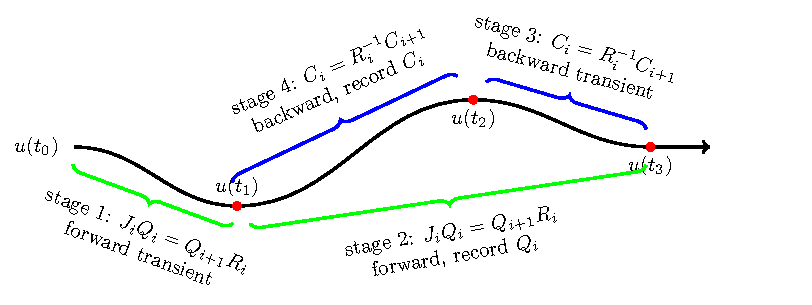
\includegraphics[width=1\textwidth]{cLv}
  \caption[Four stages of \cLv\ algorithm]
  {Four stages of \cLv\ algorithm.
    The black line is a part of
    a long ergodic trajectory.}
  \label{fig:CLV}
\end{figure}
Here we briefly introduce the method used by
Ginelli \etal\rf{GiChLiPo12, ginelli-2007-99}
to extract
\cLvs\ from GS vectors. The setup is the same as computing Lyapunov
exponents. We follow a long ergodic trajectory and integrate
the linearized dynamics in tangent space \eqref{eq:tangentDynamics}
with orthonormalization regularly, shown as the first two stages in
\reffig{fig:CLV}.
Here, $J_i$ is the short-time \JacobianM,
and $Q_{i+1}R_i$ is the $QR$ decomposition of $J_iQ_i$.
We use the new generated orthonormal matrix $Q_{i+1}$ as the initial condition
for the next short-time integration of \eqref{eq:tangentDynamics}.
Therefore, if we choose an appropriate time length of each integration segment,
we can effectively avoid numerical instability by repeated $QR$ decomposition.
Set the initial
deformation matrix $Q_0 = I$, then after $n$ steps in stage 1, we obtain
\[
  J_{n-1}\cdots J_0 = Q_n R_n\cdots R_0
  \,.
\]
The diagonal elements
of upper-triangular
matrices $R_i$ store local
Lyapunov exponents, longtime average of which gives the Lyapunov
exponents of this system. In stage 1, we discard all these
upper-triangular matrices $R_i$. We assume that $Q_i$ converges
to the GS vectors after stage 1, and start to record $R_i$ in
stage 2. Since the first $m$ GS vectors span the same subspace as the
first $m$ \cLv s, which means
\begin{equation}
  \label{eq:cv_T}
  T_i = Q_iC_i
  \,.
\end{equation}
Here $T_i = [W_1, W_2,\cdots, W_n]$ refers to the matrix whose columns
are \cLv s at step $i$ of this algorithm.
$C_i$ is an upper-triangular matrix, giving the expansion
coefficients of \cLv s in the GS basis. Since $J_{i-1}Q_{i-1}=Q_iR_i$,
we have $T_i = J_{i-1} Q_{i-1} R^{-1}_{i}C_i$.
Also since $T_{i-1} = Q_{i-1}C_{i-1}$, we get
\begin{equation}
  \label{eq:cv_T2}
  T_{i} = J_{i-1}T_{i-1}C_{i-1}^{-1}R^{-1}_{i}C_i
\end{equation}
Since $T_i$ is invariant in the
tangent space, namely, $J_{i-1}T_{i-1}=T_iD_i$ with
$D_i$ a diagonal matrix concerning the stretching and
contraction of \cLv s. Substitute it into \refeq{eq:cv_T2}, we get
$I = D_iC_{i-1}^{-1}R^{-1}_{i}C_i$. Therefore,
we obtain the backward dynamics of
matrix $C_i$ :
\begin{equation}
  \label{eq:cv_back}
  C_{i-1} = R^{-1}_{i} C_iD_i
\end{equation}
Numerically, $D_i$ is
not formed explicitly since it is only a normalization factor.
Ginelli \etal\rf{GiChLiPo12, ginelli-2007-99}  cleverly uncover
this backward dynamics and show that $C_i$ converges after a sufficient
number of iterations (stage 3 in \reffig{fig:CLV}). We choose an arbitrary
upper-triangular matrix as the initial input for the backward iteration
\refeq{eq:cv_back}, $R_i$ are those upper-triangular matrices recorded during
stage 2, and $R_i^{-1}$ are also upper-triangular. The product of two
upper-triangular matrices is still upper-triangular. Thus, backward iteration
\refeq{eq:cv_back} guarantees that $C_i$ are all upper-triangular.
This process
is continued in stage 4 in \reffig{fig:CLV}, and $C_i$ are recorded
at this stage.
For trajectory segment $\ssp(t_1)$ to $\ssp(t_2)$ in \reffig{fig:CLV},
we have the converged GS basis $Q_i$ and the converged $C_i$,
then by \refeq{eq:cv_T},
we obtain the \cLv s corresponding to this segment.

\CLv\ algorithm is invented to stratify the tangent spaces along
an ergodic trajectory, so it is hard to observe
degeneracy numerically. However, for \po s, it is
possible that some \Fv s form conjugate complex pairs.
When this algorithm is applied to \po s, it is reduced
to a combination of simultaneous iteration and inverse
power iteration;
consequently, complex conjugate pairs cannot be told apart.
This
means that we need to pay attention to the two\dmn\ rotation
when checking the convergence of each stage in \reffig{fig:CLV}.
As is shown in \refchap{chap:ped}, a complex conjugate pair
of \Fv s can be extracted from a converged
two\dmn\ subspace.

%======================================================================
\subsection{\Psd\ algorithm}
\label{subsec:psd}

\begin{figure}
  \centering
  \begin{align*}
    \small
    \setlength\arraycolsep{1pt}
    \renewcommand{\arraystretch}{0.7}
    \begin{bmatrix}
      x & x & x & x & x & x \\
      x & x & x & x & x & x \\
      x & x & x & x & x & x \\
      x & x & x & x & x & x \\
      x & x & x & x & x & x \\
      x & x & x & x & x & x \\
    \end{bmatrix}
    \begin{bmatrix}
      x & x & x & x & x & x \\
      x & x & x & x & x & x \\
      x & x & x & x & x & x \\
      x & x & x & x & x & x \\
      x & x & x & x & x & x \\
      x & x & x & x & x & x \\
    \end{bmatrix}
    \begin{bmatrix}
      x & x & x & x & x & x \\
      x & x & x & x & x & x \\
      x & x & x & x & x & x \\
      x & x & x & x & x & x \\
      x & x & x & x & x & x \\
      x & x & x & x & x & x \\
    \end{bmatrix}
        & \xrightarrow{\normalsize \text{stage 1}}
        % & \overset{\text{\normalsize stage 1}}{\large \to}
            \small
            \setlength\arraycolsep{1pt}
            \renewcommand{\arraystretch}{0.7}
            \begin{bmatrix}
              x & x & x & x & x & x \\
              x & x & x & x & x & x \\
              & x & x & x & x & x \\
              &   & x & x & x & x \\
              &   &   & x & x & x \\
              &   &   &   & x & x \\
            \end{bmatrix}
    \begin{bmatrix}
      x & x & x & x & x & x \\
      & x & x & x & x & x \\
      &   & x & x & x & x \\
      &   &   & x & x & x \\
      &   &   &   & x & x \\
      &   &   &   &   & x \\
    \end{bmatrix}
    \begin{bmatrix}
      x & x & x & x & x & x \\
      & x & x & x & x & x \\
      &   & x & x & x & x \\
      &   &   & x & x & x \\
      &   &   &   & x & x \\
      &   &   &   &   & x \\
    \end{bmatrix} \\
        & \xrightarrow{\normalsize \text{stage 2}}
          \small
          \setlength\arraycolsep{1pt}
          \renewcommand{\arraystretch}{0.7}
          \begin{bmatrix}
            x & x & x & x & x & x \\
            & x & x & x & x & x \\
            & x & x & x & x & x \\
            &   &   & x & x & x \\
            &   &   &   & x & x \\
            &   &   &   &   & x \\
          \end{bmatrix}
    \begin{bmatrix}
      x & x & x & x & x & x \\
      & x & x & x & x & x \\
      &   & x & x & x & x \\
      &   &   & x & x & x \\
      &   &   &   & x & x \\
      &   &   &   &   & x \\
    \end{bmatrix}
    \begin{bmatrix}
      x & x & x & x & x & x \\
      & x & x & x & x & x \\
      &   & x & x & x & x \\
      &   &   & x & x & x \\
      &   &   &   & x & x \\
      &   &   &   &   & x \\
    \end{bmatrix}
  \end{align*}
  \caption[Two stages of \psd\ algorithm ]
  {Two stages of \psd\ algorithm illustrated by
    three $[6\!\times\! 6]$ matrices. Empty locations are zeros.}
  \label{fig:PSD}
\end{figure}
Here, we review another algorithm related to our work.
The double-implicit-shift QR algorithm\rf{Trefethen97,DSWatkins}
is the standard way
of solving the eigen-problem of a single matrix in many numerical packages,
such as the
\texttt{eig()} function in Matlab.
Bojanczyk \etal\rf{Bojanczyk92theperiodic}
extend this
idea to obtain \emph{\psd} of the product of a sequence of matrices. Later on,
Kurt Lust\rf{Lust01} describes the implementation details and provides
the corresponding
Fortran code.
On the other hand, by use of the chain rule \eqref{eq:xjacobian}, the
\JacobianM\ can be decomposed into a product of short-time
Jacobians with the same dimension. Therefore, \psd\ is well suited for computing
Floquet exponents.

As illustrated in \reffig{fig:PSD}, \psd\ proceeds in two stages.
First, the sequence
of matrices is transformed to the \emph{Hessenberg-Triangular} form,
one of which has upper-Hessenberg form while the others
are upper-triangular,
by a series of Householder transformations\rf{Trefethen97}.
The second stage tries to diminish the sub-diagonal components of
the Hessenberg matrix until it becomes quasi-upper-triangular,
that is, there are some
$[2\!\times\! 2]$ blocks on the diagonal corresponding to
complex eigenvalues. The eigenvalues of the matrix product are
given by the products of all individual matrices' diagonal elements.
However, \psd\ is not sufficient for extracting eigenvectors, except the leading one.
Kurt Lust\rf{Lust01} claims to formulate the corresponding
\Fv\ algorithm, but to
the best of our knowledge, such an algorithm is not present in the literature.
Fortunately, Granat \etal\rf{GranatK06} have proposed a method to reorder diagonal
elements
after \psd. This provides an elegant way to compute \Fv s as we will see in
\refchap{chap:ped}.

%\renewcommand{\inputfile}{\version\ - edited 2008-06-26 cycExp}
% \section{Cycle expansions}
% $Author: predrag $ $Date: 2008-06-26 10:30:57 -0400 (Thu, 26 Jun 2008) $
%  label{sec:cycExp}







% \beq
% 1/\zeta   =  \prod_p { ( 1- t_p)} = 1 - \sumprime_{\{p_1 p_2 \dots p_k\}}
%         (-1)^{k+1} t_{p_1} t_{p_2} \dots t_{p_k}
% \ee{pseudo0}


%%% ======================================================================
%
%\chapter{Symmetries in dynamical systems}
%\label{chap:Symmetry}
%
%% siminos/xiong/thesis/chapters/symIntro.tex
% $Author: predrag $ $Date: 2021-06-19 11:30:00 -0400 (Sat, 19 Jun 2021) $

Symmetries play an important role in physics. In the study of
pattern formation\rf{cross93},
patterns with different symmetries form under different boundary conditions or
initial conditions. By considering symmetries only, quite a few
prototype equations such as \cGLe\rf{AKcgl02}
are proposed and have abundant applications in many fields.
So, in general,
symmetries help create a wonderful physical world for us.
However, in the analysis of chaotic systems, symmetries introduce
drifts of orbits along the symmetry directions and thus make the geometrical
structure of the global attractor more complicated than it really is.
In this case,
symmetries should be reduced before we conducting any analysis. In this chapter,
we review the basic notions of group theory, symmetry reduction
methods, and establish the relation between dynamics in the full \statesp\
and that in the symmetry-reduced \statesp.
% Finally, we factorize the
% evolution operator with respect to symmetries of the system so as to
% simplify the cycle averaging formula.

%% siminos/xiong/thesis/chapters/symGroup.tex
% $Author: predrag $ $Date: 2021-06-19 11:30:00 -0400 (Sat, 19 Jun 2021) $

\section{Group theory and symmetries: a review}
\label{sect:group}

In quantum mechanics, whenever a system exhibits some symmetry, the
corresponding symmetry group commutes with the Hamiltonian of this
system, namely, $[U(\LieEl), H] = U(\LieEl)H - HU(\LieEl) = 0$. Here
$U(\LieEl)$ denotes the operation corresponding to symmetry $g$ whose
meaning will be explained soon. The set of eigenstates with degeneracy
$\ell$, $\{\phi_1, \phi_2, \cdots, \phi_\ell\}$, corresponding to the same
system energy $H\psi_i = E_n\psi_i$, is invariant under the symmetry
since $U(\LieEl)\psi_i$ are also eigenvectors for the same energy.
This information helps us understand the spectrum of a Hamiltonian and
the quantum mechanical selection rules. We now apply the same idea to
the classical {\evOper} $\Lop^t(\ssp_e, \ssp_s)$
for a system $\flow{t}{\ssp}$ equivariant under a discrete symmetry group
$\Group=\{e, \LieEl_2, \LieEl_3,\cdots, \LieEl_{|\Group|}\}$ of order
$|\Group|$:
\begin{equation}
  \label{eq:equiva}
  \flow{t}{{D}\LieEl}\ssp)={D}(\LieEl)\,\flow{t}{\ssp} \quad \text{for}
  \quad \forall
  \LieEl\in\Group
  \,.
\end{equation}
We start with a review of some basic facts of
the group representation theory. Some examples of good references
on this topic are \refref{Hamermesh62, Tinkham}.

Suppose group $\Group$ acts on a linear space $V$ and function
$\rho(\ssp)$ is defined on this space $\ssp\in V$. Each element
$\LieEl\in\Group$ will transform point $\ssp$ to ${D}(\LieEl)\ssp$. At
the same time, $\rho(\ssp)$ is transformed to $\rho'(\ssp)$. The value
$\rho(\ssp)$ is unchanged after state point $\ssp$ is transformed to
${D}(\LieEl)\ssp$, so $\rho'({D}(\LieEl)\ssp) = \rho(\ssp)$. Denote
$U(\LieEl)\rho(\ssp)=\rho'(\ssp)$, so we have
\begin{equation}
  \label{eq:ogfx}
  U(\LieEl)\rho(\ssp) = \rho({D}(\LieEl)^{-1}\ssp)
  \,.
\end{equation}
This is how functions are transformed by group operations. Note, $D(\LieEl)$
is the representation of $G$ in the form of space transformation matrices.
The
operator $U(\LieEl)$, which acts on the function space, is not the same as
group operation ${D}(\LieEl)$, so \refeq{eq:ogfx} does not mean that
$\rho(\ssp)$ is invariant under $\Group$. \refExam{exam:C3matrRep} gives
the space transformation matrices of $\Zn{3}$.

%%%%%%%%%%%%%%%%%%%%%%%%%%%%%%%%%%%%%%%%%%%%%%%%%%%%%%%%%%%%%%%%%%%%%%
\exampl{A matrix representation of cyclic group $\Zn{3}$.}{
  \label{exam:C3matrRep}                                    \inCB
  A 3\dmn\ matrix representation of the 3-element cyclic group
  $\Zn{3}=\{e,C^{1/3},C^{2/3}\}$ is given by the three rotations by
  $2\pi/3$ around the $z$-axis in a 3\dmn\ \statesp,
  \bea
  {D}(e) &=&
  \begin{bmatrix}
    1 & & \\
    & 1 & \\
    & & 1
  \end{bmatrix}
  \,,\quad
  {D}(C^{1/3}) =
  \begin{bmatrix}
    \cos\frac{2\pi}{3}  & -\sin\frac{2\pi}{3} & \\
    \sin\frac{2\pi}{3}  & ~\cos\frac{2\pi}{3}  & \\
    & & 1
  \end{bmatrix}
  \,,
  \continue
  {D}(C^{2/3}) &=&
  \begin{bmatrix}
    \cos\frac{4\pi}{3}  & -\sin\frac{4\pi}{3}  & \\
    \sin\frac{4\pi}{3}  & ~\cos\frac{4\pi}{3}  & \\
    & & 1
  \end{bmatrix}
  \,.
  \nnu
  \eea
  %\index{matrix rep!cyclic group}
  ~~(continued in \refexam{exam:C3regularRep})
}
%%%%%%%%%%%%%%%%%%%%%%%%%%%%%%%%%%%%%%%%%%%%%%%%%%%%%%%%%%%%%%%%%%%%%%

\subsection{Regular representation}
An operator $U(\LieEl)$ which acts on an infinite\dmn\ function space
is too abstract to analyze.
We would like to represent it in a more familiar way.
Suppose there is a function $\rho(\ssp)$ with symmetry $\Group$ defined in full
\statesp\ $\pS$, then full \statesp\ can be decomposed as a union
of $|\Group|$ tiles each of which is obtained by transforming the fundamental
domain,
\begin{equation}
  \label{eq:domain}
  \pS =  \bigcup_{g\in \Group}g\pSRed
  \,,
\end{equation}
where $\pSRed$ is the chosen fundamental domain.
So $\rho(\ssp)$ takes $|G|$ different forms by \refeq{eq:ogfx} in each sub-domain
in \refeq{eq:domain}. Now, we obtained a natural choice of a set of bases in this
function space called the \emph{regular bases},
\beq
\label{eq:RegBasis}
\{ \rho_1^{reg}(\sspRed), \rho_2^{reg}(\sspRed), %\rho_3^{reg}(\sspRed),
\cdots, \rho_{|\Group|}^{reg}(\sspRed)\}
=
\{
\rho(\sspRed), \rho(\LieEl_2\sspRed), % \rho(\LieEl_3\sspRed),
\cdots, \rho(\LieEl_{|\Group|}\sspRed) \}
\,.
\eeq
Here, for notation simplicity we use
$\rho(\LieEl_i\sspRed)$ to represent $\rho(D(\LieEl_i\sspRed))$ without
ambiguity.
These bases are
constructed by applying $U(\LieEl^{-1})$ to $\rho(\sspRed)$ for each
$\LieEl\in\Group$, with $\sspRed$ a point in the fundamental domain.
The [$|G|\!\times\!|G|$] matrix representation of the
action of $U(\LieEl)$ in bases \refeq{eq:RegBasis} is called the \emph{(left)
regular representation} $D^{reg}(\LieEl)$. Relation \refeq{eq:ogfx} says that
$D^{reg}(\LieEl)$ is a permutation matrix, so each row or column has only one nonzero
element.

We have a simple trick to obtain the regular representation quickly.
Suppose the element at the $i$th row and
the $j$th column of $D^{reg}(\LieEl)$
is $1$. It means
$\rho(\LieEl_i\sspRed) = U(\LieEl) \rho(\LieEl_j\sspRed)$, which
is $g_i=\LieEl^{-1}g_j \implies g^{-1} = g_i g_j^{-1}$. Namely,
\beq
D^{reg}(\LieEl)_{ij} = \delta_{\LieEl^{-1},\, g_i g_j^{-1}}
\,.
\ee{eq:RegRep}
So if we arrange the
columns of the multiplication table by the inverse of the group elements,
then setting positions with $\LieEl^{-1}$ to 1 defines the regular
representation $D^{reg}(\LieEl)$. Note, the above relation can
be further simplified to $g = g_jg_i^{-1}$, but it exchanges the rows and
columns of the multiplication table, so $g = g_jg_i^{-1}$
should not be used to get $D^{reg}(\LieEl)$.
On the other hand, it is easy to see
that the regular representation of group element $e$ is always the identity matrix.

%%%%%%%%%%%%%%%%%%%%%%%%%%%%%%%%%%%%%%%%%%%%%%%%%%%%%%%%%%%%%%%%%%%%%%%
\begin{table}[h]
  \caption[ The multiplication tables of the $\Zn{2}$ and $\Zn{3}$]{
    The multiplication tables of the (a) group $\Zn{2}$ and (b) $\Zn{3}$.
  }
  \label{tab:C3MultTab}
  \begin{center}
    \centering
    (a)
    \begin{tabular}{c | c c}
      $\Zn{2}$         & $e$        & $\sigma^{-1}$  \\ \hline
      $e$              & $e$        & $\sigma$   \\
      $\sigma$ & $\sigma$  & $e$         \\
    \end{tabular}
    \quad
    (b)
    \begin{tabular}{c | c c c}
      $\Zn{3}$         & $e$        & $(C^{1/3})^{-1}$ & $(C^{2/3})^{-1}$ \\ \hline
      $e$              & $e$        & $C^{2/3}$ & $C^{1/3}$  \\
      $C^{1/3}$ & $C^{1/3}$  & $e$       & $C^{2/3}$   \\
      $C^{2/3}$ & $C^{2/3}$  & $C^{1/3}$ & $e$
    \end{tabular}
  \end{center}
\end{table}
%%%%%%%%%%%%%%%%%%%%%%%%%%%%%%%%%%%%%%%%%%%%%%%%%%%%%%%%%%%%%%%%%%%%%%%


%%%%%%%%%%%%%%%%%%%%%%%%%%%%%%%%%%%%%%%%%%%%%%%%%%%%%%%%%%%%%%%%%%%%%%
\exampl{The regular representation of cyclic group $\Zn{3}$.}{
  \label{exam:C3regularRep}                                    \inCB
  (continued from \refexam{exam:C3matrRep})~~
  Take an arbitrary function $\rho(\ssp)$ over the \statesp\ $\ssp \in \pS$, and
  define a fundamental domain $\pSRed$ as a 1/3 wedge, with axis $z$ as its
  (symmetry invariant) edge. The \statesp\ is tiled with three copies of the wedge,
  \[
    \pS =  \pSRed_1\cup\pSRed_2\cup\pSRed_3
    =  \pSRed\cup C^{1/3}\pSRed\cup C^{2/3}\pSRed
    \,.
  \]
  Function $\rho(\ssp)$ can be written as the 3\dmn\ vector of functions
  over the fundamental domain $\sspRed \in \pSRed$,
  \beq
  (\rho_1^{reg}(\sspRed),\rho_2^{reg}(\sspRed),\rho_3^{reg}(\sspRed))
  = (\rho(\sspRed),\rho(C^{1/3}\sspRed),\rho(C^{2/3}\sspRed))
  \,.
  \ee{eq:C3RegRep}
  The multiplication table of $\Zn{3}$ is given in \reftab{tab:C3MultTab}.
  By \refeq{eq:RegRep}, the regular representation matrices
  $D^{reg}(\LieEl)$ have `1' at the location of $\LieEl^{-1}$ in the
  multiplication table, `0' elsewhere. The actions of the operator
  $U(\LieEl)$ are now represented by permutations matrices (blank entries
  are zeros):
  \beq
  D^{reg}(e) = %&=&
  \begin{bmatrix}
    1 & & \\
    & 1 & \\
    & & 1 \\
  \end{bmatrix} \,,  \quad
  % \continue
  D^{reg}(C^{1/3}) = %&=&
  \begin{bmatrix}
    ~ & 1 & ~\\
    ~ & ~ & 1\\
    1 & ~ & ~ \\
  \end{bmatrix}\,,  \quad
  D^{reg}(C^{2/3}) =
  \begin{bmatrix}
    ~ & ~ & 1\\
    1 & ~ & ~\\
    ~ & 1 & ~ \\
  \end{bmatrix}
  \,.
  \label{eq:C3reg}
  \eeq
  %\index{regular rep!cyclic group}
} %end \exampl{A regular representation of cyclic group $\Zn{3}$.}{
%%%%%%%%%%%%%%%%%%%%%%%%%%%%%%%%%%%%%%%%%%%%%%%%%%%%%%%%%%%%%%%%%%%%%%

%%%%%%%%%%%%%%%%%%%%%%%%%%%%%%%%%%%%%%%%%%%%%%%%%%%%%%%%%%%%%%%%%%%%%%%
\begin{table}[h]
  \caption[The multiplication table of  $\Dn{3}$]{
    The multiplication table of  $\Dn{3}$, the group of symmetries of an equilateral
    triangle.
  }
  \label{tab:D3MultTab}
  \begin{center}
    \centering
    \begin{tabular}{c | c c c c c c}
      $D_3$ & $e$ & $(\sigma_{12})^{-1}$ & $(\sigma_{23})^{-1}$ & $(\sigma_{31})^{-1}$
      & $(C^{1/3})^{-1}$ & $(C^{2/3})^{-1}$ \\ \hline
      $e$ & $e$ & $\sigma_{12}$ & $\sigma_{23}$ & $\sigma_{31}$  & $C^{2/3}$ & $C^{1/3}$\\
      $\sigma_{12}$ & $\sigma_{12}$ & $e$ & $C^{1/3}$ & $C^{2/3}$  & $\sigma_{31}$ & $\sigma_{23}$\\
      $\sigma_{23}$ & $\sigma_{23}$ & $C^{2/3}$ & $e$ & $C^{1/3}$  & $\sigma_{12}$ & $\sigma_{31}$\\
      $\sigma_{31}$ & $\sigma_{31}$ & $C^{1/3}$ & $C^{2/3}$ & $e$  & $\sigma_{23}$ & $\sigma_{12}$\\
      $C^{1/3}$ & $C^{1/3}$ & $\sigma_{31}$ & $\sigma_{12}$ & $\sigma_{23}$ & $e$ & $C^{2/3}$   \\
      $C^{2/3}$ & $C^{2/3}$ & $\sigma_{23}$ & $\sigma_{31}$ & $\sigma_{12}$ & $C^{1/3}$ & $e$
    \end{tabular}
  \end{center}
\end{table}
%%%%%%%%%%%%%%%%%%%%%%%%%%%%%%%%%%%%%%%%%%%%%%%%%%%%%%%%%%%%%%%%%%%%%%%

%%%%%%%%%%%%%%%%%%%%%%%%%%%%%%%%%%%%%%%%%%%%%%%%%%%%%%%%%%%%%%%%%%%%%%
\exampl{The regular representation of dihedral group $\Dn{3}$.}{
  \label{exam:D3regularRep}                                    \inCB
  $\Dn{3} = \{ e, \sigma_{12}, \sigma_{23}, \sigma_{31}, C^{1/3}, C^{2/3}\}$
  represents the symmetries of a triangle with equal sides.
  $C^{1/3}$ and  $C^{2/3}$ are rotations by $2\pi/3$ and $4\pi/3$ respectively.
  $\sigma_{12}, \sigma_{23}$ and $\sigma_{31}$ are 3 reflections.
  The regular bases in this case are
  \[
    \left(\rho(\sspRed),\,\rho(\sigma_{12}\sspRed) ,\, \rho(\sigma_{23}\sspRed) ,\,
      \rho(\sigma_{31}\sspRed) ,\, \rho(C^{1/3}\sspRed) ,\, \rho(C^{2/3}\sspRed)\right)
    \,.
  \]
  It helps us obtain the multiplication table quickly by the following relations
  \begin{equation}
    \label{eq:C3relations}
    \sigma_{31} = C^{1/3}\sigma_{12} \,,\quad
    \sigma_{23} = C^{2/3}\sigma_{12}\,,\quad
    C^{1/3}\sigma_{12} = \sigma_{12}C^{2/3} \,,\quad
    C^{2/3}\sigma_{12} = \sigma_{12}C^{1/3}
    \,.
  \end{equation}
  The multiplication table of
  $\Dn{3}$ % = \{ e, \sigma_{12}, \sigma_{23}, \sigma_{31}, C^{1/3}, C^{2/3}\}$
  is given in \reftab{tab:D3MultTab}.
  By \refeq{eq:RegRep}, the 6 regular representation matrices
  $D^{reg}(\LieEl)$ have `1' at the location of $\LieEl^{-1}$
  in the multiplication table, `0' elsewhere.
  For example, the regular representation of the action of
  operators $U(\sigma_{23})$ and
  $U(C^{2/3})$ are, respectively:
  \[
    D^{reg}(\sigma_{23}) =
    \begin{bmatrix}
      0 & 0 & 1 & 0 & 0 & 0 \\
      0 & 0 & 0 & 0 & 0 & 1 \\
      1 & 0 & 0 & 0 & 0 & 0 \\
      0 & 0 & 0 & 0 & 1 & 0 \\
      0 & 0 & 0 & 1 & 0 & 0 \\
      0 & 1 & 0 & 0 & 0 & 0
    \end{bmatrix}
    \,,\quad
    D^{reg}(C^{1/3}) =
    \begin{bmatrix}
      0 & 0 & 0 & 0 & 1 & 0 \\
      0 & 0 & 0 & 1 & 0 & 0 \\
      0 & 1 & 0 & 0 & 0 & 0 \\
      0 & 0 & 1 & 0 & 0 & 0 \\
      0 & 0 & 0 & 0 & 0 & 1 \\
      1 & 0 & 0 & 0 & 0 & 0
    \end{bmatrix}
    \,.
  \]
  %%%%%%%%%%%%%%%%%%%%%%%%%%%%%%%%%%%%%%%%%%%%%%%%%%%%%%%%%%%%%%%%%%%%%%
} %end \exampl{The regular representation of dihedral group $\Dn{3}$.}{

\subsection{Irreducible representations}

$U(\LieEl)$ is a linear operator under the regular bases.
Any linearly independent combination of the regular bases can be used as
new bases, and then the representation of $U(\LieEl)$ changes respectively.
So we ask a question: can we find a new set of bases
\begin{equation}
  \rho^{irr}_i=\sum_j S_{ij}\rho^{reg}_j
  \label{eq:trans}
\end{equation}
such that the new representation $D^{irr}(\LieEl) = SD^{reg}(\LieEl)S^{-1}$ is block-diagonal
for any $\LieEl\in\Group$ ?
\begin{equation}
  D^{irr}(\LieEl) =
  \begin{bmatrix}
    D^{(1)}(\LieEl) & & \\
    & D^{(2)}(\LieEl) & \\
    & & \ddots \\
  \end{bmatrix}
  = \bigoplus_{\mu=1}^{r} d_\mu D^{(\mu)}(\LieEl)
  \,.
  \label{eq:irre}
\end{equation}
In such a block-diagonal representation, the
subspace corresponding to each diagonal block is invariant under $\Group$
and the action of $U(\LieEl)$ can be analyzed subspace by subspace.
It can be easily checked that for each $\mu$, $D^{(\mu)}(\LieEl)$ for all
$\LieEl\in\Group$ form another representation (\emph{irreducible
  representation}, or \emph{irrep}) of group $\Group$.
Here, $r$ denotes the total number of
irreps of $\Group$. The same irrep may show up more than once in the decomposition
\refeq{eq:irre}, so the coefficient $d_{\mu}$ denotes the number of its
copies.  Moreover, it is proved\rf{Hamermesh62} that $d_{\mu}$ is also equal to the dimension
of $D^{(\mu)}(\LieEl)$ in \refeq{eq:irre}.
Therefore, we have a relation
\[
  \sum_{\mu=1}^r d_\mu^2 = |G|
  \,.
\]

%%%%%%%%%%%%%%%%%%%%%%%%%%%%%%%%%%%%%%%%%%%%%%%%%%%%%%%%%%%%%%%%%%%%%%
\exampl{Irreps of cyclic group $\Zn{3}$.}{
  \label{exam:C3irReps}                                     \inCB
  (continued from \refexam{exam:C3regularRep})~~
  For $\Zn{2}$ whose multiplication table is in \reftab{tab:C3MultTab}, we can form
  the symmetric base $\rho(\sspRed) + \rho(\sigma\sspRed)$
  and the antisymmetric base $\rho(\sspRed) - \rho(\sigma\sspRed)$. You can verify
  that under these new bases, $\Zn{2}$ is block-diagonalized.
  We would like to generalize this symmetric-antisymmetric
  decomposition to the order 3 group $\Zn{3}$. Symmetrization
  can be carried out on any number of functions, but there is no obvious
  anti-symmetrization. We draw instead inspiration from the Fourier
  transformation for a finite periodic lattice, and construct from the
  regular bases \refeq{eq:C3RegRep} a new set of bases
  \bea
  \rho^{irr}_0(\sspRed) &=& \frac{1}{3}\left[
    \rho(\sspRed) ~+~ \rho(C^{1/3} \sspRed) ~+~ \rho(C^{2/3} \sspRed)
  \right]
  \label{eq:c3f1}\\
  \rho_1^{irr}(\sspRed) &=& \frac{1}{3}\left[
    \rho(\sspRed) + \omega\,\rho(C^{1/3} \sspRed) + \omega^2 \rho(C^{2/3} \sspRed)
  \right]
  \label{eq:c3f2}\\
  \rho_2^{irr}(\sspRed) &=& \frac{1}{3}\left[
    \rho(\sspRed) + \omega^2 \rho(C^{1/3} \sspRed) + \omega\,\rho(C^{2/3} \sspRed)
  \right]
  \label{eq:c3f2}
  \,.
  \eea
  Here $\omega = e^{2i\pi/3}$.
  The representation of group $\Zn{3}$ in this new bases is block-diagonal
  by inspection:
  \begin{equation}
    D^{irr}(e) =
    \begin{bmatrix}
      1 & & \\
      & 1 & \\
      & & 1 \\
    \end{bmatrix} \,,\quad
    D^{irr}(C^{1/3}) =
    \begin{bmatrix}
      1 & 0 & 0\\
      0 & \omega & 0\\
      0 & 0 & \omega^2 \\
    \end{bmatrix}  \,,\quad
    D^{irr}(C^{2/3}) =
    \begin{bmatrix}
      1 & 0 & 0\\
      0 & \omega^2 & 0\\
      0 & 0 & \omega \\
    \end{bmatrix}
    \,.
    \label{eq:c3irr}
  \end{equation}
  So $\Zn{3}$ has three 1\dmn\ irreps. Generalization to any
  $\Zn{n}$ is immediate: this is just a finite lattice Fourier transform.
}% end \exampl{Irreps of cyclic group $\Zn{3}$
%%%%%%%%%%%%%%%%%%%%%%%%%%%%%%%%%%%%%%%%%%%%%%%%%%%%%%%%%%%%%%%%%%%%%%

\paragraph{Character tables.}
Finding a transformation $S$ which simultaneously block-diagonalizes the
regular representation of each group element sounds difficult.
However, suppose it can be achieved and we obtain a set of irreps $D^{(\mu)}(\LieEl)$,
then according to Schur's lemmas\rf{Hamermesh62}, $D^{(\mu)}(\LieEl)$ must satisfy a set of
orthogonality relations:
\begin{equation}
  \label{eq:ortho}
  \frac{d_\mu}{|G|} \sum_g D_{il}^{(\mu)}(\LieEl) D_{mj}^{(\nu)}(g^{-1}) = \delta_{\mu \nu}
  \delta_{ij} \delta_{lm}
  \,.
\end{equation}
Denote the trace of irrep $D^{(\mu)}$ as $\chi^{(\mu)}$, which is referred to as
the \emph{character} of $D^{(\mu)}$. Properties of irreps can be derived from
\refeq{eq:ortho}, and we list them as follows:
\begin{enumerate}
\item The number of irreps is the same as the number of
  classes.
\item Dimensions of irreps satisfy
  $\sum_{\mu=1}^{r} d^2_\mu = |G| $
\item Orthonormal relation I :
  $\sum_{i=1}^{r} |K_i| \chi_i^{(\mu)} \chi_i^{(\nu)*} = |G|\delta_{\mu \nu} $. \\
  Here, the summation goes through all classes of this group, and $|K_i|$ is
  the number of elements in class $i$. This weight comes from the fact that
  elements in the same class have the same character. Symbol $*$ means
  the complex conjugate.
\item Orthonormal relation II :
  $\sum_{\mu=1}^{r} \chi_i^{(\mu)} \chi_j^{(\mu)*} = \frac{|G|}{|K_i|}\delta_{ij} $. \\
\end{enumerate}
The characters for all classes and irreps of a finite group are
conventionally arranged into a \emph{character table}, a square matrix
whose rows represent different
classes and columns represent different irreps.
Rules 1 and 2 help determine the number of irreps and
their dimensions. As the matrix representation of class $\{e\}$ is always the
identity matrix, the first row is always the dimension of the
corresponding representation. All entries of the first column are always 1,
because the symmetric irrep is always one\dmn. To compute the
remaining entries, we should use properties 3, 4 and the class multiplication
tables.   Spectroscopists conventions use labels $A$ and $B$ for
symmetric, respectively antisymmetric nondegenerate irreps, and
$E$, $T$, $G$, $H$ for doubly, triply, quadruply, quintuply degenerate irreps.

%%%%%%%%%%%%%%%%%%%%%%%%%%%%%%%%%%%%%%%%%%%%%%%%%%%%%%%%%%%%%%%%%%%%%%
\begin{table}[h]
  \caption[Character tables of $\Zn{2}$, $\Zn{3}$ and $\Dn{3}$]{
    Character tables of $\Zn{2}$, $\Zn{3}$ and $\Dn{3}$.
    The classes
    $\{\sigma_{12},\sigma_{13},\sigma_{14}\}$, $\{ C^{1/3}, C^{2/3} \}$
    are denoted $3\sigma$, $2C$, respectively.
  }
  \label{tab:D3charac}
  \centering
  \begin{tabular}{c|ccc}
    $\Zn{2}$ & $A$ & $B$ \\
    \hline
    $e$  & 1 & 1  \\
    $\sigma$ & 1 & -1
  \end{tabular}
  \qquad
  \begin{tabular}{c|ccc}
    $\Zn{3}$ & $A$ & \multicolumn{2}{c}{$E$}  \\
    \hline
    $e$ & 1 & 1  & 1 \\
    $C^{1/3}$ & 1 & $\omega$ & $\omega^2$ \\
    $C^{2/3}$ & 1 & $\omega^2$  & $\omega$
  \end{tabular}
  \qquad
  \begin{tabular}{c|ccc}
    $\Dn{3}$ & $A$ & $B$ & $E$ \\
    \hline
    $e$ & 1 & 1  & 2 \\
    $3\sigma$ & 1 & -1 & 0 \\
    $2C$   & 1 & 1  & -1
  \end{tabular}
\end{table}
%%%%%%%%%%%%%%%%%%%%%%%%%%%%%%%%%%%%%%%%%%%%%%%%%%%%%%%%%%%%%%%%%%%%%%

%%%%%%%%%%%%%%%%%%%%%%%%%%%%%%%%%%%%%%%%%%%%%%%%%%%%%%%%%%%%%%%%%%%%%%
\exampl{Character table of $\Dn{3}$.}{\label{exam:D3charTab}         \inCB
  (continued from \refexam{exam:D3regularRep})~~
  Let us construct \reftab{tab:D3charac}.
  one\dmn\ representations are denoted by $A$ and $B$, depending on
  whether the basis function is symmetric or antisymmetric with respect to
  transpositions $\sigma_{ij}$. $E$ denotes the two\dmn\ representation.
  As
  $\Dn{3}$ has 3 classes, the dimension sum rule $d_1^2+d_2^2+d_3^2 = 6$
  has only one solution $d_1=d_2=1$, $d_3=2$. Hence there are two one\dmn\
  irreps and one two\dmn\ irrep. The first row is $1,1,2$, and the first
  column is $1,1,1$ corresponding to the one\dmn\ symmetric representation. We take
  two approaches to figure out the remaining 4 entries. First, since $B$
  is an antisymmetric one\dmn\ representation, so the characters should be $\pm 1$.
  We anticipate $\chi^{B}(\sigma) = -1$ and can quickly figure out the
  remaining 3 positions. Then we check that the obtained table satisfies the
  orthonormal relations. Second, denote $\chi^{B}(\sigma)=x$ and
  $\chi^E(\sigma)=y$, then from the orthonormal relation of the second
  column with the first column and itself, we obtain $1+x+2y=0$ and
  $1+x^2+y^2=6/3$. Then we get two sets of solutions, one of which is
  incompatible with other orthonormal relations, so we are left with
  $x=-1$, $y=0$.
  Similarly, we can get the other two characters.
} %end \exampl{Character table of $\Dn{3}$.}{\label{exam:D3charTab}
%%%%%%%%%%%%%%%%%%%%%%%%%%%%%%%%%%%%%%%%%%%%%%%%%%%%%%%%%%%%%%%%%%%%%%

\subsection{Projection operator}
We have listed the properties of irreps and the
techniques of constructing a character table, but we still do not know how to
construct the similarity transformation $S$ which takes a regular representation into a
block-diagonal form. Think of it in another way,
each irrep is associated with an invariant subspace, so by
projecting an arbitrary function $\rho(\ssp)$ into its invariant subspaces, we
find the transformation \refeq{eq:trans}.
One of these invariant subspaces is $\sum_g \rho(g\sspRed)$, which is the basis of
the one\dmn\ symmetric irrep $A$. For $\Zn{3}$, it is \refeq{eq:c3f1}.
But how to get the others? We resort to the projection operator:
\begin{equation}
  \label{eq:projecIrre}
  P^{(\mu)}_{i} = \frac{d_\mu}{|G|}\sum_g \left(D^{(\mu)}_{ii} (\LieEl)\right)^* U(g)
  \,.
\end{equation}
It projects an arbitrary function into the $i$th basis of irrep
$D^{(\mu)}$ provided the diagonal elements of this representation
$D^{(\mu)}_{ii}$ are known. $ P^{(\mu)}_{i} \rho(\ssp) = \rho^{(\mu)}_i$.
Here, symbol $*$ means the complex conjugate. For unitary groups
$\left(D^{(\mu)}_{ii} (\LieEl)\right)^* = D^{(\mu)}_{ii} (\LieEl^{-1})$.
Summing $i$ in \refeq{eq:projecIrre} gives
\begin{equation}
  \label{eq:projectSum}
  P^{(\mu)} = \frac{d_\mu}{|G|}\sum_g \left(\chi^{(\mu)}(\LieEl)\right)^*U(g)
  \,.
\end{equation}
This is also a projection operator which projects an arbitrary function onto
the sum of the bases of irrep $D^{(\mu)}$.

Note, for one\dmn\ representations, \refeq{eq:projectSum}
is equivalent to \refeq{eq:projecIrre}. The projection operator is
known after we obtain
the character table, since the character of an one\dmn\ matrix is the matrix itself.
However, for two\dmn\ or higher\dmn\ representations, we need to know the
diagonal elements $D^{(\mu)}_{ii}$ in order to get the bases of invariant subspaces. That is to say,
\refeq{eq:projecIrre} should be used instead of \refeq{eq:projectSum} in this case.
\refExam{exam:D3irrepBases} illustrates this point. The two one\dmn\ irreps are obtained
by \refeq{eq:projectSum}, but the other four two\dmn\ irreps are obtained by
\refeq{eq:projecIrre}.

%%%%%%%%%%%%%%%%%%%%%%%%%%%%%%%%%%%%%%%%%%%%%%%%%%%%%%%%%%%%%%%%%%%%%%
\exampl{Bases for irreps of $\Dn{3}$.}{
  \label{exam:D3irrepBases}                                       \inCB
  (continued from \refexam{exam:D3regularRep})~~
  We use projection operator \refeq{eq:projectSum} to obtain the
  bases of irreps of $\Dn{3}$.
  From \reftab{tab:D3charac}, we have
  \begin{align}
    P^{A}\rho(\sspRed)
    & = \frac{1}{6}
      \left[
      \rho(\sspRed) + \rho(\sigma_{12}\sspRed) + \rho(\sigma_{23}\sspRed)
      + \rho(\sigma_{31}\sspRed) + \rho(C^{1/3} \sspRed) + \rho(C^{2/3} \sspRed)
      \right] \\
    P^{B}\rho(\sspRed)
    & = \frac{1}{6}
      \left[
      \rho(\sspRed) - \rho(\sigma_{12}\sspRed) - \rho(\sigma_{23}\sspRed)
      - \rho(\sigma_{31}\sspRed) + \rho(C^{1/3} \sspRed) + \rho(C^{2/3} \sspRed)
      \right]
      \,.
  \end{align}
  For projection into irrep E, we need to figure out the explicit
  matrix representation first. Obviously, the following 2 by 2 matrices are E irreps.
  \begin{equation}
    D^E(e) =
    \begin{bmatrix}
      1 & 0\\
      0 & 1 \\
    \end{bmatrix} \,,\quad
    D^E(C^{1/3}) =
    \begin{bmatrix}
      \omega & 0 \\
      0 & \omega^2 \\
    \end{bmatrix}  \,,\quad
    D^E(C^{2/3}) =
    \begin{bmatrix}
      \omega^2 & 0 \\
      0 & \omega \\
    \end{bmatrix}  \,
    \label{eq:c3E_1}
  \end{equation}
  \begin{equation}
    D^E(\sigma_{12}) =
    \begin{bmatrix}
      0 & 1 \\
      1 & 0\\
    \end{bmatrix} \,,\quad
    D^E(\sigma_{23}) =
    \begin{bmatrix}
      0 & \omega^2 \\
      \omega & 0 \\
    \end{bmatrix}  \,,\quad
    D^E(\sigma_{31}) =
    \begin{bmatrix}
      0 & \omega  \\
      \omega^2 & 0 \\
    \end{bmatrix}  \,.
    \label{eq:c3E_2}
  \end{equation}
  So apply projection operator \refeq{eq:projecIrre} on $\rho(\sspRed)$ and
  $\rho(\sigma_{12}\sspRed)$, we get
  \begin{align}
    P^E_1\rho(\sspRed)
    & = \frac{1}{6}
      \left[
      \rho(\sspRed) + \omega \rho(C^{1/3} \sspRed) + \omega^2 \rho(C^{2/3} \sspRed)
      \right] \\
    P^E_2\rho(\sspRed)
    & = \frac{1}{6}
      \left[
      \rho(\sspRed) + \omega^2 \rho(C^{1/3} \sspRed) + \omega \rho(C^{2/3} \sspRed)
      \right]  \\
    P^E_1\rho(\sigma_{12}\sspRed)
    & = \frac{1}{6}
      \left[
      \rho(\sigma_{12}\sspRed) + \omega \rho(\sigma_{31} \sspRed) + \omega^2 \rho(\sigma_{23} \sspRed)
      \right] \\
    P^E_2\rho(\sigma_{12}\sspRed)
    & = \frac{1}{6}
      \left[
      \rho(\sigma_{12}\sspRed) + \omega^2 \rho(\sigma_{31} \sspRed) + \omega \rho(\sigma_{23} \sspRed)
      \,.
      \right]
  \end{align}
  The above derivation has used formulas \refeq{eq:C3relations}.
  Under the invariant bases
  \[
    \left\{
      P^A\rho(\sspRed), P^B\rho(\sspRed), P^E_1\rho(\sspRed), P^E_2\rho(\sigma_{12}\sspRed),
      P^E_1\rho(\sigma_{12}\sspRed),  P^E_2\rho(\sspRed)
    \right\}
    \,,
  \]
  we have
  \[
    D^{irr}(\sigma_{23}) =
    \begin{bmatrix}
      1 & 0 & 0 & 0 & 0 & 0 \\
      0 & -1 & 0 & 0 & 0 & 0 \\
      0 & 0 & 0 & \omega^2 & 0 & 0 \\
      0 & 0 & \omega & 0 & 0 & 0 \\
      0 & 0 & 0 & 0 & 0 & \omega^2 \\
      0 & 0 & 0 & 0 & \omega & 0 \\
    \end{bmatrix}
    \quad
    D^{irr}(C^{1/3}) =
    \begin{bmatrix}
      1 & 0 & 0 & 0 & 0 & 0 \\
      0 & 1 & 0 & 0 & 0 & 0 \\
      0 & 0 & \omega & 0 & 0 & 0 \\
      0 & 0 & 0 & \omega^2 & 0 & 0 \\
      0 & 0 & 0 & 0 & \omega & 0 \\
      0 & 0 & 0 & 0 & 0 & \omega^2 \\
    \end{bmatrix}
    \,.
  \]
} % \exampl{Basis for irreps of $\Dn{3}$.}{\label{exam:D3irrepBases}
%%%%%%%%%%%%%%%%%%%%%%%%%%%%%%%%%%%%%%%%%%%%%%%%%%%%%%%%%%%%%%%%%%%%%%

The $C_3$ and $D_3$ examples used in this section can be generalized
to any $C_n$ and $D_n$. For references, \refExam{exam:CnChars}, \refexam{exam:DnOddChars}
and \refexam{exam:DnEvenChars} give the character tables of $C_n$ and $D_n$.

%%%%%%%%%%%%%%%%%%%%%%%%%%%%%%%%%%%%%%%%%%%%%%%%%%%%%%%%%%%%%%%%%%%%%%
\exampl{Character table of cyclic group \Zn{n}.}{\label{exam:CnChars}
                                                                     \inCB
  The symmetry under a discrete rotation by angle $2\pi/n$ gives birth to a
  cyclic group $\Zn{n}=\{e,C_n,C_n^2,\cdots,C_n^{n-1}\}$.
  Since $\Zn{n}$ is Abelian, each element forms a separate class, and thus
  $\Zn{n}$ has $n$ one\dmn\ irreducible representations. The
  characters multiply as group elements:
  \(\chi_\alpha (C_n^i)\chi_\alpha
  (C_n^j)=\chi_{\alpha} (C_n^{i+j})
  \, \mod n
  \,.
  \)
  Therefore, we get \reftab{tab:CnChars}.
}% end \exampl{Character table of \Zn{n}.}{\label{exam:DnChars}
%%%%%%%%%%%%%%%%%%%%%%%%%%%%%%%%%%%%%%%%%%%%%%%%%%%%%%%%%%%%%%%%%%%%%%

%%%%%%%%%%%%%%%%%%%%%%%%%%%%%%%%%%%%%%%%%%%%%%%%%%%%%%%%%%%%%%%%%%%%%%
\begin{table}[h]
  \caption[Character table of cyclic group \Zn{n}]{
    Character table of cyclic group \Zn{n}. Here $k,j=1,2,\cdots,n-1$.
  }
  \label{tab:CnChars}
  \begin{center}
    \begin{tabular}{c|cr}
      $\Zn{n}$       & $A$& $\Gamma_{j}$ \\
      \hline
      $  e  $        &   1  &   1  \\
      $C^{k}_{n} $        &   1  &   $\exp(\frac{i2\pi kj}{n})$   \\
    \end{tabular}
  \end{center}
\end{table}
%%%%%%%%%%%%%%%%%%%%%%%%%%%%%%%%%%%%%%%%%%%%%%%%%%%%%%%%%%%%%%%%%%%%%%%

%%%%%%%%%%%%%%%%%%%%%%%%%%%%%%%%%%%%%%%%%%%%%%%%%%%%%%%%%%%%%%%%%%%%%%
\exampl{Character table of dihedral group $\Dn{n}=C_{nv}$, $n$ odd.}{
  \label{exam:DnOddChars}                                           \inCB
  The  \Dn{n} group
  \[
    \Dn{n}=\{e,C_n,C_n^2,\cdots,C_n^{n-1},\sigma,C_n\sigma,\cdots,
    \Zn{n}^{n-1}\sigma\}
  \]
  has
  $n$ rotation elements and $n$ reflections.
  Group elements satisfies $C_n^i\cdot C_n^j\sigma=C_n^j\sigma\cdot C_n^{n-i}$,
  so $C_n^i$ and $C_n^{n-i}$ form a class. Also,
  $C_n^{n-i}\cdot C_n^{2i+j}\sigma=C_n^j\sigma\cdot C_n^{n-i}$ implies that
  $C_n^j\sigma$ and $C_n^{2i+j}\sigma$ are in the same class. Therefore,
  there are only three different types of classes:
  $\{e\}$, $\{C_n^k,C_n^{n-k}\}$ and
  $\{\sigma,C_n\sigma,\cdots, \Zn{n}^{n-1}\sigma\}$. The total number of
  classes is $(n+3)/2$. In this case, there are 2 one\dmn\
  irreducible representations (symmetric $A_1$ and anti-symmetric $A_2$ )
  and $(n-1)/2$ two\dmn\ irreducible representations. In the $j$th
  two\dmn\ irreducible representation, class $\{e\}$ has form
  $\bigl(\begin{smallmatrix}
    1&0\\ 0&1
  \end{smallmatrix} \bigr)$,
  class $\{C_n^k,C_n^{n-k}\}$ has form
  $\bigl(\begin{smallmatrix}
    \exp(\frac{i2\pi kj}{n}) &0 \\ 0& \exp(-\frac{i2\pi kj}{n})
  \end{smallmatrix} \bigr)$,
  and class $\{\sigma,C_n\sigma,\cdots, \Zn{n}^{n-1}\sigma\}$ has form
  $\bigl(\begin{smallmatrix}
    0&1\\ 1&0
  \end{smallmatrix} \bigr)$.
  We get \reftab{tab:DnOdd}.
}% end \exampl{Character table of \Dn{n}, $n$ odd
%%%%%%%%%%%%%%%%%%%%%%%%%%%%%%%%%%%%%%%%%%%%%%%%%%%%%%%%%%%%%%%%%%%%%%

%%%%%%%%%%%%%%%%%%%%%%%%%%%%%%%%%%%%%%%%%%%%%%%%%%%%%%%%%%%%%%%%%%%%%%
\begin{table}[h]
  \caption[Character table of dihedral group $\Dn{n}=C_{nv}$, $n$ odd.]{
    Character table of dihedral group $\Dn{n}=C_{nv}$, $n$ odd.
  }
  \label{tab:DnOdd}
  \begin{center}
    \begin{tabular}{c|ccc}
      $\Dn{n}$ ($n$ odd)  & $A_1$& $A_2$& $E_{j}$ \\
      \hline
      $  e  $        &   1  &   1  &  2 \\
      $C_n^k,C_n^{n-k} $ &   1  &   1  &  $2\cos(\frac{2\pi kj}{n})$ \\
      $\sigma,\sigma C_n^1,\cdots,\sigma C_n^{n-1}$  &   1  &   -1  &  0  \\
    \end{tabular}
  \end{center}
\end{table}
%%%%%%%%%%%%%%%%%%%%%%%%%%%%%%%%%%%%%%%%%%%%%%%%%%%%%%%%%%%%%%%%%%%%%%%


%%%%%%%%%%%%%%%%%%%%%%%%%%%%%%%%%%%%%%%%%%%%%%%%%%%%%%%%%%%%%%%%%%%%%%
\exampl{Character table of dihedral group $\Dn{n}=C_{nv}$, $n$ even.}{
  \label{exam:DnEvenChars}                                     \inCB
  In this case, there are $(n+6)/2$ classes:
  $\{e\}$,
  $\{\trDiscr{}{1/2}\}$,
  $\{\trDiscr{}{k/n},\trDiscr{}{(n-k)/n}\}$,
  $\{\sigma,\sigma\trDiscr{}{2/n},\cdots,\sigma\trDiscr{}{(n-2)/n}\}$ and
  $\{\sigma\trDiscr{}{1/n},\sigma\trDiscr{}{3/n},\cdots,\sigma\trDiscr{}{(n-1)/n}\}$.
  There are four different one\dmn\ irreducible representations,
  whose characters are $\pm 1$ under reflection $\sigma$ and shift-reflect
  operation $\sigma\trDiscr{}{1/n}$. We get \reftab{tab:DnEven}.
}% end \exampl{Character table of \Dn{n}, $n$ even
%%%%%%%%%%%%%%%%%%%%%%%%%%%%%%%%%%%%%%%%%%%%%%%%%%%%%%%%%%%%%%%%%%%%%%

%%%%%%%%%%%%%%%%%%%%%%%%%%%%%%%%%%%%%%%%%%%%%%%%%%%%%%%%%%%%%%%%%%%%%%
\begin{table}[h]
  \caption[Character table of dihedral group $\Dn{n}=C_{nv}$, $n$ even.]{
    Character table of dihedral group $\Dn{n}=C_{nv}$, $n$ even.
    Here $k,j=1,2,\cdots,n-1$.
  }
  \label{tab:DnEven}
  \begin{center}
    \begin{tabular}{c|ccccc}
      $\Dn{n}$ ($n$ even)  & $A_1$& $A_2$& $B_1$& $B_2$& $E_j$ \\
      \hline
      $  e  $        &   1  &   1  &  1   &  1   &  2  \\
      $\trDiscr{}{1/2}$
                           &   1  &   1  &  $(-1)^{n/2}$   & $(-1)^{n/2}$  & $2(-1)^{j}$ \\
      $\trDiscr{}{k/n},\trDiscr{}{(n-k)/n}$ ($k$ odd)
                           &   1  &   1  & -1   & -1
                                                       & $2\cos(\frac{2\pi kj}{n})$  \\
      $\trDiscr{}{k/n},\trDiscr{}{(n-k)/n}$ ($k$ even)
                           &   1  &   1  & 1   & 1
                                                       &  $2\cos(\frac{2\pi kj}{n})$  \\
      $\sigma,\sigma\trDiscr{}{2/n},\cdots,\sigma\trDiscr{}{(n-2)/n}$
                           &   1  &  -1  &  1   & -1   &  0  \\
      $\sigma\trDiscr{}{1/n},\sigma\trDiscr{}{3/n},\cdots,\sigma\trDiscr{}{(n-1)/n}$
                           &   1  &  -1  &  -1   & 1   &  0  \\
    \end{tabular}
  \end{center}
\end{table}
%%%%%%%%%%%%%%%%%%%%%%%%%%%%%%%%%%%%%%%%%%%%%%%%%%%%%%%%%%%%%%%%%%%%%%%

%\section{Symmetry reduction for dynamical systems}
\label{sec:symReduce}

In a dynamical system with discrete or continuous symmetries,
points in the \statesp\ which are related to each
other by symmetry operation should be treated as a group.
Each member of this group has the same dynamical properties, so
we say that they are dynamically equivalent.
It is a good practice to choose a single representative in each
group and study the dynamics of this representative point instead.
This treatment is called \emph{symmetry reduction}. The
new \statesp\ that this representative point lives in is called
the \emph{(symmetry-)reduced \statesp}
After it was invented, symmetry reduction becomes
extremely successful for simplifying the analysis
of a dynamical system with symmetries. In this section,
we will discuss symmetry reduction techniques and study
the tangent dynamics in the reduced \statesp.

\subsection{Continuous symmetry reduction}
\label{sec:cred}

We use the same setup as in \refsect{sec:covVecs} and copy a
few equations here for convenience.
The content of this subsection is based on the materials in\rf{DasBuch}.
Let $ \dot{\ssp} = \vel(\ssp) \,,\ssp(x, t) \in \reals^n$  define a flow.
Usually we omit the dependence on coordinates, and write $\ssp(t)$.
Denote the evolution semigroup of this flow by $\ssp(t)=\flow{t}{\ssp_0}$.
We say that this flow
is equivariant under a continuous symmetry group $\Group$ if
\begin{equation}
  \label{eq:equivariant}
   \LieEl \vel(\ssp) =  \vel(\LieEl \ssp) \,,\quad
   \LieEl \flow{t}{\ssp} = \flow{t}{\LieEl \ssp}
   \quad \text{for any} \quad  \LieEl \in \Group
   \,.
\end{equation}
The two equations above are equivalent.
In practical applications, $\Group$ is always a Lie group.
Basically,
\refeq{eq:equivariant} means that if two starting states, which
are related to each other by a group operation, evolve for the same period of
time, then
the end states are related by the same group operation.

Now we introduce the terminology that will be used in the later discussion.
In is often more convenient to write the Lie group
$\Group$ in its exponential form
\begin{equation}
  \LieEl(\gSpace)=e^{\gSpace \,\cdot\, \Lg }
  \,,\qquad
  \gSpace \cdot \Lg  = \sum_{a=1}^s \gSpace_a \Lg_a
  \,,
  \label{eq:Lie}
\end{equation}
where $\Lg_a$, $a=1, 2\cdots, s$
are the \emph{generators} of $\Group$, and $\gSpace_a$ are
the parameters of this group.  Dot product refers to a sum over
generators in this section.
Generators of a real representation are antisymmetric:
\begin{equation}
  \label{eq:Tanti}
  \transp{\Lg_a} = - \Lg_a
  \,,
\end{equation}
where $\transp{\Lg_a}$ denotes the transpose of $\Lg_a$.
Let's work out a simple example. The
translation group $\{ g : g(x_0)\ssp(x, t) = \ssp(x+x_0, t) \}$
is denoted as $g(x_0) = \exp(x_0 \frac{\partial}{\partial x})$. Here,
$\frac{\partial}{\partial x}$ is the only generator and
$x_0$ is the parameter. Furthermore, we assume that the generators
of $\LieEl(\gSpace)$ commute with each other: $\Lg_a\Lg_b = \Lg_b\Lg_a$.

We define the \emph{group orbit} of a point $\ssp$ as
\begin{equation}
  \mathrm{Orb}(\ssp) = \{\LieEl\,\ssp : \LieEl \in {\Group}\}
  \,.
  \label{eq:orb}
\end{equation}
A group orbit is an $s$\dmn\ manifold, but it is
not a real orbit. It is a collection of all
dynamically equivalent points.
The \emph{group tangent} of state $\ssp$ is defined as
\begin{equation}
  \groupTan_a(\ssp)_{i}= (\Lg_a){}_{ij} \ssp_j
  \,,
  \label{eq:gTan}
\end{equation}
which is basically a matrix-vector product.
Note, \refeq{eq:equivariant} says that the flow equation is
equivariant under $\Group$, but it does not mean that
any orbit in the \statesp\ possesses all symmetries in $G$.
Now we define several important invariant structures.

\paragraph{\Eqv} $\ssp(\zeit) = \ssp(0)$. Namely, $\vel(\ssp) = 0$.

\paragraph{\Reqv} A state point $\ssp(x, t)$
is a \reqv\ if
\begin{equation}
  \ssp(\zeit) = \LieEl(\zeit \, \velRel) \, \ssp(0)
  \,=\, e^{\zeit \, \velRel \cdot \Lg} \ssp(0)
  \,,
  \label{eq:req}
\end{equation}
where $c$ is a constant. Definition \refeq{eq:req} is equivalent to
$\vel(\ssp) = \velRel \cdot \groupTan(\ssp)$. A \reqv\ is
very similar to an \eqv\ except for a constant drifting in the
group direction.

\paragraph{\Po}  $\ssp(\period{p}) = \ssp(0)$. $\period{p}$ is the
period.

\paragraph{\Rpo} Similar to \po s,
if a state returns to its initial state except for
a group translation after a center time, then we say that
this point is on a \rpo.
\begin{equation}
  \ssp_p (0) = \LieEl_p \ssp_p (\period{p} )
  \,,
  \label{eq:rpo}
\end{equation}
where $\period{p}$ is the period. $\LieEl_p = \LieEl(\gSpace_p)$
takes the end state to the initial state. We use subscript $p$ to
indicate that the variable belongs to a \po\ or \rpo.

With the above setup, we illustrate how to use
\emph{slice} to reduce continuous symmetries.
The idea is similar to a Poincar\'e section.
We define a slice that cuts every group orbit only once, so that we
can use this
intersection point as the representative of the whole group orbit.
The simplest slice is a flat hypersurface that is normal to the
group tangent of a pre-specified point $\slicep$:
\begin{equation}
  \braket{\sspRed - \slicep}{\sliceTan{a}} = \braket{\sspRed}{\sliceTan{a}} = 0
  \,,\quad
  \sliceTan{a} = \groupTan_a(\slicep) = \Lg_a \, \slicep
  \,,\quad
  \text{for} \quad a = 1, 2, \cdots, s
  \,.
  \label{eq:slice}
\end{equation}
Here, we use a bra-ket notation for the inner product of two
real vectors in $\mathbb{R}^n$,
\[
  \braket{u}{w} = \transp{u} w = \sum_{i=1}^n u_i w_i
  \,.
\]
A hat on a state indicates that it is a state in the symmetry-reduced \statesp.
Definition \refeq{eq:slice} has used
$\braket{\slicep}{\sliceTan{a}} = \braket{\slicep}{\Lg_a \, \slicep} = 0$
which is the result of the antisymmetry of $\Lg_a$ \refeq{eq:Tanti}.
Now, symmetry reduction turns out to be a process of finding
a specific group element $\LieEl(\gSpace)$ that transforms each state
$\ssp$ into the slice.
\begin{equation}
  \sspRed = \LieEl^{-1}(\gSpace) \, \ssp
  \,.
  \label{eq:slice2}
\end{equation}
$\sspRed$ is the state on the slice that represents $\ssp$ and the whole group orbit
of $\ssp$. Note, it usually requires different group parameter $\gSpace$ for
different states in \refeq{eq:slice2}.
Equivalently, we can recover the state in the full \statesp\ by
the state in the symmetry-reduced \statesp\ and the group parameter $\gSpace$,
\begin{equation}
  \label{eq:slice3}
  \ssp = \LieEl(\gSpace) \, \sspRed
  \,.
\end{equation}

The symmetry reduction process described above is called the \emph{post-processing}
method. That is, we need to know the trajectory beforehand in order to reduce
it into the slice. However, many a time, it is more efficient to integrate
the system in the slice directly. This posts a question of what the dynamics is
like in the slice. Let us start from finding the reduced velocity in the slice.
Take the time derivative of both sides of \refeq{eq:slice3},
$ \vel(\LieEl\sspRed) = \vel(\ssp) = \dot{\LieEl}\sspRed + \LieEl\velRed $.
Rewrite it with $\velRed = \LieEl^{-1} \vel(\LieEl \, \sspRed)
- \LieEl^{-1} \dot{\LieEl} \, \sspRed$ and the equivariance condition
\refeq{eq:equivariant} leads to
$\velRed = \vel - \LieEl^{-1} \dot{\LieEl} \, \sspRed $.
Also,  by \refeq{eq:Lie} and the definition of the group tangent \refeq{eq:gTan}, we
get
\[
  \LieEl^{-1} \dot{\LieEl}\, \sspRed  = \sum_{a=1}^s \dot{\gSpace}_a(\sspRed)
  \, \Lg_a \sspRed =
  \sum_{a=1}^s \dot{\gSpace}_a(\sspRed) \groupTan_a(\sspRed)
  \,.
\]
So the velocity in the slice is given as
\begin{equation}
  \velRed(\sspRed)
  = \vel(\sspRed)
  \,-\, \sum_{a=1}^s \dot{\gSpace}_a(\sspRed) \groupTan_a(\sspRed)
  \label{eq:svel}
\end{equation}
The dynamics of $\gSpace_a(\sspRed)$
is governed by the slice. Taking the time derivative of the slice condition
\refeq{eq:slice} and substituting \refeq{eq:svel}, we get
\[
  \braket{\sliceTan{a}}{\velRed(\sspRed)} =
  \braket{\sliceTan{a}} {\vel(\sspRed)} -
  \sum_{b=1}^s \braket{\sliceTan{a}}{\groupTan_b(\sspRed)} \, \dot{\gSpace}_b
  = 0
  \,, \quad
  \text{for} \quad a = 1, 2,\cdots, s
  \,.
\]
This defines $s$ linear equations with total $s$ unknowns. Define the
coefficient matrix as $L$ whose element is
\begin{equation}
  \label{eq:phiL}
  L(\sspRed)_{ab} =  \braket{\sliceTan{a}}{\groupTan_b(\sspRed)}
  \,,
\end{equation}
then we can solve the equation for $\dot{\gSpace}_a(\sspRed)$.
In summary, the dynamics in the slice is governed by
\begin{eqnarray}
  \velRed(\sspRed)
  & = & \vel(\sspRed)
        \,-\, \sum_{a=1}^s \dot{\gSpace}_a(\sspRed) \groupTan_a(\sspRed)
        \,,\qquad\quad \sspRed \in \pSRed
        \label{EqMotMFrame0} \\
  \dot{\gSpace}_a(\sspRed)
  & = &  \sum_{b=1}^{s}(L^{-1})_{ab} \braket{\sliceTan{b}}{\vel(\sspRed)}
        \,,\qquad\quad a = 1, 2, \cdots, s
        \label{MFdtheta0}
        \,.
\end{eqnarray}
The above in-slice dynamics fails when $L$ is singular. One obvious cause of
failure is a situation where some $\sliceTan{a}$ are parallel. So when
choosing the template points for defining the slice, we need to guarantee
that $\sliceTan{a}$, $a=1, 2, \cdots, s$ are not parallel. Under this
assumption, a slice fails only when the in-\slice\ state $\sspRed$
makes \refeq{eq:phiL} singular. The set of these points defines the
\emph{border} of the slice.

When the group has only one parameter $\gSpace$, then matrix $L$ is
a scalar and the above formula can be simplified as
\bea
\velRed(\sspRed) &=& \vel(\sspRed)
                    \,-\, \dot{\gSpace}(\sspRed) \groupTan(\sspRed)
    \,,\qquad\quad \sspRed \in \pSRed
\label{EqMotMFrame}
\\
\dot{\gSpace}(\sspRed) &=&
                            {\braket{\vel(\sspRed)}{\sliceTan{}}}/
                            {\braket{\groupTan(\sspRed)}{\sliceTan{}}}
\label{MFdtheta}
\,.
\eea


\subsection{Tangent dynamics in the slice}
\label{sect:tang}

Equations \refeq{EqMotMFrame0}\refeq{MFdtheta0} or
\refeq{EqMotMFrame}\refeq{MFdtheta} describe the dynamics
in the slice, by which we can obtain the whole in-slice
trajectory given a starting in-slice state. However, sometimes
we not only desire the in-slice orbit but also the
tangent dynamics in the slice. More precisely,
formulas \refeq{eq:stab} and \refeq{eq:tangentDynamics}
describe the tangent dynamics in the full \statesp. What are
the corresponding formulas in the slice? What is the relation
between \JacobianM\ in the slice and that in the full \statesp?
This subsection is devoted to answering
these questions. For simplicity, in the following, we assume
that the continuous group has only one parameter, \ie, $s=1$ in
\refeq{eq:Lie}. Nevertheless, the technique described
below can be easily extended to symmetries with more than one
group parameter.

\begin{figure}[h]
  \centering
  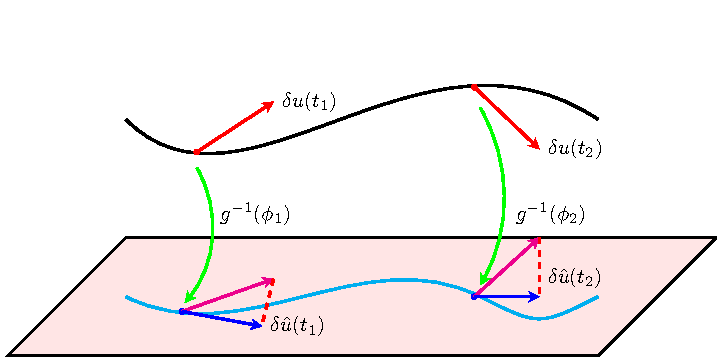
\includegraphics[width=0.9\linewidth]{jacobian_full_slice}
  \caption[Jacobian in the slice]{
    The relation between deformations in
    the full {\statesp} and in the \slice.
    The pink plane is the slice. The black curve is a trajectory in the {\statesp}.
    The cyan curve is the corresponding trajectory in the {\slice}.
    Infinitesimal deformation $\delta \ssp(t_1)$ at time $t_1$
    is transported to $\delta \ssp(t_2)$ at time $t_2$.
    $\delta \sspRed(t_1)$ and $\delta \sspRed(t_2)$ are the in-slice
    correspondents.
  }
  \label{fig:jacobian_full_slice}
\end{figure}

First, we investigate how infinitesimal deformation is
transformed into the slice from the full \statesp.
We start from the \slice\ condition \refeq{eq:slice}.
Infinitesimal deformation $\delta \sspRed$ at $\sspRed$
should be confined to the \slice\ too, so we have a constraint
\begin{equation}
  \braket{\delta \sspRed}{\sliceTan{}}=0
  \,.
  \label{eq:constraint_dx}
\end{equation}
Here, the subscript of $\sliceTan{}$ is omitted because we assume
that there
is only one group parameter.
Taking the derivative of \refeq{eq:slice3} we get
$ \delta \ssp = \delta \LieEl(\gSpace) \sspRed + \LieEl(\gSpace)
\delta \sspRed $ which is equivalent to
\[
  \delta \sspRed=-\Lg \sspRed\delta \gSpace + \LieEl(\gSpace)^{-1}\delta\ssp
  \,.
\]
Substituting it into \refeq{eq:constraint_dx},
we get
$\braket{-\mathbf{T}\sspRed\delta \gSpace + \LieEl(\gSpace)^{-1}
\delta\ssp}{t'}=0$
which is
\begin{equation}
  \label{eq:delta_theta}
  \delta \gSpace=
  \frac{\braket{\sliceTan{}}{\LieEl(\gSpace)^{-1}\delta\ssp}}
  {\braket{\groupTan(\sspRed)}{\sliceTan{}}}
\,.
\end{equation}
Now  $\delta \sspRed$, the infinitesimal deformation in the \slice, can be
expressed by the deformation in the full {\statesp} $\delta\ssp$:
\begin{equation*}
  \ket{\delta \sspRed}
  =
  -\frac{\braket{\sliceTan{}}{\LieEl(\gSpace)^{-1}\delta\ssp}}
  {\braket{\groupTan(\sspRed)}{\sliceTan{}}}
  \ket{\groupTan(\sspRed)}
  + \LieEl(\gSpace)^{-1} \ket{\delta \ssp}
  \,,
\end{equation*}
that is,
\beq
\label{eq:variation_full_slice}
\ket{\delta \sspRed} =
\left(\matId-\frac{\ket{\groupTan(\sspRed)}\bra{\sliceTan{}}}
  {\braket{\groupTan(\sspRed)}{\sliceTan{}}} \right)
\LieEl(\gSpace)^{-1}\ket{\delta \ssp}
:=
h(\sspRed)\LieEl(\gSpace)^{-1}\ket{\delta \ssp}
\eeq
The physical interpretation of \refeq{eq:variation_full_slice} is manifest.
Infinitesimal deformation $\delta \ssp$ at $\ssp$ in the full {\statesp} is
first transformed to point $\sspRed$ by $\LieEl(\gSpace)^{-1}$ and then
projected into the {\slice} by $h(\sspRed)$ illustrated in
\reffig{fig:jacobian_full_slice}.
The matrix
\beq
\pMat(\sspRed)=
    \matId-\frac{\ket{\groupTan(\sspRed)}\bra{\sliceTan{}}}
    {\braket{\groupTan(\sspRed)}{\sliceTan{}}}
%\,.
\ee{projFullToSlice}
projects infinitesimal deformation in the full {\statesp} into the {\slice}.
It is singular and has the following properties.
\begin{itemize}
\item $h(\sspRed)\ket{\groupTan(\sspRed)}=0$ :
  any infinitesimal deformation along the group tangent direction
  at $\sspRed$ in the full {\statesp} will disappear after projection.

\item $\bra{\sliceTan{}}h(\sspRed)=0$ : any vector projected into the {\slice} will be
  perpendicular to the group tangent of the template point as expected. This
  property and the above one both prove that matrix $h(\sspRed)$ is not full-rank.

\item In-slice velocity \refeq{EqMotMFrame} turns out to be
  \[
    \velRed(\sspRed)= \vel(\sspRed)
    -\frac{\braket{\vel(\sspRed)}{\sliceTan{}}}{\braket{\groupTan(\sspRed)}{\sliceTan{}}}
    \groupTan(\sspRed)=h(\sspRed)\vel(\sspRed)
    \,.
  \]
  The velocity field is transformed by matrix $h(\sspRed)$.
\end{itemize}

Since projection matrix \refeq{projFullToSlice} is singular,
the projection
reduces the dimension of the system by one.
However, \refeq{projFullToSlice} is still expressed in
the full {\statesp}.
In practice,
we desire to work in a lower\dmn\ system after quotienting out
the continuous symmetry.
Now let's decrease the dimension of all matrices and
vectors in the {\slice} by one explicitly.
Denote
\[
  \pMat(\sspRed)=
  \begin{bmatrix}
    h_{1} \\
    h_{2} \\
    \vdots \\
    h_{n}
  \end{bmatrix}
  \,.
\]
Each $h_{i}$ is a row vector and $n$ is the dimension of the full {\statesp}.
From the second property of $h(\sspRed)$ we know that $h_{i}$ are linear
dependent: $\sliceTan{1}h_{1}+\sliceTan{2}h_{2}+\cdots +\sliceTan{n}h_{n}=0$.
Here $\sliceTan{i}$ are
components of vector $\sliceTan{}$.
Assume $t'_{\xi}\neq 0$, then
\[
h_{\xi}=\sum_{i=1,i\neq \xi}^{n}-\frac{\sliceTan{i}}{\sliceTan{\xi}}h_{i}
\]
so $h_{\xi}$ can be eliminated from $\pMat(\sspRed)$:
\[
  \pMat(\sspRed)=
  \underbrace{
    \begin{bmatrix}
      1 & & & & \\
      & 1 & & & \\
      & & \ddots & & \\
      -\frac{\sliceTan{1}}{\sliceTan{\xi}} &
      -\frac{\sliceTan{2}}{\sliceTan{\xi}} & & \cdots &
      -\frac{\sliceTan{n}}{\sliceTan{\xi}} \\
      & & & \ddots  & \\
      & & & & 1 \\
    \end{bmatrix}
  }_{n\times (n-1)}
  \underbrace{
    \begin{bmatrix}
      h_{1} \\
      \vdots \\
      h_{\xi-1} \\
      h_{\xi+1} \\
      \vdots \\
      h_{n} \\
    \end{bmatrix}
  }_{(n-1)\times n}
  := P'\pMatM(\sspRed)
  \,.
\]
The above expression is the {rank factorization}
of $h(\sspRed)$ with $\pMatM(\sspRed)$ a full-rank matrix.
The superscript of the minus sign indicates that
the matrix (vector) is $(n-1)$\dmn.
Similarly, from the {\slice} condition $\braket{\sliceTan{}}{\sspRed}=0$,
we can reduce the dimension of a
point on the {\slice} by one
\[
  \sspRed=P'\sspRedM
\]
and also reduce the dimension of an infinitesimal deformation by one
\[
  \delta \sspRed=P'\delta \sspRedM
  \,.
\]
Here, $\sspRedM$ and
$\delta \sspRedM$ are both $(n-1)$\dmn\ vectors.
\[
  \sspRedM=\transp{[\sspRed_1, \cdots, \sspRed_{\xi-1}, \sspRed_{\xi+1}, \cdots, \sspRed_{n}]}
  \,, \quad
  \delta \sspRedM= \transp{[\delta \sspRed_1, \cdots, \delta \sspRed_{\xi-1},
    \delta \sspRed_{\xi+1}, \cdots, \delta \sspRed_{n}]}
  \,.
\]
Now relation \refeq{eq:variation_full_slice} can be rewritten as:
\begin{equation}
  \label{eq:projectionReduced}
  \ket{\delta \sspRedM} = \pMatM(\sspRed)\LieEl(\gSpace)^{-1}\ket{\delta \ssp}
\end{equation}
Note that the left side of the above equation
is an $(n-1)$\dmn\ vector while the right side $\ket{\delta \ssp}$
is an $n$\dmn\ vector and the $[(n-1)\times n]$ matrix $\pMatM(\sspRed)$
is the ``projection'' operator.

%%%%%%%%%%%%%%%%%%%%%%%%%%%%%%%%%%%%%%%%%%%%%%%%%%%%%%%%%%%%%%%%%%%%%%%%
\subsection{In-slice \JacobianM }
\label{sect:sliceJac}

Now let's turn to the transformation of the \JacobianM.
In \reffig{fig:jacobian_full_slice},
there is a trajectory from $\ssp(\zeit_1)$ to $\ssp(\zeit_2)$ in the full {\statesp}.
The corresponding transformed in-\slice\ trajectory is from $\sspRed(\zeit_1)$
to $\sspRed(\zeit_2)$.
Infinitesimal deformations in the full {\statesp} and in the
{\slice}  will be evolved by the
\JacobianM\ in the full {\statesp} and in the {\slice} respectively.
\begin{eqnarray}
  \jMps\delta \ssp(t_1) & = & \delta \ssp(t_2)
                              \label{eq:sliceJ}  \\
  \hat{\jMps}\delta \sspRedM(t_1) & = &\delta \sspRedM(t_2)
                                           \label{eq:sliceJ2}
                                           \,.
\end{eqnarray}
Here, $\jMps = J^{t_2 -t_1}(\ssp(t_1), \zeit_1)$ and
$\hat{\jMps} = J^{t_2 -t_1}(\sspRedM(t_1), \zeit_1)$.
For notation simplicity, we omit all parameters of \JacobianM\
if no confusion occurs.
Substituting \refeq{eq:projectionReduced} into \refeq{eq:sliceJ2},
we get
\[
  \hat{\jMps}  \pMatM(\sspRed(t_1)) \LieEl(\gSpace_1)^{-1} \delta\ssp(t_1)=
  \pMatM(\sspRed(t_2)) \LieEl(\gSpace_2)^{-1}\delta\ssp(t_2)
  =
  \pMatM(\sspRed(t_2)) \LieEl(\gSpace_2)^{-1}\jMps\delta\ssp(t_1)
  \,.
\]
The last step above has used relation \refeq{eq:sliceJ}.
This results in
\begin{equation}
  \label{eq:relation_jacobian1}
  \hat{\jMps}\pMatM
  (\sspRed(\zeit_1))\LieEl(\gSpace_1)^{-1}=
  \pMatM(\sspRed(\zeit_2))\LieEl(\gSpace_2)^{-1}\jMps
  \,.
\end{equation}
$\hat{\jMps}$ is an $[(n-1)\times (n-1)]$ matrix as we can easily see.
The geometrical meaning of relation \refeq{eq:relation_jacobian1} is obvious
in \reffig{fig:jacobian_full_slice}. On the left side, the
infinitesimal deformation $\delta \ssp(\zeit_1)$ at $\ssp(\zeit_1)$ is
transported to the slice first,
and then projected into the \slice, after which it is
evolved by $\hat{\jMps}$ to in-slice point
$\sspRed(\zeit_2)$. On the right side, the
infinitesimal deformation $\delta \ssp(\zeit_1)$ at $\ssp(\zeit_1)$ is evolved
first to $\ssp(\zeit_2)$
by $\jMps$, then transported to the slice, and finally projected
into the \slice.

By \refeq{eq:relation_jacobian1},
the relation between {\cLvs} in the full {\statesp} and in the {\slice}
can be obtained for
physically interesting invariant subsets: \eqva, \reqva, \po s, and
\rpo s.

\paragraph{In-slice stability matrix of an \eqv}
For an \eqv\ $\ssp(\zeit_1) = \ssp(\zeit_2) := \ssp_q$, we have
$\sspRed(\zeit_1)=\sspRed(\zeit_2) :=\sspRed_q$ and
$\gSpace_{1}=\gSpace_{2} := \gSpace_q$.
Formula \refeq{eq:relation_jacobian1} becomes
\begin{equation}
  \hat{\jMps}\pMatM
  (\sspRed_q)\LieEl(\gSpace_q)^{-1}=
  \pMatM(\sspRed_q)\LieEl(\gSpace_q)^{-1}\jMps
  \,.
  \label{eq:Jeqv0}
\end{equation}
Moreover, by \refeq{eq:tangentDynamics} we have $J=e^{(t_2-t_1)A}$
for \eqva, so \refeq{eq:Jeqv0} becomes
\begin{equation}
  \hat{A} \pMatM
  (\sspRed_q)\LieEl(\gSpace_q)^{-1}=
  \pMatM(\sspRed_q)\LieEl(\gSpace_q)^{-1}A
  \,,
  \label{eq:Jeqv1}
\end{equation}
where $\hat{A}$ is the in-slice stability matrix.
\refeq{eq:Jeqv1} relates stability matrix in the \slice\ and that in the
full \statesp\ by a similarity transformation.
So
\begin{equation}
  \label{eq:Jeqv}
  \hat{\ExpaEig}_{j} = \ExpaEig_{j} \,, \quad
  \jEigvecRed[j] = \pMatM(\sspRed_q)\LieEl(\gSpace_q)^{-1} \jEigvec[j]
  \,.
\end{equation}
Here, $\hat{\ExpaEig}_{j}$ and $\ExpaEig_{j}$ are the
stability exponents in the \slice\ and in the full \statesp\ respectively.
$\hat{\jEigvec}$ and $\jEigvec$ are the corresponding eigenvectors.

\paragraph{In-slice stability matrix of a \reqv}
For an \reqv\ $\LieEl(c(\zeit_2-\zeit_1)) \ssp(\zeit_2) =  \ssp(\zeit_1)$,
we also have $\sspRed(\zeit_1)=\sspRed(\zeit_2) :=\sspRed_q$ and
$\gSpace_{1} = \gSpace_{2} - c (\zeit_2 - \zeit_1)$. Formula
\refeq{eq:relation_jacobian1} reduces to
\begin{equation}
  \hat{\jMps} \left( \pMatM(\sspRed_q)\LieEl(\gSpace_1)^{-1} \right) =
  \left( \pMatM(\sspRed_q)\LieEl(\gSpace_1)^{-1} \right)
  \LieEl(c(t_2-t_1))^{-1}\jMps
  \,.
  \label{eq:Jreqv0}
\end{equation}
If let $\zeit_2 - \zeit_1 = \delta \zeit$ be an infinitesimal time
lapse. Then
\[
  \jMps = \matId + A \delta \zeit \,\quad
  \text{and} \quad
  \LieEl(c(\zeit_2 - \zeit_1)) = \matId + c\Lg \delta\zeit
\]
are
first-order accurate. Thus \refeq{eq:Jreqv0} gives
\begin{equation}
  \label{eq:Jreqv1}
  \hat{A} \left( \pMatM(\sspRed_q)\LieEl(\gSpace_1)^{-1} \right) =
  \left( \pMatM(\sspRed_q)\LieEl(\gSpace_1)^{-1} \right)
  (-c\Lg + A)
  \,.
\end{equation}
Actually, $-c\Lg + A$ is the \emph{effective} stability matrix of
a \reqv\ in the full \statesp, so \refeq{eq:Jreqv1}
relates the stability matrix in the \slice\ with the effective stability matrix
in the full \statesp\ by a similarity transformation. Therefore,
their spectra and eigenvectors have the same relation as in
\refeq{eq:Jeqv}.

\paragraph{In-slice \JacobianM\ of a \po}
For a \po\ $\ssp(0)=\ssp(\period{p})$, if we
set $\zeit_2 = \zeit_1 + \period{p}$ we have
$\sspRed(\zeit_1)=\sspRed(\zeit_2) :=\sspRed_p$ and
$\gSpace_{1}=\gSpace_{2} := \gSpace_p$. So, the Floquet matrix
has relation
$\hat{\jMps}_p\pMatM
(\sspRed_p)\LieEl(\gSpace_p)^{-1}=
\pMatM(\sspRed_p)\LieEl(\gSpace_p)^{-1}\jMps_p$.
Therefore, the \Fv s and Floquet multipliers
in the slice and those in the full \statesp\
have the
same relation as in \refeq{eq:Jeqv}.

\paragraph{In-slice \JacobianM\ of a \rpo}
For a \rpo\
$\ssp(0)=\LieEl(\gSpace_p)\ssp(\period{p})$, if we also
set $\zeit_2 = \zeit_1 + \period{p}$ then we have
$\sspRed(\zeit_1)=\sspRed(\zeit_2):=\sspRed_p$ and
$\gSpace_1 = \gSpace_p + \gSpace_2$.
Relation \eqref{eq:relation_jacobian1} becomes
\begin{equation}
  \label{eq:Jrposlice}
  \hat{\jMps} \pMatM
  (\sspRed_p)\LieEl(\gSpace_{1})^{-1}
  = \pMatM (\sspRed_p)\LieEl(\gSpace_{1})^{-1} \jMps_p
  \,.
\end{equation}
Here $\jMps_p = \LieEl(\gSpace_p) J$ is the Floquet matrix in the full
\statesp\ for a \rpo. So the same as \po s, we have relation \refeq{eq:Jeqv}.

In summary, relation \refeq{eq:Jeqv} holds for \eqva, \reqva, \po s, and
\rpo s. The stability spectrum (Floquet spectrum) in the slice is the
same as that in the full \statesp. Eigenvectors (\Fv s)
in the full \statesp\
are first transported to the slice and then projected into the slice.
This is the exact reason that using a slice to reduce continuous symmetries
not only keeps the dynamical properties unchanged but also
simplifies the analysis.

%%%%%%%%%%%%%%%%%%%%%%%%%%%%%%%%%%%%%%%%%%%%%%%%%%%%%%%%%%%%%%%%%%%%%%%%
\subsection{An example: the \twomode\ system}

In this subsection, we use the \twomode\ system as an example to
illustrate the techniques described in the previous two subsections.
We follow Chaosbook\rf{DasBuch}
for the setup of the \twomode\ system
\bea
\dot{x}_1 &=& (\mu_1    - r^2)\,x_1 + c_1\,(x_1 x_2 + y_1 y_2)
    \,,\qquad       r^2 = x_1^2 + y_1^2
\continue
\dot{y}_1 &=& (\mu_1    - r^2)\,y_1 + c_1\,(x_1 y_2 - x_2 y_1)
\continue
\dot{x}_2 &=& x_2 +  y_2 + x_1^2 - y_1^2  + a_2 x_2 r^2
\continue
\dot{y}_2 &=& -  x_2 + y_2 + 2\,x_1 y_1  + a_2 y_2 r^2
\,.
\label{angSO2set1real}
\eea
and the choice of parameters:
\[
  \mu_1 = -2.8\,,\quad
  a_2 = -2.66\,,\quad
  c_1 = -7.75\,.
\]
Full \statesp\ points are represented as
$\ssp = \transp{(x_1, y_1, x_2, y_2)}$.
The \twomode\ system \refeq{angSO2set1real} has an \SOn{2} symmetry
\[
  \LieEl(\gSpace) \,=\,  \left(\barr{ccccc}
    \cos \gSpace  &\sin \gSpace  & 0 & 0  \\
    -\sin \gSpace  &~\cos \gSpace  & 0 & 0  \\
    0 & 0 &  \cos 2\gSpace &\sin 2\gSpace    \\
    0 & 0 &  -\sin 2\gSpace &~\cos 2\gSpace
    \earr\right)
  \,
\]
with the corresponding Lie group generator
\beq
 \Lg \,=\,   \left(\barr{ccccc}
    0  & 1 & 0  &  0   \\
    -1  &  0 & 0  &  0  \\
    0  &  0 & 0  & 2   \\
    0  &  0 & -2  &  0
    \earr\right)
  \,.
\ee{2modefLieGen}
In order to reduce this continuous symmetry,
$\slicep=\transp{(1,0,0,0)}$ is chosen as the template point the
same as that in
Chaosbook\rf{DasBuch}, and thus the resulting \slice\ condition is
\[
  \braket{\sspRed}{\sliceTan{}} = 0
  \;\text{and}\;
  \hat{x}_1 > 0
  \quad \text{with} \quad
  \sliceTan{} = \transp{(0, -1, 0, 0)}
  \,.
\]
The in-slice state is denoted as
$\sspRed = \transp{(\hat{x}_1, 0, \hat{x}_2, \hat{y}_2)}$.
Symmetry reduction is equivalent to rotating every state into
the positive real axis in the $(x_1, y_1)$ plane.

\begin{figure}[h]
  \centering
  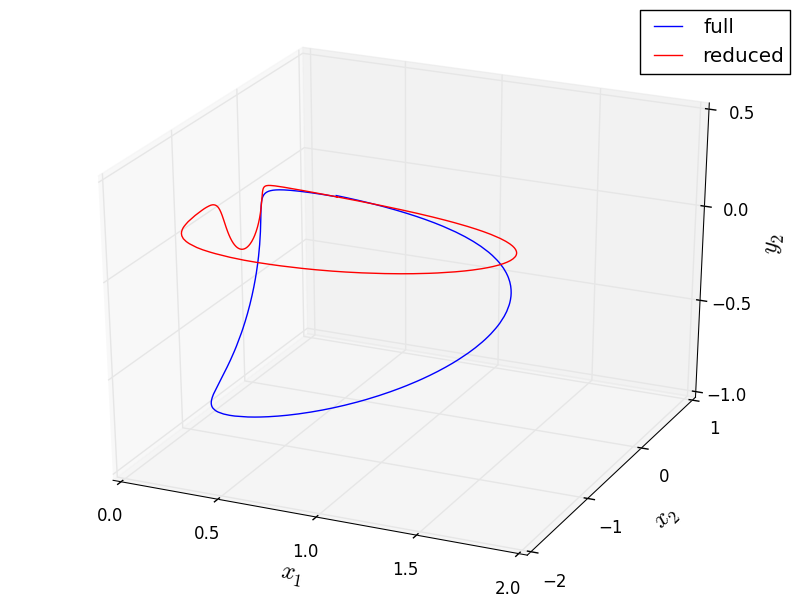
\includegraphics[width=0.8\textwidth]{twomodes_configuration}
  \caption[A \rpo\ in the \twomode\ system.]
  {
    The configuration of $\cycle{1}$ in the full \statesp\ projected
    into subspace $[x_{1},x_{2},y_{2}]$ (the blue curve) and in the slice (
    the red curve).
  }
  \label{fig:twomodes_configuration}
\end{figure}
In this subsection, we focus on one \rpo\ in the \twomode\ system
whose initial condition is
\begin{equation}
  \label{eq:2modeInit1}
  \cycle{1}: \quad (0.4525719,\quad 0.0,\quad 0.0509257,\quad 0.0335428)
  \,.
\end{equation}
The orbit has period $3.6415$.
\refFig{fig:twomodes_configuration} depicts \rpo\
$\cycle{1}$ in the full \statesp\ and in the slice.
The Floquet multipliers associated with this orbit are
\begin{equation}
  \label{eq:2modeMulti1}
  \ExpaEig_{j} : \quad (-1.481177, \quad
  -1.066888\cdot 10^{-09},\quad  0.999414,\quad  0.999913)
  \,.
\end{equation}
It has a weak expanding direction, a strong
contracting direction, and two marginal directions.

\begin{figure}[h]
  \centering
  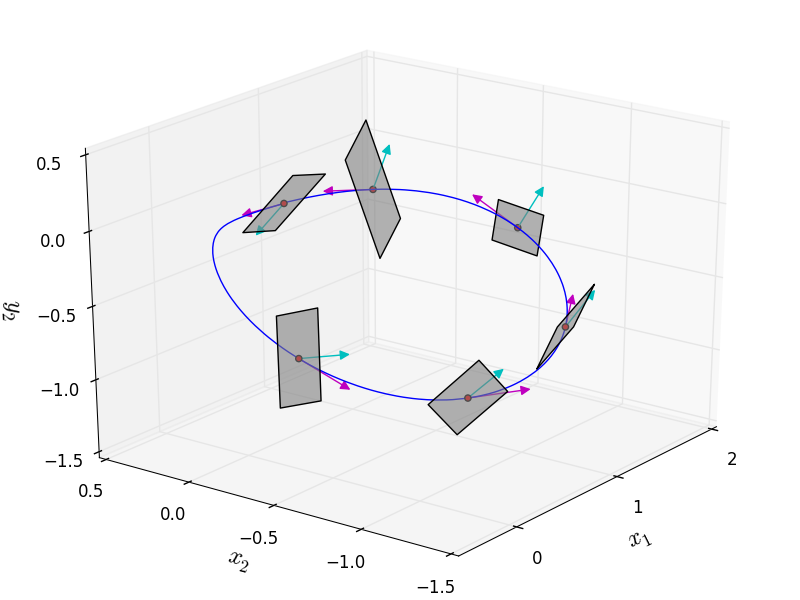
\includegraphics[width=0.8\textwidth]{twomodes_full}
  \caption[Marginal \Fv s in the \twomode\ system.]{
    The gray planes are spanned by the two marginal \Fv s.
    of \rpo\ $\cycle{1}$.
    The pink, green arrows are the velocity vectors and the group
    tangents on this orbit respectively.
    The blue curve is \rpo\ $\cycle{1}$ projected into the
    subspace $[x_{1},x_{2},y_{2}]$.
  }
  \label{fig:twomodes_full}
\end{figure}
The velocity field $\vel(\ssp)$ and the group tangent $\groupTan(\ssp)$
are \Fv s of this system and give rise to the two
marginal multipliers in \refeq{eq:2modeMulti1}, but the corresponding
two \Fv s are degenerate which cannot be told apart when we solving the
eigenequation of the \JacobianM. However, we can check whether $\vel(\ssp)$
and $\groupTan(\ssp)$ are contained in the subspace spanned by
these two \Fv s. This is the idea of \reffig{fig:twomodes_full},
in which we show the planes spanned by the two marginal \Fv s, the velocity field,
and the group tangent, along this orbit.
As we can see, $\vel(\ssp)$ and $\groupTan(\ssp)$ do lie in the planes.
Therefore, the calculation of Floquet spectrum and \Fv s
of $\cycle{1}$ is accurate at least for illustration purpose.

\begin{figure}[h]
  \centering
  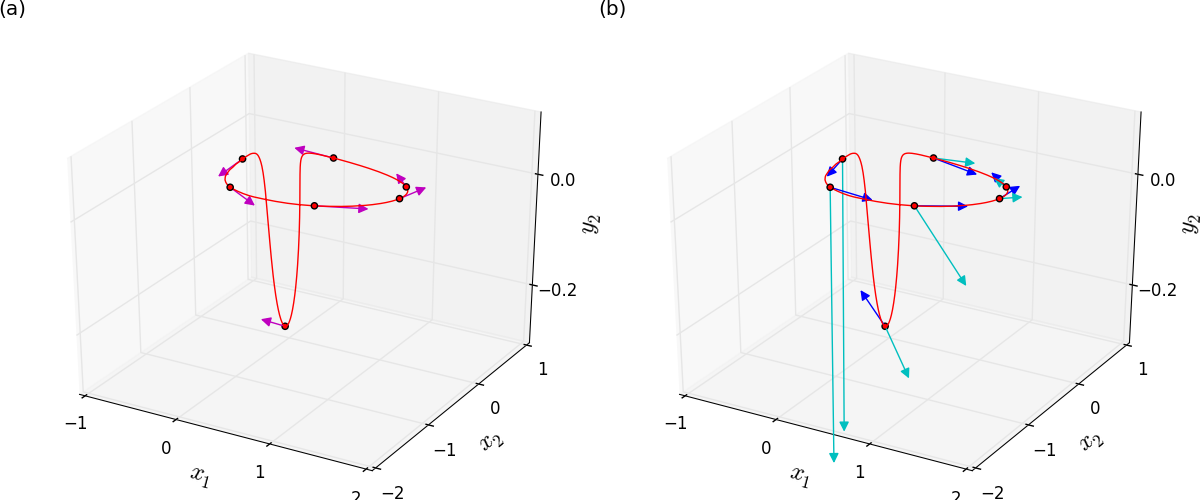
\includegraphics[width=1\textwidth]{twomodes_reduced}
  \caption[\Fv s in the slice in the \twomode\ system]{
    In-slice \Fv s for \rpo\ $\cycle{1}$.
    The red closed curve is $\cycle{1}$.
    (a) The marginal \Fv\ (pink).
    (b) The expanding (blue) and contracting (green) \Fv s in the slice.
  }
  \label{fig:twomodes_reduced}
\end{figure}

Now the task is to transform these \Fv s into the slice.
By the Lie group generator \refeq{2modefLieGen}, we get the
group tangent of an in-slice point
$\sspRed = \transp{(\hat{x}_1, 0, \hat{x}_2, \hat{y}_2)}$:
\[
  t(\sspRed)=(0,-\hat{x}_{1},2\hat{y}_{2},-2\hat{x}_{2})
  \,.
\]
Then by \refeq{projFullToSlice} we have
\[
  \pMat(\sspRed)=
  \begin{pmatrix}
    1 & 0 & 0 & 0 \\
    0 & 0 & 0 & 0 \\
    0 & 2\hat{y}_{1}/\hat{x}_{1} & 1 & 0 \\
    0 & -2\hat{x}_{2}/\hat{x}_{1} & 0 & 1 \\
  \end{pmatrix}
  \,.
\]
We choose to eliminate the second coordinate $\hat{y}_{1}$, then
\[
  \pMatM(\sspRed)=
  \begin{pmatrix}
    1 & 0 & 0 & 0 \\
    0 & 2\hat{y}_{1}/\hat{x}_{1} & 1 & 0 \\
    0 & -2\hat{x}_{2}/\hat{x}_{1} & 0 & 1 \\
  \end{pmatrix}
\,.
\]
Matrix $\pMatM(\sspRed)$ transforms \Fv s in the full \statesp\ into the
slice which are shown in \reffig{fig:twomodes_reduced}.
The group tangent $\groupTan(\sspRed)$, as one marginal vector,
disappears and the planes in \reffig{fig:twomodes_full}
collapse to the velocity
field along the orbit shown in \reffig{fig:twomodes_reduced}(a).
The other two projected \Fv s are shown in
\reffig{fig:twomodes_reduced}(b).

\begin{figure}[h]
  \centering
  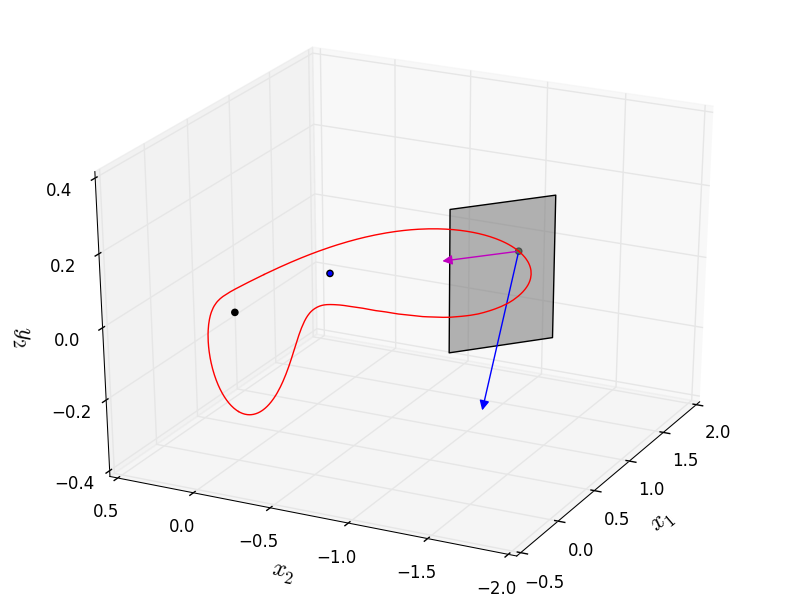
\includegraphics[width=0.8\textwidth]{twomodes_poincare}
  \caption[\Fv s on the {\PoincSec} in the \twomode\ system]{
    A vertical {\PoincSec} is constructed from the origin
    (black point) and a relative equilibrium
    (blue point) in
    the slice.
    The \PoincSec\ intersects $\cycle{1}$ (the red closed curve)
    at the green point.
    In-slice \Fv s are projected into the
    {\PoincSec}. The red/blue vector is the expanding/contracting
    \Fv. The marginal vector along the orbit disappears on the {\PoincSec}.
  }
  \label{fig:twomodes_poincare}
\end{figure}

In a similar way\rf{DasBuch}, \Fv s on
the slice could be
projected onto a {\PoincSec}. The projection matrix is
\[
  h_{\mathcal{P}}(\sspRed) = \matId -
  \frac{\ket{\hat{\vel}}\bra{\partial U}}{\braket{\hat{\vel}}{\partial U}}
  \,,
\]
where $U(x) = 0$ defines the {\PoincSec} with $\partial U$ its normal direction.
$\hat{\vel}$ is the in-slice velocity.
A \PoincSec\ can be fixed by choosing three points on it, or equivalently,
by three conditions. Here, we choose a ``vertical'' \PoincSec, namely, we demand
that the
$\hat{y}_2$ component of its normal direction vanishes. Next, this \PoincSec\
goes through the origin $(0,0,0)$ and a \reqv\
\[
  (\hat{x}_{e1}, \hat{x}_{e2},
  \hat{y}_{e2})=(0.439965,\quad -0.386267, \quad 0.070204)
  \,,
\]
shown in \reffig{fig:twomodes_poincare}.
In this case, $\partial U=(\hat{x}_{e2},- \hat{x}_{e1}, 0)$ and we get
\[
  h_{\mathcal{P}}(\sspRed)
  =\frac{1}{\hat{v}_{1}\hat{x}_{e2}-\hat{v}_{2}\hat{x}_{e1}}
  \begin{pmatrix}
    -\hat{v}_{2}\hat{x}_{e1} & \hat{v}_{1}\hat{x}_{e1} & 0 \\
    -\hat{v}_{2}\hat{x}_{e2} & \hat{v}_{1}\hat{x}_{e2} & 0 \\
    -\hat{v}_{3}\hat{x}_{e1} & \hat{v}_{3}\hat{x}_{e1} &
    \hat{v}_{1}\hat{x}_{e2}-\hat{v}_{2}\hat{x}_{e1}\\
  \end{pmatrix}
  \,.
\]
\refFig{fig:twomodes_poincare} shows the projected
expanding and contracting \Fv s
on the {\PoincSec}. The marginal vector (velocity field)
disappears.

\begin{figure}[h]
  \centering
  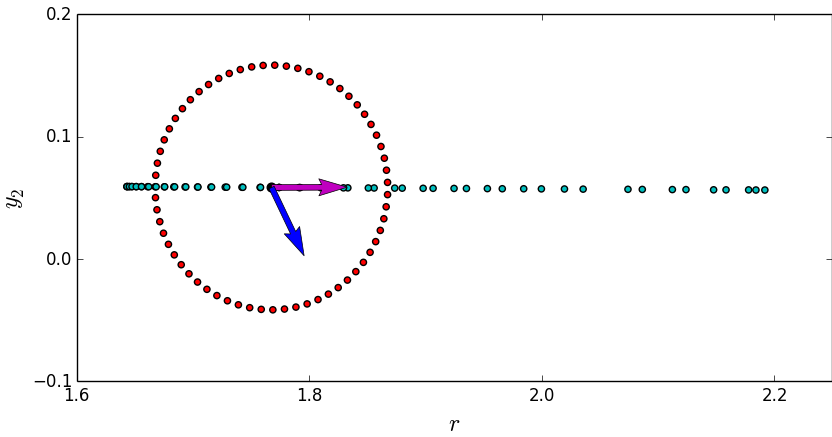
\includegraphics[width=0.8\textwidth]{twomodes_poincare_return}
  \caption[First returning points on the {\PoincSec} in
  the \twomode\ system]{
    A set of circularly (radis=0.1) distributed points (red)
    around the intersection
    point evolves for one period.
    Their first returning points (green) are recorded.
    The pink and blue arrows are the expanding
    and contracting
    \Fv s projected onto the {\PoincSec} respectively.
    Here $r=(\hat{x}_{1}^2+\hat{x}_{2}^2)^{1/2}$.
  }
  \label{fig:twomodes_poincare_return}
\end{figure}

Last, \reffig{fig:twomodes_poincare_return} shows the
{\PoincSec} and the
two projected \Fv s. A set of
circularly distributed points around
the intersection point  evolves for one period
and their first returning points are
recorded.
The contracting direction is close to the vertical direction,
and \refeq{eq:2modeMulti1} says that the contracting rate is large
in this direction. Therefore,
the returning points are squashed heavily in the
vertical direction; however, the magnitude of expanding multiplier is
about 1.5, so the elongation in the horizontal direction is relatively
small.

In summary,
we have reduced the \SOn{2} symmetry of the \twomode\ system
and discussed the \Fv s of a specific \rpo\ in the full state space and in the
slice. The marginal direction along the group orbit tangent is eliminated by the
slice. Furthermore, we have constructed a \PoincSec\ of codimension two with
respect to the original system. In this \PoincSec, the \rpo\ $\cycle{1}$
is reduced to a fixed point with
one expanding and one contracting \Fv, and the dynamics is
greatly simplified. This simple example illustrates why symmetry reduction
is an indispensable tool when studying dynamical systems with
continuous symmetries.


%% siminos/xiong/thesis/chapters/symFactor.tex
% $Author: predrag $ $Date: 2017-03-09 17:25:05 -0500 (Thu, 09 Mar 2017) $

% Xiong 2017-03-08 omitted from the thesis

\section{Discrete factorization of the dynamic zeta function}
\label{sect:fact}

When a dynamical system has a discrete symmetry, the cycle averaging
formula \refeq{eq:sd} and \refeq{eq:zeta} can be simplified substantially,
and the expansion needs
much fewer orbits to achieve the desired accuracy.
In this section, we discuss how the \dzeta\ can be factorized by a
product of contributions from each irreps of this discrete symmetry.

\subsection{Factorization of $C_3$ and $D_3$}

\begin{figure}[h]
  \centering
  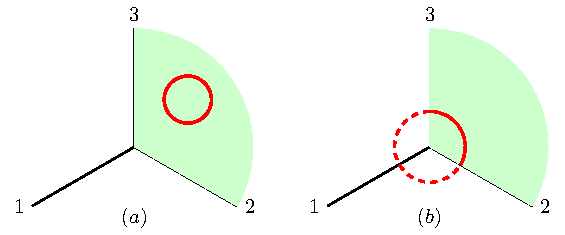
\includegraphics[width=0.9\textwidth]{C3orbits}
  \caption[Orbits in a system with $C_3$ symmetry.]{
    The two different kinds of \po s in a system with
    $C_3$ symmetry.
    The green region is the chosen fundamental domain.
    The red cycles are \po s.
  }
  \label{fig:C3orbits}
\end{figure}

$C_3$ has two subgroups $\{e\}$ and $\{e, C^{1/3}, C^{2/3}\}$, so there are
two types of \po s as shown in \reffig{fig:C3orbits}. A type-(a) orbit
has symmetry
$\{e\}$, \ie, no symmetry, and it has two replicas by rotation $C^1/3$  and $C^{2/3}$
respectively, which are not shown in this figure. So the contribution from
a type-(a) orbit to the \dzeta\ \refeq{eq:zeta} is $(1-t_p)^3$.
The cubic order refers to the a fact that there are three sibling orbits together.
Also, since the entire orbit is in the fundamental domain, we have
\[
  1/\zeta_a = (1 - t_{\hat{p}})^3
  \,.
\]
The hat on $p$ means that $t_{\hat{p}}$ is evaluated only on the part of the orbit that
is in the fundamental domain.
A type-(b) orbit is invariant under $e$, $C^{1/3}$ and $C^{2/3}$.
This orbit has no siblings and only one third
of this orbit is in the fundamental domain. The other two thirds are replicas
by rotation $C^1/3$  and $C^{2/3}$ of the part in the fundamental domain. So, its
contribution to \dzeta\ is
\[
  1/\zeta_b = 1 - t_p = 1 - t_{\hat{p}}^3
  \,.
\]
Here, relation $t_p= t_{\hat{p}}^3$ is easily obtained by its definition in
\refeq{eq:zeta}.
On the other hand, by \refexam{exam:C3regularRep},
we know that the regular representations of $e$,
$C^{1/3}$, and $C^{2/3}$ are respectively
\[
  D^{reg}(e) = %&=&
  \begin{bmatrix}
    1 & & \\
    & 1 & \\
    & & 1 \\
  \end{bmatrix} \,,  \quad
  % \continue
  D^{reg}(C^{1/3}) = %&=&
  \begin{bmatrix}
    ~ & 1 & ~\\
    ~ & ~ & 1\\
    1 & ~ & ~ \\
  \end{bmatrix}\,,  \quad
  D^{reg}(C^{2/3}) =
  \begin{bmatrix}
    ~ & ~ & 1\\
    1 & ~ & ~\\
    ~ & 1 & ~ \\
  \end{bmatrix}
  \,.
\]
You can easily verify that
\[
 (1 - t_{\hat{p}})^3 = \det(1 - D^{reg}(e)t_{\hat{p}}) \,, \quad
 1 - t_{\hat{p}}^3 = \det(1 - D^{reg}(C^{1/3})t_{\hat{p}}) =
 \det(1 - D^{reg}(C^{2/3})t_{\hat{p}})\,.
\]
Therefore, you see that the contribution from \po s to the
\dzeta\ in a system with $C_3$
symmetry are related to the regular representation of $C_3$.

\begin{figure}[h]
  \centering
  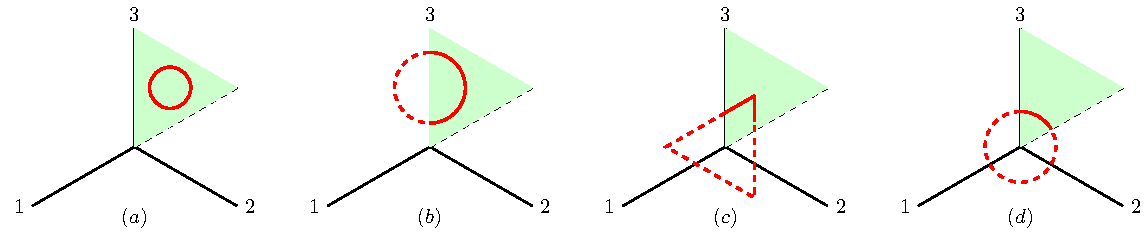
\includegraphics[width=0.9\textwidth]{D3orbits}
  \caption[Orbits in a system with $D_3$ symmetry.]{
    The four different kinds of \po s in a system with
    $D_3$ symmetry.
    The green region is the chosen fundamental domain.
    The red cycles are \po s.
  }
  \label{fig:D3orbits}
\end{figure}

Let us check out another example - a system with $D_3$ symmetry.
$D_3$ has four different kinds of subgroups $\{e\}$, $\{e, \sigma\}$,
$\{e, C^{1/3}, C^{2/3}\}$, and $D_3$ itself. Here $\sigma$ can be
any one of $\sigma_{12}$, $\sigma_{23}$ or $\sigma_{31}$. Accordingly,
there are four types of \po s as shown in \reffig{fig:D3orbits}.
The fundamental domain is one sixth of the full \statesp.
Similar to the analysis of the two orbits in the $C_3$ case, we have
\[
  1/\zeta_a = (1 - t_{\hat{p}})^6
  \,,\quad
  1/\zeta_b = (1 - t_{\hat{p}}^2)^3
  \,,\quad
  1/\zeta_c = (1 - t_{\hat{p}}^3)^2
  \,,\quad
  1/\zeta_d = 1 - t_{\hat{p}}^6
  \,.
\]
\refExam{exam:D3regularRep} gives the regular representation of $D_3$.
You can also verify that
\begin{align*}
   & (1 - t_{\hat{p}})^6 = \det(1 - D^{reg}(e)t_{\hat{p}}) \,, \quad
     (1 - t_{\hat{p}}^2)^3 = \det(1 - D^{reg}(\sigma)t_{\hat{p}}) \\
   & (1 - t_{\hat{p}}^3)^2 = \det(1 - D^{reg}(C^{1/3})t_{\hat{p}})\,,\quad
     1 - t_{\hat{p}}^6 = ?
     \,.
\end{align*}
I leave a question mark above since no analogous expression exists for it.
We will come back to it after proving
the identity \refeq{eq:symfac}.

We can generalize the above observation for a system invariant under
a general discrete group
$\Group=\{e, \LieEl_2, \LieEl_3,\cdots, \LieEl_{|\Group|}\}$.
Let $h$ be an element of $\Group$
with order (period) $m$, \ie, $m$ is the smallest positive integer such
that $h^m = e$. Then we have
\begin{equation}
  \label{eq:symfac}
  (1 - t^m)^{\frac{|G|}{m}} = \det(1 - D^{reg}(h)t)
  \,.
\end{equation}
The proof starts from the matrix identity $\ln\det = \tr\ln$, by which we have
\[
  \ln \det(1 - D^{reg}(h)t) = \tr \ln (1 - D^{reg}(h)t)
  = -\sum_{k=1}^\infty \frac{\tr D^{reg}(h^k)t^k}{k}
  \,.
\]
The last identity above comes from the Taylor expansion
$\ln(1-x) = -\sum_{k=1}^\infty \frac{x^k}{k}$.
As we know, the regular representation of
a group element has nonzero trace if and only if this group element is
$e$. So we have,
\[
  \ln \det(1 - D^{reg}(h)t) =  -\sum_{k=1}^\infty \frac{|G|t^{mk}}{mk}
  =  -\frac{|G|}{m}\sum_{k=1}^\infty \frac{t^{mk}}{k}
  = \frac{|G|}{m} \ln (1 - t^m)
  \,.
\]
Therefore, we obtain \refeq{eq:symfac}. This is why we have the observation
in the $C_3$ and $D_3$ example. However, for the type-(d) orbit in
\reffig{fig:D3orbits}, the symmetry group of this orbit is
$\{e, \sigma_{12}, \sigma_{32}, \sigma_{13}, C^{1/3}, C^{2/3}\}$. The order of
$\sigma$ is 2 while the order of $C^{1/3}$ is 3. The least common multiple is
6. Therefore, the contribution to the \dzeta\ is $(1-t_{\hat{p}}^6)^{1}$ and it
cannot be written as form $\det(1 - D^{reg}(h)t_{\hat{p}})$ with some $h\in G$.

Actually, we can write
\[
  1-t_{\hat{p}}^6 = \det(1 - D^{reg}(C^{1/3})t_{\hat{p}}^2) \,,\quad
  \text{or} \quad
  1-t_{\hat{p}}^6 = \det(1 - D^{reg}(\sigma)t_{\hat{p}}^3)
\]
With $D^{reg}(C^{1/3})$ the $[3\times 3]$ representation of $C^{1/3}$ in group $C_3$
and $ D^{reg}(\sigma)$ the $[2\times 2]$ representation of $\sigma$ in
reflection group $\{e, \sigma\}$. Anyway, for the type-(d) orbit we
have no choice but to give up the regular representation of $D_3$.

\subsection{Factorization of $C_n$ and $D_n$}

for a discrete symmetry group
$G=\{{ e},{ g}_2,\ldots,{ g}_{|G|}\}$. The orthogonality and completeness
of projection operator
can be easily verified by the orthogonality relation among characters of
irreducible representation. Define $ \cal L_\alpha=P_\alpha \cal L$, then
the trace of {\evOper} $\cal L$ can be decomposed into a sum of
$ \sum_\alpha \tr {\cal L}_\alpha$ because of the completeness of projection
operators.
\Xiong{2014-05-03}{Here the decomposition of trace just relies on the
  completeness of projection operators, we haven't used the commuting
  relation between {\evOper} and group transform. Am I right?}
So we only need to investigate the projected trace formula:
\begin{align*}
  \tr {\cal L}_\alpha & = \frac{d_\alpha}{|G|}\sum_{h \LieEl\in\Group} \chi_\alpha (h)
                        {\bf h}^{-1} \int_\pS dx \, {\cal L} ( x,x) \\
                      & =\frac{d_\alpha}{|G|}\sum_{h \LieEl\in\Group} \chi_\alpha (h) {\bf h}^{-1}
                        \sum_{a \LieEl\in\Group}\int_{\tilde{\pS}} d(a\tilde{x}) \,{\cal L} (a\tilde{x},a\tilde{x})
  \\
                      & =\frac{d_\alpha}{|G|}\sum_{h \LieEl\in\Group} \chi_\alpha (h) {\bf h}^{-1}\,\cdot
                        |G|\int_{\tilde{\pS}} d(\tilde{x}) \,{\cal L} (\tilde{x},\tilde{x}) \\
                      & = d_\alpha \sum_{h \LieEl\in\Group} \chi_\alpha (h) \int_{\tilde{\pS}} d\tilde{x} \,
                        {\cal L} ({\bf h}^{-1} \tilde{x},\tilde{x})
\end{align*}
In the above derivation, we have used the invariance of {\evOper}
under group transform. For a \po\ in the fundamental domain
$\tilde{p}$, we follow the standard argument in Chaosbook and get
\[
  \int_{\tilde{\pS}} d\tilde{x} \, {\cal L} ({\bf h}^{-1} \tilde{x},\tilde{x}) =
  \cl{\tilde{p}} \sum_{r=1}^\infty { e^{r \beta \cdot \Obser_{\tilde{p}}}
    \over  | \det \left( {\bf 1}- {\tilde\monodromy}_{\tilde{p}}^{r} \right)
    | } \delta_{n,\cl{\tilde{p}} r}\delta_{h,h_{\tilde{p}}^r}
  \,;
\]
so, the {\Fd} is
\bea
F(z) &=& \prod_\alpha F_\alpha (z)^{d_\alpha}
\continue   %\,\, , \quad \quad
F_\alpha (z) &=&
{\rm exp}  \left( - {
    \sum_{\tilde{p}} \sum_{r=1}^\infty {1 \over r}
    {\chi_\alpha (h_{\tilde{p}}^r)  z^{\cl{\tilde{p}} r}
      e^{r \beta \cdot \Obser_{\tilde{p}}}
      % {\phi_p^r}
      \over  | \det \left( {\bf 1}- {\tilde\monodromy}_{\tilde{p}}^{r} \right) | }
  } \right)
\,\,  ,
\eea
which is discrete factorization for maps. The same method can be applied to
flows with discrete symmetry:
\[
  F_\alpha (z) =
  {\rm exp}  \left( - {
      \sum_{\tilde{p}} \sum_{r=1}^\infty {1 \over r}
      {\chi_\alpha (h_{\tilde{p}}^r) e^{r (\beta \cdot \Obser_{\tilde{p}}-sT_{\tilde{p}})}
        % {\phi_p^r}
        \over  | \det \left( {\bf 1}- {\tilde\monodromy}_{\tilde{p}}^{r} \right) | }
    } \right)
\]

Making an approximation
$| \det \left( {\bf 1}- {\tilde\monodromy}_{\tilde{p}}^{r} \right) | \approx
|\Lambda_{\tilde{p}}|$ where $\Lambda_{\tilde{p}}$ is the product of all
expanding multipliers, we get the factorized zeta function:
\begin{equation}
  F_\alpha (z) =
  {\rm exp}  \left( -
    \sum_{\tilde{p}} \sum_{r=1}^\infty {1 \over r}
    \chi_\alpha (h_{\tilde{p}}^r) t_{\tilde{p}}^{r} \right)
  \label{eq:redzeta}
\end{equation}

Formula \eqref{eq:redzeta} is the ultimate goal of Discrete Factorization,
which basically tells us that,
equipped with character table of the group in question, we can write down
all the factorized zeta function for all classes of this group. On the
other hand, in order to verify our result,
let's calculate the zeta
function in the full \statesp.
\begin{align*}
  F(z) &= \prod_\alpha F_\alpha (z)^{d_\alpha} \\
       &= {\rm exp}  \left( -
         \sum_{\tilde{p}} \sum_{r=1}^\infty {1 \over r}\sum_{\alpha}
         \left(d_{\alpha}\chi_\alpha (h_{\tilde{p}}^r)\right) t_{\tilde{p}}^{r} \right) \\
       &= {\rm exp}  \left( -
         \sum_{\tilde{p}} \sum_{r=1}^\infty {1 \over r}
         |G|\delta_{h_{\tilde{p}}^{r},e}  t_{\tilde{p}}^{r} \right) \\
       &= {\rm exp}  \left( -
         \sum_{\tilde{p}} \sum_{k=1}^\infty {|G| \over mk}
         t_{\tilde{p}}^{mk} \right)
         \,,
\end{align*}
that is
\begin{equation}
  \label{eq:fullzeta}
  F(z)= \left(1-t_{\tilde{p}}^{\frac{|G|}{m}}\right)^{m} \,,
\end{equation}
where $m$ is the smallest positive number such that $h_{\tilde{p}}^{m}=e$, namely
the multiplicity of the \po\ in the full \statesp.
Formula \eqref{eq:fullzeta} is just the left side of
\beq
(1-t_{\tilde{p}}^{h_p})^{g/h_p}
=\det \left(1- D(h_{\tilde p}) t_{\tilde p} \right)
=
\prod_{\alpha} \det(1-D_{\alpha}(h_{\tilde{p}}) t_{\tilde{p}} )^{d_\alpha}
\eeq
in Chaosbook and actually formula \eqref{eq:redzeta} is the right side of
it. For completeness, I derive their equivalence here. By the
definition of character and representation of a group,
$\chi_\alpha (h_{\tilde{p}}^r)= \tr D_{\alpha}(h_{\tilde{p}}^r)
=\tr (D_{\alpha}(h_{\tilde{p}}))^{r}$ where $D$ is the regular representation
of this group, so \eqref{eq:redzeta} can be rewritten as follows,
\begin{align*}
  F_\alpha (z) & =
                 {\rm exp}  \left( -
                 \tr \sum_{\tilde{p}} \sum_{r=1}^\infty {1 \over r}
                 (D_{\alpha}(h_{\tilde{p}}))^{r} t_{\tilde{p}}^{r} \right) \\
               & ={\rm exp}  \left(
                 \tr \sum_{\tilde{p}} \ln (1-D_{\alpha}(h_{\tilde{p}}))
                 \right) \\
               & = \prod_{\tilde{p}} \det(1-D_{\alpha}(h_{\tilde{p}}))
\end{align*}
Here, we have used relation $\tr \ln= \ln \det$. All calculation of
factorized zeta function in Chaosbook is conducted by
$\det(1-D_{\alpha}(h_{\tilde{p}}))$, but I are apt to use \eqref{eq:redzeta}
because it doesn't contain information about any specific representation.
\Xiong{2014-05-05}{I am not sure whether I understand it correctly here.}
All the following examples are analyzed by \eqref{eq:redzeta}.

\paragraph{$C_{n}$} case

When $h_{\tilde p}=e$,
\[
  F_{A}=F_{\Gamma_j}={\rm exp} (-\sum_{r=1}^\infty {1 \over r}t_{\tilde{p}}^{r} )
  =1-t_{\tilde p}
  \,,
\]
Where we only investigate the contribution from one specific periodic
orbit and ignore the summation $ \sum_{\tilde{p}}$.

When $h_{\tilde p}=C_n^k$, Similarly,
\[
  F_{A}=1-t_{\tilde p}
\]
\[
  F_{\Gamma_j}={\rm exp} (-\sum_{r=1}^\infty {1 \over r}e^{\frac{i2\pi kjr}{n}}
  t_{\tilde{p}}^{r} )
  =1-e^{\frac{i2\pi kj}{n}} t_{\tilde p}
  \,,
\]
In sum,
\vskip 12pt
\begin{tabular}{rlccc}

  $h_{\tilde p}$ &  & &  $A$  &  $\Gamma_{j}$ \\
  $e$:
                 & $(1-t_{\tilde p} )^n$  &=&$(1-t_{\tilde p})$ & $(1-t_{\tilde p})$  \\
  $C_n^{k}$:
                 & $(1-t_{\tilde p}^m )^{\frac{n}{n}}$ &=&  $(1-t_{\tilde p})$ & $(1-\exp(\frac{i2\pi kj}{n})t_{\tilde p})$ \\
\end{tabular}
\vskip 12pt
\noindent


\paragraph{$C_{nv}$ ($n$ odd)} case:
When $h_{\tilde p}=e$,
\[
  F_{A_1}=F_{A_2}={\rm exp} (-\sum_{r=1}^\infty {1 \over r}t_{\tilde{p}}^{r} )
  =1-t_{\tilde p}
\]
\[
  F_{E_j}={\rm exp} (-\sum_{r=1}^\infty {2 \over r}t_{\tilde{p}}^{r} )
  =(1-t_{\tilde p})^2
\]
When $h_{\tilde p}=C_n^k$, the same goes for $A_1$ and $A_2$:
$F_{A_1}=F_{A_2}=1-t_{\tilde p}$, but for $E_j$, it requires a little
special treatment.
\begin{align*}
  F_{E_j}= & {\rm exp} (-\sum_{r=1}^\infty {1 \over r}2\cos\frac{2\pi kjr}{n}
             t_{\tilde{p}}^{r} ) \\
  = & {\rm exp} \left(-\sum_{r=1}^\infty {1 \over r}(\exp(\frac{i2\pi
      kjr}{n})+\exp(-\frac{i2\pi kjr}{n}))t_{\tilde{p}}^{r} \right) \\
  = & \left(1-\exp(\frac{i2\pi kj}{n})t_{\tilde p} \right)
      \left(1-\exp(-\frac{i2\pi kj}{n})t_{\tilde p} \right) \\
  = & 1-2\cos\frac{2\pi kj}{n}t_{\tilde p}+t_{\tilde p}^2
\end{align*}
When $h_{\tilde p}\in \{\sigma,C_n^1\sigma,\cdots,C_n^{n-1}\sigma\}$,
$h_{\tilde p}^2=e$.
\begin{align*}
  F_{A_1}= &1-t_{\tilde p} \\
  F_{A_2}= &{\rm exp} (-\sum_{r=even}^\infty {1 \over r}t_{\tilde{p}}^{r}
             +\sum_{r=odd}^\infty {1 \over r}t_{\tilde{p}}^{r} )
             =(1+t_{\tilde p}) \\
  F_{E_j}= &{\rm exp} (-\sum_{r=even}^\infty {1 \over r}2t_{\tilde{p}}^{r})
             =(1-t_{\tilde p}^2)
\end{align*}

In sum,

\vskip 12pt
\begin{tabular}{rlcccc}

  $h_{\tilde p}$ &  & &  $A_1$  &  $A_2$  &  $E_j$  \\
  $e$:
                 & $(1-t_{\tilde p} )^{2n}$  &=&$(1-t_{\tilde p})$ & $(1-t_{\tilde p})$ &
                                                                                          $ (1-t_{\tilde p})^4 $ \\
  $C_n^k,C_n^{n-k} $:
                 & $(1-t_{\tilde p}^m )^{\frac{2n}{m}}$ &=&  $(1-t_{\tilde p})$ & $(1-t_{\tilde p})$ &
                                                                                                       $ (1-2\cos(\frac{2\pi kj}{n})t_{\tilde p}+t^{2}_{\tilde p})^2 $ \\
  $\sigma,C_n^1\sigma,\cdots,C_n^{n-1}\sigma$:
                 & $(1-t_{\tilde p}^2 )^{n}$ &=&  $(1-t_{\tilde p})$ &                      $(1+t_{\tilde p})$ &$ (1-t_{\tilde p}^2)^2 $ \\
\end{tabular}
\vskip 12pt
\noindent


\paragraph{$C_{nv}$ ($n$ even)} case:
% When $h_{\tilde p}=e$, we have $F_{A_1}= %F_{A_2}=F_{B_1}=F_{B_2}=1-t_{\tilde p}$
% and $F_{E_j}=(1-t_{\tilde p})^2$
%
% When $h_{\tilde p}=C_2$, similarly, $F_{A_1}= F_{A_2}=1-t_{\tilde p}$,
% $F_{B_1}=F_{B_2}=1-(-1)^{n/2}t_{\tilde p}$ and
% $F_{E_j}=(1-(-1)^jt_{\tilde p})^2$.

Similar calculation gives us the following
factorized zeta function table.

\vskip 12pt
\begin{center}
  \begin{tabular}{b{1cm}lcccccl}

    $h_{\tilde p}$ &  & &  $A_1$  &  $A_2$  &  $B_1$  &  $B_2$  &  $E_{j}$  \\
    $e$:
                   & $(1-t_{\tilde p} )^{2n}$  &=&$(1-t_{\tilde p})$ & $(1-t_{\tilde p})$ &
                                                                                            $(1-t_{\tilde p})$ &$(1-t_{\tilde p})$&$ (1-t_{\tilde
                                                                                                                                    p})^4 $ \\
    $C_2$:
                   & $(1-t_{\tilde p}^2 )^n$ &=&  $(1-t_{\tilde p})$ & $(1-t_{\tilde p})$ &
                                                                                            $(1-(-1)^{\frac{n}{2}}t_{\tilde p})$ &$(1-(-1)^{\frac{n}{2}}t_{\tilde p})$ &
                                                                                                                                                                         $(1-(-1)^jt_{\tilde p})^4 $ \\
    $C_n^{k}$ (odd):
                   & $(1-t_{\tilde p}^m )^{\frac{2n}{m}}$ &=&  $(1-t_{\tilde p})$ & $(1-t_{\tilde p})$ &
                                                                                                         $(1+t_{\tilde p})$ &$(1+t_{\tilde p})$ &
                                                                                                                                                  $ (1-2\cos(\frac{2\pi kj}{n})t_{\tilde p}+t^{2}_{\tilde p})^2 $ \\
    $C_n^{k}$ (even):
                   & $(1-t_{\tilde p}^m )^{\frac{2n}{m}}$ &=&  $(1-t_{\tilde p})$ & $(1-t_{\tilde p})$ &
                                                                                                         $(1-t_{\tilde p})$ &$(1-t_{\tilde p})$ &
                                                                                                                                                  $ (1-2\cos(\frac{2\pi kj}{n})t_{\tilde p}+t^{2}_{\tilde p})^2 $ \\
    $\sigma$:
                   & $(1-t_{\tilde p}^2 )^n$&=& $(1-t_{\tilde p})$ & $(1+t_{\tilde p})$ &
                                                                                          $(1-t_{\tilde p})$ &$(1+t_{\tilde p})$& $ (1-t_{\tilde p}^2)^2 $ \\
    $C_n^1\sigma$:
                   & $(1-t_{\tilde p}^2 )^n$&=& $(1-t_{\tilde p})$ & $(1+t_{\tilde p})$ &
                                                                                          $(1+t_{\tilde p})$ &$(1-t_{\tilde p})$& $ (1-t_{\tilde p}^2)^2 $ \\
  \end{tabular}
\end{center}
\vskip 12pt
\noindent

When it comes to continuous symmetry, projection operator is
\beq
{P}_\eigenvG
= d_\eigenvG \int_{G} dg\,
\, \chi_\eigenvG(g^{-1})  O_g
\,.
\eeq
The corresponding trace formula in the irreducible subspace is
\beq
\sum_{\beta=0}^\infty
{1 \over \eigenvL -\eigenvL_{\eigenvG,\beta} }
=
d_\eigenvG \sum_p
\period{p}
\sum_{r=1}^\infty
\chi_\eigenvG( g_p^r)
{
  e^{r (\beta \Obser_p -\eigenvL\period{p})}
  \over
  {\left|\det\!\left(\matId-
        \tilde{\monodromy}_{\eigenvG,p}^r\right)\right|}
}
\,.
\eeq
Therefore the \Fd\ is factorized as

\bea
\det(\eigenvL - \Aop) &=& \prod_\alpha F_\alpha (z)^{d_\alpha}
\continue   %\,\, , \quad \quad
F_\alpha (z) &=&
{\rm exp}  \left( - {
    \sum_{\tilde{p}} \sum_{r=1}^\infty {1 \over r}
    {\chi_\alpha (g_{\tilde{p}}^r)  z^{\cl{\tilde{p}} r}
      e^{r \beta \cdot \Obser_{\tilde{p}}}
      % {\phi_p^r}
      \over  | \det \left( {\bf 1}- {\tilde\monodromy}_{\tilde{p}}^{r} \right) | }
  } \right)
\,\,
\eea
It differs from the discrete case on that now the group operator
$g_{\tilde{p}}$ is continuous and the factorization may have infinite terms.

\paragraph{Used formulas} Here I list several formulas used in the
above post.

\begin{equation}
  \frac{1}{2\pi}\sum_{n=-\infty}^{\infty}e^{inx} = \delta(x)
\end{equation}
This identity comes from one definition of delta function
$\delta(x)=\lim_{N\to \infty}
\frac{1}{2\pi}\frac{\sin(N+1/2)x}{\sin(\frac{1}{2}x)}$ and simple
calculation gives
$\sum_{n=-N}^{N}e^{inx}=\frac{\sin(N+1/2)x}{\sin(\frac{1}{2}x)}$.

\begin{equation}
  \sum_{R}\chi_\alpha(R) \chi_\beta(SR^{-1})=\frac{|G|}{d_\alpha}\,
  \delta _{\alpha,\beta} \chi_\alpha(S)
\end{equation}
This is the orthogonality between characters of irreducible
representations. If we set $S=e$, then it reduces to
$\sum_{R}\chi_\alpha(R) \chi_\beta(R^{-1})=|G|\delta _{\alpha,\beta}$.
The orthogonality of projection operators can be checked:
\begin{align*}
  P_\alpha P_\beta = & \frac{d_\alpha}{|G|}\, \frac{d_\beta}{|G|}
                       \sum_{h,s\LieEl\in\Group} \chi_\alpha (h) \chi_\alpha (s) {\bf h}^{-1} {\bf s}^{-1} \\
  = & \frac{d_\alpha}{|G|}\, \frac{d_\beta}{|G|} \sum_{s\LieEl\in\Group}
      \frac{|G|}{d_\alpha}\,\delta _{\alpha,\beta} \chi_\alpha(sh)(\bf{sh})^{-1} \\
  = &\delta _{\alpha,\beta} \frac{d_\alpha}{|G|}\,\sum_{s\LieEl\in\Group}
      \chi_\alpha(s){\bf s}^{-1} \\
  = & \delta _{\alpha,\beta}\, P_\alpha
\end{align*}

The last formula is
\begin{equation}
  \sum_\alpha d_\alpha \chi_\alpha (R) = |G|\, \delta_{e,R}
  \label{eq:groupcomplete}
\end{equation}
which comes from orthogonality relation above. For regular representation,
the trace of $R$ in terms of irreducible representations is
$\chi (R)=\sum_\alpha a_\alpha \chi_\alpha (R)$, so the summation of all group
elements gives
\[
  \sum_{R}\chi (R)\chi_\alpha (R^{-1})=\sum_\alpha a_\alpha \sum_{R}
  \chi_\alpha (R) \chi_\alpha (R^{-1}) =|G|\, a_\alpha
\]
On the other hand, $\chi (R)=|G|\, \delta_{e,R}$ for regular representation,
then the left side of the above expression is just $|G|\,\chi_\alpha (e)$,
so $a_\alpha =\chi_\alpha (e) =d_\alpha $ the dimension of $\alpha_{th}$
irreducible representation. In this way, we obtain \refeq{eq:groupcomplete}.
Now the completeness of projection operator can be checked:
\[
  \sum_\alpha P_\alpha = \sum_\alpha \frac{d_\alpha}{|G|} \sum_{h\LieEl\in\Group}
  \chi_\alpha (h)  {\bf h}^{-1}
  =\frac{1}{|G|} \sum_{h\LieEl\in\Group} \left(\sum_\alpha d_\alpha \chi_\alpha (h)
  \right){\bf h}^{-1}
  =e
\]


%% ======================================================================
\chapter{\KSe}
\label{chap:ks}

\section{Introduction}
\label{sect:KSintro}
    % siminos/chen/projectFall17/chapters/KSintro.txt    pdflatex project
% $Author: predrag $ $Date: 2021-01-22 16:12:00 -0500 (Fri, 22 Jan 2021) $


\KSe\ is one of the most studied models of
complex \spt\ dynamics in spatially extended systems.
It was formulated
independently by Kuramoto in the context of angular phase
turbulence in reaction-diffusion systems\rf{KurTsu75}, and
by Sivashinsky in the study of hydrodynamic instability of laminar
flames\rf{michsiv77}.
It also describes the instabilities of
dissipative trapped ion modes in plasmas\rf{laquey74} and the
flow of a viscous liquid film down a vertical wall\rf{ShSi82}.
Its one\dmn\ form is frequently written as
\begin{equation}
  u_t+\frac{1}{2}(u^2)_x+u_{xx}+u_{xxxx}=0\,,\; x\in [0,L]
  \label{eq:ks}
\end{equation}
defined on a periodic domain $u(x, t) = u(x+L, t)$.
In the combustion formulation, $u(x, t)$ represents the
flame front velocity. Everyday experience tells us that a candle flame
flickers and its shape changes quite often, without any exterior influence.
Therefore, \KSe\ is expected to exhibit chaotic behaviors.
\refFig{fig:KS_L100200} displays its \spt\ profiles with
domain size $L=100$ and $200$ respectively. Recurrent patterns appear not
only along the temporal axis but also along the spatial axis. This \spt\
chaotic behavior is also observed in other spatially-extended dynamical
systems such as \cGLe\rf{SPScgl92}.
At the same time, \reffig{fig:KS_L100200} provides coarse information about
the time and length scale of this ``dimensionless'' system.
In all our simulations, we set $L = 22$, which is large enough to exhibit
complex \spt\ chaotic dynamics{\rf{SCD07}}.

\begin{figure}
  \centering
  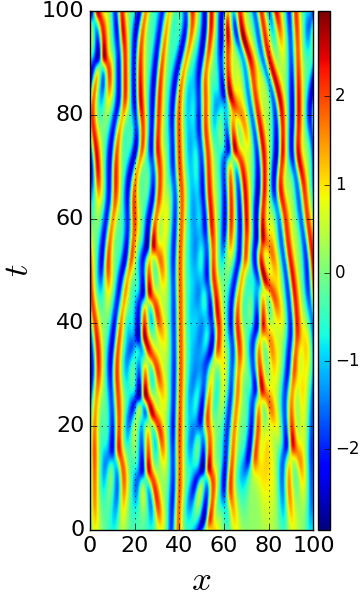
\includegraphics[height=0.35\textheight]{KS_L100N256}
  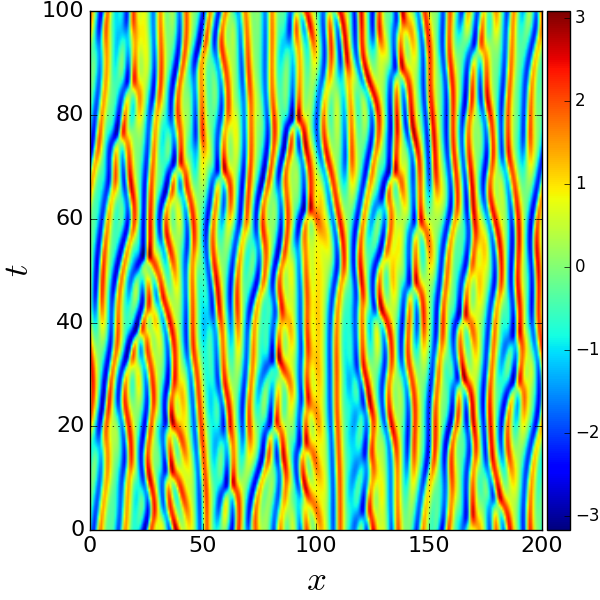
\includegraphics[height=0.35\textheight]{KS_L200N256}
  \caption[\Spt\ plots of the one\dmn\ \KSe\ for $L=100$ and $200$.]{
    Simulations of the one\dmn\ \KSe\ for domain size $L=100, 200$ respectively with random initial
    conditions. The color represents the magnitude of $u(x, t)$.
  }
  \label{fig:KS_L100200}
\end{figure}

To summarize, the form of the \KSe\ \refeq{eq:ks} on a periodic domain in one
space dimension that we use in this report is
\beq
    u_\zeit =  - u u_\conf
    -u_{\conf \conf}-u_{\conf \conf \conf \conf}
\,,\qquad
    x\in [0,L]
\,,
\ee{ACe-ks}
where subscripts denote partial derivatives.

\section{Symmetries}
\label{sect:KSsym}
    \section{Symmetries}
\label{sect:kssym}

The one\dmn\ \KSe\ has three different
symmetries. Suppose $u(x, t)$ is an orbit in this system, then we have
\begin{itemize}
\item \emph{Galilean invariance}: $u(x-ct,t)+c$ is also a
  valid orbit, where c is a constant
  number. These two orbits have different mean velocity
  $\int dx\, u$.
\item \emph{Reflection invariance}:   $-u(-x,t)$ is also a valid orbit.
  In the Fourier mode space, reflection takes form $a_k \to -a_k^{*}$.
\item \emph{Translation invariance}: $u(x+\ell,t)$ is another valid orbit.
  In the Fourier mode space, translation takes form $a_k \to e^{iq_k\gSpace} a_k$
  with $\gSpace = 2\pi \ell/L$.
\end{itemize}
The zeroth Fourier mode $a_{0}$ represents the
mean velocity of $u(x, t)$. by setting $a_{0}=0$ in the integrator,
we eliminate the Galilean symmetry.
Therefore, we only need to account for the \On{2} symmetry of this system.
Reflection in \statesp\ \eqref{eq:fourierspace} takes the form
\[
  R=\diag(-1,\, 1, \, -1, \, 1,\cdots)
  \,.
\]
The translation symmetry corresponds to an one-parameter \SOn{2}
group in the \statesp,
\[
  \LieEl(\gSpace)=\diag(r_{1},r_{2},\cdots,r_{N/2-1})
\]
with
\[
  r_{k}=
  \begin{pmatrix}
    \cos k\gSpace & \sin k\gSpace \\
    -\sin k\gSpace & \cos k\gSpace
  \end{pmatrix}
  %,\quad k=1,2,\cdots,N/2-1
  \,.
\]
The corresponding Lie group generator is
\[
  \Lg= \diag(t_{1},t_{2},\cdots,t_{N/2-1}),\quad
  t_{k}=
  \begin{pmatrix}
    0 & k \\
    -k & 0
  \end{pmatrix}
  \,.
\]
Based on the consideration of these symmetries,
there are three types of invariant orbits in \KS\ system: \po s in the
$b_k=0$ invariant antisymmetric subspace, pre\po s which are self-dual
under reflection,
and \rpo s with a shift along group orbit after one
period. As claimed in \refref{SCD07}, the first type is absent for a domain
as small as $L=22$, and thus we focus on the last two types of orbits.
\begin{itemize}
\item
  For pre\po s $\cssp(0)=R\cssp(\period{p})$ , we only need to evolve
  the system for a prime period $\period{p}$ which is half of the whole
  period. The Floquet matrix is
  $\jMps_{p}(\cssp)=R\jMps^{\period{p}}(\cssp)$.
\item
  A \rpo,
  $\cssp(0)=\LieEl_p\cssp(\period{p})$, returns after one period
  $\period{p}$ to the initial state upon the group transform
  $\LieEl_p=\LieEl(\gSpace_p)$, so the corresponding Floquet matrix is
  $\jMps_p(\cssp)=\LieEl_p\jMps^{\period{p}}(\cssp)$.
\end{itemize}
In later sections, we calculate the stability of both pre\po s
and \rpo s. We anticipate that there are two marginal directions
for both types of orbits. One marginal direction corresponds to the
velocity field and the other one is the group tangent, which is
proved in \refexam{exam:KSmarginal}.
%%%%% example start %%%%%
\exampl{
  $\vel(\cssp)$ and $\groupTan(\cssp)$ are the two marginal directions
  of both pre\po s and \rpo s}{
  \label{exam:KSmarginal}
  The \JacobianM\ transports both velocity field and group tangent along the
  flow $\jMps^{\period{p}}\vel(\cssp(0)) = \vel(\cssp(\period{p}))$,
  $\jMps^{\period{p}}\groupTan(\cssp(0)) = \groupTan(\cssp(\period{p}))$.
  Therefore, for pre\po s, we have
  $\jMps_p\vel(\cssp(0)) = R\vel(\cssp(\period{p}))
  =R\vel(R\cssp(0))$.
  Here, we have used the definition of a pre\po\ and the form of
  its Floquet matrix. By use of the equivariance relation of
  the velocity field
  under reflection $\vel(R\cssp(0)) = R\vel(\cssp(0))$, we get
  \[
    \jMps_p\vel(\cssp(0)) = R \cdot R\vel(\cssp(0)) = \vel(\cssp(0))
    \,.
  \]
  So, we see that the velocity field is one marginal direction of pre\po s
  with Floquet multiplier $1$. Similarly, for the group tangent we have
  $\jMps_p\groupTan(\cssp(0)) = R\groupTan(R \cssp(0)) =
  R \cdot \Lg \cdot R \cssp(0) $ following definition \refeq{eq:gTan}.
  Since reflection anti-commutes with rotation $R\Lg + \Lg R = 0$, then
  we have
  \[
    \jMps_p\groupTan(\cssp(0)) = -\Lg \cdot R \cdot R \cssp(0) =
    -\groupTan(\cssp(0))
    \,.
  \]
  Therefore, the group tangent is also a marginal direction of pre\po s
  but with Floquet multiplier $-1$.  A group tangent reverses direction
  after one period for pre\po s.


  For \rpo s, by a similar process we have
  \[
    \jMps_p\vel(\cssp(0)) = \LieEl_p \vel( \LieEl_p^{-1} \cssp(0)) = \vel(\cssp(0))
  \]
  and
  \[
    \jMps_p\groupTan(\cssp(0)) = \LieEl_p \groupTan( \LieEl_p^{-1} \cssp(0))
    = \groupTan(\cssp(0))
    \,.
  \]
  So, the velocity field $\vel(\cssp)$ and the group tangent  $\groupTan(\cssp)$
  are two degenerate \Fv s for \rpo s, but not degenerate for
  pre\po s.
}
%%%%% example end %%%%%
In order to reduce \On{2} symmetry, we can choose to
reduce reflection symmetry first and then translation
symmetry, or vice versa.
Note that reflection does not commute with translation
$R\LieEl(\gSpace) = \LieEl(-\gSpace)R$,
so the result of symmetry reduction depends on the order
we choose.
In this section, we elect to quotient out the \SOn{2} symmetry
by the technique described in \refsect{sec:symReduce},
more precisely, by the 1st mode slice\rf{BudCvi14}
defined by
\begin{equation}
  \label{eq:ksslice}
  c_1 = 0 ,\, b_1 >0
  \,.
\end{equation}
This corresponds to choosing
$\slicep = (1, 0,\cdots, 0)$ as the template point
in \refeq{eq:slice}.
The reduced \statesp\ is denoted as
\begin{equation}
  \label{eq:KSspred}
  \sspRed=(\hat{b}_{1}, \hat{b}_{2}, \hat{c}_{2},\cdots, \hat{b}_{N/2-1}, \hat{c}_{N/2-1})^\top
  \,.
\end{equation}
Here, $\hat{c}_{1} = 0$ is omitted explicitly.
We can rotate orbits in the full \statesp\ to
the \SOn{2}-reduced \statesp\ by transformation
$a_k \to e^{-ik\gSpace_1}a_k$ where $\gSpace_1$ is the phase of the first Fourier mode.
Alternatively, we can choose to integrate the system directly in the slice.
For a reduced \statesp\ point \refeq{eq:KSspred}, which is
a $(N-3)$-element vector, the corresponding group tangent in the full
\statesp\ is
$\groupTan(\sspRed) = (0, -\hat{b}_{1}, 2\hat{c}_{2}, -2\hat{b}_{2}, \cdots,
(N/2-1)\hat{c}_{N/2-1}, -(N/2-1)\hat{b}_{N/2-1})^\top$.
The template point is $\slicep=(1,0,\cdots,0)$;
then the corresponding group tangent is $\sliceTan{} = (0, -1, 0, \cdots, 0)$.
From \refeq{MFdtheta}
we get the dynamics in the slice
\[
  \velRed(\sspRed) = \vel(\sspRed)
  \,-\, \dot{\gSpace}(\sspRed) \groupTan(\sspRed)
  \,,\quad
  \dot{\gSpace}(\sspRed) = \frac{-\Im[\vel_1(\sspRed)] }{ \hat{b}_{1} }
  \,.
\]
When an in-slice orbit gets close to the slice border $\hat{b}_1 = 0$,
the trajectory can attain arbitrarily high speed.
To alleviate this numerical difficulty,
we rescale the time step by $dt=\hat{b}_1 d\tau$.
Thus the time-rescaled dynamics in the slice is
\begin{equation}
  \label{eq:ksRescale}
  \frac{d \sspRed}{d\tau} = \hat{b}_1 v(\sspRed) + \mathtt{Im}[v_1(\sspRed)] t(\sspRed)
  \,.
\end{equation}


\chapter{Equilibria of \KSe}
\label{chap:KSmichelson}
    \input{chapters/KSmichelson}

%\section{Invariant solutions}

Invariant structures, together with their stable and unstable
manifolds, shape the geometrical structure of the
\statesp. We also anticipate that \spt\ averages can be
calculated by \po s, as discussed in \refsect{sec:det}.
Since invariant structures play such an important role in chaotic systems,
we now discuss them in the one\dmn\
\KSe\ with $L=22$. These include \eqva, \reqva, pre\po s, and
\rpo s, whose definitions can be found in \refsect{sec:cred}.

\subsection{\Eqva\ and \reqva}

There are only three \eqva\ and two \reqva\ for domain size $L = 22$\rf{SCD07}.
They can be obtained by Newton-based numerical search such as
the Levenberg-Marquardt algorithm\rf{levenberg44, Marquardt63}
even with random initial inputs.

\begin{figure}[h]
  \centering
  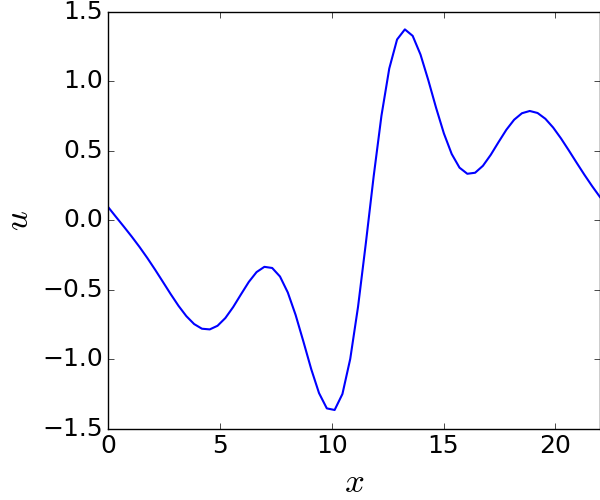
\includegraphics[width=0.32\textwidth]{ksEq1}
  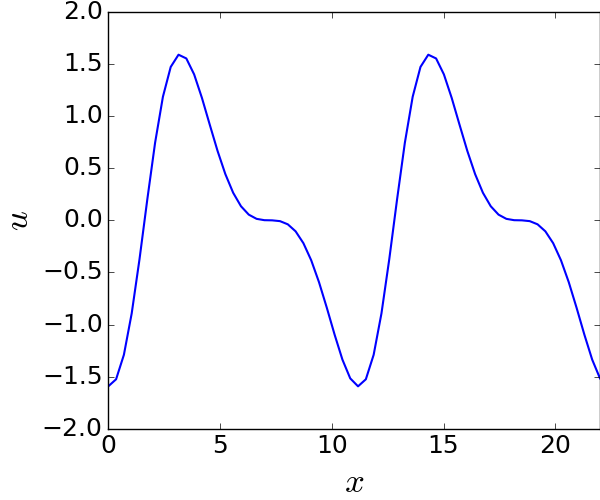
\includegraphics[width=0.32\textwidth]{ksEq2}
  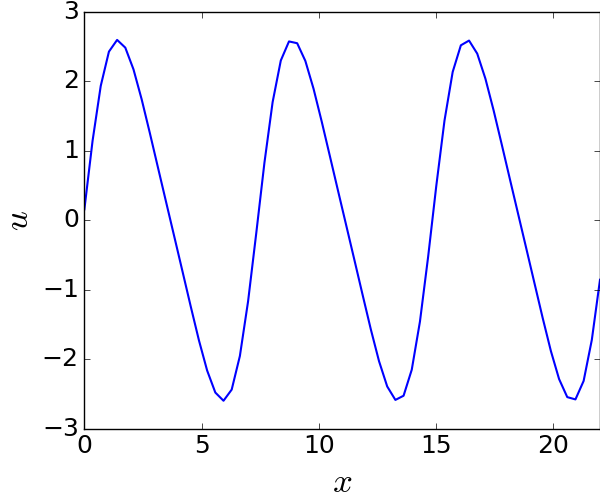
\includegraphics[width=0.32\textwidth]{ksEq3}
  \caption[Three \eqva\ in the one\dmn\ \KSe.]
  {
    Three \eqva\ \EQV{1}, \EQV{2}, and \EQV{3} from left to right in the one\dmn\ \KSe.
  }
  \label{fig:kseq}
\end{figure}

\refFig{fig:kseq} shows the profiles of these three \eqva. \EQV{1} is in
the anti-symmetric subspace $\ssp(x, t) = -\ssp(-x, t)$. \EQV{2} and
\EQV{3} are period-2 and period-3 harmonic solutions. Since $a_1 = 0$,
\EQV{2} and \EQV{3} are in the slice border.

\begin{figure}[h]
  \centering
  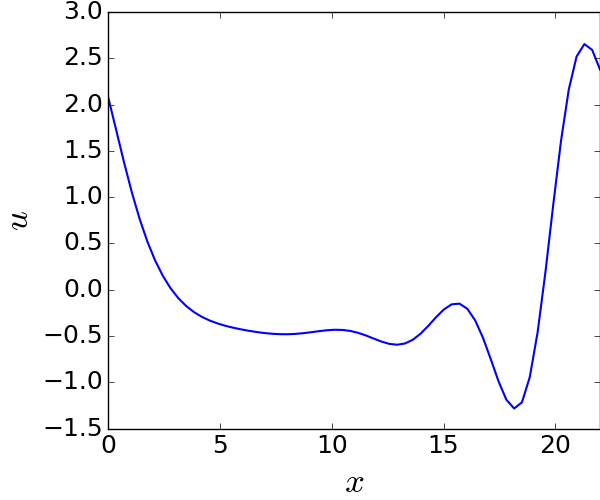
\includegraphics[width=0.45\textwidth]{ksReq1}
  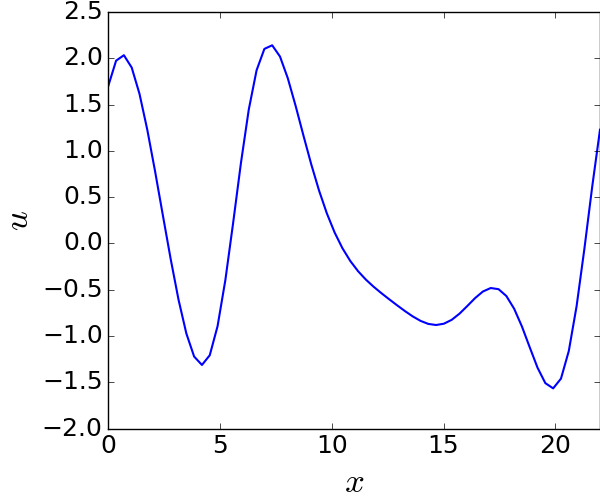
\includegraphics[width=0.45\textwidth]{ksReq2}
  \caption[Two \Reqva\ in the one\dmn\ \KSe.]
  {
    Two \reqva\ \REQV{1}{} (left) and \REQV{2}{}
    (right) in the one\dmn\ \KSe.
  }
  \label{fig:ksreq}
\end{figure}

\begin{figure}[h]
  \centering
  (a)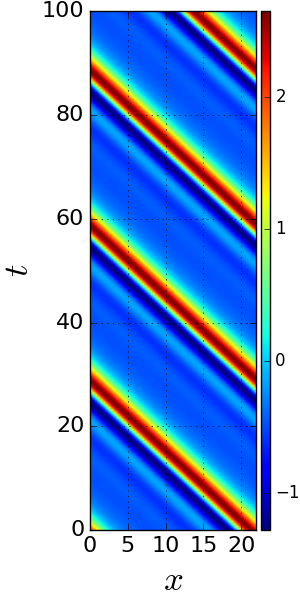
\includegraphics[width=0.2\textwidth]{ksReq1T100}
  (b)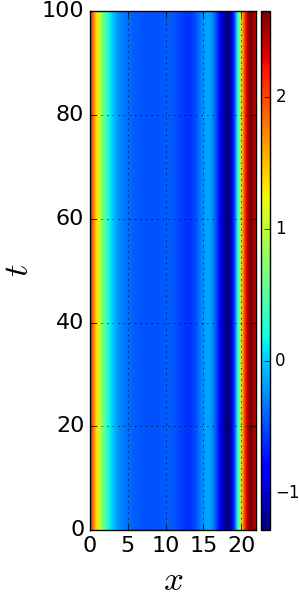
\includegraphics[width=0.2\textwidth]{ksReq1T100Red}
  (c)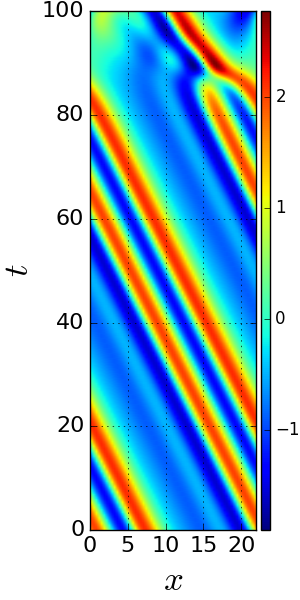
\includegraphics[width=0.2\textwidth]{ksReq2T100}
  (d)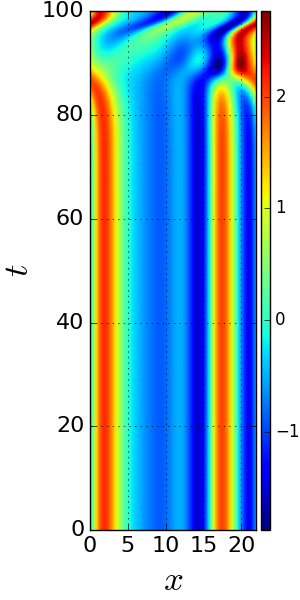
\includegraphics[width=0.2\textwidth]{ksReq2T100Red}
  \caption[\Reqva\ in the full \statesp\ and in the slice in the one\dmn\ \KSe.]
  {
    (a)(c) \REQV{1}{} and \REQV{2}{} in the full \statesp.
    (b)(d) \REQV{1}{} and \REQV{2}{} in the slice.
  }
  \label{fig:ksreqT100}
\end{figure}

\refFig{fig:ksreq} shows the profiles of the two \reqva. Their time-evolution profiles
are shown in \reffig{fig:ksreqT100}(a)(c). The color of the heat map represents $u(x, t)$.
Both of them have constant spatial translation velocity. That is why they are also called
\emph{traveling waves}. The in-slice trajectories are shown in \reffig{fig:ksreqT100}(b)(d),
in which translation symmetry has been reduced. Note, \REQV{2}{} fails to maintain its
profile after $t=80$ due to its instability. For the stability exponents of these three
\eqva\ and two
\reqva, please see\rf{SCD07}.

\subsection{Pre\po s and \rpo s}

\begin{figure}[ht]
  \centering
  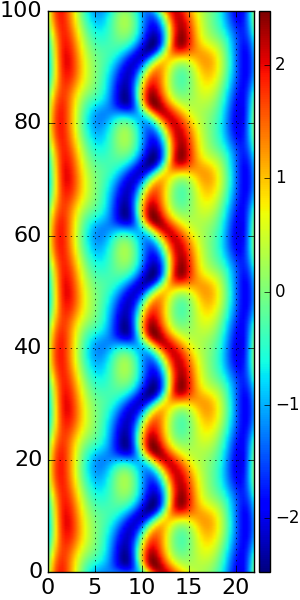
\includegraphics[width=0.16\textwidth]{ksppo1T100NoLabel}
  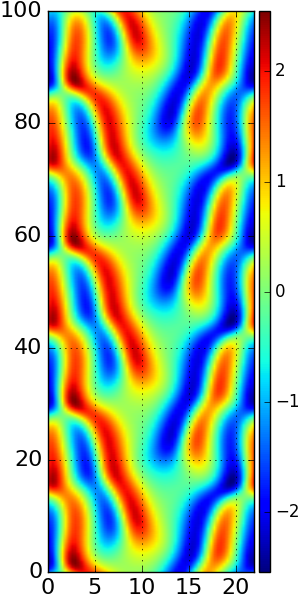
\includegraphics[width=0.16\textwidth]{ksppo2T100NoLabel}
  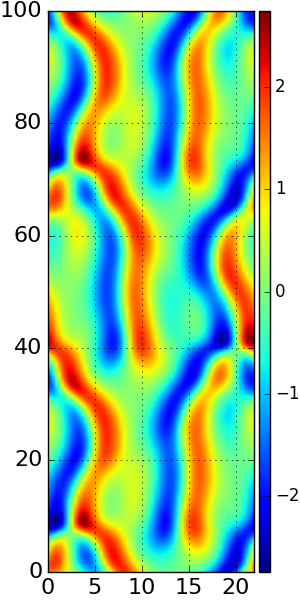
\includegraphics[width=0.16\textwidth]{ksppo3T100NoLabel}
  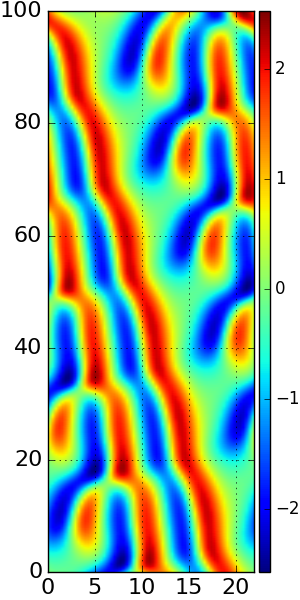
\includegraphics[width=0.16\textwidth]{ksrpo1T100NoLabel}
  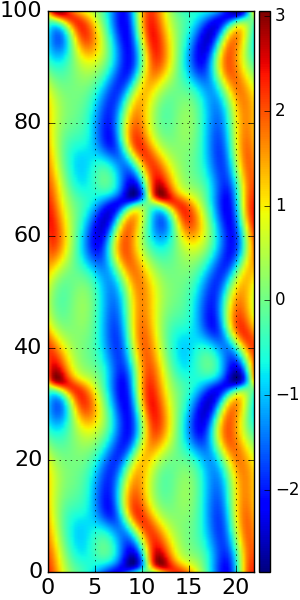
\includegraphics[width=0.16\textwidth]{ksrpo2T100NoLabel}
  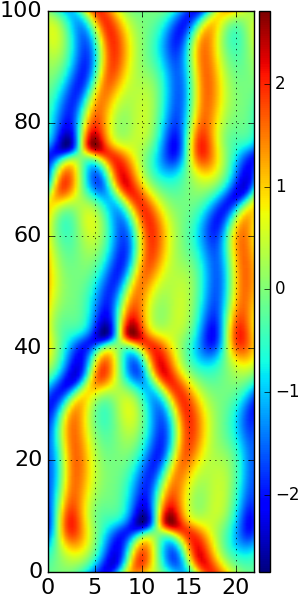
\includegraphics[width=0.16\textwidth]{ksrpo3T100NoLabel}
  \caption[Pre\po s and \rpo s in the full \statesp.]
  {
    The shortest three pre\po s and three \rpo s in the full \statesp.
    Left three: \PPO{10.25}, \PPO{14.33} and \PPO{32.36}.
    Right three: \RPO{16.31}, \RPO{32.80} and \RPO{33.50}.
  }
  \label{fig:kspoT100}
\end{figure}

\begin{figure}[ht]
  \centering
  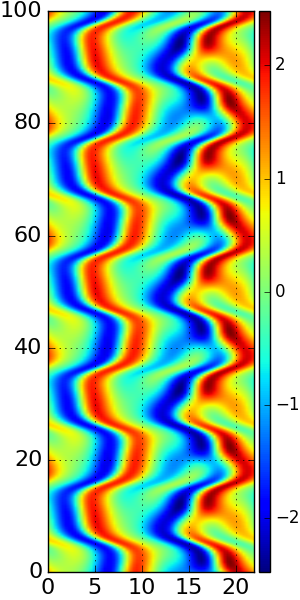
\includegraphics[width=0.16\textwidth]{ksppo1T100NoLabelRed}
  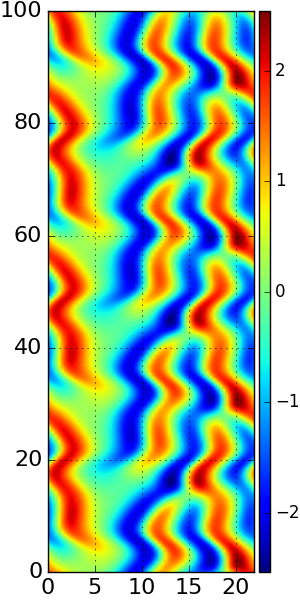
\includegraphics[width=0.16\textwidth]{ksppo2T100NoLabelRed}
  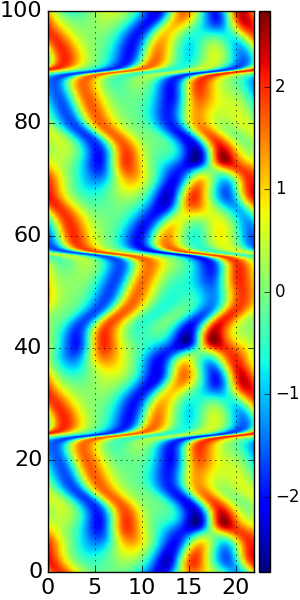
\includegraphics[width=0.16\textwidth]{ksppo3T100NoLabelRed}
  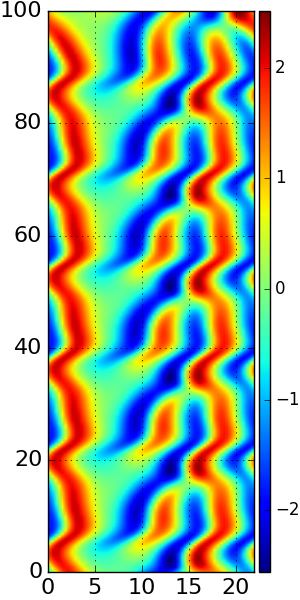
\includegraphics[width=0.16\textwidth]{ksrpo1T100NoLabelRed}
  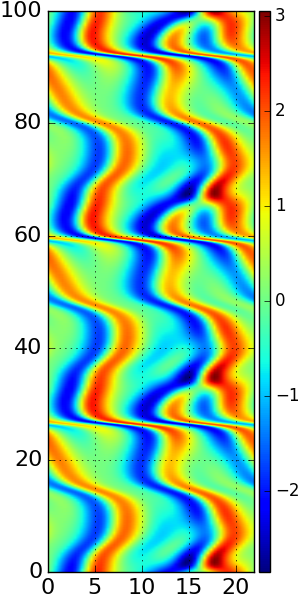
\includegraphics[width=0.16\textwidth]{ksrpo2T100NoLabelRed}
  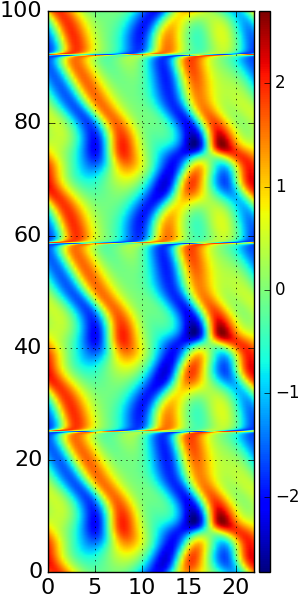
\includegraphics[width=0.16\textwidth]{ksrpo3T100NoLabelRed}
  \caption[Pre\po s and \rpo s in the slice.]
  {Orbits of \reffig{fig:kspoT100} in the slice.}
  \label{fig:kspoT100Red}
\end{figure}

Using a multishooting method, over $60\,000$ pre\po s and \rpo s\rf{SCD07} are found with
periods ranging from $10.25$ to $200$. All of them have either one or two
unstable directions. Let \PPO{T} and \RPO{T} denote the pre\po\ and \rpo\ with
period $T$ respectively. \refFig{fig:kspoT100} shows the shortest three pre\po s and
shortest three \rpo s. A pre\po\ reflects itself after one prime period, so it is
truly periodic after two prime periods. While a \rpo\ has a specific
spatial translation after each period. \refFig{fig:kspoT100Red} shows the
corresponding in-slice orbits. Since translation symmetry has been reduced,
\rpo s become periodic in the slice. Note, some of them undergo quick twists
at certain times. This is because we are using a post-processing method to transform
orbits in the full \statesp\ to the slice; therefore, when an orbit
gets close to the slice border, the rotation phase jumps sharply. If we integrate
the system directly in the slice by \refeq{eq:ksRescale}, then time will dilate when
an orbit gets close to the slice border.

\begin{table}[!ht]
  %\footnotesize
  \caption[Floquet exponents of pre\po s and \rpo s.]{
    The first 10 and last four Floquet multipliers
    $ \ExpaEig_i= \exp(\period{}\,\eigRe[i] \pm i\theta_{i})$ for
    six representative orbits.
    $\theta_{i}$ column lists either the phase,
    if the Floquet multiplier is complex, or `-1' if the
    multiplier is real, but inverse hyperbolic.
  }
  \label{tab:floquet_ppo1}
  \centering
  \begin{tabular}{l l c | l l c | l l c}
    \hline
    \multicolumn{3}{c |}{\PPO{10.25}} & \multicolumn{3}{c |}{\PPO{14.33}} & \multicolumn{3}{c}{\PPO{32.36}} \\
    \hline
    $i$ & ~~~~~$\eigRe[i]$  & $\theta_{i}$  & $i$ & ~~~~~$\eigRe[i]$ & $\theta_{i}$  & $i$ & ~~~~~$\eigRe[i]$  & $\theta_{i}$ \\
    \hline
    1,2 & ~0.033209  &    $\pm$2.0079  &     1 &          0.31095    &   -1               &     1,2&           0.064755   &  $\pm$1.9790       \\
    3 & -4.1096e-13  &                 &     2 &         -1.7825e-12 &                    &      3 &          -6.3772e-14 &                    \\
    4 & -3.3524e-14  &    -1           &     3 &          2.5049e-13 &   -1               &      4 &           1.9306e-13 &  -1                \\
    5 &  -0.21637    &                 &     4 &         -0.12154    &   -1               &      5 &          -0.17511    &                    \\
    6,7 &  -0.26524  &   $\pm$2.6205   &     5 &         -0.20150    &                    &      6 &          -0.24418    &  1                 \\
    8 &  -0.33073    &    -1           &     6 &         -0.29265    &   -1               &     7,8&          -0.27968    &  $\pm$0.6990       \\
    9 &  -1.9605    &                  &     7,8 &       -0.34313    &    $\pm$1.7872     &      9 &          -1.9868     &  -1                \\
    10 & -1.9676    &    -1            &     9 &         -1.9530    &   -1                &     10 &         -1.9891      &                    \\
       &            &                  &     10 &        -1.9928    &                     &        &                      &                    \\
       &  $\cdots$  &                  &       &         $\cdots$  &                      &        &           $\cdots$   &                    \\
    59 &  -5313.6   &    -1           &     59 &         -5312.7   &   -1                 &     59 &          -5313.3     &  -1                \\
    60 &  -5317.6   &                 &     60 &         -5318.4   &                      &     60 &          -5317.9     &                    \\
    61 &  -6051.8   &    -1           &     61 &         -6057.8   &                      &     61 &          -6052.9     &                    \\
    62 &  -6080.4   &                 &     62 &         -6074.4   &   -1                 &     62 &          -6079.2     &  -1                \\
    \hline \hline
    \multicolumn{3}{c |}{\RPO{16.31}} & \multicolumn{3}{c |}{\RPO{32.80}} & \multicolumn{3}{c}{\RPO{33.50}} \\
    \hline
    $i$ & ~~~~~$\eigRe[i]$  & $\theta_{i}$  & $i$ & ~~~~~$\eigRe[i]$ & $\theta_{i}$  & $i$ & ~~~~~$\eigRe[i]$  & $\theta_{i}$ \\
    \hline
    1 &     ~0.32791  &                  &  1,2 &      0.018610    &     $\pm$1.397964    & 1   &     0.073049   &                      \\
    2 &   ~2.8679e-12  &                 &  3   &      6.1717e-14  &                      & 2   &     0.015160   &   -1                 \\
    3 &   ~2.3559e-13  &                 &  4   &      -5.7430e-14 &                      & 3   &     1.1725e-14 &                      \\
    4 &     -0.13214  &        -1        &  5   &      -0.19688    &    -1                & 4   &    -8.8541e-14 &                      \\
    5,6 &   -0.28597  & $\pm$2.7724      &  6   &        -0.24726  &    -1                & 5   &    -0.11390    &   -1                 \\
    7 &     -0.32821  &       -1         &  7,8 &        -0.30869  &     $\pm$2.20628     & 6   &    -0.25224    &                      \\
    8 &      -0.36241  &                 &  9   &         -1.9660  &    -1                & 7,8 &    -0.26398    &   $\pm$1.0521        \\
    9,10 &   -1.9617  &  $\pm$2.2411     &  10  &         -1.9575  &    -1                & 9,10&    -1.993196   &   $\pm$0.60493       \\
         &  $\cdots$ &                   &      &         $\cdots$ &                      &     &     $\cdots$   &                      \\
    59 &   -5314.4 &                     &  59  &         -5313.9  &                      & 59  &    -5313.2     &  -1                  \\
    60 &   -5317.7 &                     &  60  &         -5317.2  &                      & 60  &    -5318.0     &  -1                  \\
    61 &   -6059.2 &                     &  61  &         -6053.9  &    -1                & 61  &    -6052.5     &                      \\
    62 &   -6072.9 &                     &  62  &         -6078.3  &    -1                & 62  &    -6079.7     &                      \\
    \hline
  \end{tabular}
\end{table}

\begin{figure}[ht]
  \centering
  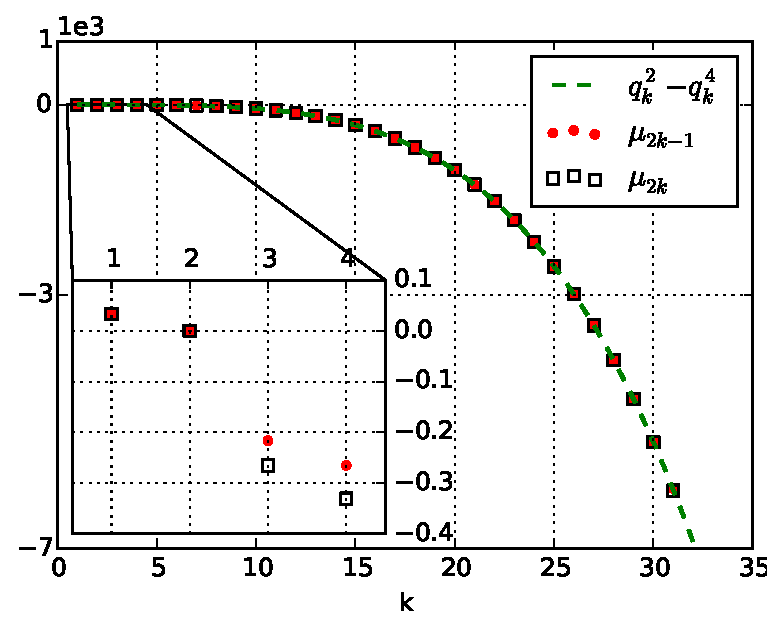
\includegraphics[width=0.6\textwidth]{ppo1spectrum64}
  \caption[Floquet spectrum of \PPO{10.25}.]{
    The real parts of the Floquet exponents paired for a given $k$ as
    $(k,\eigRe[2k-1])$ and $(k,\eigRe[2k])$ for \PPO{10.25}.
    The dashed line (green) is
    $q_{k}^{2}-q_{k}^{4}$ with $q_k = 2\pi k/L$.
    The inset is a magnification of the region
    containing the 8 leading exponents.
  }
  \label{fig:ppo1spect}
\end{figure}

This set of preperodic or relative \po s forms the backbone of the global attractor. An ergodic
trajectory shadows one orbit for a certain period and then is repelled to the neighborhood of
another orbit. This random walk is determined by the stability of the preperodic and relative
\po s.
\refTab{tab:floquet_ppo1} gives the Floquet exponents of the six orbits in \reffig{fig:kspoT100},
which are obtained by \ped\ algorithm that will be covered in \refchap{chap:ped}.
There are a few observations. First, all orbits have one or two unstable directions and
are weakly unstable. \PPO{14.33} and \RPO{16.31} are the two most unstable orbits
in our database.
% Actually, these two orbits shadow each other in the symmetry reduced
% \statesp, which will be shown in \refsect{sect:shadow}.
Second, all orbits have
two marginal directions. For pre\po s, one marginal direction has inverse hyperbolicity, \ie,
one Floquet multiplier is equal to $-1$. This was proved in \refexam{exam:KSmarginal}.
Third, the leading 8 Floquet exponents vary sharply among different orbits, but the remaining
spectrum is similar. More precisely, for large index $k$, the real parts of
Floquet exponents lie
on the curve $(q_k^2 - q_k^4 )$ as shown in \reffig{fig:ppo1spect} for \PPO{10.25}.
This means that the nonlinear term in \refeq{eq:ksfourier} is almost negligible for higher
Fourier modes, and thus they are decoupled from other modes and shrink exponentially with
rate $|q_k^2 - q_k^4 |$.
Also, Floquet exponents appear in pairs for large indices simply because
the real and complex part of high Fourier modes have a similar contraction
rate.
From these observations, we gain an intuition of how many directions
are important in shaping the neighborhood of a pre/relative \po.

%\section{\Fv s}
\label{sect:ksfv}

\Fv s are important for shaping the geometrical structure of the global
attractor in a dissipative system.
\Fv s of a pre/relative \po\ stratify the
neighborhood of this orbit. They give a rough picture of the dynamics
close to this orbit. On the other hand,
the stable and unstable manifolds of this orbit are tangent to the \Fv s,
so numerically we grow the unstable manifolds from unstable \Fv s.
Thus, \Fv s provide a way of studying the dynamics far away from this
orbit.
Calculating \Fv s is not an easy task due to the
large range of orders of expansion/contraction rates indicated by
\reftab{tab:floquet_ppo1}. However, with the invention of \ped\ algorithm
(\refchap{chap:ped}), we are able to get a full set of \Fv s at each point of a
pre/relative \po.

\begin{figure}[h]
  \centering
  \begin{minipage}{.47\textwidth}
    \centering \small{\texttt{(a)}}
    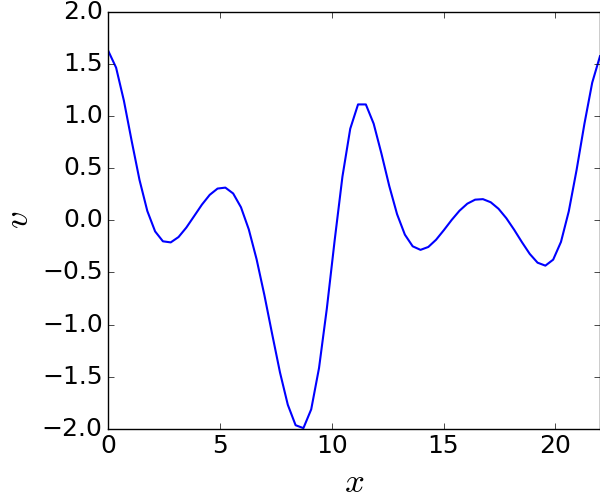
\includegraphics[width=\textwidth]{ksppo1fvt0v1r}
  \end{minipage}
  \begin{minipage}{.47\textwidth}
    \centering \small{\texttt{(b)}}
    \includegraphics[width=\textwidth]{ksppo1fvt0v5}
  \end{minipage}
  \begin{minipage}{.47\textwidth}
    \centering \small{\texttt{(c)}}
    \includegraphics[width=\textwidth]{ksppo1fvt0v10}
  \end{minipage}
  \begin{minipage}{.47\textwidth}
    \centering \small{\texttt{(d)}}
    \includegraphics[width=\textwidth]{ksppo1fvt0v30}
  \end{minipage}
  \caption[\Fv s of \PPO{10.25} at $t=0$.]{
    \Fv s of \PPO{10.25} at $t=0$ in \reffig{fig:kspoT100}.
    (a) is the real part of the 1st \Fv.
    (b), (c) and (d) are the $5$th, $10$th, and $30$th \Fv s.
  }
  \label{fig:ksfvt0}
\end{figure}

\begin{figure}[h]
  \centering
  \begin{minipage}{.115\textwidth}
    \centering \small{\texttt{(a)}}
    \includegraphics[width=\textwidth]{ppo1Fv1_64}
  \end{minipage}
  \begin{minipage}{.115\textwidth}
    \centering \small{\texttt{(b)}}
    \includegraphics[width=\textwidth]{ppo1Fv5_64}
  \end{minipage}
  \begin{minipage}{.115\textwidth}
    \centering \small{\texttt{(c)}}
    \includegraphics[width=\textwidth]{ppo1Fv10_64}
  \end{minipage}
  \begin{minipage}{.115\textwidth}
    \centering \small{\texttt{(d)}}
    \includegraphics[width=\textwidth]{ppo1Fv30_64}
  \end{minipage}
  \begin{minipage}{.115\textwidth}
    \centering \small{\texttt{(e)}}
    \includegraphics[width=\textwidth]{rpo1Fv1_64}
  \end{minipage}
  \begin{minipage}{.115\textwidth}
    \centering \small{\texttt{(f)}}
    \includegraphics[width=\textwidth]{rpo1Fv4_64}
  \end{minipage}
  \begin{minipage}{.115\textwidth}
    \centering \small{\texttt{(g)}}
    \includegraphics[width=\textwidth]{rpo1Fv10_64}
  \end{minipage}
  \begin{minipage}{.115\textwidth}
    \centering \small{\texttt{(h)}}
    \includegraphics[width=\textwidth]{rpo1Fv30_64}
  \end{minipage}%
  \caption[\Fv s of \PPO{10.25} and \RPO{16.31} for one prime period.]{
    (a) $\sim$ (d) : the 1st (real part), 5th, 10th and 30th \Fv\ along
    \PPO{10.25} for one prime period.
    (e) $\sim$ (h) : the 1st, 4th (real part), 10th (imaginary part) 30th (imaginary part)
    \Fv\ along \RPO{16.31} for one prime period.
    Axes and color scale are the same as \reffig{fig:kspoT100}.
  }
  \label{fig:Fvs}
\end{figure}
\begin{figure}[h]
  \centering
  \begin{minipage}{.47\textwidth}
    \centering \small{\texttt{(a)}}
    \includegraphics[width=\textwidth]{ppo1power64}
  \end{minipage}
  \begin{minipage}{.47\textwidth}
    \centering \small{\texttt{(b)}}
    \includegraphics[width=\textwidth]{rpo1power64}
  \end{minipage}
  \caption[The power spectrum of the first 30 \Fv s for \PPO{10.25} and \RPO{16.31}.]{
    The power spectrum of the first 30 \Fv s for \PPO{10.25}
    (left) and \RPO{16.31} (right)
    at $t=0$. Red lines correspond to the leading 8 \Fv s; while
    the blue lines correspond to the left 22 \Fv s with the $i${th} one
    localized at index $\lceil \frac{i}{2} \rceil$.
    Power at index $k$ is defined to be the square of the $k_{th}$
    Fourier coefficient's magnitude
    of \Fv s.
    The $x$-axis is
    labeled by the Fourier mode indices.
    Only the $k>0$ part is shown, and the part for
    negative $k$ follows by reflection. For complex \Fv s, the
    power spectra of the real part and imaginary part are calculated
    separately. Since almost all contracting \Fv s of \RPO{16.31}
    form complex conjugate pairs, their power peaks are far less than 1,
    as shown in panel (b).
  }
  \label{fig:FVpower}
\end{figure}

\refFig{fig:ksfvt0} shows the real part of the 1st \Fv, the 5th,
the 10th and 30th \Fv s of \PPO{10.25}. As index increases, \Fv s behave more
like pure Fourier modes.
\refFig{fig:Fvs} shows a few selected \Fv s along \PPO{10.25}
and \RPO{16.13} for one prime period respectively.
We can see that the \spt\ plots of the few leading
Fv s, see panels (a,b) and (e,f), exhibit turbulent structures containing only long waves,
for both \PPO{10.25} and \RPO{16.13},
but for
\Fv s corresponding to strong contraction rates, \ie, panels (c,d), (g,h),
the configurations
are almost pure sinusoidal curves. The power spectra in \refFig{fig:FVpower}
demonstrate this point too. The leading 8 \Fv s have large components in
the first 5 Fourier modes and the spectra are entangled with each other;
while the remaining \Fv s almost concentrate
on a single Fourier mode and are decoupled from each other;
more specifically, the $i$th \Fv\ with $i\ge 9$
peaks at the $\lceil \frac{i}{2} \rceil$th\footnote{{
Here, $\lceil x \rceil$ denotes the smallest integer no less than $x$. }}
mode in \reffig{fig:FVpower}.
Takeuchi {\etal}\rf{TaGiCh11, YaTaGiChRa08} observe similar
features in \cLv s along ergodic
trajectories and by measuring the tangency between these two groups of
\cLv s, they reach a reasonable conclusion about the dimension of
the inertial manifold in \KSe\ and \cGLe.
Therefore, we anticipate that analyzing the tangency of \Fv s along
different pre/relative \po s can also lead to the same conclusion, which
will be discussed in detail in \refchap{chap:im}.

%\section{Unstable manifolds and shadowing}
\label{sect:shadow}

Unstable manifolds of the three \eqva\ and the two \reqva,
and their connecting orbits in the full
\statesp\ have been discussed in detail in\rf{SCD07}.
With the advance in the technique of
symmetry reduction, we have a better picture of the in-slice \statesp.
Moreover, \rpo s become periodic in the slice, which helps us
organize the pre/relative \po s in our database.
In this section, we will discuss the unstable manifolds of
(relative) \eqva\ and show shadowing incidences of different orbits.

\subsection{\On{2} symmetry reduction}
\label{sect:ksO2}

\refSect{sect:kssym} introduces the 1st mode slice to reduce \SOn{2}
in the one\dmn\ \KSe. Here, we go one step further, \ie, quotienting
out reflection symmetry in the 1st mode slice.
Different from the invariant polynomial approach used by
N. B. Budanur\rf{BudanurThesis, BudCvi15}, we turn to the fundamental
domain.

In \refsect{sect:kssym}, the 1st mode slice \refeq{eq:ksslice}
is defined as the half hyperplane $c_1=0$, \ie, the imaginary
part of the 1st mode vanishes. Here, when reducing reflection in the slice,
we find it is more convenient to define the slice as
\begin{equation}
  \label{eq:ksslice2}
  b_1 = 0,\, c_1 > 0 \,,
\end{equation}
namely, we let the real part of the 1st mode vanish.
Literature\rf{BudCvi14, DCTSCD14} all chooses \refeq{eq:ksslice}.
That is why we insist on using \refeq{eq:ksslice} to define the 1st mode
slice in other chapters of this thesis.
Thus conversion \refeq{eq:ksslice2}
is only used in this section. The benefit of using \refeq{eq:ksslice2}
instead of \refeq{eq:ksslice} in this section
is that the reflection axis is parallel
to the slice \refeq{eq:ksslice2} such that the reflection rule does
not change from the full \statesp\ to the slice.
%%% example start %%%
\exampl{
  Reflection rule is invariant under \SOn{2} reduction
  by \refeq{eq:ksslice2} }{
  \label{exam:ksreflect}
  Suppose two states $\ssp_1$ and $\ssp_2$ in
  the full \statesp\
  are related to each other by reflection, $\ssp_2 = R\ssp_1$.
  Let $\sspRed_1$ and $\sspRed_2$ be their reduced states in the slice
  \refeq{eq:ksslice2}.
  If the 1st Fourier mode of $\ssp_1$ is $(b_1 + ic_1)$, then
  the 1st Fourier mode of  $\ssp_2$ is $(-b_1 + ic_1)$.
  \begin{figure}[ht]
    \centering
    \includegraphics[width=0.4\textwidth]{sliceAngle}
    \caption{Illustration of the phase relation in \refexam{exam:ksreflect}.}
    \label{fig:sliceAngle}
  \end{figure}
  So if $\LieEl(\gSpace_1)$ transforms $\ssp_1$ onto the positive
  imaginary axis in $(b_1, c_1)$ plane, that is,
  $\sspRed_1 = \LieEl(\gSpace_1) \ssp_1$, then
  $\sspRed_2 = \LieEl(-\gSpace_1) \ssp_2$ as shown in
  \reffig{fig:sliceAngle}.
  Therefore,
  \[
    \sspRed_2 = \LieEl(-\gSpace_1) R\ssp_1
    = R\LieEl(\gSpace_1) \ssp_1
    = R \sspRed_1
    \,.
  \]
  Here we have used the anti-commuting relation
  $\LieEl(-\gSpace) R = R\LieEl(\gSpace)$. So we see that
  the choice of slice \refeq{eq:ksslice2} keeps the reflection rule
  unchanged.
}
%%% example end %%%

The reflection operator is $R=\diag(-1,\, 1, \, -1, \, 1,\cdots)$.
Since $\hat{b}_1 =0$ in the slice, thus $\hat{b}_k$ with $k>1$ changes sign
after reflection. We define the fundamental domain in the slice as
\begin{equation}
  \label{eq:fundDomain}
  \hat{b}_2 > 0
  \,.
\end{equation}
Whenever an in-slice orbit leaves the fundamental domain, we transform
it back by reflection. With the sacrifice of allowing discontinuity,
we quotient out \On{2} symmetry in the one\dmn\ \KSe.

\subsection{Unstable manifold of \EQV{2} }

There are three \eqva\  \EQV{1}, \EQV{2} and \EQV{3} and two
\reqva\ \REQV{1}{} and \REQV{2}{} in this system.
$E_2$ and $E_3$ are symmetric under shifts by $L/2$ and
$L/3$ respectively as shown in \reffig{fig:kseq}.
As shown in\rf{SCD07}, one branch of the unstable manifold of
\EQV{1} and the unstable manifold of \EQV{3} terminate at \EQV{2}
or its symmetry-equivalent counterparts in the full \statesp.
Also, the unstable manifold of \EQV{2} is a set of
homoclinic orbits of itself.
Therefore, we believe that
\EQV{2} has a large influence on the geometrical structure
of the in-slice \statesp.

\refFig{fig:E2Wu} shows the unstable manifold of
\EQV{2} and several pre/relative \po s in the fundamental
domain projected into
some Fourier mode subspace. Since \EQV{2} and \EQV{3}
are in the {\sliceBord}, their \SOn{2} symmetry can not be
quotiented out by the 1st mode slice.
The blue and green straight lines are the group orbits of
\EQV{2} and \EQV{3} in the slice respectively. These
two lines depict the slice border in this three\dmn\ subspace.
Note, this does not mean that the unstable manifold of
\EQV{2} should also live in the slice. Actually, \EQV{2}
has one pair of unstable complex conjugate stability
eigenvectors, which
do have nonzero first Fourier mode components. Hence,
the corresponding unstable manifolds have unique locations,
determined by the first Fourier mode phase of this pair of
eigenvectors, in the symmetry reduced \statesp.

\begin{figure}[!ht]
  \centering
  (a)\includegraphics[width=0.8\textwidth]{ppo8}
  (b)\includegraphics[width=0.8\textwidth]{rpo3}
  \caption[The unstable manifold of \EQV{2}.]{
    The unstable manifold of \EQV{2} in the fundamental domain in the
    slice.
    The dense set of thin curves is the unstable
    manifold of \EQV{2}.
    The blue and green straight lines are the group orbits of
    \EQV{2} and \EQV{3} respectively.
    \texttt{ppo2} is \PPO{14.33} in \reffig{fig:kspoT100}.
    \texttt{rpo1} is \RPO{16.31}.
    \texttt{ppo8} is \PPO{41.08}. \texttt{rpo3} is \RPO{33.50}.
    Projection axes are the imaginary parts of the first 3 Fourier modes
    $[v_1, v_2, v_3] = [\hat{c}_1, \hat{c}_3, \hat{c}_2]$.
    This set is invariant under reflection.
  }
  \label{fig:E2Wu}
\end{figure}

There are a few interesting observations in \reffig{fig:E2Wu}.
First, the pre/relative \po s look continuous,
but in fact, they are discontinuous in the fundamental domain.
We choose the three\dmn\ subspace to be $(\hat{c}_1, \hat{c}_3, \hat{c}_2)$
which is invariant under reflection. Thus reflection has no effect
on this specific projection. Second,
the unstable manifold of \EQV{2} is discontinuous.
Whenever it crosses the slice border, there is a phase jump by $\pi$,
which causes $\hat{c}_3$ to change sign. Third, we can see that both
\texttt{ppo8} (\PPO{41.08}) and \texttt{rpo3} (\RPO{33.50}) shadow
the unstable manifold of \EQV{2} for a certain period of time.
Actually, there are plenty of
pre/relative \po s in our database that shadow
the unstable manifold of \EQV{2}.
In this sense, \EQV{2} plays a substantial role in shaping  the dynamics.

\subsection{Shadowing among orbits}

\begin{figure}[!ht]
  \centering
  (a)\includegraphics[width=0.8\textwidth]{rpo1rpo5rpo22Im}
  (b)\includegraphics[width=0.8\textwidth]{ppo24}
  \caption[Shadowing among pre/relative \po s]{
    Shadowing among pre/relative \po s in the fundamental domain.
    The dense set of thin curves is the unstable
    manifold of \EQV{2}. The two  straight lines are the group orbits of
    \EQV{2} and \EQV{3} respectively.
    Projection axes are the imaginary parts of the first 3 Fourier modes
    $[v_1, v_2, v_3] = [\hat{c}_1, \hat{c}_3, \hat{c}_2]$.
    This set is invariant under reflection.
    (a)
    The three \rpo s are (red) \RPO{16.31}, (blue) \RPO{35.97}
    and (black) \RPO{57.59}.
    (b)
    The red pre\po\ is \texttt{ppo2} (\PPO{14.33}).
    The black pre\po\ is \texttt{ppo24} (\PPO{57.67}).
  }
  \label{fig:shadow}
\end{figure}

In \reffig{fig:E2Wu}, we see that \texttt{ppo2} (\PPO{14.33})
is quite similar to \texttt{rpo1} (\RPO{16.31}). Actually,
these two orbits shadow each other and have similar
periods. There are a lot of other shadowing incidences between
different pre/relative \po s. For example, in
\reffig{fig:shadow}(a), \RPO{57.59} shadows \RPO{16.31} and
\RPO{35.97} closely. The period of this longer orbit is close to the
sum of the periods of the two shorter orbits. In \reffig{fig:shadow}(b),
\PPO{57.67} shadows \PPO{14.33} for a certain period of time.
Shadowing helps us classify all the
pre/relative \po s and helps build the symbolic
dynamics of this system. This is important for the \Fd\
\refeq{eq:sd} to converge quickly when it is expanded by only a few short
orbits\rf{DasBuch}.

On the other hand, pre\po s and \rpo s frequently show up in pairs
in the one\dmn\ \KSe. For instance,
\RPO{57.59} in \reffig{fig:shadow}(a) and \PPO{57.67} in
\reffig{fig:shadow}(b) are such a pair.
N. B. Budanur and P. Cvitanovi\'c\rf{BudCvi15} believe that this
phenomenon comes from symmetry-breaking bifurcation as
the domain size $L$ is varied.

%
%
%%% ======================================================================
%\chapter{The inertial manifold of a \KS\ system}
%\label{chap:im}
%
%% siminos/xiong/thesis/chapters/KSimintro.tex
% $Author: xiong $ $Date: 2017-03-03 18:13:05 -0500 (Fri, 03 Mar 2017) $


As stated in \refsect{sect:diss},
dynamics in chaotic dissipative systems is expected to land, after a
transient period of evolution, on the inertial
manifold\rf{constantin_integral_1989,infdymnon,temam90,Foias1988a,Robinson1995},
which is a finite\dmn\ object in \statesp. 
This is true even for infinite\dmn\ systems described by partial
differential equations, and offers hope that their asymptotic dynamics
may be represented by a finite set of ordinary differential equations.

The existence of a finite\dmn\
inertial manifold has been established for systems such as the
\KS, the \cGL, and some reaction-diffusion
systems\rf{infdymnon}. For the \NS\ flows its
existence remains an open problem\rf{temam90},
but dynamical studies, such as the determination of sets of \po s embedded in
turbulent flows\rf{GHCW07,WiShCv15}, strengthen the case for a geometrical
description of turbulence.

In this chapter, we discuss the existence and the dimension
of the global attractor and
the inertial manifold for a particular one\dmn\ \KS\ system,
defined on a ``minimal domain''.
Our discussion has two parts. In \refsect{sect:ksrb},
we review the mathematical proof of the existence of a global attractor and
the rigorous bounds for the dimension of the inertial manifold.
In \refsect{sect:ksdim}, we determine the dimension of the inertial manifold
by the numerical study of \Fv s along pre/relative \po s for this particular system.

%\section{The existence of an inertial manifold}
\label{sect:ksrb}


As discussed in \refsect{subsec:IM}, an inertial manifold is the graph of a map
$\Phi : P_n\pS \mapsto Q_n\pS$, where $P_n$ is the projection to the eigenspace spanned
by the eigenvectors of $\partial_{xx} + \partial_{xxxx}$,
corresponding to its smallest $n$ eigenvalues. $\partial_{xx} + \partial_{xxxx}$
has eigenvalues $-q_k^2+q_k^4$ with
Fourier modes as eigenvectors. Thus the existence of an inertial manifold indicates that
a finite number of \lowFmode s can describe the asymptotic behavior
of this system. Any trajectory will be attracted to this manifold exponentially fast.
This expectation is also reflected in \refeq{eq:ksfourier}, where the velocity field
of a \highFmode, \ie, $a_k$ with large $k$, is dominated by the linear
part $( q_k^2 - q_k^4 )\, a_k$. Thus, \highFmode s are almost decoupled from other modes.

An inertial manifold exists in a system which possesses the \emph{strong squeezing property}
\eqref{eq:ssp1}--\eqref{eq:ssp4}. As shown in Theorem \ref{them:spectGap}, as long as
the spectrum of $\partial_{xx} + \partial_{xxxx}$ has a sufficiently large gap for some $n$,
then an inertial manifold exists. The $k$th eigenvalue of $\partial_{xx} + \partial_{xxxx}$
is $\lambda_k = -q_k^2+q_k^4$. so $\lambda_{n+1} - \lambda_n$ is unboundedly increasing
with respect to $n$. In one\dmn\ \KSe\ \refeq{eq:ks}, the nonlinear part of the velocity
field is $-uu_x$. If we can determine a Lipschitz constant $C_1$ for $-uu_x$, then surely
there is an $n$ such that $\lambda_{n+1} - \lambda_n > 4C_1$. As a result, an inertial
manifold exists.

\emph{Strong squeezing property} has been shown to hold for one\dmn\ \KSe\ (Theorems 3.2 and corollary 3.7 in \rf{FNSTks88}, Theorem 4 in \rf{Robinson-PLA1994}).
Moreover, Robinson (Corollary 5 in \rf{Robinson-PLA1994}) states that if there is an
absorbing ball with radius $O(L^{\alpha})$
\footnote{
  The big-O notation:
  $f(x) = O(g(x))$ if and only if there exists a positive real number $M$ and
  a real number $x_0$ such that $|f(x)| \le M |g(x)|$ for all $x \ge x_0$.
}
in the one\dmn\ \KSe, then an inertial manifold exists with dimension bounded above
by $O(L^{3\alpha/5 + 3/2})$. Also, Theorem \ref{them:attractor} says that a global attractor
exists if an absorbing set exists in the \statesp. Therefore,
both a global attractor and an inertial manifold exist, provided the existence
of an absorbing set in the \statesp, which is a Hilbert space with
the $L^2$ norm
\[
  \norm{u}_{2} = \left(\int_{0}^L u^2 dx \right)^{1/2}
  \,.
\]


\subsection{Rigorous upper bounds}

In 1985, Nicolaenko, Scheurer and Temam\rf{NSTks85} gave the first asymptotic
boundedness of the $L^2$ norm of $u(x,t)$ in the antisymmetric subspace,
showing the existence of  an absorbing ball
$S = \{u\,:\, \norm{u}_{2} \le C L^{5/2}\}$
for antisymmetric solutions. They also show that the Hausdorff dimension of the
global attractor is bounded above by $O(L^{13/8})$.
This antisymmetric assumption was later removed by
Goodman\rf{Good94}.
The estimate was improved by Collet \etal\rf{CEEksgl93}
who extended it to the whole \statesp\ and improved the
exponent from $5/2$ to $8/5$.
In 2006, Bronski and Gammbill\rf{bronski2005} gave a better upper bound
\begin{equation}
  \label{eq:ksbound1}
  \limsup_{t\to\infty}\norm{u}_2 = O(L^{\frac{3}{2}})
  \,.
\end{equation}
All these results were obtained through the Lyapunov function approach,
the main idea of which is to find an appropriate gauge function $\Phi(x)$:
\begin{equation}
  \label{eq:gauge}
  u(x, t) = v(x,t) + \Phi(x)
  \,
\end{equation}
such that the transformed field $\norm{v(x, t)}_{2}$ is bounded.
Upper bound \refeq{eq:ksbound1} is claimed to be
the best result one can get by the Lyapunov function approach.
On the other hand, by treating \KSe\ as a perturbation of Burgers' equation,
Giacomelli and Otto\rf{GiacoOtto05} proved that
\footnote{
  The little-O notation :
  $f(x) = o(g(x))$ if and only if there exists a
  a real number $x_0$ such that $|f(x)| \le M |g(x)|$ for all $x \ge x_0$ and
  for all positive real number $M$.
}
\begin{equation}
  \label{eq:ksbound2}
  \limsup_{t\to\infty}|\!|u|\!|_2 = o(L^{\frac{3}{2}})
  \,.
\end{equation}
Later on, Otto\rf{Otto09} shows that
\[
  \limsup_{t\to\infty} \frac{1}{T}\int_0^T dt \norm{|\partial_x|^\alpha u}^2
  = O(L\cdot\ln^{10/3} L)
  \,,\qquad 1/3 < \alpha \le 2
  \,,
\]
and claims that it is the optimal bound for the one\dmn\ \KSe.
The norm of the
time-averaged fractional derivatives of $u(x,t)$ is almost
proportional to $L^{1/2}$. Bronski and Gammbill\rf{bronski2005}
also claim that $1/2$ is believed to be the best possible exponent.

Based on an upper bound of size of the attracting set, we can estimate
the dimension of the inertial manifold.
In 1988, Foias, Nicolaenko, Sell and Temam\rf{FNSTks88} gave an upper bound
$O(L^{7/2})$ for the dimension of the inertial manifold.
Better estimate $O(L^{2.46})$ is given in \refref{FNSTks85, jolly_evaluating_2000}.
Based on bound \refeq{eq:ksbound2}, the upper bound can be further
improved to $o(L^{12/5})$\rf{GiacoOtto05}.

In the remaining part of this section, we show the existence of an absorbing
ball through the Lyapunov function approach. The main result comes from
the work of Collet \etal\rf{CEEksgl93}. Though the estimate is not
optimal, it demonstrates the general process of obtaining the upper bound
by choosing an appropriate gauge function in \refeq{eq:gauge}.

\subsection{Existence of an absorbing ball}

Due to Galilean invariance of the \KSe, we impose zero mean velocity
$\int_0^L u(x,t)dx = 0$ in the \statesp. Then we state that
\begin{theorem}
  There is an absorbing ball $S$ with radius
  $C L^{8/5}$ in the one\dmn\ \KSe\ defined on a periodic domain
  $[0, L]$. Here, $C$ is a constant.
  % Namely,
  % \begin{equation}
  %   \limsup_{t\to\infty} ||u(x, t)||_{L^2} \le C L^{8/5}
  %   \,.
  %   \label{eq:ks_absorbing_radius}
  % \end{equation}
  \label{them:ks_readius}
\end{theorem}
Here, for simplicity, we only provide the proof of
theorem \ref{them:ks_readius} for the antisymmetric case.
For the full proof, please refer\rf{CEEksgl93, jolly_evaluating_2000}.
That is , we impose that both $v(x,t)$ and $\Phi(x)$ in \refeq{eq:gauge}
have period $L$ and are antisymmetric:
$v(-x, t) = -v(x, t)$, $\Phi(-x) = -\Phi(x)$.
Then rewriting \KSe\ \refeq{eq:ks} in terms of $v(x,t)$, we have
\[
  v_t  = (-\partial_x^2 - \partial_x^4)(v+\Phi) - vv_x - v\Phi_x -\Phi v_x
  -\Phi \Phi_x
  \,.
\]
Multiplying on both sides of the above equation with $v$
and integrating over the whole domain,
we get
\begin{align}
  \frac{1}{2} \partial_t \int v^2
  & = \int v(-\partial_x^2 - \partial_x^4)(v+\Phi)
    - \int v^2v_x - \int  v^2\Phi_x - \int  v\Phi v_x - \int  v\Phi \Phi_x
    \nonumber \\
  & = \int v(-\partial_x^2 - \partial_x^4)(v+\Phi)
    - 0 - \int v^2\Phi_x + \frac{1}{2}\int v^2\Phi_x - \int v\Phi \Phi_x
    \nonumber \\
  & = \int v(-\partial_x^2 - \partial_x^4)(v+\Phi)
    - \frac{1}{2}\int v^2\Phi_x - \int v\Phi \Phi_x  \,.
    \label{eq:ks_v2}
\end{align}
In the above, $\int v^2 v_x$ vanishes because of the periodic boundary condition.
From \refeq{eq:ks_v2}, we see that the evolution of $\norm{v(x,t)}_{2}^2$ depends
on the choice of the gauge function. In order to bound $\norm{v(x,t)}_{2}$, we need
to bound the right side of \refeq{eq:ks_v2} for some carefully
chosen gauge function $\Phi(x)$. Before that, we define notation
\begin{equation}
  \label{eq:ks_inner}
  (v_1, v_2)_{\gamma \Phi} = \int v_1(\partial_x^2 + \partial_x^4 + \gamma \Phi_x)v_2
  \,.
\end{equation}
Therefore, \refeq{eq:ks_v2} becomes
\begin{equation}
  \label{eq:ks_v2_new}
  \frac{1}{2} \partial_t \int v^2  = -(v, v)_{\Phi/2} -(v, \Phi)_{\Phi}
  \,.
\end{equation}
To bound the right side of \refeq{eq:ks_v2_new}, we bring up two propositions.
\begin{proposition}
  There is a constant $K$
  and an antisymmetric gauge function $\Phi(x)$ such that for
  all $\gamma\in[\frac{1}{4}, 1]$ and all antisymmetric
  $v(x, t)$ one have inequalities
  \begin{equation}
    \label{eq:ks_prop_1}
    (v, v)_{\gamma\Phi} \ge \frac{1}{4} \int(v_{xx}^2 + v^2)
    \,\quad \text{and }
  \end{equation}
  \begin{equation}
    \label{eq:ks_prop_2}
    (\Phi, \Phi)_{\gamma\Phi} \le KL^{16/5}
    \,.
  \end{equation}
  %\label{prop:ks_1} % lower letter does not show up in chapter title
  \label{PROP:KS1}
\end{proposition}
\begin{proposition}
  Definition \refeq{eq:ks_inner} defines an inner product in the $L^2$ space.
  \label{prop:ks_2}
\end{proposition}
With these two propositions, we then continue from \refeq{eq:ks_v2_new},
\begin{align}
  \frac{1}{2} \partial_t \int v^2
  & \le -(v, v)_{\Phi/2} + (v, v)_{\Phi}^{1/2} (\Phi, \Phi)_{\Phi}^{1/2}
    \label{eq:ks_v2_step1} \\
  & = -(v, v)_{\Phi/2} + \left(\epsilon (v, v)_{\Phi}\right)^{1/2}
    \left(\frac{1}{\epsilon}(\Phi, \Phi)_{\Phi}\right)^{1/2}
    \nonumber \\
  & \le -(v, v)_{\Phi/2} + \frac{\epsilon}{2}(v, v)_{\Phi} +
    \frac{1}{2\epsilon}(\Phi, \Phi)_{\Phi}
    \nonumber \\
  & = -\int v\left((1 - \frac{\epsilon}{2})(\partial_x^2 + \partial_x^4)
    + (\frac{1}{2}-\frac{\epsilon}{2})\gamma \Phi_x \right)v +
    \frac{1}{2\epsilon}(\Phi, \Phi)_{\Phi} \nonumber \\
  & = -(1 - \frac{\epsilon}{2})
    (v, v)_{\Phi(\frac{1}{2}-\frac{\epsilon}{2})/(1 - \frac{\epsilon}{2})} +
    \frac{1}{2\epsilon}(\Phi, \Phi)_{\Phi} \nonumber \\
  & \le -(1 - \frac{\epsilon}{2}) \frac{1}{4} \int(v_{xx}^2 + v^2) +
    \frac{1}{2\epsilon}(\Phi, \Phi)_{\Phi}
    \label{eq:ks_v2_step2} \\
  & \le -(1 - \frac{\epsilon}{2}) \frac{1}{4} \int v^2 +
    \frac{1}{2\epsilon}(\Phi, \Phi)_{\Phi} \nonumber
    \,.
\end{align}
We set $\epsilon = 2/3$ to make
$(\frac{1}{2}-\frac{\epsilon}{2})/(1 - \frac{\epsilon}{2}) = 1/4$, so we get
\begin{equation}
  \label{eq:ks_v2_bound}
  \partial_t \int v^2 \le -\frac{1}{3} \int v^2 + \frac{3}{2}(\Phi, \Phi)_{\Phi}
  \,.
\end{equation}
Step \refeq{eq:ks_v2_step1} has used
proposition \ref{prop:ks_2} such that Cauchy-Schwarz inequality can be
applied : $(v, \Phi)^2 \le (v, v)(\Phi, \Phi)$. Step \refeq{eq:ks_v2_step2}
has used \refeq{eq:ks_prop_1} in proposition \ref{PROP:KS1}. Derivative
of $\int v^2$ is bounded as shown in \refeq{eq:ks_v2_bound} and note that
term $\frac{3}{4}(\Phi, \Phi)_{\Phi}$ does not depend on time, so applying
lemma \ref{lem:Gronwall}, we obtain
\begin{equation}
  \label{eq:eq:ks_v2_bound2}
  \int v(x, t)^2 dx \le e^{-t/3}\int v(x, 0)^2 dx + \frac{9}{2}(1-e^{t/3})
  (\Phi, \Phi)_{\Phi}
  \,.
\end{equation}
Since $u(x, t) = v(x, t)+ \Phi(x)$, we therefore obtained an absorbing ball in the \KSe\
centered at $\Phi(x)$
with radius $\rho > \rho_0$, where
\begin{equation}
  \label{eq:ks_radius}
  \rho_0 = 3\sqrt{\frac{(\Phi, \Phi)_{\Phi}}{2}}  = O (L^{8/5})
  \,.
\end{equation}
Here, we have used relation \refeq{eq:ks_prop_2}.
Actually, Jolly, Rosa,
and Temam\rf{jolly_evaluating_2000} constructed a gauge function
such that the $L^2$ norm of $\Phi$ is bounded
$\norm{\Phi}_2 = O(L^{3/2})$. Therefore, the center of the
absorbing ball can be moved to the origin. Thus
\[
  \limsup_{t\to\infty} \norm{u(x, t)}_2 =   O(L^{8/5}) +  O(L^{3/2}) = O(L^{8/5})
  \,.
\]
As shown in \refeq{eq:ks_radius},
the radius of the absorbing ball depends on the choice of the gauge function
$\Phi(x)$. To make the radius as small as possible,
we try to minimize the exponent in \refeq{eq:ks_prop_2} and at the same time
to meet the requirement of  \refeq{eq:ks_prop_1}. This requires us to
choose the gauge function with the least norm which also supports
\refeq{eq:ks_prop_2} and proposition \ref{prop:ks_2}.
Actually, proposition  \ref{prop:ks_2} is a natural corollary of proposition
\ref{PROP:KS1}. The reason is as follows.
Apparently, the bilinear form \refeq{eq:ks_inner} satisfies
relations
$(\lambda v_1 + \mu v_2, v_3)_{\gamma \Phi} = \lambda (v_1, v_3)_{\gamma \Phi}
+ \mu (v_2, v_3)_{\gamma \Phi}$ and
$(v_1, v_2)_{\gamma \Phi} = (v_2, v_1)_{\gamma \Phi}$. In order to
make it an inner product, we only need to
demonstrate that $(v, v)_{\gamma \Phi} \ge 0$
with equality if and only if $v = 0$. Equation \refeq{eq:ks_prop_1}
provides this relation. Therefore, we only
need to prove proposition \ref{PROP:KS1}, which is given in
appendix \ref{chap:ksproof}.

%\section{Numerical evidence provided by \Fv s}
\label{sect:ksdim}

While mathematical approaches
provide rigorous bounds on dimensions of inertial manifolds, their
constructive description remains a challenge. In this section,
we provide numerical evidence that gives a specific integer dimension
of the inertial manifold inside the one\dmn\ \KSe.
We show that the
finite\dmn\ physical manifold can be precisely embedded in its
infinite\dmn\ \statesp, thus opening a path towards its explicit
construction. The key idea\rf{DasBuch} is to populate the inertial
manifold by an infinite hierarchy of unstable time-invariant solutions,
such as \po s, an invariant skeleton which, together
with the local ``tiles'' obtained by linearization of the dynamics,
fleshes out the physical manifold. Chaos can then be viewed as a walk on
the inertial manifold, chaperoned by the nearby unstable solutions
embedded in the physical manifold.
Unstable \po s have already been
used to compute global averages of spatiotemporally chaotic flows\rf{Christiansen97,lanCvit07,SCD07,GHCW07}.

In our analysis, we use 200 pre\po s and 200
\rpo s. These are the shortest \po s taken from the set of
over 60\,000 determined in \refref{SCD07} by near-recurrence searches.
The method preferentially finds orbits embedded in the long-time
attracting set but offers no guarantee that all orbits up to a given
period have been found.
There are infinitely many unstable orbits, and each of them
{possesses} infinitely many Floquet modes. While in the example that we
study here we do not have a detailed understanding of the organization of
\po s (their symbolic dynamics), we
show that one only needs to consider a finite number of
them to tile the physical manifold to a reasonable accuracy.
We also show, for the first time, that each local tangent tile spanned by
the \Fv s of an unstable \po\ splits into a set of
{\entangled} Floquet modes  and the remaining set of {\transient} modes.
Furthermore, we verify numerically that the {\entangled} Floquet manifold
coincides locally with the physical manifold determined by the covariant
Lyapunov vectors approach.


\subsection{Motivation from \cLvs}

Recent progress towards this aim came from numerical investigations of
the \cLvs\
of spatiotemporally chaotic flows\rf{YaTaGiChRa08,TaGiCh11}, made
possible by the
algorithms developed in \refrefs{ginelli-2007-99,WoSa07,GiChLiPo12}.
These works have revealed that the tangent space
of a generic spatially-extended dissipative system is split into two
hyperbolically decoupled subspaces: a finite\dmn\ subspace of
``entangled'' or ``physical'' Lyapunov modes (referred to in what follows
as the ``physical manifold''), which is presumed to capture all long-time
dynamics, and the remaining infinity of transient (``isolated,''
``spurious'') Lyapunov modes.
Covariant (Lyapunov) vectors span the Oseledec
subspaces\rf{lyaos,EckmannRuelle1985} and thus indicate the intrinsic
directions of growth or contraction at every point on the
physical manifold.
The dynamics of the vectors that span the physical manifold is entangled,
with frequent tangencies between them.
The {\transient} modes, on the other hand, are damped so strongly
that they are isolated - at no time do they couple by
tangencies to the {\entangled} modes.
Specifically, for domain size $L=22$,
the physical manifold consists of the leading 8 \cLvs.

It was conjectured in \refref{YaTaGiChRa08,TaGiCh11} that the physical
manifold provides a local linear approximation to the inertial manifold
at any point on the attractor, and that the dimension of the inertial
manifold is given by the number of the {\entangled} Lyapunov modes.
Further
support for this conjecture was provided by
\refref{YaRa11}, which verified that the vectors connecting pairs of
recurrent points --points on the chaotic trajectory far apart in time but
nearby each other in \statesp-- are confined within the local tangent
space of the physical manifold.

While these works showed that the physical manifold captures the
finite dimensionality of the inertial manifold, they do not tell us
much about how this inertial manifold is actually laid out in \statesp.
This is the primary reason that we instead study the set of pre/relative
\po s inside this system as they form the backbone the attractor.

\subsection{Decoupling of local Floquet exponents}

\begin{figure}[!ht]
  \centering
  \includegraphics[width=0.9\textwidth]{ks22FloqExp}
  \caption[Local Floquet exponents of \PPO{10.25}.]{
    %(Color online)
    (a) Floquet exponents for \PPO{10.25} (circles),
    \RPO{16.31} (squares), and Lyapunov exponents of a
    chaotic trajectory (crosses).
    The inset shows a close-up of the 8 leading exponents.
    For the full Floquet spectrum of these two orbits, see
    \reftab{tab:floquet_ppo1}.
    (b) Time series of local Floquet exponents
    $\lambda_j(\ssp(t))$ for \PPO{10.25}.
    (c) Close-up of (b) showing the 8 leading exponents.
    Dashed lines indicate degenerate exponent pairs corresponding to
    complex Floquet multipliers.
  }
  \label{fig:ks22FloqExp}
\end{figure}

The definitions of Floquet exponents and \Fv s are given
in \refsect{sect:LinStab}. More specifically, for pre\po s and
\rpo s defined in \refsect{sect:kssym},
Floquet multipliers $\Lambda_j$ and vectors $\ve_j(\ssp)$ are the
eigenvalues and eigenvectors of Jacobian matrix
$J_p=R J^{\period{p}}$ or $J_p=g(\theta_{p})J^{\period{p}}$ for
pre-periodic or \rpo s, respectively, explained in \refsect{sect:kssym}.
The Floquet exponents $\lambda_j$
(if complex, we shall only consider their real parts, with multiplicity 2)
are related to multipliers by $\lambda_j=\ln|\Lambda_j|/\period{p}$.
For an orbit $(\lambda_j,\ve_j)$ denotes the $j$th Floquet
(exponent, vector); for a chaotic trajectory it denotes the
$j$th Lyapunov (exponent, vector).

\refFig{fig:ks22FloqExp}\,(a) shows the Floquet exponents spectra for the two
shortest orbits, \PPO{10.25} and \RPO{16.31},
overlaid on the Lyapunov exponents computed from a chaotic trajectory.
The basic structure of this spectrum is shared by all 400
orbits used in our study.
\footnote{
  \refRefs{YaTaGiChRa08,TaGiCh11,YaRa11} include the marginal
  Galilean symmetry mode in the mode count; here this mode is
  absent, as we have set $\int{}u(x,t)dx=0$. Consequently, the
  number of the {\entangled} modes (the dimension of the physical
  manifold) differs by one.
  \label{fn:KazzNt1}
}
For chaotic trajectories, hyperbolicity between an arbitrary pair of
Lyapunov modes can be characterized by a property called the domination
of Oseledec splitting (DOS)\rf{PuShSt04,Bochi04}.
Consider a set of finite-time Lyapunov exponents
\begin{equation}
  \lambda_j^\tau(\ssp)
  \equiv
  % \frac{1}{\tau}\ln \frac{||J^\tau(\op)\ve_j(\op)||}{||\ve_j(\op)||}
  \frac{1}{\tau}\ln ||J^\tau(\ssp)\ve_j(\ssp)||
  \,,
  \label{eq:ftle}
\end{equation}
with $L^2$ normalization $\norm{\ve_j(\ssp)}=1$.
A pair of modes $j<\ell$ is said to fulfill `DOS strict ordering'
if $\lambda_{j}^\tau(\ssp)>\lambda_{\ell}^\tau(\ssp)$
along the entire chaotic trajectory, for $\tau$ larger than some lower
bound $\tau_0$. Then this pair is guaranteed not to have
tangencies\rf{PuShSt04,Bochi04}.
For chaotic trajectories, DOS turned out to be a useful tool to
distinguish {\entangled} modes from hyperbolically decoupled {\transient}
modes\rf{YaTaGiChRa08,TaGiCh11}.
\Po s are by definition the infinite-time orbits  ($\tau$ can be any repeat
of $\period{p}$), so generically all nondegenerate pairs of modes fulfill DOS.
Instead, we find it useful to define, by analogy to the `local Lyapunov
exponent'\rf{BosPos14}, the `local Floquet exponent' as the action of
the strain rate tensor\rf{Landau59a}
\(
2\,D(\ssp) = \transp{\Mvar(\ssp)}+\Mvar(\ssp)
\)
(where $\Mvar$ is the \stabmat\ \refeq{eq:stab}) on the normalized
$j$th Floquet eigenvector,
\begin{equation}
  \lambda_{j}(\ssp)
  % = \transp{\ve_j(\ssp)} A(\ssp)\ve_j(\ssp),
  % = \Re\left[\transp{\jEigvec[j](\ssp)}\Mvar(\ssp)\jEigvec[j](\ssp)\right]
  = \transp{\ve_j(\ssp)}D(\ssp)\,\ve_j(\ssp)
  = \lim_{\tau\rightarrow 0}\lambda_j^\tau(\ssp)
  \,.
  \label{strainRateTens}
\end{equation}
We find that time series of local Floquet exponents $\lambda_j(\ssp(t))$
indicate a decoupling of the leading
`\entangled' modes from the rest of the strictly ordered, strongly
negative exponents [\reffig{fig:ks22FloqExp}\,(b) and (c)].
Another example, the local Floquet exponents of \RPO{16.31} is shown
in \reffig{fig:localFErpo1}.
Perhaps surprisingly, for every one of the 400 orbits we analyzed, the
number of the {\entangled} Floquet modes was \textit{always} 8, equal to the
previously reported number of the {\entangled} Lyapunov modes for this
system\rf{YaRa11}.
\footnote{
  see footnote \ref{fn:KazzNt1} on page \pageref{fn:KazzNt1}.
}
This leads to our first surmise: (1) each individual orbit embedded in
the attracting set carries enough information to determine the  dimension
of the physical manifold.

\begin{figure}[!ht]
  \centering
  \includegraphics[width=0.7\textwidth]{localFErpo1}
  \caption[Local Floquet exponents of \RPO{16.31}.]{
    The leading 10 local Floquet exponents of \RPO{16.31} along the
    orbit for one period. The ($5$th, $6$th) and ($9$th, $10$th)
    exponents are complex conjugate pairs. See \reftab{tab:floquet_ppo1}
    for its full spectrum.
  }
  \label{fig:localFErpo1}
\end{figure}

\subsection{Decoupling of \Fv s}
\label{sect:dfv}

\begin{figure}[!ht]
  \centering
  \includegraphics[width=0.9\textwidth]{ks22vecAngles}
  \caption[Principle angle density between subspaces formed by \Fv s]{
    %(Color online)
    A histogram of the principal angles $\phi$ between $S_n$
    (the subspace spanned by the $n$ leading \Fv s) and $\bar{S}_n$
    (the subspace spanned by the remaining $d-n$ \Fv s),
    accumulated over the 400 orbits used in our analysis. (top  panel) For
    $n=1,2,\cdots,7$ ($S_n$ within the \entangled\ manifold) the angles can be
    arbitrarily small. (bottom panel)
    For $n=8,10,12,\cdots,28$ (in the order of the arrow),
    for which all \entangled\ modes are contained in $S_n$,
    the angles are bounded away from unity.
  }
  \label{fig:ks22vecAngles}
\end{figure}

For an infinite-time chaotic trajectory, hyperbolicity can be assessed by
measuring the distribution of minimal principal
angles\rf{BjoGol73,Knyazev02} between any pair of subspaces spanned by
Lyapunov vectors\rf{ginelli-2007-99,YaTaGiChRa08,TaGiCh11}.
For any two subspaces $U$ and $V$, the $k$th principal angle
$\theta_k$ is defined as $\cos(\theta_k) = \max (u^\top v)$. Here,
$u$ and $v$ are two normalized vectors in $U$ and $V$ and
are subject to restriction $u^\top u_i = 0\,, v^\top v_i = 0$ for
$i = 1,\ldots,k-1$. Here, $u_i$ and $v_i$ achieve the $i$th principal
angle. Therefore, we can also write $\cos(\theta_k) = (u_k^\top v_k)$.
Principle angles provide information about the relative position of
these two subspaces in their embedding space. For our purpose, we are
only interested in the first principal angle which is the smallest
angle that can be formed by two arbitrary vectors from these two subspaces.
Let $U = Q_uR_u$ and $V = Q_vR_v$ be the QR decomposition of $U$ and $V$
respectively, then the first principal angle is given as
$\theta_1 = \arccos(\sigma_1)$, with $\sigma_1$ the smallest singular
value of $Q_u^\top Q_v$. In the following, whenever we say principal angle
$\theta$ or $\phi$, we shall be referring to the first principal angle.


Numerical work indicates that as the {\entangled} and {\transient} modes are
hyperbolically decoupled, the distribution of the angles between these
subspaces is bounded away from zero, and that observation yields a sharp
{\entangled}-{\transient} threshold.
This strategy cannot be used for individual orbits, as each one is of a
finite period, and the minimal principal angle reached by a pair of
Floquet subspaces remains strictly positive.
Instead, we measure the angle distribution for a \textit{collection} of
orbits, and find that the {\entangled}-{\transient} threshold is as sharp
as for a long chaotic trajectory: \reffig{fig:ks22vecAngles} shows the principal angle
distribution between two subspaces $S_n$ and $\bar{S}_n$, with $S_n$
spanned by the leading $n$ \Fv s and $\bar{S}_n$ by the rest.
As in the Lyapunov analysis of long chaotic trajectories\rf{YaTaGiChRa08}, the
distributions for small $n$ indicate strictly positive density as
$\phi\to0$. In contrast, the
distribution is strictly bounded away from zero angles for $n\geq 8$,
the number determined above by the local Floquet exponents analysis.
This leads to our second surmise:
(2) the distribution of principal angles for collections of \po s enables
us to identify a finite set of {\em {\entangled} Floquet modes}, the
analogue of the chaotic trajectories'  {\entangled} \cLv\ modes.

\subsection{Shadowing controlled by \Fv s}

\begin{figure}[!ht]
  \centering
  \includegraphics[width=0.9\textwidth]{ks22vecShadow}
  \caption[Separation vector spanned by \Fv s.]{
    (a) Shadowing event between a chaotic trajectory and $\overline{ppo}_{33.39}$,
    drawn over $2\,\period{p}$.
    (b) Parametric plot of $\sin\varphi_n(t)$ vs $||\Delta\hat{u}(x,t)||$
    during the single shadowing event shown in (a), for $n=6,7,8$.
    (c) Same as (b), but a total of 230 shadowing events of $\overline{ppo}_{33.39}$ are used.
    (d) Average of $\sin\varphi_n$ in (c),
    taken within each bin of the abscissa,
    for $n=4,5,6,7,9,11,17,21,25$ from top to bottom.
    (e)(f) Same as (c)(d), respectively,
    but for 217 shadowing events with $\overline{rpo}_{34.64}$.
    The dashed lines show $\sin\varphi_n\propto||\Delta\hat{u}||$ in all panels.
  }
  \label{fig:ks22vecShadow}
\end{figure}

It is known, at least for low\dmn\ chaotic systems, that a
dense set of \po s constitutes the skeleton of a strange
attractor\rf{DasBuch}. Chaotic trajectories meander around these orbits,
approaching them along their stable manifolds, and leaving them along their unstable
manifolds. If
trajectories are indeed confined to a
finite\dmn\ physical manifold, such shadowing events should take
place within the subspace of {\entangled} Floquet modes of the
shadowed orbit.
To analyze such shadowing, we
need to measure the distances between the chaotic trajectories and the
invariant orbits. But due to \SOn{2} symmetry, such shadowing
actually happens between two tori,
so we work in the 1st mode slice \refeq{eq:ksslice} defined in
\refsect{sect:kssym} to investigate shadowing incidences.

The dimension of the \slice\ subspace is one less than that of
the full \statesp:
\slice\ eliminates the marginal translational direction, while the
remaining Floquet multipliers $\Lambda_j$ are unchanged.
Therefore, for the system studied here, there are only seven {\entangled}
modes, with one marginal mode (time invariance) in the in-slice
description, instead of eight and two, respectively, in the full
\statesp\ description. Although we calculate \Fv s in the full \statesp,
relation \refeq{eq:Jrposlice} tells us how to get in-slice \Fv s
from \Fv s in the full \statesp.

A shadowing of
an orbit $u_{p}(x,t')$ by a nearby chaotic trajectory $u(x,t)$ is
then characterized by the in-slice separation vector
\begin{equation}
  \label{eq:dif}
  \Delta \hat{u}(x,t) \equiv \hat{u}(x, t) -\hat{u}_{p}(x, t_{p}),
\end{equation}
where $t_{p}$ is chosen to minimize the in-slice distance
$||\Delta\hat{u}||$.
Now we test whether the $\Delta{}\hat{u}(x,t)$ is
confined to the tangent space spanned by the {\entangled} in-slice Floquet
vectors. To evaluate this confinement, one needs to take into account the
nonlinearity of the stable and unstable manifolds for finite
amplitude of $\Delta\hat{u}(x,t)$.
We decompose the separation vector as
\begin{equation}
  \Delta\hat{u}(x,t)=\hat{v}_n(x,t)+\hat{w}_n(x,t),  \label{eq:DiffVec}
\end{equation}
where $\hat{v}_n(x,t)$ is a vector in the subspace $\hat{S}_n$ spanned by
the leading $n$ in-slice \Fv s and $\hat{w}_n(x,t)$ is in
the orthogonal complement
of $\hat{S}_n$. If $n$ is large enough so that $\hat{S}_n$
contains the local approximation of the inertial manifold, we expect
$||\hat{w}_n||\sim||\hat{v}_n||^2\sim||\Delta\hat{u}||^2$ because of the
smoothness of the inertial manifold;
otherwise $||\hat{w}_n||$ does not vanish as $||\Delta\hat{u}||\to{}0$.
In terms of the angle $\varphi_n$ between $\hat{S}_n$ and
$\Delta\hat{u}$,
$\sin\varphi_n\sim||\hat{w}_n||/||\hat{v}_n||\sim||\Delta\hat{u}||$ for
$n$ above the threshold, while $\sin\varphi_n$ remains non-vanishing
otherwise.


Following this strategy, we collected segments of a long chaotic
trajectory during which it stayed sufficiently close to a specific orbit
for at least one period of the orbit. \refFig{fig:ks22vecShadow}\,(a)
illustrates such a shadowing event for
\PPO{33.39}. A parametric plot of $\sin\varphi_n(t)$ vs.
$||\Delta\hat{u}(x,t)||$ during this event is shown in
\reffig{fig:ks22vecShadow}\,(b) for $n=6,7,8$ (blue circles, red squares,
orange triangles, respectively). We can already speculate from such a
single shadowing event that $\sin\varphi_n$ does not necessarily decrease
with $||\Delta\hat{u}||$ for $n<7$, while it decreases linearly with
$||\Delta\hat{u}||$ for $n\geq7$. This threshold is clearly identified by
accumulating data for all the recorded shadowing events with
\PPO{33.39}, \reffig{fig:ks22vecShadow}\,(c):
$\sin\varphi_n$ is confined below a line that depends linearly on
$||\Delta\hat{u}||$ if and only if $n\geq7$. Similarly, there is
a clear
separation in the average of $\sin\varphi_n$ taken within each bin of the
abscissa [\reffig{fig:ks22vecShadow}\,(d)]. This indicates that for $n<7$
(empty symbols), typical shadowing events manifest significant deviation
of $\Delta\hat{u}$ from the subspace $\hat{S}_n$, whereas for $n\geq7$
(solid symbols) $\Delta\hat{u}$ is always confined to $\hat{S}_n$. We
therefore conclude that shadowing events are confined to the subspace
spanned by the leading 7 in-slice \Fv s, or equivalently, by
all the 8 {\entangled} \Fv s in the full \statesp. The
same conclusion was drawn for \RPO{34.64}
[\reffig{fig:ks22vecShadow}\,(e) and (f)] and five other orbits
(not shown). We also verified that, when a chaotic trajectory approaches
an orbit, the subspace spanned by all {\entangled} Floquet modes of the
orbit coincides with that spanned by all {\entangled} Lyapunov modes of
the chaotic trajectory. This implies our third surmise: (3) the {\entangled}
Floquet manifold coincides locally with the {\entangled} Lyapunov
manifold, with either capturing the local structure of the inertial
manifold.

\subsection{Summary}
In summary, we used the \KS\ system to demonstrate by six
independent calculations that the tangent space of a dissipative flow
splits into \entangled\ vs. \transient\ subspaces, and to determine the
dimension of its inertial manifold. The \emph{Lyapunov modes} approach of
\refrefs{ginelli-2007-99,YaTaGiChRa08,YaRa11,TaGiCh11} identifies
(1) the ``\entangled'' Lyapunov exponents, by the dynamics of
finite-time Lyapunov exponents, \eqref{eq:ftle}; and
(2) the ``\entangled'' tangent manifold, or ``physical manifold,''
by measuring the distributions of angles between {\cLvs}.
The \emph{Floquet modes} approach\rf{DingCvit14} developed here shows that
(3) Floquet exponents of each \emph{individual} orbit separate into
\entangled\ vs. \transient, \refFig{fig:ks22FloqExp};
(4) for ensembles of orbits, the principal angles between hyperplanes
spanned by \Fv s separate the tangent space into \entangled\
vs. \transient, \reffig{fig:ks22vecAngles};
(5) for a chaotic trajectory shadowing a given orbit the separation
vector lies within the orbit's Floquet \entangled\ manifold,
\reffig{fig:ks22vecShadow}; and
(6) for a chaotic trajectory shadowing a given orbit the separation
vector lies within the
\cLvs' \entangled\ manifold.

All six approaches yield the same inertial manifold dimension, reported
in earlier work\rf{YaRa11}.
\footnote{
  see footnote \ref{fn:KazzNt1} on page \pageref{fn:KazzNt1}.
}
The Floquet modes / unstable \po s approach is constructive, in
the sense that periodic points should enable us, in principle (but not
attempted in this thesis), to tile the global inertial manifold by
local tangent spaces of an ensemble of such points.
Moreover, and somewhat surprisingly, our results on individual orbits'
Floquet exponents, \reffig{fig:ks22FloqExp}\,(b) and (c), and on
shadowing of chaotic trajectories, \reffig{fig:ks22vecShadow}, suggest
that \textit{each individual orbit} embedded in the attracting set
contains sufficient information to determine the
{\entangled}-{\transient} threshold.
However, the computation and organization of unstable \po s is
still a major undertaking, and can currently be carried out only for
rather small computational domains\rf{SCD07,WiShCv15}.
The good news is that the {\entangled} Lyapunov modes
approach\rf{YaTaGiChRa08} suffices to determine the inertial manifold
dimension, as Lyapunov modes calculations only require averaging over
long chaotic trajectories, are much easier to implement, and can be
scaled up to much larger domain sizes than $L=22$ considered here.

We hope the computational tools
introduced here, namely, local Floquet exponents, principal angles obtained
by \Fv s, and expansion errors of difference vectors in shadowing incidences,
will eventually
contribute to solving outstanding issues of dynamical systems theory,
such as the existence of an inertial manifold in the transitional
turbulence regime of the \NSe.

%
%%% ======================================================================
%% \chapter{1d \cqcGLe}
%% \label{chap:cGL}
%
%% \section{Introduction to 1d \cqcGLe}
%% The \cGLe\rf{cross93, AKcgl02} is one the most studied nonlinear equations in physics 
and applied mathematics community. 
In the context of pattern formation\rf{cross93}, 
it can be derived as a general amplitude equation near bifurcation point, and 
has applications in various other areas of physics
ranging from nonlinear optics\rf{AkhSotTow01} to
superconductivity\rf{Ginzburg04}. Due to symmetry constraint, \cGLe\ can only 
have odd-order nonlinear terms. Its cubic form
is frequently used to study turbulence and intermittent traveling waves. 
Recently, however, \cGLe\ with a quintic term has attracted attention for its peculiar 
dissipative soliton solutions  in one\dmn\ and two\dmn\
cases\rf{Chang07, AkhSotTow01, SoAkAn00, SoAkCh01, CaCiDeBr12, Cisternas2016}. 
Here we focus on the
one\dmn\ version defined on a periodic domain
\begin{equation}
  \label{eq:cqcgl1d}
  A_t  = \mu A + (D_r + iD_i) A_{xx} + (\beta_r + i\beta_i)|A|^2A 
         + (\gamma_r + i\gamma_i)|A|^4A 
  \,,\quad x\in[0,L]
  \,.
\end{equation}
Here, $A(x,t)$ is a complex field. All parameters including domain size
$L$ are real. This form is taken from the field of pattern formation. 
While in the community of nonlinear optics, people tend to use form
\begin{equation}
  i \psi_z + \frac{D}{2} \psi_{tt} + |\psi|^2\psi + \nu  |\psi|^4\psi
  = i \delta \psi +  i\beta \psi_{tt}  + i\epsilon |\psi|^2\psi 
    +  i \mu  |\psi|^4\psi 
      \,,\quad t\in[0,L]
      \,,
  \label{eq:cqcgl1d_optics}
\end{equation}
where $\psi(t, z)$ is the envelope of the field, $z$ and $t$ are the propagation distance
and the retarded time respectively, $D$ is the group velocity dispersion coefficient,
$\beta$ stands for spectral filtering, 
$\delta$ and $\epsilon$ are the linear and nonlinear gain coefficients respectively.
$\mu $ and $\nu$, if negative, are the saturation coefficients of nonlinear gain and
nonlinear saturation index. The correspondence of the two sets of parameters in
\eqref{eq:cqcgl1d} and \eqref{eq:cqcgl1d_optics} can be 
derived easily\rf{Descalzi10}. Through out this paper, we use equation form 
\eqref{eq:cqcgl1d} and set 
$\mu = -0.1$, $D_r = 0.125$, $D_i = 0.5$, $\beta_r = 1$, $\beta_i = 0.8$, 
$\gamma_r = -0.1$ and $\gamma_i = -0.6$ to
observe symmetric and asymmetric explosions. Also, we set $L=50$ which is large 
enough to hold explosions.
%
%% \section{Explosive soliton solutions}
%% \input{chapters/cGLExplode}
%
%%% ======================================================================
%\chapter{\Ped\ algorithm}
%\label{chap:ped}
%
%% siminos/xiong/thesis/chapters/ped.tex
% $Author: predrag $ $Date: 2017-04-03 11:00:42 -0400 (Mon, 03 Apr 2017) $

When studying the dimension of an inertial manifold in \refsect{sect:ksdim}, we have
used the information of the Floquet spectra and \Fv s of \ppo s and \rpo s.
In this chapter, we discuss how to calculate them accurately.

The Floquet matrix can be naively obtained numerically by
integrating \refeq{eq:tangentDynamics}
along the orbit.
However, it is almost certain that this process will overflow or
underflow at an exponential rates as the system evolves, or the
resulting Jacobian is highly ill-conditioned. Thus,
accurate calculation of expansion rate
is not trivial for nonlinear systems, especially for
those that evolve in high\dmn\ spaces. In such cases, the
expansion/contraction rates can easily range over many orders of magnitude,
which raises a challenge to formulating an effective algorithm to tackle this
problem. However, the semi-group property \refeq{eq:xjacobian} enables
us to factorize the \JacobianM\ into a
product of short-time matrices with matrix elements of
comparable orders of magnitude.
So the problem is reduced to calculating the eigenvalues of the product
of a sequence of matrices.

In this chapter, we introduce \ped\ algorithm, which is designed to calculate the
full Floquet spectrum and \Fv s. It is
based on the \cLv\ algorithm (\refsect{subsec:clvs}) and the \psd\
(\refsect{subsec:psd}).

\section{Description of the problem}
\label{sect:problem}

According to
\eqref{eq:xjacobian}, \JacobianM\ can be integrated piece by
piece along a state orbit:
\[
  \jMps^{\zeit}(\ssp_0) =
  \jMps^{\zeit_{m}-\zeit_{m-1}}(\ssp(\zeit_{m-1}) ,\zeit_{m-1})
  \cdots
  \jMps^{\zeit_{2}-\zeit_{1}}(\ssp(\zeit_{1}) ,\zeit_{1})
  \jMps^{\zeit_{1}-\zeit_{0}}(\ssp(\zeit_{0}) ,\zeit_{0})
\]
with $\zeit_{0}=0$, $\zeit_{m}=t$ and $\ssp_0$ the initial point. For \po s,
$\ssp(\zeit_{m}) = \ssp_0$.
The time sequence $t_i$, $i=1,2,\cdots, m-1$ is
chosen properly such that the elements of the
\JacobianM\ associated with each small time interval have a relatively
similar order of magnitude.
For simplicity, we drop all the parameters above and use a bold
letter to denote the product:
\begin{equation}
  \ps{\jMps}{0}=\jMps_{m}\jMps_{m-1}\cdots \jMps_{1}\,,\quad
  \jMps_{i}\in \mathbb{R}^{n\!\times\! n},\; i\!=\!1,2,\cdots,m
  \,.
  \label{eq:problem}
\end{equation}
Let the eigendecomposition of $\ps{\jMps}{0}$ be
\begin{equation}
  \label{eq:diagonal}
  \ps{\jMps}{0}=E^{(0)}\Sigma(E^{(0)})^{-1}
  \,,
\end{equation}
where $\Sigma$ is a diagonal matrix which stores $\ps{\jMps}{0}$'s
eigenvalues (Floquet multipliers),
$\{ \ExpaEig_{1}, \cdots, \ExpaEig_{n}\}$, and
columns of matrix $E^{(0)}$ are the eigenvectors (\Fv s)
of $\ps{\jMps}{0}$:
$E^{(0)}=[\Jve{1}, \cdots, \Jve{n}]$. In this chapter all
vectors are written in the column form, transpose of $v$ is denoted
$\transp{v}$, and Euclidean `dot' product by $(\transp{v}\,u)$. The
challenge associated with obtaining diagonalized form \eqref{eq:diagonal}
is the fact that often $\ps{\jMps}{0}$ should not be written
explicitly since the integration process \eqref{eq:tangentDynamics} may overflow
or the resulting matrix is highly ill-conditioned.
Floquet multipliers can easily vary over {hundreds of}
orders of magnitude,
depending on the system under study and the period of the orbit;
therefore, all transformations should be applied to the short-time
\JacobianMs\ $J_i$ individually, instead of working with the full-time
$\ps{\jMps}{0}$.
Also, in order to characterize
the geometry along a \po, not only the Floquet
vectors at the initial point are required, but also the
sets at each point on the orbit. Therefore, we also desire
the eigendecomposition of the cyclic rotations of $\ps{\jMps}{0}$:
$\ps{\jMps}{k}=\jMps_{k}\jMps_{k-1}\cdots \jMps_{1}\jMps_{m}\cdots
\jMps_{k+1}$ for $k=1,2,\dots,m\!-\!1$. Eigendecomposition of all
$\ps{\jMps}{k}$ is called the \emph{periodic eigendecomposition} of the
matrix sequence $\jMps_{m}, \jMps_{m-1}, \cdots ,\jMps_{1}$.

The process of implementing eigendecomposition \eqref{eq:diagonal}
proceeds in two stages. First, {\prsf} (PRSF) is
obtained by a similarity transformation for each $\jMps_i$,
\begin{equation}
  \label{eq:prsf}
  \jMps_{i}=Q_{i}R_{i}Q_{i-1}^\top
  \,,
\end{equation}
with $Q_{i}$ orthogonal matrix, and $Q_{0}=Q_{m}$.
{One of $R_i$ above is quasi-upper triangular with
  $[1\!\times\! 1]$ and $[2\!\times\! 2]$ blocks on the
  diagonal, and the others are all upper triangular. Since the definition
  of $\ps{\jMps}{k}$ is cyclic, we can choose $R_m$ to be
  quasi-upper triangular without loss of generality.}
The existence of PRSF, proved in
\refref{Bojanczyk92theperiodic}, provides the \pqr\ that implements \psd.
Defining $\ps{R}{k}=R_{k}R_{k-1}\cdots R_{1}R_{m}\cdots R_{k+1}$, we have
\begin{equation}
  \label{eq:pedrotation}
  \ps{\jMps}{k}=Q_{k}\ps{R}{k}Q_{k}^\top
  \,,
\end{equation}
with the eigenvectors of matrix $\ps{\jMps}{k}$ related to eigenvectors
of quasi-upper triangular matrix $\ps{R}{k}$ by orthogonal matrix
$Q_{k}$. $\ps{\jMps}{k}$ and $\ps{R}{k}$ have the same eigenvalues,
stored in the $[1\!\times\! 1]$ and $[2\!\times\! 2]$ blocks on the
diagonal of $\ps{R}{k}$, and their eigenvectors are transformed by
$Q_{k}$, so the second stage concerns the eigendecomposition of
$\ps{R}{k}$. Eigenvector matrix of $\ps{R}{k}$ has the same structure as
$R_{m}$. We evaluate it by two distinct algorithms. The first one is power
iteration, while the
second algorithm relies on solving a \pse\rf{GranatK06}.

As all $\ps{R}{k}$ have the same eigenvalues, and their eigenvectors are
related by similarity transformations,
\begin{equation}
  \label{eq:Rrelation}
  \ps{R}{k}=(R_{m}\cdots R_{k+1})^{-1}\ps{R}{0}(R_{m}\cdots R_{k+1})
  \,,
\end{equation}
one may be tempted to calculate the eigenvectors of $\ps{R}{0}$, and
obtain the eigenvectors of $\ps{R}{k}$ by \eqref{eq:Rrelation}. The
pitfall of this approach is that numerical errors accumulate when
multiplying a sequence of upper triangular matrices, especially for large
$k$, {such that contracting eigenvectors are contaminated by expanding
  ones during this process}.

Our work illustrates the connection between different algorithms in the
two stages of implementing \ped, pays attention to the case when
eigenvectors appear as complex pairs, and demonstrates that eigenvectors
can be obtained directly from \pse\ without restoring PRSF.


\section{Stage 1 :  periodic real Schur form (PRSF)}
\label{sect:psd}
This is the first stage of implementing \ped.
Eq.~\eqref{eq:pedrotation} represents the eigenvalues of matrix
$\ps{\jMps}{k}$ as real eigenvalues on the diagonal, and complex
eigenvalue pairs as $[2\!\times\! 2]$ blocks on the diagonal of
$\ps{R}{k}$. More specifically, if the $i$th
eigenvalue is real, it is given by the product of all the $i$th
diagonal elements of matrices $R_{1},R_{2},\cdots,R_{m}$. In practice,
the logarithms of magnitudes of these numbers are added, in order to
overcome numerical {overflow or underflow}. If the $i$th and $(i+1)$th
eigenvalues form a complex conjugate pair, all $[2\!\times\! 2]$ matrices
at position $(i,i+1)$ on the diagonal of $R_{1},R_{2},\cdots,R_{m}$ are
multiplied with normalization at each step, and the two complex
eigenvalues of the product are obtained. There is no danger of numerical
{overflow or underflow}
because all these $[2\!\times\! 2]$  matrices are in the same
position and  in our applications their elements are of similar order of
magnitude.
\refSect{subsec:psd} introduces the \psd\ to achieve PRSF. An
alternative is the first two stages of {\cLv\ algorithm} in \refsect{subsec:clvs},
which reduces to simultaneous iteration for \po s.
{Actually, for a single matrix,
  simultaneous iteration is equivalent to $QR$ iteration\rf{Trefethen97}.
  When it comes to matrix product, simultaneous iteration and \psd\ both
  achieve the PRSF, but their computational complexities differ.}

\paragraph{Simultaneous iteration}

The basic idea of simultaneous iteration is implementing QR decomposition
in the process of power iteration. Assume all Floquet multipliers
are real, without degeneracy, and order them by their
magnitude: $|\ExpaEig_{1}|>|\ExpaEig_{2}|>\cdots >|\ExpaEig_{n}|$, with
corresponding normalized \Fv s
$\jEigvec[1], \jEigvec[2],\cdots, \jEigvec[n]$.
For simplicity, here we have dropped the upper indices of these vectors.
An arbitrary initial vector
$\tilde{q}_{1}=\sum_{i=1}^{n}\alpha^{(1)}_{i}\jEigvec[i]$ will converge to the
first \Fv\ $\jEigvec[1]$ after normalization under power iteration of
$\ps{\jMps}{0}$,
\[
  \lim_{\ell\to \infty }\frac{(\ps{\jMps}{0})^{\ell}\tilde{q}_{1}}{||\cdot||}
  \to q_{1}=\jEigvec[1]
  \,.
\]
Here $||\cdot||$ denotes the Euclidean norm of the numerator
($||x||=\sqrt{x^\top x}$). Let $\langle a,b,\cdots,c\rangle$ represent
the space spanned by vector $a,b,\cdots,c$ in $\mathbb{R}^n$. Another
arbitrary vector $\tilde{q}_{2}$ is then chosen orthogonal to subspace
$\langle q_{1} \rangle$ by Gram-Schmidt orthonormalization,
$\tilde{q}_{2}= \sum_{i=2}^{n}\alpha^{(2)}_{i}[\jEigvec[i]-(q_{1}^\top
\jEigvec[i])q_{1}]$.
Note that the index starts from $i=2$ because $\langle q_{1}
\rangle=\langle {\jEigvec[1]} \rangle$. The strategy now is to apply power
iteration of $\ps{\jMps}{0}$ followed by orthonormalization in each
iteration.
\begin{align*}
  \ps{\jMps}{0}\tilde{q}_{2}= &\sum_{i=2}^{n}\alpha^{(2)}_{i}
                                [\ExpaEig_{i}\jEigvec[i]-\ExpaEig_{1}(q_{1}^\top \jEigvec[i])q_1]
                                = \sum_{i=2}^{n}\alpha^{(2)}_{i}\ExpaEig_{i}[\jEigvec[i]-
                                (q_{1}^\top \jEigvec[i])q_{1}]+\sum_{i=2}^{n}\alpha^{(2)}_{i}
                                (\ExpaEig_{i}-\ExpaEig_{1})(q_{1}^\top \jEigvec[i])q_{1}
                                \,.
\end{align*}
The second term in the above expression will disappear after performing
Gram-Schmidt orthonormalization to $\langle q_{1} \rangle$, and the first
term will converge to
$q_{2}=\jEigvec[2]-(q_{1}^\top \jEigvec[2])q_{1}$ (not
normalized) after a sufficient number of iterations because of the
descending magnitudes of $\ExpaEig_{i}$, and we also note that $\langle
{\jEigvec[1], \jEigvec[2]} \rangle=\langle q_{1}, q_{2}\rangle$. The same argument can
be applied to $\tilde{q}_{i},\;i=3,4,\cdots,n$ as well.
In this way, after a sufficient number of iterations,
\[
  \lim_{\ell\to \infty}(\ps{\jMps}{0})^{\ell}[\tilde{q}_{1},\tilde{q}_{2},\cdots,
  \tilde{q}_{n}]
  \to [q_{1},q_{2}\cdots, q_{n}]
  \:,
\]
where
\[
  \begin{aligned}
    & q_{1} = \jEigvec[1]\,,\qquad
    q_{2} = \frac{\jEigvec[2]-(\jEigvec[2]^\top q_{1})q_{1}}{||\cdot ||}\,,
    \quad \cdots\,,\quad
    q_{n} = \frac{\jEigvec[n]-\sum_{i=1}^{n-1}(\jEigvec[n]^\top
      q_{i})q_{i}}{||\cdot ||}
    \,.
  \end{aligned}
\]
Let matrix $Q_{0}=[q_{1},q_{2},\cdots ,q_{n}]$; then we have
$\ps{\jMps}{0}Q_{0}=Q_{0}\ps{R}{0}$ with $\ps{R}{0}$ an upper triangular
matrix because of $\langle q_{1},q_{2},\cdots,q_{i} \rangle=\langle
{\jEigvec[1], \jEigvec[2], \cdots,  \jEigvec[i]} \rangle$, which is just
$\ps{\jMps}{0}=Q_{0}\ps{R}{0}Q^\top_{0}$ (the Schur decomposition of
$\ps{\jMps}{0}$). The diagonal elements of $\ps{R}{0}$ are the
eigenvalues of $\ps{\jMps}{0}$ in decreasing order.
Numerically, the process described above can be implemented on an
arbitrary initial full rank matrix $\tilde{Q}_0$ followed by QR
decomposition at
{each step
  \begin{equation}
    \label{eq:qr}
    \jMps_{s}\tilde{Q}_{s-1}=\tilde{Q}_{s}\tilde{R}_{s}
  \end{equation}
  with}
$s=1,2,3,\cdots$ and $\jMps_{s+m}=\jMps_{s}$. For a sufficient number of
iterations, $\tilde{Q}_{s}$ and $\tilde{R}_{s}$ converge to $Q_{s}$ and
$R_{s}$ in \eqref{eq:prsf} for $s=1,2,\cdots,{m}$, so we achieve
\eqref{eq:pedrotation} the \psd\ of $\ps{\jMps}{k}$.

We have thus demonstrated that simultaneous iteration converges to
PRSF for real non-degenerate eigenvalues.
For complex eigenvalue pairs, the algorithm converges in the sense that
the subspace spanned by a complex conjugate vector pair converges. So,
\begin{equation}
  \label{eq:simcplx}
  \ps{\jMps}{0}Q_{0}=Q^{'}_{0}\ps{R}{0}=Q_{0}D\ps{R}{0}
  \,,
\end{equation}
where $D$ is a block-diagonal matrix with diagonal elements $\pm 1$
(corresponding to real eigenvalues) or $[2\!\times\! 2]$ blocks
(corresponding to complex eigenvalue pairs). Absorb $D$ into $R_{m}$,
then $R_{m}$ becomes a quasi-upper triangular matrix, and \eqref{eq:prsf}
still holds.
{Here, we focus on $Q_0$ instead of $Q_1,\cdots,Q_{m-1}$ because we
  assume $R_m$ is quasi-upper triangular in \eqref{eq:prsf}}.


\section{Stage 2 : eigenvector algorithms}
\label{sect:eigenvec}

Upon achieving PRSF,
the eigenvectors of $\ps{\jMps}{k}$ are related to the eigenvectors of
$\ps{R}{k}$ by orthogonal matrix $Q_{k}$ from \eqref{eq:prsf}, and
the
eigenvector matrix of $\ps{R}{k}$ has the same quasi-upper triangular
structure as $R_m$. In addition, if we follow the
simultaneous iteration method or
implement \psd\ without shift, eigenvalues are ordered by their
magnitudes on the diagonal. Power iteration utilizing this property
could be easily implemented to generate the eigenvector
matrix. This is the basic idea of the first algorithm for generating
eigenvectors of $\ps{R}{k}$, corresponding to the 3rd and 4th stage in
{\cLv\ algorithm} in \reffig{fig:CLV}.
Alternatively,
observation that
the first eigenvector of $\ps{R}{k}$ is trivial if it is real,
$\Rve{1}=(1,0,\cdots,0)^\top $, inspires us to reorder the
eigenvalues so that the $j$th eigenvalue is in the first diagonal
place of $\ps{R}{k}$; in this way, the $j$th eigenvector is obtained.
For both methods, attention should be paid to the complex conjugate
eigenvector pairs. In this section, $\Rve{i}^{(k)}$
denotes the $i$th eigenvector of $\ps{R}{k}$, contrast to
$\jEigvec[i]^{(k)}$
the eigenvectors of $\ps{J}{k}$, and for most cases, the upper indices
are dropped if no confusion occurs.

\subsection{Iteration method}

The prerequisite for iteration method is that all the eigenvalues are
ordered in an ascending or descending way by their magnitude on the
diagonal of $\ps{R}{k}$. Assume that they are in descending order, which
is the outcome of simultaneous iteration; therefore, the diagonal elements
of $\ps{R}{k}$ are $\ExpaEig_{1},\ExpaEig_{2},\cdots,\ExpaEig_{n}$, with
magnitudes from large to small.
If the $i$th eigenvector of $\ps{R}{k}$ is real, then it has form
$\Rve{i}=(a_{1},a_{2},\allowbreak \cdots,a_{i},0,\cdots, 0)^\top $. An arbitrary
vector whose first $i$ elements are non-zero
$x=(b_{1},b_{2},\cdots,b_{i},0, \allowbreak \cdots, 0)^\top $ is a linear combination
of the first $i$ eigenvectors: $x=\sum_{j=1}^{i}\alpha_{j}\Rve{j}$.
Use it as the initial condition for the power iteration by
$(\ps{R}{k})^{-1}=R_{k+1}^{-1}\cdots R_{m}^{-1}R_{1}^{-1}R_{2}^{-1}\cdots
R_{k}^{-1}$ and after a sufficient number of iterations,
\begin{equation}
  \label{eq:invpower}
  \lim_{\ell\to \infty} \frac{(\ps{R}{k})^{-\ell}x}{||\cdot||}=\Rve{i}
  \,.
\end{equation}
The property we used here is that $(\ps{R}{k})^{-1}$ and $\ps{R}{k}$ have
the same eigenvectors but inverse eigenvalues.
{Moreover, matrix
  sequence $R_{k+1}^{-1}\cdots R_{m}^{-1}R_{1}^{-1}R_{2}^{-1}\cdots R_{k}^{-1}$
  is applied sequentially in \eqref{eq:invpower},
  so if the $i$th eigenvector $\Rve{i}^{(k)}$
  of $(\ps{R}{k})^{-1}$ converges,
  then the $i$th eigenvector of $(\ps{R}{k-1})^{-1}$ is
  obtained by $\Rve{i}^{(k-1)}=R^{-1}_k\Rve{i}^{(k)}$ (need to be normalized).
  Therefore, the $i$th eigenvectors
  of $(\ps{R}{k})$ for $k=0, 1, \cdots, m$ are obtained almost
  simultaneously. Note, there is no numerical instability here as in
  \eqref{eq:Rrelation} because \eqref{eq:invpower} finds the
  most expanding direction in the subspace that only the first
  $i$ elements are non-zero}.

For a $[2\!\times\! 2]$ block on the diagonal of $\ps{R}{k}$, the
corresponding conjugate complex eigenvectors form a two\dmn\ subspace.
Any real vector selected from this subspace will rotate under power
iteration. In this case, power iteration still converges in the sense
that the subspace spanned by the complex
conjugate eigenvector pair converges.
Suppose the $i$th and $(i+1)$th eigenvectors of $\ps{R}{k}$ form a
complex pair. Two arbitrary vectors $x_{1}$ and $x_{2}$ whose first $i+1$
elements are non zero can be written as the linear superposition of the
first $i+1$ eigenvectors,
$x_{1,2}=(\sum_{j=1}^{i-1}\alpha^{(1,2)}_{j}\Rve{j})+\alpha^{(1,2)}_{i}\Rve{i}+
(\alpha^{(1,2)}_{i}\Rve{i})^{*}
$,
where $(*)$ denotes the complex conjugate. As for the real case, the
first $i\!-\!1$ components will vanish after a sufficient number of
iterations. Denote the two vectors at this instance to be $X_{1, 2}$
and form matrix $X=[X_{1},X_{2}]$.
The subspace spanned by $X_{1,2}$ does not change and $X$ will be rotated
after another iteration,
\begin{equation}
  (\ps{R}{k})^{-1}X=X^{'}=XC
  \,,
  \label{eq:similar}
\end{equation}
where $C$ is a $[2\!\times\! 2]$ matrix which has two complex conjugate
eigenvectors $\Rve{C}$ and $(\Rve{C})^{*}$. Transformation
\eqref{eq:similar} relates the eigenvectors of $\ps{R}{k}$ with those of
$C$: $[\Rve{i},(\Rve{i})^{*}]=X[\Rve{C},(\Rve{C})^{*}]$.
In practice, matrix $C$ can be computed by QR decomposition; let
$X=Q_{X}R_{X}$ be the QR decomposition of $X$, then
$C=R_{X}^{-1}Q_{X}^\top X^{'}$.
On the other hand,
complex eigenvectors are not uniquely determined in the sense that
$e^{i\theta}\Rve{i}$ is also an eigenvector with the same eigenvalue
as $\Rve{i}$ for an arbitrary {phase} $\theta$, so when comparing
results from different eigenvector algorithms, we need a constraint to
fix the phase of a complex eigenvector, such as letting the first element
be real.

We should note that the performance of power iteration depends on the ratios
of magnitudes of eigenvalues, so performance is poor for systems with
clustered eigenvalues. We {anticipate that proper modifications,
  such as shifted iteration or inverse iteration\rf{Trefethen97}, may help
  improve the performance}.
Such techniques are beyond the scope of this paper.

\subsection{Reordering method}
\label{sect:reorder}

There exists a direct algorithm to obtain the eigenvectors of every
$\ps{R}{k}$ at once without iteration. The idea is very simple: the
eigenvector corresponding to the first diagonal element of an
upper-triangular matrix is $\Rve{1}=(1,0,\cdots,0)^\top $. By
reordering the diagonal elements (or $[2\!\times\! 2]$ blocks) of
$\ps{R}{0}$, we can find any eigenvector by positioning the corresponding
eigenvalue in the first diagonal position. Although in our application
only reordering of $[1\!\times\! 1]$ and $[2\!\times\! 2]$ blocks is
needed, we recapitulate here the general case of reordering two adjacent
blocks of a quasi-upper triangular matrix following
Granat {\etal}\rf{GranatK06}.
Partition $R_{i}$ as
\[
  R_{i}=
  \left[
    \begin{array}{c|cc|c}
      R^{00}_{i} & * & *& * \\ \hline
      0 & R^{11}_{i} & R^{12}_{i} & * \\
      0 & 0 & R^{22}_{i} & * \\ \hline
      0 & 0 & 0 & R^{33}_{i}
    \end{array}
  \right]
  \,,
\]
where $R^{00}_{i}, R^{11}_{i},R^{22}_{i},R^{33}_{i}$ have size
$[p_{0}\!\times\! p_{0}], [p_{1}\!\times\! p_{1}], [p_{2}\!\times\!
p_{2}]$ and $[p_{3}\!\times\! p_{3}]$ respectively, and
$p_{0}+p_{1}+p_{2}+p_{3}=n$. In order to exchange the middle two blocks
($R^{11}_{i}$ and $R^{22}_{i}$), we construct a non-singular periodic
matrix sequence: $\hat{S_{i}},\:i=0,1,2,\cdots,m$ with
$\hat{S_{0}}=\hat{S}_{m}$,
\[
  \hat{S_{i}}=
  \left[
    \begin{array}{c|c|c}
      I_{p_{0}} & 0 & 0  \\ \hline
      0 & S_{i} & 0 \\ \hline
      0 & 0 & I_{p_{3}}
    \end{array}
  \right]
  \,,
\]
where $S_{i}$ is a $[(p_{1}+p_{2})\!\times\! (p_{1}+p_{2})]$ matrix,
such that $\hat{S}_{i}$ transforms $R_{i}$ as follows:
\begin{equation}
  \label{eq:xdtransform}
  \hat{S}_{i}^{-1}R_{i}\hat{S}_{i-1}=\tilde{R}_{i}=
  \left[
    \begin{array}{c|cc|c}
      R^{00}_{i} & * & *& * \\ \hline
      0 & R^{22}_{i} & 0 & * \\
      0 & 0 & R^{11}_{i} & * \\ \hline
      0 & 0 & 0 & R^{33}_{i}
    \end{array}
  \right]
  \,,
\end{equation}
which is
\[
  S^{-1}_{i}
  \left[
    \begin{array}{c c}
      R^{11}_{i} & R^{12}_{i} \\
      0 & R^{22}_{i}
    \end{array}
  \right]
  S_{i-1}=
  \left[
    \begin{array}{c c}
      R^{22}_{i} & 0 \\
      0 & R^{11}_{i}
    \end{array}
  \right]
  \,.
\]
The problem is to find the appropriate matrices $S_{i}$ which satisfy
the above condition. Assume $S_{i}$ has form
\[
  S_{i}=
  \left[
    \begin{array}{c c}
      X_{i} & I_{p_{1}} \\
      I_{p_{2}} & 0
    \end{array}
  \right]
  \,,
\]
where matrix $X_{i}$ has dimension $[p_{1}\!\times\! p_{2}]$. We obtain
periodic Sylvester equation\rf{GranatK06}
\begin{equation}
  \label{eq:xdpse}
  R^{11}_{i}X_{i-1}-X_{i}R^{22}_{i}=-R^{12}_{i}
  \,,\quad i=0,1,2,\cdots,m
  \,.
\end{equation}

The algorithm to find eigenvectors is based on \eqref{eq:xdpse}. If the
$i$th eigenvalue of $\ps{R}{k}$ is real, we only need to exchange the
{leading} $[(i-1)\!\times\! (i-1)]$ block of $R_{k}\,,k=1,2,\cdots,m$ with
its $i$th diagonal element. If the $i$th and $(i+1)$th
eigenvalues form a complex conjugate pair,
then the {leading} $[(i-1)\!\times\! (i-1)]$
block and the following $[2\!\times\! 2]$ block should be exchanged.
Therefore $X_{i}$ in \eqref{eq:xdpse} has dimension $[p_{1}\!\times\! 1]$
or $[p_{1}\!\times\! 2]$. In both cases, $p_{0}=0$.

\paragraph{Real eigenvectors}
In this case, matrix $X_{i}$ is just a column vector, so
\eqref{eq:xdpse} is equivalent to
\begin{equation}
  \label{eq:xdpsereal}
  \begin{bmatrix}
    R^{11}_{1} & -R^{22}_{1}I_{p_{1}} &  & \\[1em]
    & R^{11}_{2} & -R^{22}_{2}I_{p_{1}} &  &\\[1em]
    &  & R^{11}_{3} & -R^{22}_{3}I_{p_{1}} &  &\\[1em]
    & & & \ddots &\cdots & \\[1em]
    -R^{22}_{m}I_{p_{1}} & & & & R^{11}_{m}
  \end{bmatrix}
  \begin{bmatrix}
    X_{0} \\[1em]
    X_{1}  \\[1em]
    X_{2}  \\[1em]
    \cdots \\[1em]
    X_{m-1}
  \end{bmatrix}
  =
  \begin{bmatrix}
    -R^{12}_{1} \\[1em]
    -R^{12}_{2} \\[1em]
    -R^{12}_{3} \\[1em]
    \cdots \\[1em]
    -R^{12}_{m}
  \end{bmatrix}
  \,,
\end{equation}
where $R^{22}_{i}$ is the $(p_{1}+1)$th diagonal element of $R_{i}$.
The accuracy of eigenvectors is determined by the accuracy of
solving sparse linear equation \eqref{eq:xdpsereal}. In our application
to \po s in the one\dmn\ \KSe, \Gepp\ is enough. For a more
technical treatment, such as cyclic reduction or preconditioned conjugate
gradients, to name a few, please see\rf{NLA:NLA198,aabdls,GranatRBA}.

Now we get all vectors $X_{i}$ by solving \pse, but how are they related
to the eigenvectors? In analogy to $\ps{R}{0}$, defining
$\mathbf{\tilde{R}}_{0}=\tilde{R}_{m}\tilde{R}_{m-1}\cdots
\tilde{R}_{1}$, we get
$\hat{S}_{m}^{-1}\ps{R}{0}\hat{S}_{m}=\mathbf{\tilde{R}}_{0}$ by
\eqref{eq:xdtransform}. Since $p_{0}=0$ and $p_{2}=1$ in
\eqref{eq:xdtransform}, the first eigenvector of
$\mathbf{\tilde{R}}_{0}$, the one corresponding to eigenvalue
$\ExpaEig_{p_1+1}$
is $\tilde{e}=(1,0,\cdots , 0)^\top $. Apart from
normalization, the corresponding eigenvector of $\ps{R}{0}$ is
\[
  \Rve{p_{1}+1}^{(0)}=\hat{S}_{m}\tilde{e}
  = \left[X_{0}^\top , 1, 0, 0, \cdots, 0 \right]^\top
  \,.
\]
This is the eigenvector of matrix $\ps{R}{0}=R_{m}R_{m-1}\cdots R_{1}$ in
\eqref{eq:pedrotation} for $k=0$. For $\ps{R}{1}=R_{1}R_{m}\cdots R_{2}$,
the corresponding \pse\ will be cyclically rotated one row up {in
  \eqref{eq:xdpsereal}, which means $X_{1}$ will be shifted to the first
  place, and thus the corresponding eigenvector of}
$\ps{R}{1}$ is $\Rve{p_{1}+1}^{(1)}=[X_{1}^\top,1,0,\cdots,0]^\top $. The
same argument goes for all the {remaining $\ps{R}{k}$.}
In conclusion, solution of \eqref{eq:xdpsereal} contains the eigenvectors
for all $\ps{R}{k}\,,k=0,1,\cdots,m-1$.
Another benefit of reordering method is that we can selectively
get the eigenvectors corresponding to some specific eigenvalues.
This merit is important in high\dmn\ nonlinear systems for
which only a subset of \Fv s suffices to characterize the
dynamics in tangent space, and thus we avoid wasting time in calculating
{the remaining unimportant subset}.

\paragraph{Complex eigenvector pairs}
As in the real eigenvalue case, we have $p_{0}=0$, but now $p_{2}=2$, so
matrix $X_{i}$  has dimension $[p_{1}\!\times\! 2]$. Using the same
notation as \refref{GranatK06}, let $v(X_{i})$ denote the vector
representation of $X_{i}$ with the columns of $X_{i}$ stacked on top of
each other, and let $A\otimes B$ denote the Kronecker product of two
matrices, with the $(i,j)$-block element be $a_{ij}B$.

Now, the \pse\ \eqref{eq:xdpse} is equivalent to
\begin{equation}
  \label{eq:xdpsdcomplex}
  \resizebox{\linewidth}{!}{%
    $
    \setlength{\arraycolsep}{3pt}
    \begin{bmatrix}
      I_{2}\otimes R^{11}_{1} & -(R^{22}_{1})^\top \otimes I_{p_{1}} &  & \\[1em]
      & I_{2}\otimes R^{11}_{2} & -(R^{22}_{2})^\top  \otimes I_{p_{1}} &  &\\[1em]
      &  & I_{2}\otimes R^{11}_{3} & -(R^{22}_{3})^\top \otimes I_{p_{1}} &  &\\[1em]
      & & & \ddots &\cdots & \\[1em]
      -(R^{22}_{m})^\top \otimes I_{p_{1}} & & & & I_{2}\otimes R^{11}_{m}
    \end{bmatrix}
    \begin{bmatrix}
      v(X_{0}) \\[1em]
      v(X_{1})  \\[1em]
      v(X_{2})  \\[1em]
      \cdots \\[1em]
      v(X_{m-1})
    \end{bmatrix}
    =
    \begin{bmatrix}
      -v(R^{12}_{1}) \\[1em]
      -v(R^{12}_{2}) \\[1em]
      -v(R^{12}_{3}) \\[1em]
      \cdots \\[1em]
      -v(R^{12}_{m})
    \end{bmatrix} $%
  }
  \,.
\end{equation}
After switching $R^{11}_{i}$ and $R^{22}_{i}$, we can get the first two
eigenvectors of $\mathbf{\tilde{R}}_{0}$ by multiplying the first
$[2\!\times\! 2]$ diagonal blocks of $\tilde{R_{i}}$:
$R^{22}=R^{22}_{m}R^{22}_{m-1}\cdots R^{22}_{1}$. Let the eigenvectors of
$R^{22}$ be $v$ and $v^{*}$ of size $[2\!\times\! 1]$, then the
corresponding eigenvectors of $\mathbf{\tilde{R}}_{0}$ are
$\tilde{e}_{1}=(v^\top,0,0,\cdots,0)^\top $ and
$\tilde{e}_{2}=(\tilde{e}_{1})^{*}$ (the additional zeros make the length
of the eigenvectors be $n$). Therefore, the corresponding eigenvectors
of $\ps{R}{0}$ are
\[
  \left[\Rve{p_{1}+1}^{(0)},\Rve{p_{1}+2}^{(0)}\right]
  =\hat{S}_{m}[\tilde{e}_{1},\tilde{e}_{2}]
  = \left[
    \begin{array}{c}
      X_{0} \\
      I_{2}    \\
      0 \quad 0\\
      0 \quad 0\\
      \vdots\\
      0 \quad 0
    \end{array}
  \right]
  [v,v^{*}]
  \,.
\]
For other $\ps{R}{k}$, the same argument in the real case applies
here too, so we obtain all the complex eigenvector pairs for
$\ps{R}{k}\,,k=1,2,\cdots,m$.


\section{Computational complexity and convergence analysis}
\label{sect:error}

In this section, we make no attempt at conducting a strict error analysis of
the algorithms presented. However, for practical applications,
it is important to understand their computational costs.
\Ped\ is conducted in two stages: (1) {PRSF},
and (2) determination of all
eigenvectors. In each stage, there are two candidate algorithms, so the
efficiency of \ped\ depends on the choice of the specific algorithm
chosen in each stage.

\Psd\ algorithm and simultaneous iteration are both effective to achieve
PRSF. We estimate the complexity of \psd\ algorithm in analogy
with the single matrix case.
For a single $[n\!\times\! n]$ matrix, $O(n^3)$
flops (floating-point operations) are required\rf{Trefethen97}
to reduce it to upper Hessenberg form.
Accordingly, the first stage in
\reffig{fig:PSD} takes $O(mn^3)$ flops.
Then the implicit $QR$ iteration process for a single matrix
takes $O(n^2)$ flops for
a single iteration, so each iteration of the second stage in
\reffig{fig:PSD} takes $O(mn^2)$ flops.
Usually, the number of iterations exceeds by far the
dimension of the matrix. Therefore,  the average complexity of one
iteration in \psd\ algorithm is $O(mn^2)$. For a detailed discussion
see\rf{Bojanczyk92theperiodic, Trefethen97}.
On the other hand, simultaneous iteration
\eqref{eq:qr} requires
$m$ QR decomposition $O(mn^{3})$ and $m$ matrix-matrix multiplication
$O(mn^{3})$ in each iteration, giving a total computational cost of
$O(mn^{3})$. {Moreover, the convergence of both algorithms} depends
linearly on the ratio of adjacent eigenvalues of $\ps{R}{0}$:
$|\ExpaEig_{i}|/|\ExpaEig_{i+1}|$  without shift\rf{Francis61}.
Therefore,
the ratio of costs between \psd\ algorithm and simultaneous iteration
is approximately of the order $O(mn^2)/O(mn^3) = O(1/n)$,
implying that the \psd\ algorithm is much cheaper than the
simultaneous iteration if the dimension of matrices involved is large.

The second stage of \ped\ is to find all the eigenvectors of
$\ps{\jMps}{k}$ via quasi-upper triangular matrices $\ps{R}{k}$. The
first candidate is power iteration.
The computational cost of one iteration \eqref{eq:invpower} for the $i$th
eigenvector is $O(mi^{2})$. The second candidate, reordering method,
relies on an effective method to solve \pse\ \eqref{eq:xdpse}. For
example, \Gepp\ is suitable
for well-conditioned matrix \eqref{eq:xdpsereal} and
\eqref{eq:xdpsdcomplex} with a computational cost of $O(mi^{2})$
for the $i$th eigenvector. Here, we have taken account of
the sparse structure of \eqref{eq:xdpsereal} and
\eqref{eq:xdpsdcomplex}. For a detailed discussion, see \refref{GranatK06}.
So, the total complexity of reordering method is approximately the same as
that of one iteration in power iteration.

In summary, if we only consider the computational complexity,
the combination
of \psd\ algorithm and reordering method is preferable for \ped.

\section{Application to \KSe}
\label{sect:applic}

Our ultimate goal of implementing \ped\ is to analyze the stability
of \po s and the associated stable/unstable manifolds in
dynamical systems, for the hope of getting a better understanding
of pattern formation and turbulence.
As an example, we focus on the one\dmn\ \KSe \refeq{eq:ks}
and its Fourier space form \refeq{eq:ksfourier}. We follow
\refsect{sect:ksnumer} to integrate this system. For the
calculation of Floquet spectrum and vectors,
we use the combination of \psd\ algorithm and reordering
algorithm. In addition, \Gepp\
is stable for solving
\eqref{eq:xdpsereal} and \eqref{eq:xdpsdcomplex} if the
time step in \KS\ integrator is not too {large}.

Here we show how well \ped\ works
by applying it to one representative pre\po\ \PPO{10.25}
(the 1st subplot in \reffig{fig:kspoT100})
and two
\rpo s \RPO{16.31} (the 4th subplot in \reffig{fig:kspoT100})
and \RPO{57.60} which is documented in \refref{SCD07}.

\subsection{Accuracy}

\refTab{tab:floquet_ppo1} shows that the $2$nd and $3$rd,
respectively $3$rd and $4$th exponents of \RPO{16.31},
respectively \PPO{10.25}, are marginal.
Even though the inaccuracy of the closure of the orbit contributes to the error,
we note that the absolute error takes values as low as $10^{-12}$.
\refTab{tab:floquet_ppo1} and
\reffig{fig:ppo1spect} show that \psd\ is capable of resolving
Floquet multipliers differing by thousands of orders of magnitude:
when using $N=64$ Fourier modes, the smallest Floquet multiplier magnitude
for \PPO{10.25} is
$|\ExpaEig_{62}| \simeq e^{-6080.4\times 10.25}\simeq 10^{-27067}$.
This cannot be achieved if we try to compute a single
\JacobianM\  for the whole orbit.

\begin{figure}[h]
  \centering
  \includegraphics[width=1.0\linewidth]{ppo1vectfield}
  \caption[The accuracy of the two marginal vectors of \PPO{10.25}.]{
    %(Color online)
    Marginal vectors and the associated errors.
    (a) \PPO{10.25} in one period projected into
    {$[b_1, c_{1}, b_{2}]$}
    subspace (blue curve), and its counterpart (green line) generated by
    a small group transformation $\LieEl(\gSpace)$
    , here arbitrarily set to $\gSpace= 0.1$. Magenta and black
    arrows represent the first and the second marginal \Fv s
    $\jEigvec[3](x)$ and $\jEigvec[4](x)$ along the prime orbit.
    (b) The solid red curve is the {Euclidean} difference between
    $\jEigvec[3](x)$ and the velocity field $\vel(x)$ along the orbit,
    and the blue dashed curve is the difference between $\jEigvec[4](x)$ and
    the group tangent $t(x)=\Lg x$.
  }
  \label{fig:ppo1vectorfield}
\end{figure}

The two marginal directions have a simple geometrical interpretation and provide
a metric for us to measure the convergence of \ped.
\refFig{fig:ppo1vectorfield}\,(a) depicts the two marginal vectors of
\PPO{10.25} projected into the subspace spanned
by {$[b_1, c_{1}, b_{2}]$}
(the real, imaginary parts of the first mode and the real part of the
second Fourier mode). The first marginal {direction} (the $3$rd
\Fv\ in  \reftab{tab:floquet_ppo1}) is aligned with the velocity
field along the orbit, and the second marginal direction (the $4$th
\Fv ) is aligned with the group tangent. The numerical
difference between the unit vectors along these two marginal directions
and the corresponding physical directions is shown in
\reffig{fig:ppo1vectorfield}\,(b). The difference is under $10^{-9}$ and
$10^{-11}$ for these two directions, which demonstrates the accuracy of
the algorithm.
As shown in \reftab{tab:floquet_ppo1}, for a pre\po, such as \PPO{10.25},
the {velocity field} and the group tangent have eigenvalue $+1$ and
$-1$ respectively, and are thus distinct. However, the two marginal
directions are degenerate for a \rpo, such as \RPO{16.31}. So these two
directions are not fixed, but the
two\dmn\ plane spanned by them is uniquely
determined. \refFig{fig:rpo1_marginal3} shows that the velocity field and
group tangent along orbit \RPO{16.31} indeed lie in the subspace spanned
by these two marginal directions.

\begin{figure}[h]
  \centering
  \includegraphics[width=0.7\linewidth]{rpo1_marginal3}
  \caption[The plane spanned by the two marginal vectors of \RPO{16.31}.]{
    %(Color online)
    Projection of \rpo\ \RPO{16.31} into
    the Fourier modes
    subspace $[b_2,c_2,b_3]$ (red curve). The dotted
    curve (lime) is the group orbit
    connecting the initial and final points. Blue and magenta arrows
    represent the velocity field and group tangent along the orbit,
    respectively. Two\dmn\ planes (cyan) are spanned by the
    two marginal \Fv s at each point (yellow) along the orbit.
  }
  \label{fig:rpo1_marginal3}
\end{figure}

\subsection{The choice of the number of orbit segments}

\begin{figure}[h]
  \centering
  \includegraphics[width=0.47\linewidth]{ppo1FEerror} \hfill
  \includegraphics[width=0.47\linewidth]{rpo22FEerror}
  \caption[Accuracy of choosing different number of orbit segments]{
    %(Color online)
    Relative error of the real part of
    Floquet exponents associated with different time steps
    with which the Floquet matrix is integrated. Two orbits \PPO{10.25}
    and \RPO{57.60} are used as an example with the base
    case $h_0 \approx 0.001$. (a) The maximal relative difference of
    the whole set of Floquet exponents with increasing time step (decreasing
    the number of ingredient segments of the orbit). (b) Only consider
    the first 35 Floquet exponents.}
  \label{fig:FEerror}
\end{figure}


We have noted above that the {semi-group property of \JacobianM}
\eqref{eq:xjacobian} enables us to factorize
$\ps{\jMps}{k}$ into a product of short-time matrices with matrix
elements of comparable {order of magnitude}. In practice, caution should be
exercised when trying to determine the optimal number of time increments
that the orbit should be divided into. If the number of time increments
$m$ is too large, then, according to the estimates of
\refsect{sect:error}, the computation may be too costly. If $m$ is too
small, then the elements of the \JacobianM\ corresponding to the
corresponding time increment may range over too many orders of magnitude,
causing \ped\ to fail to resolve the most contracting \Fv\
along the orbit. One
might also vary the time step according to the velocity at a given point
on the orbit. Here we determined satisfactory $m$'s by numerical
experimentation shown in \reffig{fig:FEerror}. Since larger time step means
fewer time increments of the orbit, a very small time step ($h_0 \approx 0.001$)
is chosen as the base case, and it is increased to test whether the
corresponding Floquet exponents change substantially or not. As shown in
\reffig{fig:FEerror} (a), up to $6h_0$ the whole Floquet spectrum varies within
$10^{-12}$ for both \PPO{10.25} and $\cycle{rp}_{57.60}$. These
two orbits represent two different types of invariant solutions which have
short and long periods respectively,
so we presume that time step $6h_0$ is good enough
for other short or long orbits too. On the other hand, if only the first
few Floquet exponents are desired, the time step can be increased further
to fulfill the job. As shown in \reffig{fig:FEerror} (b), if we are only
interested in the first 35 Floquet exponents, then time step $30h_0$ is small
enough. In high\dmn\ nonlinear systems, often we are not interested in
very contraction
directions because dynamics in these directions are transient and shed little
insight into the system properties. Therefore, large time step could be used to
save time.




\section{Conclusion and future work}
\label{sect:concl}

In this chapter
we have used the one\dmn\ \KS\ system to illustrate the effectiveness
of \ped\ applied to stability analysis
in dissipative nonlinear systems.
In future, we hope to apply the method to
the study of orbits of much longer
periods, as well as to the study of high\dmn\, numerically exact
time-recurrent unstable solutions of the full \NS\ equations.
We anticipate the need for
optimizing and parallelizing such algorithms.
Also, if \ped\ is to be applied to Hamiltonian systems, additional
adjustments will be required to guarantee the preservation of symmetries
of Floquet spectrum imposed by the symplectic structure of Hamiltonian
flows.


% \section{Time step adaptive exponential integrator for explosive soliton
%   integration in 1d \cqcGLe }
% \input{chapters/adaptEI.tex}

%% ======================================================================
\chapter{Conclusion and future work}
\label{chap:conc}

%  conclusion.tex
% $Author: predrag $ $Date: 2009-08-20 12:41:28 -0400 (Thu, 20 Aug 2009) $

\section{\Statesp\ geometry of spatially extended systems}


This thesis contribution to the dynamical system's approach
to spatially extended systems is to provide a framework for
elucidating state space geometry in the presence of
continuous symmetries. The presence of symmetry enriches
\statesp\ structure and profoundly influences dynamical
behavior. A a striking example is provided by the robust
homoclinic (or heteroclinic) connections in \KS\ flow
(discussed in \refchap{chap:kseStSp}) that provide a
recurrence mechanism by connecting neighborhoods of saddles
along a homoclinic (or heteroclinic) loop and organizing a
group of {\rpo s} around them.

The  \statesp\ structure remains unclear until points related
by continuous symmetry are identified and the dynamics is visualized in
reduced \statesp. Once this reduction procedure was carried out for \KS\ flow
we were able to identify (in \refchap{chap:kseRedStSp}) the
``stretching and folding'' of the unstable manifold of a \reqv\ as
the mechanism responsible for organizing a different group of \rpo s. Moreover
we were able to demonstrate that \rpo s  follow the unstable manifold of \REQV{\pm}{1}
for a while until carried over to the unstable manifold of \EQV{2} therefore
revealing the interplay of unstable manifolds of different objects, living
in subspaces with different symmetry, in shaping the geometry of the attractor.

The understanding of the geometry of \KSe\ for $L=22$ is by
no means complete. The obvious next step is to identify
suitable Poincar\'e sections for the study of unstable
manifolds and the \rpo s clustered around them. Contrary to
the \CLe\ example of \refchap{chap:lasers} where a global
section was found and the dynamics was described as a first
return map to the section, in the case of \KS\ equation we
will need more than one sections. Each section will be used
to capture the dynamics of the unstable manifold of a
(relative) equilibrium until it starts folding back to
itself. Parameterizing the intersection of a manifold with
the \Poincare\ section by Euclidean length along it, a
forward map from section to section will be constructed and
convolution of those maps will result in a return map. This
approach meshes very well with the construction of a Markov
partition of the dynamics, if such a partition is within
reach. A potential obstacle is that unstable manifolds of
objects of interest for \KS\ dynamics are often
high-dimensional, \eg $4$-dimensional for \REQV{\pm}{1}, and
their visualization and parametrization is a non trivial
task. Nevertheless, since the separation of the leading
eigenvalues is large, we expect that the continuation of the
strongly unstable eigenspace will play the dominant role.
Furthermore, we still need to investigate the role played by
trajectories originating in the $\eigExp[1,2]$ eigenspace of
\EQV{1} that are not in the antisymmetric subspace and are
therefore expected to play a role in organizing the
relative periodic orbits.


\section{Symmetry reduction}

For this geometric understanding to be possible we had to develop a
a symmetry reduction procedure for our specific needs
and with the following
constraints in mind:
1) the method must work efficiently in high-dimensional \statesp, 2) reduction
can be local but the local pieces have to be joined together in
a way that the global geometry of the attractor is elucidated.

For visualization purposes the method of moving frames is efficient in providing
symbolic expressions for invariants up to moderate dimension. When the
representation of the symmetry group is a direct sum of irreducible representations,
as usually is the case with discretizations of PDEs, we can define a moving
frame in one irreducible subspace and construct invariants for the rest of
the irreducible subspaces, as necessary for visualization.
The invariants thus obtained are singular but the singularities can be removed,
or merely moved away from regions of dynamical interest.
Then solutions computed in the equivariant variables can be visualized
in the invariant basis without any discontinuities introduced.

This leads us to the next step, which is reduction using the
geometrical interpretation of moving frames as a group
operation that brings points back to a local {\csection} of
group orbits. This is a linear operation for any given point
and can be implemented efficiently even for high-dimensional
discretizations of PDEs. The crucial step is to avoid
transformation singularities by restricting attention to
local, group-invariant Poincar\'e sections that do not
contain any points on which the transformations become
singular.

As noted in the introduction, a method of symmetry reduction
for PDEs has been presented by Rowley and
Marsden\rf{rowley_reconstruction_2000}, that allows one to
integrate a PDE defined in the reduced space along with a
reconstruction equation to recover the dynamics of the
original problem. This procedure identifies the reduced space
$\Manif/\Group$ with a subset of $\Manif$, called a slice, in
the same spirit we identified the reduced space with a
cross-section.
    \PC{rewrite this sentence}
The reconstruction equation is guaranteed to
work locally, in the neighborhood of the initial condition
but can fail globally. In \refref{rowley_reconstruction_2000}
choosing a new slice is proposed as a method to overcome this
difficulty and the different slices are to be treated as
local coordinate charts on $\Manif/\Group$. Yet, this can
obscure the study of global aspects of dynamics. It will be
interesting to investigate how this difficulty is connected
to the singularities present in the moving frame method and
whether the insight gained here can help one avoid
singularities while still identifying the reduced space with
a single slice.


    \PC{
perhaps mention as future generalizations: invariant tori -
``larger'' symmetries?
    }



%%%%%%%%%%%%%%%%%%%%%%%%%%%%%%%%%%%%%%%%%%%%%%%%%%%%%%%%%%%%%%%%%%%%%%%%%%%%%%%%%%%%%%%%%%%%
%%%% CLOSING STUFF                                     %%%%%%
%%%%%%%%%%%%%%%%%%%%%%%%%%%%%%%%%%%%%%%%%%%%%%%%%%%%%%%%%%%%%%%%%%%%%%%%%%%%%%%%%%%%%%%%%%%%
%\appendix
%
%%% ======================================================================
%\chapter{Floquet theorem and periodic orbits}
%\label{sec:floq}
%
%A linear ordinary differential equation with periodic
coefficients is an old topic. Solutions of such type of
equations can be decomposed into the product of 
a time-exponential part
and a bounded periodic part. The rigorous statement is given by
\begin{theorem}\cite{Floquet1883}
  \label{them:ft}
  If $\Phi(t)$ is a fundamental matrix solution of linear system
  $\dot{x} = A(t)x$ with periodic coefficients $A(t+T)=A(t)$,
  $T$ being the period, then $\Phi(t)$ can be decomposed as
  \[
    \Phi(t) = P(t)e^{tB} \quad \text{with} \quad P(t) = P(t+T)
    \,.
  \]
  Here $P(t)$ is called monodromy matrix, and $B$ is a constant
  matrix. Eigenvalues of $B$ are called Floquet exponents. The
  eigenvectors are called \Fv s.
\end{theorem}
The proof of this theorem is very simple. First, it is easy to
see that if $\Phi(t)$ is solution matrix, so is $\Phi(t+T)$.
Their relation is given by $\Phi(t+T)=\Phi(t)C(t, T)$, where
$C(t, T) = \Phi^{-1}(t)\Phi(t+T)$. Second, $C(t, T)$ is independent
of time which can be shown by taking time derivative
at both sides of $\Phi(t)C(t, T) = \Phi(t+T)$, 
\begin{align*}
  & \dot{\Phi}(t)C(t, T) + \Phi(t)\dot{C}(t, T) = \dot{\Phi}(t+T) \\
  \implies 
  &  A(t) \Phi(t) C(t, T) + \Phi(t)\dot{C}(t, T) = A(t + T)\Phi(t+T) \\
  \implies
  & \dot{C}(t, T) = 0 \,.
\end{align*}
So matrix $C(T)$
is only parametrized by the period. Furthermore,
\[
  C(nT) = \prod_{k=0}^{n-1}\left( \Phi^{-1}(t+kT) \, \Phi(t+(k+1)T) \right) = C(T)^n
  \,;
\]
thus $C(T)$ has form $e^{TB}$, where $B$ is a constant matrix.
So $\Phi(t+T)=\Phi(t)e^{TB}$. Last,
If we define a new matrix $P(t) = \Phi(t)e^{-tB}$, then
\[
  P(t+T) = \Phi(t+T)e^{-TB-tB} = \Phi(t)e^{-tB} = P(t) 
  \,.
\] 
In this way,
we decompose the fundamental matrix solution into a periodic part
$P(t)$
and a time exponential part $e^{tB}$,
even though we do not know the explicit
form of $P(t)$.

Floquet theorem in condensed matter physics is under another 
name: \textbf{Bloch theorem}, which states that wave function in a periodic
potential can be written as
$\psi(\vec{r}) = e^{i\vec{k}\cdot\vec{r}}u(\vec{r})$.
Here $u(\vec{r})$ is a periodic function with the same potential period.
Eigenstates are classified into different bands by different profiles of
$u(\vec{r})$.

For our interest, dynamics in the tangent space
in a nonlinear dynamical system is governed by $\dot{J} = A J$.
Especially, for \po s, $A$ is periodic, and if we start
with $J(t_0) = I$, then Jacobian corresponding to one period $J_p$ is
just the exponential part $e^{TB}$ in theorem \ref{them:ft}.
This is the theoretical basis of periodic eigendecomposition algorithm,
which tries to calculate the eigenvalues and eigenvectors of $J_p$.
On the other hand, the periodic part $P(t)$ in theorem \ref{them:ft}
evolves \Fv s along the \po, and returns to
the initial value after one period. This information is revealed
in the reordering stage of periodic eigendecomposition algorithm.

%
%%% ======================================================================
%\chapter{Proof of proposition \ref{PROP:KS1} }
%\label{chap:ksproof}
%
%The proof of proposition \ref{PROP:KS1} 
provided by Collet \etal\rf{CEEksgl93} concerns the calculation in
the Fourier space. Let 
\[
  v(x, t) = i\sum_{n=-\infty}^\infty v_n(t) e^{inqx}\,,\quad
  \Phi_x(x) = -\sum_{n=-\infty}^\infty \psi_n e^{inqx}
\]
with $q=2\pi/L$. Here, we modify the form of Fourier transform by taking 
into consideration the fact that both $v(x, t)$ and $\Phi(x)$ are 
antisymmetric. Therefore, $v_n$ and $\psi_n$ are all real numbers and we have 
relations
\begin{equation}
  v_n = -v_{-n} \,,\quad \psi_n = \psi_{-n}
  \,.
  \label{eq:ks_prop1_fm}
\end{equation}
We also impose $\psi_0 = 0$.
Note that we define the Fourier mode for $\Phi_x(x)$ not $\Phi(x)$. 
With this setup, now we try to prove \refeq{eq:ks_prop_1}. 
We first calculate $\int v^2 \Phi_x(x)$ and 
$\int v(\partial_x^2 + \partial_x^4)v$.
\begin{align*}
  & \int v^2 \Phi_x(x) 
    = \sum_{k, l, m}\int v_kv_l\psi_m e^{i(k+l+m)qx} \\
  & = L\sum_{k+l+m=0}v_kv_l\psi_m 
    = L\sum_{k, l}v_kv_l\psi_{-k-l} 
    = L\sum_{k, l}v_kv_l\psi_{|k+l|}
    \,.
\end{align*}
\begin{align*}
  \int v(\partial_x^2 + \partial_x^4)v
  & = \sum_{k, l}\int v_k(-n^2q^2+n^4q^4)v_l e^{i(k+l)qx} \\
  & = L \sum_k (-n^2q^2+n^4q^4)v_k^2
    \,.
\end{align*}
In the above derivation, we have used relation \refeq{eq:ks_prop1_fm} 
and $\psi_0 = 0$. Then
\begin{align}
  (v, v)_{\gamma\Phi} 
  & = \int v(\partial_x^2 + \partial_x^4 + \gamma\Phi_x)v \nonumber \\
  & = L \sum_k (-n^2q^2+n^4q^4)v_k^2 + \gamma L\sum_{k, l}v_kv_l\psi_{|k+l|} \nonumber \\
  & = 2L \sum_{k>0} (-n^2q^2+n^4q^4)v_k^2 + \gamma L\sum_{k, l >0}
    v_kv_l(\psi_{|k+l|} + \psi_{|-k-l|} - \psi_{|k-l|} - \psi_{|-k+l|})  \nonumber \\
  & = 2L \left( \sum_{k>0} (-n^2q^2+n^4q^4)v_k^2 + \gamma \sum_{k, l >0}
    v_kv_l(\psi_{|k+l|} - \psi_{|k-l|} ) \right)  \nonumber \\
  & = 2L \left( \sum_{k>0} (-n^2q^2+n^4q^4 + \gamma\psi_{2k})v_k^2 + 
    \gamma \sum_{\substack{k, l >0 \\ k\neq m}}
  v_kv_l(\psi_{|k+l|} - \psi_{|k-l|} ) \right)  \nonumber \\
  & = 2L \left( \sum_{k>0} (-n^2q^2+n^4q^4 + \gamma\psi_{2k})v_k^2 + 
    2\gamma \sum_{k>l>0}
    v_kv_l(\psi_{k+l} - \psi_{|k-l|} ) \right) \label{eq:ks_prop1_left}
\end{align}
and
\begin{align}
  \frac{1}{4}\int (v_{xx}^2 + v^2) 
  & = -\frac{1}{4}\sum_{k, l}\int v_k(n^4q^4 + 1)v_l e^{i(k+l)qx} \nonumber \\
  & = \frac{L}{4}\sum_{k} (n^4q^4+1)v_k^2 \nonumber \\
  & = \frac{L}{2}\sum_{k>0} (n^4q^4+1)v_k^2 \,. \label{eq:ks_prop1_right}
\end{align}
In order to show $(v, v)_{\gamma\Phi} \ge \frac{1}{4}\int (v_{xx}^2 + v^2)$,
we choose as $\psi_n$ as follows 
\begin{equation}
  \label{eq:ks_prop1_phi}
  \psi_n = 
  \begin{cases}
    0, & \text{for } n \text{ odd} \\
    \begin{cases}
      4, & \text{when } 1 \le |n| \le 2M \\
      4f(|n|/2M - 1), & \text{when } 2M \le |n|
    \end{cases},
    & \text{for } n \text{ even} 
  \end{cases}
  \,.
\end{equation}
Here $f(n)$ is a non-increasing function whose first-order derivative is 
continuous. It satisfies $f(0) = 1$, $f'(0)=0$ and 
\begin{equation}
  \label{eq:ks_prop1_f}
  f \ge 0\,,\quad \sup|f'| < 1\,,\quad \int_0^\infty dk(1+k)^2|f(k)|^2 < \infty
  \,.
\end{equation}
Integer $M$ satisfies
\begin{equation}
  \label{eq:ks_prop1_m}
  M \ge \frac{2}{q}
\end{equation}
and its exact value will be determined later. Therefore
\begin{align*}
  -n^2q^2+n^4q^4+\gamma\psi_{2k} 
  & = \frac{1}{2}(n^2q^2-1)^2 + \frac{1}{2}(n^4q^4+1) + \gamma\psi_{2k} - 1 \\
  & \ge \frac{1}{2}(n^4q^4+1)
    \,.
\end{align*}
Here, we have used the fact that $\psi_{2k}>0$ when $nq > 2$ and 
$\psi_{2k} > 4$ when $nq \le 2$ together with $\gamma \in [1/4, 1]$.
With this inequality, we try to give lower bound of \refeq{eq:ks_prop1_left}.
Before that, for notation convenience, we define
\begin{equation}
  \label{eq:ks_prop1_tau}
  \tau_n = \sqrt{\frac{q^4n^4+1}{2}} \,,\quad 
  \omega_n = \tau_nv_n
  \,.
\end{equation}
Then from \refeq{eq:ks_prop1_left} we have 
\[
  (v, v)_{\gamma\Phi} \ge 2L \left(\sum_{k>0}\omega_k^2 + 2\gamma \sum_{k>l>0}
    \omega_k\frac{\psi_{k+l} - \psi_{|k-l|}}{\tau_k\tau_l}\omega_l
  \right)
  \,.
\]
and \refeq{eq:ks_prop1_right} becomes
\[
  \frac{1}{4}\int (v_{xx}^2 + v^2) = L \sum_{k>0}\omega_k^2
  \,.
\]
In order to
make $(v, v)_{\gamma\Phi} \ge \frac{1}{4}\int (v_{xx}^2 + v^2)$, we need to prove 
\[
  \sum_{k>0}\omega_k^2 + 4\gamma \sum_{k>l>0}
  \omega_k\frac{\psi_{k+l} - \psi_{|k-l|}}{\tau_k\tau_l}\omega_l > 0
\]
for $\gamma \in [1/4, 1]$.
One sufficient but not necessary condition is
\[
  \sum_{k>l>0} \left|\frac{\psi_{k+l} - \psi_{|k-l|}}{\tau_k\tau_l} \right|^2 < \frac{1}{16}
  \,.
\]
Now, we show that the above relation is valid given the choice of $\psi_k$
in \refeq{eq:ks_prop1_phi}.

\begin{align*}
  &\sum_{k>l>0}\left|\frac{\psi_{k+l} - \psi_{|k-l|}}{\tau_k\tau_l}\right|^2\\
  & = \sum_{m=1}^\infty \tau_m^{-2} \sum_{k=m+1}^\infty (\psi_{k+m} - \psi_{k-m})^2 
    \tau_k^{-2} \\
  & \le \frac{16}{M^2} \sum_{m=1}^M m^2\tau_m^{-2} \sum_{k=2M-m+1}^\infty 
    \tau_k^{-2} + 
    \frac{16}{M^2} \sum_{m=M+1}^\infty m^2\tau_m^{-2} \sum_{k=m+1}^\infty 
    \tau_k^{-2}     \\
  & \le \frac{16}{M^2} \sum_{m=1}^M m^2\tau_m^{-2} \int_{2M-m}^\infty 
    \tau_k^{-2} dk + 
    \frac{16}{M^2} \sum_{m=M+1}^\infty m^2\tau_m^{-2} \int_{m}^\infty 
    \tau_k^{-2} dk    \\
  & = \frac{32}{M^2} \sum_{m=1}^M m^2\tau_m^{-2} \int_{2M-m}^\infty 
    \frac{1}{q^4k^4+1} dk + 
    \frac{32}{M^2} \sum_{m=M+1}^\infty m^2\tau_m^{-2} \int_{m}^\infty 
    \frac{1}{q^4k^4+1} dk    \\
  & \le \frac{32}{M^2} \sum_{m=1}^M m^2\tau_m^{-2} \int_{2M-m}^\infty 
    \frac{1}{q^4k^4} dk + 
    \frac{32}{M^2} \sum_{m=M+1}^\infty m^2\tau_m^{-2} \int_{m}^\infty 
    \frac{1}{q^4k^4} dk    \\
  & = \frac{32}{3M^2q^4} \sum_{m=1}^M m^2\tau_m^{-2} \frac{1}{(2M-m)^3}+ 
    \frac{32}{3M^2q^4} \sum_{m=M+1}^\infty m^2\tau_m^{-2}
    \frac{1}{m^3}    \\
  & \le \frac{32}{3M^5q^4} \sum_{m=1}^M m^2\tau_m^{-2}  + 
    \frac{32}{3M^2q^4} \sum_{m=M+1}^\infty m^{-1}\tau_m^{-2}   \\
  & \le  \frac{64}{3M^5q^4} \int_{0}^\infty \frac{m^2}{q^4m^4+1} dm  + 
    \frac{64}{3M^2q^4} \int_{M}^\infty \frac{1}{m(q^4m^4+1)} dm  \\
  & \le  \frac{64}{3M^5q^4} \int_{0}^\infty 
    \frac{m^2}{(q^4m^4+1)^{1/2}(q^4m^4)^{1/2}} dm  + 
    \frac{64}{3M^2q^4} \int_{M}^\infty \frac{1}{m(q^4m^4)} dm  \\
  & \le  \frac{64}{3M^5q^6} \int_{0}^\infty 
    \frac{1}{(q^4m^4+1)^{1/2}} dm  + 
    \frac{16}{3M^6q^8} \\
  & = \frac{64}{3M^5q^6} \frac{4\Gamma(\frac{5}{4})^2}{\sqrt{\pi}q} +
    \frac{16}{3M^6q^8} \\
  & < \frac{128}{3M^5q^7}  + \frac{16}{3M^6q^8}
    \,.
\end{align*}
We choose $M$ to be the smallest integer larger than $4q^{-7/5} = 4(L/2\pi)^{7/5}$,
then
\[
  \frac{128}{3M^5q^7}  + \frac{16}{3M^6q^8} 
  < \frac{128}{3\cdot 4^5} + \frac{16}{3\cdot 4^6 q^{-2/5}}
  < \frac{11}{256} < \frac{1}{16}
  \,.
\]
In the above derivation, we have used the fact that $q = 2\pi/L < 1$.
Also, note that the choice of $M$ here satisfies the requirement 
\refeq{eq:ks_prop1_m}.
Therefore, \refeq{eq:ks_prop_1} in proposition \ref{PROP:KS1}
is validated. Now we turn to the proof of 
\refeq{eq:ks_prop_2}.

\begin{align*}
  (\Phi, \Phi)_{\gamma \Phi} 
  & = \int_{0}^L \Phi(\partial^2_{x} + \partial^4_x) \Phi dx\\ 
  & = -\int_0^L \Phi_x(\partial_x + \partial^3_x) \Phi dx \\
  & = - \int_0^L \sum_{m, n} \psi_m (1 - n^2q^2) \psi_n e^{i(m+n)qx} dx \\
  & = 2L \sum_{n=1}^\infty(n^2q^2-1)\psi_n^2 \\
  & = 2L \left(\sum_{n=1}^{2M}(n^2q^2-1)16 +
    \sum_{n=2M+1}^\infty(n^2q^2-1)16f^2(\frac{n}{2M}-1)
    \right) \\
  & \le 32L \left( 2M (2M)^2 q^2 + 
    \int_{2M+1}^\infty dn (n^2q^2-1)f^2(\frac{n}{2M}-1)
    \right ) \\
  & \le 32L \left( 8M^3q^2 + 
    \int_{0}^\infty dn 2M((n+1)^24M^2q^2-1)f^2(n)
    \right) \\
  & \le 256LM^3q^2 \left(1 + 
    \int_{0}^\infty dn (n+1)^2f^2(n)
    \right) \\
  & =  256L\left(4(\frac{2\pi}{L})^{-7/5}\right)^3 \left(\frac{2\pi}{L}\right)^2
    \left(1 + 
    \int_{0}^\infty dn (n+1)^2f^2(n)
    \right) \\
  & =  KL^{16/5}\left(1 + 
    \int_{0}^\infty dn (n+1)^2f^2(n)
    \right) \,.
\end{align*}
From \refeq{eq:ks_prop1_f}, we know that \refeq{eq:ks_prop_2} is verified.
Thus, we finish the proof of proposition \ref{PROP:KS1}.

% \[
%   \Phi = \sum_{n \neq 0} \frac{\psi_n}{inq} e^{inq}
% \]
% \begin{align*}
%   \int \Phi^2 
%   & = \int \sum_{n\neq 0}\sum_{ m \neq 0} 
%     \frac{\psi_m\psi_n}{-nmq^2} e^{i(m+n)qx} \\
%   & = L \sum_{n\neq 0} \frac{\psi_n^2}{n^2q^2} =
%     2L \sum_{n=1}^\infty \frac{\psi_n^2}{n^2q^2} 
%     = \frac{L}{2q^2} \sum_{n=1}^\infty \frac{\psi_{2n}^2}{n^2} \\
%   & = \frac{8L}{q^2} \left(
%     \sum_{n=1}^M \frac{1}{n^2} + \sum_{n=M+1}^\infty f^2(\frac{n}{M} - 1)
%     \right) \\
%   & \le \frac{8L}{q^2} \left(
%     \frac{\pi^2}{6} + \int_{M+1}^\infty f^2(\frac{n}{M} - 1)
%     \right) \\
%   & \le \frac{8L}{q^2} \left(
%    \frac{\pi^2}{6} + M\int_0^\infty f^2(n)
%    \right)
% \end{align*}



%% ======================================================================
\begin{postliminary}
\printbibliography[heading=bibintoc,title={References}]

  \ifgatech               %% GT SUBMISSION
  \begin{vita}
    \renewcommand{\inputfile}{\version\ - edited 2008-06-26 vita}
% $Author: xiong $ $Date: 2017-02-18 15:54:30 -0500 (Sat, 18 Feb 2017) $

Xiong Ding was born in 1989 in China, and obtained bachelor's degree
in physics from Wuhan University in 2012. In August 2012 he enrolled in
the PhD program in the School of Physics at Georgia Tech.

  \end{vita}
  \fi
\end{postliminary}

\end{document}
